\documentclass[a4paper,10pt]{book}
\usepackage[utf8]{inputenc}
\usepackage{geometry}
\usepackage{booktabs}
\usepackage{longtable}
\usepackage{array}
\usepackage[table]{xcolor}
\usepackage{colortbl}
\usepackage{amsmath}
\usepackage{color,soul}
\usepackage{fancyhdr}
\geometry{margin=1in}
\usepackage{xcolor}
\usepackage{tikz}
\usepackage{calc}
\usepackage{nameref}
\usepackage{hyperref}
\usepackage{minted}
\usepackage{fix-cm}
\usepackage{titlesec}
\usepackage{amsmath,amssymb,amsthm}
\usepackage{tcolorbox}
\usepackage{mdframed}
\usepackage{enumitem}
\usepackage{setspace}  
\usepackage{ragged2e}  
\usepackage{tocloft} 
\hypersetup{
  colorlinks=true,
  linkcolor=blue,
  urlcolor=blue,
  pdftitle={Project Index},
}
% Define professional color scheme
\definecolor{headerblue}{RGB}{41, 82, 163}
\definecolor{lightgray}{RGB}{245, 245, 245}
\definecolor{bordercolor}{RGB}{180, 180, 180}
\definecolor{headingcolor}{RGB}{180,70,57}
\definecolor{rclr}{HTML}{DB7093}
\definecolor{c1}{HTML}{AFDDFF}
\definecolor{c2}{HTML}{A1EEBD}
\definecolor{c3}{HTML}{A6D6D6}
\definecolor{c4}{HTML}{FFD586}
\definecolor{c5}{HTML}{DC143C}
% Define custom colors
\definecolor{darkblue}{RGB}{25, 42, 86}
\definecolor{lightblue}{RGB}{70, 130, 180}
\definecolor{accent}{RGB}{255, 215, 0}
\definecolor{textgray}{RGB}{60, 60, 60}

\definecolor{bgcolor}{rgb}{0.8, 0.9, 0.5} % 
\definecolor{bgcolor1}{rgb}{0.95, 0.95, 0.95} % Light Gray
\definecolor{bgcolor2}{rgb}{0.85, 0.92, 1.0}  % Soft Blue
\definecolor{bgcolor3}{rgb}{0.9, 0.85, 1.0}   % Light Purple
\definecolor{bgcolor4}{rgb}{0.95, 0.88, 0.76} % Warm Beige
\definecolor{bgcolor5}{rgb}{0.8, 0.95, 0.8}   % Gentle Green
\definecolor{bgcolor6}{rgb}{1.0, 0.87, 0.87}  % Pastel Red
\definecolor{bgcolor7}{rgb}{0.86, 0.93, 0.83} % Mint Green
\definecolor{bgcolor8}{rgb}{0.98, 0.85, 0.94} % Soft Pink
\definecolor{bgcolor9}{rgb}{0.87, 0.94, 0.98} % Sky Blue
\definecolor{bgcolor10}{rgb}{0.96, 0.96, 0.82} % Pale Yellow
\begin{document}

\begin{titlepage}
\centering

% Background design with TikZ
\begin{tikzpicture}[remember picture,overlay]
    % Main background
    \fill[darkblue] (current page.north west) rectangle (current page.south east);
    
    % Geometric patterns
    \foreach \i in {0,1,...,20}
    {
        \draw[lightblue, opacity=0.1, line width=0.5pt] 
        ([yshift=-\i cm]current page.north west) -- 
        ([yshift=-\i cm, xshift=21cm]current page.north west);
    }
    
    % Decorative circles
    \foreach \i in {1,2,3}
    {
        \draw[accent, opacity=0.3, line width=2pt] 
        ([xshift=2cm, yshift=-3cm-\i cm]current page.north west) circle (\i*0.3cm);
    }
    
    % Side accent bar
    \fill[accent] ([xshift=18.5cm]current page.north west) rectangle ([xshift=19cm]current page.south west);
    
    % Bottom accent triangle
    \fill[lightblue, opacity=0.4] 
    ([yshift=4cm]current page.south west) -- 
    ([yshift=4cm, xshift=8cm]current page.south west) -- 
    ([yshift=8cm, xshift=4cm]current page.south west) -- cycle;
\end{tikzpicture}

\vspace*{2cm}

% Title section
{\Huge \textcolor{white}{\textbf{A Handbook of Classic Problems}}}

\vspace{0.5cm}

{\LARGE \textcolor{accent}{\textbf{in Data Structure and}}}

\vspace{0.5cm}

{\Huge \textcolor{white}{\textbf{Algorithms}}}

\vspace{1cm}

{\large \textcolor{lightblue}{\textit{and some common patterns}}}

\vspace{3cm}

% Decorative line
\textcolor{accent}{\rule{8cm}{2pt}}

\vspace{2cm}

% Author section
{\Large \textcolor{white}{\textbf{Shahir Habib}}}

\vspace{0.5cm}

{\normalsize \textcolor{lightblue}{\textit{Author}}}

\vspace*{\fill}

% Bottom decorative element
\textcolor{accent}{\rule{12cm}{1pt}}

\vspace{0.5cm}

% Publication info placeholder
{\small \textcolor{white}{
    \textit{A Comprehensive Guide to Algorithmic Problem Solving}
}}

\vspace{1cm}

\end{titlepage}

\clearpage
\tableofcontents
\clearpage
% % introduction.tex
% \documentclass[11pt,oneside]{book}
% \usepackage[utf8]{inputenc}
% \usepackage[T1]{fontenc}
% \usepackage{lmodern}
% \usepackage{ragged2e}
% \usepackage{setspace}
% \usepackage{hyperref}
% \usepackage{minted}
% \usepackage{xcolor}
% \usepackage{amssymb}
% \usepackage{geometry}
% \geometry{margin=1in}
% \usepackage[table]{xcolor}
% \usepackage{colortbl}
% \usepackage{color,soul}
% \usepackage{tikz}

% \definecolor{bgcolor}{rgb}{0.8, 0.9, 0.5} % 
% \definecolor{bgcolor1}{rgb}{0.95, 0.95, 0.95} % Light Gray
% \definecolor{bgcolor2}{rgb}{0.85, 0.92, 1.0}  % Soft Blue
% \definecolor{bgcolor3}{rgb}{0.9, 0.85, 1.0}   % Light Purple
% \definecolor{bgcolor4}{rgb}{0.95, 0.88, 0.76} % Warm Beige
% \definecolor{bgcolor5}{rgb}{0.8, 0.95, 0.8}   % Gentle Green
% \definecolor{bgcolor6}{rgb}{1.0, 0.87, 0.87}  % Pastel Red
% \definecolor{bgcolor7}{rgb}{0.86, 0.93, 0.83} % Mint Green
% \definecolor{bgcolor8}{rgb}{0.98, 0.85, 0.94} % Soft Pink
% \definecolor{bgcolor9}{rgb}{0.87, 0.94, 0.98} % Sky Blue
% \definecolor{bgcolor10}{rgb}{0.96, 0.96, 0.82} % Pale Yellow

% \begin{document}
% titlepage.tex

\thispagestyle{empty}
\begin{center}
  {\Huge\bfseries A Handbook of Classic Problems in\\
    Data Structures and Algorithms\par}
  \vspace{1.5em}
  {\Large\itshape and Selected Solved Questions\par}
  \vfill
  {\Large\scshape SHAHIR HABIB}\


    {BCSE, Jadavpur University\par}
  \vspace{2em}
  \url{https://github.com/Shahir-Habib}\par
  \vfill
\end{center}
\clearpage

\frontmatter
\chapter*{Introduction}
\addcontentsline{toc}{chapter}{Introduction}
\onehalfspacing
\justifying

Welcome to this comprehensive guide, designed to be an indispensable resource for mastering essential algorithms and data structures. This book is primarily aimed at an \textbf{intermediate-level audience}—those who already possess a solid understanding of foundational data structures and are familiar with common algorithmic problems. If you are currently immersed in practice and looking to solidify your knowledge, this material is tailored for you.

Purpose of this book is to serve as a powerful \textbf{revision tool}, meticulously covering nearly all concepts pertinent to LeetCode and coding interviews. Each section delves into key techniques, supported by illustrative problems. To further aid your revision and practical understanding, we provide Python code snippets for these problems. These code examples are presented in a non-copyable format, encouraging you to type and internalize the solutions yourself—a proven method for enhancing retention and sharpening problem-solving skills. Use this book to refresh your memory, explore optimization strategies, and tackle critical edge cases across a wide spectrum of algorithmic paradigms.

\chapter*{Final Thoughts Before You Begin}
\addcontentsline{toc}{chapter}{Final Thoughts Before You Begin}
\onehalfspacing
\justifying

Having explored the essential techniques and problem patterns covered in this book, the next crucial step in your journey to algorithmic mastery is consistent practice. We highly recommend applying the concepts learned here to platforms like \textbf{LeetCode} and \textbf{Codeforces}. These platforms offer a vast array of problems that will challenge you to implement, optimize, and debug your solutions, reinforcing the theoretical knowledge gained from this guide. Continuous practice is key to transforming understanding into intuitive problem-solving abilities.
\newpage


\chapter{Core Python Shortcuts \& Tricks}
\section*{Basic Data Structures}
\subsection{List Operations}
\begin{itemize}
    \item \textbf{List Comprehension}: \texttt{[expr for item in iterable if condition]}
    \item \textbf{Nested List Comp}: \texttt{[[0]*cols for \_ in range(rows)]}
    \item \textbf{Reverse List}: \texttt{arr[::-1]} or \texttt{reversed(arr)}
    \item \textbf{Sort with Key}: \texttt{arr.sort(key=lambda x: x[1])} or \texttt{sorted(arr, key=...)}
    \item \textbf{Multiple Assignment}: \texttt{a, b = b, a} (swap), \texttt{*rest, last = arr}
    \item \textbf{Slicing}: \texttt{arr[start:end:step]}, \texttt{arr[-n:]} (last n elements)
\end{itemize}

\subsection{String Manipulation}
\begin{itemize}
    \item \textbf{Split \& Join}: \texttt{''.join(arr)}, \texttt{s.split()}, \texttt{s.split(delimiter)}
    \item \textbf{String Methods}: \texttt{s.strip()}, \texttt{s.lower()}, \texttt{s.upper()}, \texttt{s.replace(old, new)}
    \item \textbf{Check Methods}: \texttt{s.isalpha()}, \texttt{s.isdigit()}, \texttt{s.isalnum()}
    \item \textbf{Format}: \texttt{f"\{var\}"} or \texttt{"\{\}".format(var)}
\end{itemize}

\subsection{Dictionary \& Set Tricks}
\begin{itemize}
    \item \textbf{Default Dict}: \texttt{from collections import defaultdict; dd = defaultdict(list)}
    \item \textbf{Counter}: \texttt{from collections import Counter; c = Counter(arr)}
    \item \textbf{Dict Comprehension}: \texttt{\{k: v for k, v in items if condition\}}
    \item \textbf{Get with Default}: \texttt{dict.get(key, default\_value)}
    \item \textbf{Set Operations}: \texttt{set1 \& set2}, \texttt{set1 | set2}, \texttt{set1 - set2}
\end{itemize}

\subsection{Functional Programming}
\begin{itemize}
    \item \textbf{Map/Filter}: \texttt{list(map(func, iterable))}, \texttt{list(filter(func, iterable))}
    \item \textbf{Lambda}: \texttt{lambda x: x**2}, \texttt{lambda x, y: x + y}
    \item \textbf{Reduce}: \texttt{from functools import reduce; reduce(func, iterable, initial)}
    \item \textbf{Any/All}: \texttt{any(condition for item in iterable)}, \texttt{all(...)}
\end{itemize}

\section{Essential Data Structures Implementation}

\subsection{Dynamic Array (List)}
\begin{minted}[     bgcolor=bgcolor10,     frame=lines,     framesep=5mm,     rulecolor=\color{black},     linenos,     numbersep=5pt,     fontsize=\normalsize ]{python}
class DynamicArray:
    def __init__(self):
        self.data = []
    
    def append(self, val): self.data.append(val)  # O(1) amortized
    def pop(self): return self.data.pop()         # O(1)
    def insert(self, i, val): self.data.insert(i, val)  # O(n)
    def remove(self, val): self.data.remove(val)  # O(n)
    def __getitem__(self, i): return self.data[i]
    def __len__(self): return len(self.data)
\end{minted}

\subsection{Linked List}
\begin{minted}[     bgcolor=bgcolor6,     frame=lines,     framesep=5mm,     rulecolor=\color{black},     linenos,     numbersep=5pt,     fontsize=\normalsize ]{python}
class ListNode:
    def __init__(self, val=0, next=None):
        self.val = val
        self.next = next

class LinkedList:
    def __init__(self):
        self.head = None
    
    def append(self, val):
        if not self.head:
            self.head = ListNode(val)
        else:
            curr = self.head
            while curr.next:
                curr = curr.next
            curr.next = ListNode(val)
    
    def prepend(self, val):
        self.head = ListNode(val, self.head)
    
    def delete(self, val):
        if not self.head: return
        if self.head.val == val:
            self.head = self.head.next
            return
        curr = self.head
        while curr.next and curr.next.val != val:
            curr = curr.next
        if curr.next:
            curr.next = curr.next.next
\end{minted}

\subsection{Stack Implementation}
\begin{minted}[     bgcolor=bgcolor3,     frame=lines,     framesep=5mm,     rulecolor=\color{black},     linenos,     numbersep=5pt,     fontsize=\normalsize ]{python}
class Stack:
    def __init__(self):
        self.items = []
    
    def push(self, item): self.items.append(item)    # O(1)
    def pop(self): return self.items.pop()           # O(1)
    def peek(self): return self.items[-1] if self.items else None
    def is_empty(self): return len(self.items) == 0
    def size(self): return len(self.items)

# Using deque for better performance
from collections import deque
stack = deque()  # append(), pop(), [-1] for peek
\end{minted}

\subsection{Queue Implementation}
\begin{minted}[     bgcolor=bgcolor4,     frame=lines,     framesep=5mm,     rulecolor=\color{black},     linenos,     numbersep=5pt,     fontsize=\normalsize ]{python}
from collections import deque

class Queue:
    def __init__(self):
        self.items = deque()
    
    def enqueue(self, item): self.items.append(item)      # O(1)
    def dequeue(self): return self.items.popleft()        # O(1)
    def front(self): return self.items[0] if self.items else None
    def is_empty(self): return len(self.items) == 0
    def size(self): return len(self.items)
\end{minted}

\subsection{Binary Tree}
\begin{minted}[     bgcolor=bgcolor5,     frame=lines,     framesep=5mm,     rulecolor=\color{black},     linenos,     numbersep=5pt,     fontsize=\normalsize ]{python}
class TreeNode:
    def __init__(self, val=0, left=None, right=None):
        self.val = val
        self.left = left
        self.right = right

class BinaryTree:
    def __init__(self):
        self.root = None
    
    def inorder(self, node):
        if node:
            self.inorder(node.left)
            print(node.val)
            self.inorder(node.right)
    
    def preorder(self, node):
        if node:
            print(node.val)
            self.preorder(node.left)
            self.preorder(node.right)
    
    def postorder(self, node):
        if node:
            self.postorder(node.left)
            self.postorder(node.right)
            print(node.val)
    
    def level_order(self):
        if not self.root: return
        queue = deque([self.root])
        while queue:
            node = queue.popleft()
            print(node.val)
            if node.left: queue.append(node.left)
            if node.right: queue.append(node.right)
\end{minted}

\subsection{Binary Search Tree}
\begin{minted}[     bgcolor=bgcolor4,     frame=lines,     framesep=5mm,     rulecolor=\color{black},     linenos,     numbersep=5pt,     fontsize=\normalsize ]{python}
class BST:
    def __init__(self):
        self.root = None
    
    def insert(self, val):
        self.root = self._insert(self.root, val)
    
    def _insert(self, node, val):
        if not node:
            return TreeNode(val)
        if val < node.val:
            node.left = self._insert(node.left, val)
        else:
            node.right = self._insert(node.right, val)
        return node
    
    def search(self, val):
        return self._search(self.root, val)
    
    def _search(self, node, val):
        if not node or node.val == val:
            return node
        if val < node.val:
            return self._search(node.left, val)
        return self._search(node.right, val)
\end{minted}

\subsection{Min/Max Heap}
\begin{minted}[     bgcolor=bgcolor9,     frame=lines,     framesep=5mm,     rulecolor=\color{black},     linenos,     numbersep=5pt,     fontsize=\normalsize ]{python}
import heapq

class MinHeap:
    def __init__(self):
        self.heap = []
    
    def push(self, val): heapq.heappush(self.heap, val)
    def pop(self): return heapq.heappop(self.heap)
    def peek(self): return self.heap[0] if self.heap else None
    def size(self): return len(self.heap)

class MaxHeap:
    def __init__(self):
        self.heap = []
    
    def push(self, val): heapq.heappush(self.heap, -val)
    def pop(self): return -heapq.heappop(self.heap)
    def peek(self): return -self.heap[0] if self.heap else None
\end{minted}

\subsection{Trie (Prefix Tree)}
\begin{minted}[     bgcolor=bgcolor8,     frame=lines,     framesep=5mm,     rulecolor=\color{black},     linenos,     numbersep=5pt,     fontsize=\normalsize ]{python}
class TrieNode:
    def __init__(self):
        self.children = {}
        self.is_end = False

class Trie:
    def __init__(self):
        self.root = TrieNode()
    
    def insert(self, word):
        node = self.root
        for char in word:
            if char not in node.children:
                node.children[char] = TrieNode()
            node = node.children[char]
        node.is_end = True
    
    def search(self, word):
        node = self.root
        for char in word:
            if char not in node.children:
                return False
            node = node.children[char]
        return node.is_end
    
    def starts_with(self, prefix):
        node = self.root
        for char in prefix:
            if char not in node.children:
                return False
            node = node.children[char]
        return True
\end{minted}

\subsection{Graph Representations}
\begin{minted}[     bgcolor=bgcolor10,     frame=lines,     framesep=5mm,     rulecolor=\color{black},     linenos,     numbersep=5pt,     fontsize=\normalsize ]{python}
# Adjacency List
class Graph:
    def __init__(self):
        self.graph = defaultdict(list)
    
    def add_edge(self, u, v):
        self.graph[u].append(v)
        self.graph[v].append(u)  # For undirected graph
    
    def dfs(self, start, visited=None):
        if visited is None:
            visited = set()
        visited.add(start)
        print(start)
        for neighbor in self.graph[start]:
            if neighbor not in visited:
                self.dfs(neighbor, visited)
    
    def bfs(self, start):
        visited = set([start])
        queue = deque([start])
        while queue:
            node = queue.popleft()
            print(node)
            for neighbor in self.graph[node]:
                if neighbor not in visited:
                    visited.add(neighbor)
                    queue.append(neighbor)

# Adjacency Matrix
adj_matrix = [[0]*n for _ in range(n)]  # n x n matrix
\end{minted}

\subsection{Union Find (Disjoint Set)}
\begin{minted}[     bgcolor=bgcolor4,     frame=lines,     framesep=5mm,     rulecolor=\color{black},     linenos,     numbersep=5pt,     fontsize=\normalsize ]{python}
class UnionFind:
    def __init__(self, n):
        self.parent = list(range(n))
        self.rank = [0] * n
        self.components = n
    
    def find(self, x):
        if self.parent[x] != x:
            self.parent[x] = self.find(self.parent[x])  # Path compression
        return self.parent[x]
    
    def union(self, x, y):
        px, py = self.find(x), self.find(y)
        if px == py:
            return False
        if self.rank[px] < self.rank[py]:
            px, py = py, px
        self.parent[py] = px
        if self.rank[px] == self.rank[py]:
            self.rank[px] += 1
        self.components -= 1
        return True
    
    def connected(self, x, y):
        return self.find(x) == self.find(y)
\end{minted}

\section{Algorithm Patterns \& Templates}

\subsection{Binary Search Template}
\begin{minted}[     bgcolor=bgcolor6,     frame=lines,     framesep=5mm,     rulecolor=\color{black},     linenos,     numbersep=5pt,     fontsize=\normalsize ]{python}
def binary_search(arr, target):
    left, right = 0, len(arr) - 1
    while left <= right:
        mid = (left + right) // 2
        if arr[mid] == target:
            return mid
        elif arr[mid] < target:
            left = mid + 1
        else:
            right = mid - 1
    return -1

# Find leftmost/rightmost occurrence
def binary_search_left(arr, target):
    left, right = 0, len(arr)
    while left < right:
        mid = (left + right) // 2
        if arr[mid] < target:
            left = mid + 1
        else:
            right = mid
    return left
\end{minted}

\subsection{Two Pointers Template}
\begin{minted}[     bgcolor=bgcolor2,     frame=lines,     framesep=5mm,     rulecolor=\color{black},     linenos,     numbersep=5pt,     fontsize=\normalsize ]{python}
# Opposite direction
def two_sum_sorted(arr, target):
    left, right = 0, len(arr) - 1
    while left < right:
        current_sum = arr[left] + arr[right]
        if current_sum == target:
            return [left, right]
        elif current_sum < target:
            left += 1
        else:
            right -= 1
    return []

# Same direction (sliding window)
def sliding_window(arr, k):
    left = 0
    for right in range(len(arr)):
        # Expand window
        while condition_violated:
            # Shrink window
            left += 1
        # Update result
\end{minted}

\subsection{Backtracking Template}
\begin{minted}[     bgcolor=bgcolor7,     frame=lines,     framesep=5mm,     rulecolor=\color{black},     linenos,     numbersep=5pt,     fontsize=\normalsize ]{python}
def backtrack(path, choices):
    if is_valid_solution(path):
        result.append(path[:])  # Make a copy
        return
    
    for choice in choices:
        if is_valid_choice(choice, path):
            path.append(choice)  # Make choice
            backtrack(path, get_next_choices(choices, choice))
            path.pop()  # Undo choice
\end{minted}

\subsection{Dynamic Programming Patterns}
\begin{minted}[     bgcolor=bgcolor,     frame=lines,     framesep=5mm,     rulecolor=\color{black},     linenos,     numbersep=5pt,     fontsize=\normalsize ]{python}
# 1D DP
dp = [0] * (n + 1)
for i in range(1, n + 1):
    dp[i] = dp[i-1] + dp[i-2]  # Example: Fibonacci

# 2D DP
dp = [[0] * (m + 1) for _ in range(n + 1)]
for i in range(1, n + 1):
    for j in range(1, m + 1):
        dp[i][j] = max(dp[i-1][j], dp[i][j-1])  # Example: Grid paths

# Memoization
from functools import lru_cache
@lru_cache(None)
def dp(i, j):
    if base_case:
        return result
    return recurrence_relation
\end{minted}

\section{Important Built-in Functions \& Libraries}

\subsection{Essential Imports}
\begin{minted}[     bgcolor=bgcolor9,     frame=lines,     framesep=5mm,     rulecolor=\color{black},     linenos,     numbersep=5pt,     fontsize=\normalsize ]{python}
from collections import defaultdict, Counter, deque, OrderedDict
from functools import lru_cache, reduce
from itertools import combinations, permutations, product, accumulate
from bisect import bisect_left, bisect_right, insort
import heapq
import math
import sys
\end{minted}

\subsection{Useful Functions}
\begin{itemize}
    \item \textbf{Math}: \texttt{math.gcd(a, b)}, \texttt{math.sqrt(x)}, \texttt{math.ceil(x)}, \texttt{math.floor(x)}
    \item \textbf{Min/Max}: \texttt{min(arr)}, \texttt{max(arr)}, \texttt{min(a, b, c)}
    \item \textbf{Sum}: \texttt{sum(arr)}, \texttt{sum(arr, start\_value)}
    \item \textbf{Enumerate}: \texttt{for i, val in enumerate(arr):}
    \item \textbf{Zip}: \texttt{for a, b in zip(arr1, arr2):}
    \item \textbf{Range}: \texttt{range(start, stop, step)}
\end{itemize}

\subsection{String \& Character Operations}
\begin{minted}[     bgcolor=bgcolor,     frame=lines,     framesep=5mm,     rulecolor=\color{black},     linenos,     numbersep=5pt,     fontsize=\normalsize ]{python}
# ASCII values
ord('a')  # 97
chr(97)   # 'a'

# String to list and back
list("hello")  # ['h', 'e', 'l', 'l', 'o']
''.join(['h', 'e', 'l', 'l', 'o'])  # "hello"

# Check character types
char.isalpha(), char.isdigit(), char.isalnum(), char.islower(), char.isupper()
\end{minted}

\section{Time \& Space Complexity Quick Reference}

\subsection{Common Operations}
\begin{itemize}
    \item \textbf{List}: Access $O(1)$, Search $O(n)$, Insert/Delete $O(n)$, Append $O(1)$
    \item \textbf{Dict/Set}: Access/Insert/Delete $O(1)$ average, $O(n)$ worst
    \item \textbf{Heap}: Insert/Delete $O(\log n)$, Peek $O(1)$
    \item \textbf{Sorting}: $O(n \log n)$ for comparison-based, $O(n+k)$ for counting sort
\end{itemize}

\subsection{Algorithm Complexities}
\begin{itemize}
    \item \textbf{Binary Search}: $O(\log n)$
    \item \textbf{DFS/BFS}: $O(V + E)$ for graphs
    \item \textbf{Dijkstra}: $O((V + E) \log V)$ with heap
    \item \textbf{Union Find}: $O(\alpha(n))$ amortized (inverse Ackermann)
\end{itemize}

\section{Input/Output Optimization}

\subsection{Fast I/O for Competitive Programming}
\begin{minted}[     bgcolor=bgcolor3,     frame=lines,     framesep=5mm,     rulecolor=\color{black},     linenos,     numbersep=5pt,     fontsize=\normalsize ]{python}
import sys
input = sys.stdin.readline

# Read integers
n = int(input())
arr = list(map(int, input().split()))

# Read multiple test cases
t = int(input())
for _ in range(t):
    # Process each test case
    pass

# Output
print(*arr)  # Print list elements separated by space
print(f"{result:.6f}")  # Formatted output
\end{minted}

\section{Common Pitfalls \& Tips}

\subsection{List Operations}
\begin{itemize}
    \item \textbf{Shallow vs Deep Copy}: \texttt{arr[:]} vs \texttt{copy.deepcopy(arr)}
    \item \textbf{List Multiplication}: \texttt{[[0]*3]*3} creates shared references
    \item \textbf{Correct Way}: \texttt{[[0]*3 for \_ in range(3)]}
\end{itemize}

\subsection{Integer Operations}
\begin{itemize}
    \item \textbf{Integer Division}: \texttt{//} for floor division, \texttt{/} for float division
    \item \textbf{Modular Arithmetic}: \texttt{(a + b) \% MOD}, \texttt{pow(base, exp, MOD)}
    \item \textbf{Infinity}: \texttt{float('inf')}, \texttt{-float('inf')}
\end{itemize}

\subsection{Edge Cases to Remember}
\begin{itemize}
    \item Empty input arrays
    \item Single element arrays
    \item Negative numbers
    \item Integer overflow (Python handles automatically)
    \item Zero division
    \item Null/None values in trees/linked lists
\end{itemize}

\subsection{Debugging Tips}
\begin{minted}[     bgcolor=bgcolor10,     frame=lines,     framesep=5mm,     rulecolor=\color{black},     linenos,     numbersep=5pt,     fontsize=\normalsize ]{python}
# Print debugging
print(f"Debug: {variable}", file=sys.stderr)

# Assert statements
assert condition, "Error message"

# Type hints (helpful for readability)
def function(arr: List[int], target: int) -> bool:
    pass
\end{minted}

%\end{document}

\newgeometry{margin=0.2in}

% Professional header command
% \newcommand{\tableheader}[1]{\textcolor{white}{\textbf{#1}}}
\newcounter{tablerow}
\newcommand{\tablerowcolor}{%
    \stepcounter{tablerow}%
    \ifodd\value{tablerow}%
        \rowcolor{white}%
    \else%
        \rowcolor{lightgray}%
    \fi%
}
% Reset row counter for new tables
\newcommand{\resettablerows}{\setcounter{tablerow}{0}}

% Store original environments
\let\originallongtable\longtable
\let\endoriginallongtable\endlongtable

% Enhanced longtable with auto-styling
\renewenvironment{longtable}[1]{%
    \resettablerows%
    \setlength{\arrayrulewidth}{0.5pt}%
    \arrayrulecolor{bordercolor}%
    \renewcommand{\arraystretch}{1.3}%
    \originallongtable{#1}%
}{%
    \endoriginallongtable%
}
% Define alternating row colors for all tables
% \rowcolors{2}{white}{lightgray}
% =============================================================================
% 

% Define colors for professional sections
\definecolor{sectionblue}{RGB}{25, 42, 86}
\definecolor{accentblue}{RGB}{70, 130, 180}
\definecolor{lightblue}{RGB}{230, 240, 250}
\definecolor{formulaback}{RGB}{248, 250, 252}

% Professional section styling

\titleformat{\section}
{\color{sectionblue}\Large\bfseries}
{\thesection}{1em}{}

% [\color{accentblue}\titlerule[0.8pt]]

\titleformat{\subsection}
{\color{sectionblue}\large\bfseries}
{\thesubsection}{1em}{}

% Enhanced list styling
\setlist[itemize,1]{
    leftmargin=1.5em,
    itemsep=0.5em,
    parsep=0.2em,
    topsep=0.5em,
    label=\textcolor{accentblue}{$\blacktriangleright$}
}

\setlist[itemize,2]{
    leftmargin=2em,
    itemsep=0.3em,
    parsep=0.1em,
    label=\textcolor{sectionblue}{$\circ$}
}

% Professional boxes for mathematical content
\newtcolorbox{mathconcept}[1]{
    colback=lightblue,
    colframe=accentblue,
    fonttitle=\bfseries\color{sectionblue},
    title=#1,
    rounded corners,
    boxrule=1pt,
    left=8pt,
    right=8pt,
    top=8pt,
    bottom=8pt
}

% Formula highlighting
\newcommand{\formula}[1]{%
    \colorbox{formulaback}{\ensuremath{#1}}%
}
\newcommand{\sectionbreak}{\clearpage} % inserts page break before each section

% \begin{document}
\mainmatter
% \clearpage
% \tableofcontents
% \clearpage
\vspace*{47mm}

\begin{center}

{\fontsize{55}{20}\selectfont \textcolor{headingcolor}{\bfseries MATHEMATICS}}
\end{center}

\vspace{50mm}

\begin{center}
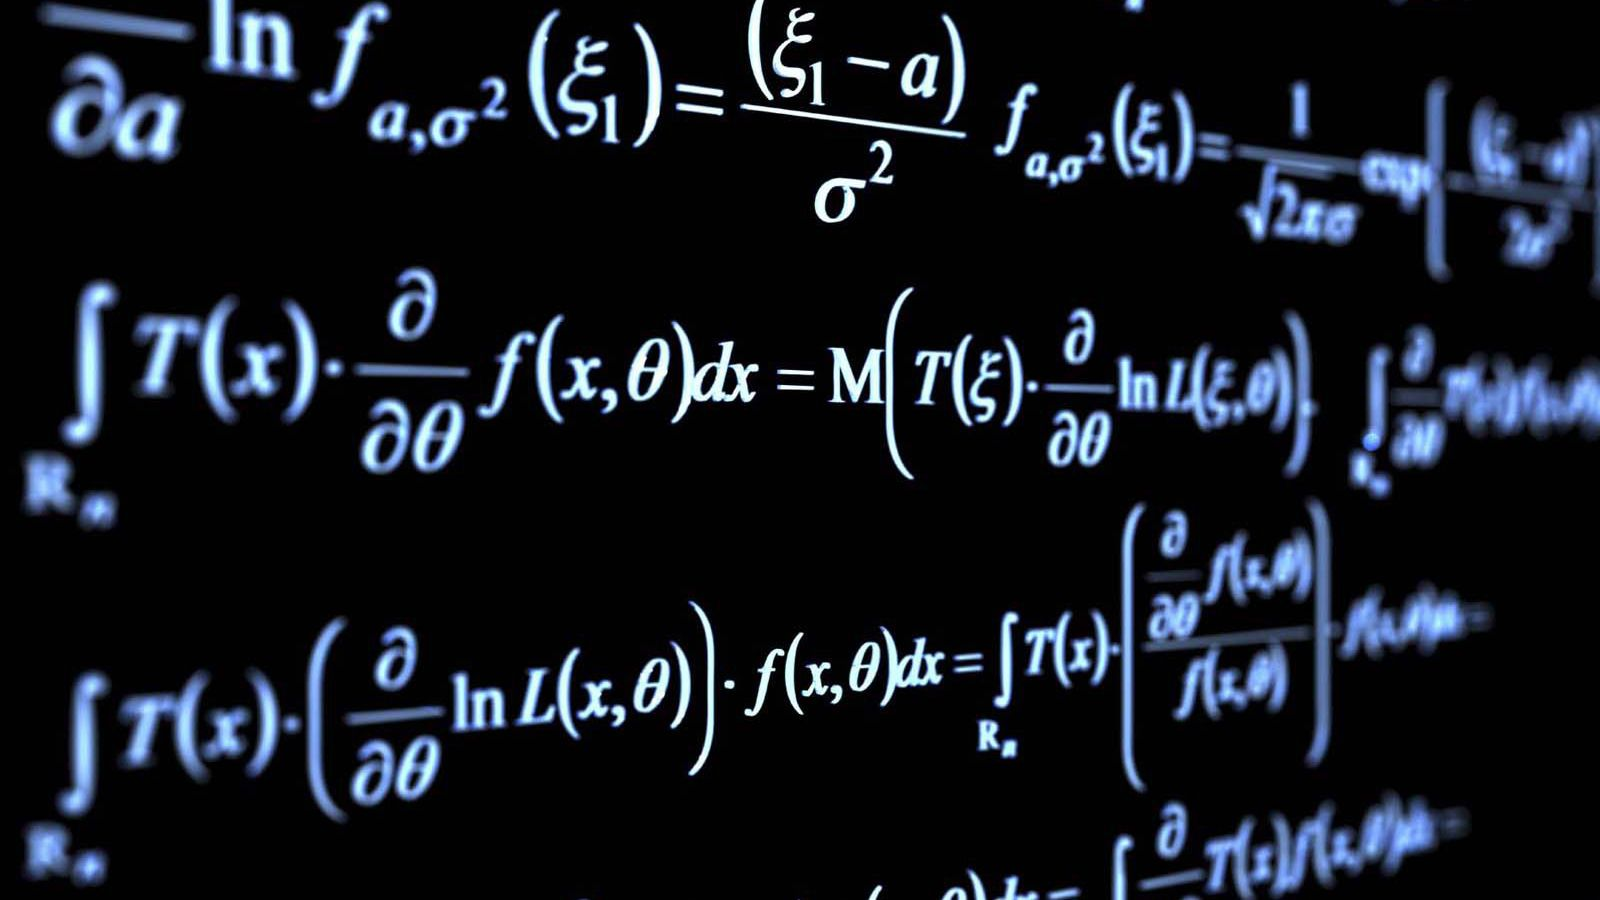
\includegraphics[height=13.88cm, width=17cm, keepaspectratio]{Pics/maths.jpg}
\end{center}

\chapter{Essential Mathematical Techniques}%
\phantomsection                      % <-- creates a hyperlink anchor
\label{sec:maths}

\begin{itemize}
    \item \textbf{Modular Arithmetic:}
    \begin{itemize}
        \item $(a \pm b) \mod m = (a \mod m \pm b \mod m) \mod m$
        \item $(a \cdot b) \mod m = ((a \mod m) \cdot (b \mod m)) \mod m$
        \item Modular exponentiation: $a^b \mod m$ using binary exponentiation ($\mathcal{O}(\log b)$)
        \item Modular inverses using Fermat's little theorem ($a^{-1} \equiv a^{m-2} \pmod{m}$ for prime $m$)
    \end{itemize}
    
    \item \textbf{Prime Numbers:}
    \begin{itemize}
        \item Sieve of Eratosthenes ($\mathcal{O}(n \log \log n)$ for primes up to $n$
        \item Prime factorization via trial division ($\mathcal{O}(\sqrt{n})$)
        \item Miller-Rabin primality test (probabilistic, efficient for large numbers)
        \item Count of divisors and sum of divisors formulas from prime factors
    \end{itemize}
    
    \item \textbf{GCD \& LCM:}
    \begin{itemize}
        \item Euclidean algorithm: $\gcd(a,b) = \gcd(b, a \mod b)$
        \item $\gcd(a,b) \cdot lcm(a,b) = |a \cdot b|$
        \item Extended Euclidean algorithm for solving $ax + by = \gcd(a,b)$
    \end{itemize}
    
    \item \textbf{Combinatorics:}
    \begin{itemize}
        \item Precompute factorials and inverse factorials modulo $m$ ($\mathcal{O}(n)$)
        \item Combinations: $C(n,k) = \frac{n!}{k!(n-k)!}$; $C(n,k) = C(n-1,k-1) + C(n-1,k)$
        \item Lucas theorem for binomial coefficients modulo prime
        \item Stars and bars technique for non-negative integer solutions
    \end{itemize}
    
    \item \textbf{Number Theory:}
    \begin{itemize}
        \item Chinese Remainder Theorem (CRT) for solving system of congruences
        \item Euler's totient function: $\phi(n)$ and Euler's theorem $a^{\phi(m)} \equiv 1 \pmod{m}$ for $\gcd(a,m)=1$
        \item Wilson's theorem: $(p-1)! \equiv -1 \pmod{p}$ for prime $p$
    \end{itemize}
    
    \item \textbf{Binary Exponentiation:}
    \begin{itemize}
        \item Compute $a^n$ in $\mathcal{O}(\log n)$ time
        \item Matrix exponentiation for linear recurrences (e.g., Fibonacci in $\mathcal{O}(\log n)$)
        \item Apply to polynomials and transformations
    \end{itemize}
    
    \item \textbf{Game Theory:}
    \begin{itemize}
        \item Nim game: XOR of pile values ($\neq 0$ → winning position)
        \item Grundy numbers (mex function) for impartial games
        \item Sprague-Grundy theorem for composite games
    \end{itemize}
    
    \item \textbf{Series \& Sequences:}
    \begin{itemize}
        \item Arithmetic series: $S_n = \frac{n}{2}(2a + (n-1)d)$
        \item Geometric series: $S_n = a\frac{r^n-1}{r-1}$ ($r \neq 1$)
        \item Harmonic series: $H_n \approx \ln n + \gamma$ (Euler's constant)
        \item Faulhaber's formula for power sums $\sum k^p$
    \end{itemize}
    
    \item \textbf{Inequalities:}
    \begin{itemize}
        \item AM-GM inequality: $\frac{a_1+\cdots+a_n}{n} \geq \sqrt[n]{a_1 \cdots a_n}$
        \item Cauchy-Schwarz: $(\sum a_i b_i)^2 \leq (\sum a_i^2)(\sum b_i^2)$
        \item Chebyshev's inequality for monotonic sequences
    \end{itemize}
    
    \item \textbf{Probability \& Expectation:}
    \begin{itemize}
        \item Linearity of expectation: $E[X+Y] = E[X] + E[Y]$ even for dependent variables
        \item Geometric distribution: Expected trials until success $= \frac{1}{p}$
        \item Markov chains and absorbing states
    \end{itemize}
    
    \item \textbf{Geometry Formulas:}
    \begin{itemize}
        \item Shoelace formula for polygon area
        \item Pick's theorem: $A = I + B/2 - 1$ for lattice polygons
        \item Convex hull (Graham scan), line intersection, point-in-polygon
    \end{itemize}
    
    \item \textbf{Optimization Techniques:}
    \begin{itemize}
        \item Precomputation (sieve, factorials, prefix sums)
        \item Binary search on answer (monotonic functions)
        \item Two pointers technique for subarray problems
    \end{itemize}
    
    \item \textbf{Critical Edge Cases:}
    \begin{itemize}
        \item Integer overflow (use \texttt{long long} or modulo)
        \item Division by zero and negative modulo handling
        \item Floating point precision issues (use epsilon comparison)
        \item Boundary conditions (n=0, n=1, large inputs)
    \end{itemize}
    
    \item \textbf{Common Problem Patterns:}
    \begin{itemize}
        \item Counting problems (combinatorics + modular arithmetic)
        \item Digit DP for number property queries
        \item Diophantine equations ($ax + by = c$)
        \item Multiplicative function properties ($\phi$, $\mu$, divisor functions) 


    \end{itemize}
\end{itemize}

\section{Mathematics-Based DSA Problems Summary Table}
\begin{longtable}{|>{\raggedright\arraybackslash}p{3.2cm}|>{\columncolor{c2}\centering\arraybackslash}p{2.5cm}|>{\columncolor{c3}\raggedright\arraybackslash}p{4.3cm}|>{\columncolor{c4}\raggedright\arraybackslash}p{3.5cm}|>{\columncolor{c5}\color{white}\raggedright\arraybackslash}p{3.5cm}|}
\hline
\rowcolor{rclr}
\textbf{Problem Name} & \textbf{Time Complexity} & \textbf{Idea to Solve} & \textbf{Optimization Tip} & \textbf{Edge Cases} \\
\hline
\endfirsthead

\hline
\textbf{Problem Name} & \textbf{Time Complexity} & \textbf{Idea to Solve} & \textbf{Optimization Tip} & \textbf{Edge Cases} \\
\hline
\endhead

Count Digits & $\mathcal{O}(\log_{10} N)$ & Divide number by 10 repeatedly. & Use $\lfloor \log_{10}N \rfloor + 1$ formula. & $N = 0$ (special case) \\
\hline
Palindrome Number & $\mathcal{O}(\log_{10} N)$ & Reverse number and compare with original. & Reverse half only to save time. & Negative numbers, numbers ending in 0 \\
\hline
Factorial of a Number & $\mathcal{O}(N)$ & Multiply from 1 to $N$ iteratively. & Use memoization if computed repeatedly. & Overflow for large $N$ \\
\hline
Trailing Zeros in Factorial & $\mathcal{O}(\log_5 N)$ & Count number of 5s in prime factorization. & Precompute for multiple queries. & $N < 5$ \\
\hline
GCD / HCF & $\mathcal{O}(\log \min(a,b))$ & Use Euclidean algorithm TC drivat. by fibonacci steps (increase by 1). & Use iterative form to avoid recursion stack. & $a=0$, $b=0$ \\
\hline
LCM of Two Numbers & $\mathcal{O}(\log \min(a,b))$ & $\text{LCM} = \frac{a \cdot b}{\text{GCD}}$ & Avoid overflow using $(a/\text{GCD}) \cdot b$ & One of them is 0 \\
\hline
Check for Prime & $\mathcal{O}(\sqrt{N})$ & Trial division up to $\sqrt{N}$ & Check only up to odd numbers and skip even & $N < 2$, very large $N$ \\
\hline
Prime Factors & $\mathcal{O}(\sqrt{N})$ & Divide repeatedly by prime numbers. & Use Sieve for multiple queries. & $N=1$, $N$ is prime \\
\hline
All Divisors of a Number & $\mathcal{O}(\sqrt{N})$ & Check all $i$ where $i \mid N$ and also $N/i$. & Store in a set to avoid duplicates. & Perfect square, $N=1$ \\
\hline
Sieve of Eratosthenes & $\mathcal{O}(N \log \log N)$ & Use boolean array to mark non-primes. & Skip even numbers to reduce space/time. & $N < 2$ \\
\hline
Computing Power ($a^b$) & $\mathcal{O}(\log b)$ & Use exponentiation by squaring. & Apply modulus if result is large. & $b=0$, $a=0$ \\
\hline
Modular Arithmetic & $\mathcal{O}(1)$ & Apply modulo rules: $(a \pm b)\%m$, etc. & Handle underflow: use $((a\%m)+m)\%m$ & Negative numbers, division mod \\
\hline
Iterative Power & $\mathcal{O}(\log b)$ & Binary exponentiation. & Use bitwise operations for speed. & $a=0$, $b=0$ \\
\hline

\end{longtable}
\clearpage
\newgeometry{margin=1in}
% \documentclass[a4paper,10pt]{article}
% \usepackage[utf8]{inputenc}
% \usepackage{geometry}
% \usepackage[table]{xcolor}
% \usepackage{colortbl}
% \usepackage{color,soul}
% \geometry{margin=0.8in}
% \usepackage{xcolor}
% \usepackage{tikz}
% \usepackage{minted}
% \usepackage{standalone}
% \definecolor{bgcolor}{rgb}{0.8, 0.9, 0.5} % 
% \definecolor{bgcolor1}{rgb}{0.95, 0.95, 0.95} % Light Gray
% \definecolor{bgcolor2}{rgb}{0.85, 0.92, 1.0}  % Soft Blue
% \definecolor{bgcolor3}{rgb}{0.9, 0.85, 1.0}   % Light Purple
% \definecolor{bgcolor4}{rgb}{0.95, 0.88, 0.76} % Warm Beige
% \definecolor{bgcolor5}{rgb}{0.8, 0.95, 0.8}   % Gentle Green
% \definecolor{bgcolor6}{rgb}{1.0, 0.87, 0.87}  % Pastel Red
% \definecolor{bgcolor7}{rgb}{0.86, 0.93, 0.83} % Mint Green
% \definecolor{bgcolor8}{rgb}{0.98, 0.85, 0.94} % Soft Pink
% \definecolor{bgcolor9}{rgb}{0.87, 0.94, 0.98} % Sky Blue
% \definecolor{bgcolor10}{rgb}{0.96, 0.96, 0.82} % Pale Yellow
% 
% % Define a custom background colo
% \begin{document}
\section*{Mathematics Problem Solutions}

\noindent\textbf{Problem: Palindrome Number}
\begin{minted}[
    bgcolor=bgcolor7,
    frame=lines,
    framesep=5mm,
    rulecolor=\color{black},
    linenos,
    numbersep=5pt,
    fontsize=\normalsize
]{python}
def is_palindrome_number(n: int) -> bool:
    """
    Check if n reads the same forward and backward.
    Time Complexity: O(log10 N)
    """
    if n < 0 or (n % 10 == 0 and n != 0):
        return False
    rev_half = 0
    while n > rev_half:
        rev_half = rev_half * 10 + n % 10
        n //= 10
    return n == rev_half or n == rev_half // 10
\end{minted}
\noindent\textbf{Problem: Factorial of a Number}
\begin{minted}[
    bgcolor=bgcolor2,
    frame=lines,
    framesep=5mm,
    rulecolor=\color{black},
    linenos,
    numbersep=5pt,
    fontsize=\normalsize
]{python}
def factorial(n: int, memo: dict[int,int]=None) -> int:
    """
    Compute n! iteratively or via memoization.
    Time Complexity: O(N)
    """
    if memo is None:
        memo = {}
    if n < 2:
        return 1
    if n in memo:
        return memo[n]
    result = 1
    for i in range(2, n + 1):
        result *= i
    memo[n] = result
    return result
\end{minted}
\noindent\textbf{Problem: Trailing Zeros in Factorial}
\begin{minted}[
    bgcolor=bgcolor9,
    frame=lines,
    framesep=5mm,
    rulecolor=\color{black},
    linenos,
    numbersep=5pt,
    fontsize=\normalsize
]{python}
def trailing_zeros(n: int) -> int:
    """
    Count how many trailing zeros n! has by counting factors of 5.
    Time Complexity: O(log_5 N)"""
    count = 0
    while n >= 5:
        n //= 5
        count += n
    return count
\end{minted}
\noindent\textbf{Problem: GCD / HCF}
\begin{minted}[
    bgcolor=bgcolor5,
    frame=lines,
    framesep=5mm,
    rulecolor=\color{black},
    linenos,
    numbersep=5pt,
    fontsize=\normalsize
]{python}
def gcd(a: int, b: int) -> int:
    """
    Compute the greatest common divisor using Euclid’s algorithm.
    Time Complexity: O(log min(a, b))
    """
    a, b = abs(a), abs(b)
    while b:
        a, b = b, a % b
    return a
\end{minted}
\noindent\textbf{Problem: Check for Prime}
\begin{minted}[
  bgcolor=bgcolor6,
  frame=lines,
  framesep=5mm,
  rulecolor=\color{black},
  linenos,
  numbersep=5pt,
  fontsize=\normalsize
]{python}
def is_prime(n: int) -> bool:
    """
    Check if n is prime using 6k±1 optimization.
    Time Complexity: O(root(N)) 
    """
    if n < 2:
        return False
    if n in (2, 3):
        return True
    if n % 2 == 0 or n % 3 == 0:
        return False
    i = 5
    while i * i <= n:
        if n % i == 0 or n % (i + 2) == 0:
            return False
        i += 6

    return True
\end{minted}

\noindent\textbf{Problem: Prime Factors}
\begin{minted}[
    bgcolor=bgcolor1,
    frame=lines,
    framesep=5mm,
    rulecolor=\color{black},
    linenos,
    numbersep=5pt,
    fontsize=\normalsize
]{python}
def prime_factors(n: int) -> list[int]:
    """
    Return the list of prime factors of n using 6k±1 optimization.
    Time Complexity: O(root(N))
    """
    factors = []
    # remove all 2s
    while n % 2 == 0:
        factors.append(2)
        n //= 2
    # remove all 3s
    while n % 3 == 0:
        factors.append(3)
        n //= 3
    # now test 6k±1
    i = 5
    while i * i <= n:
        # factor = i
        while n % i == 0:
            factors.append(i)
            n //= i
        # factor = i + 2
        while n % (i + 2) == 0:
            factors.append(i + 2)
            n //= (i + 2)
        i += 6
    # if n is still >1, it’s prime
    if n > 1:
        factors.append(n)
    return factors
\end{minted}
\noindent\textbf{Problem: All Divisors of a Number}
\begin{minted}[
    bgcolor=bgcolor10,
    frame=lines,
    framesep=5mm,
    rulecolor=\color{black},
    linenos,
    numbersep=5pt,
    fontsize=\normalsize
]{python}
def all_divisors(n: int) -> list[int]:
    """
    Return all divisors of n in ascending order.
    Time Complexity: O(root(N))"""
    small, large = [], []
    i = 1
    while i * i <= n:
        if n % i == 0:
            small.append(i)
            if i != n // i:
                large.append(n // i)
        i += 1
    return small + large[::-1]
\end{minted}
\noindent\textbf{Problem: Sieve of Eratosthenes}
\begin{minted}[
    bgcolor=bgcolor3,
    frame=lines,
    framesep=5mm,
    rulecolor=\color{black},
    linenos,
    numbersep=5pt,
    fontsize=\normalsize
]{python}
def sieve(n: int) -> list[bool]:
    """
    Generate a boolean list is_prime[0..n] using the sieve.
    Time Complexity: O(n log log n)
    """
    if n < 2:
        return [False] * (n + 1)
    is_prime = [True] * (n + 1)
    is_prime[0:2] = [False, False]
    for p in range(3, int(n**0.5) + 1, 2):
        if is_prime[p]:
            for multiple in range(p*p, n + 1, 2*p):
                is_prime[multiple] = False
    return is_prime
\end{minted}
\noindent\textbf{Problem: Computing Power (Recursive)}
\begin{minted}[
    bgcolor=bgcolor6,
    frame=lines,
    framesep=5mm,
    rulecolor=\color{black},
    linenos,
    numbersep=5pt,
    fontsize=\normalsize
]{python}
def power_recursive(a: float, b: int) -> float:
    """
    Compute a**b via exponentiation by squaring (recursive).
    Time Complexity: O(log b)    """
    if b == 0:
        return 1
    half = power_recursive(a, b // 2)
    return half * half if b % 2 == 0 else half * half * a
\end{minted}
\noindent\textbf{Problem: Iterative Power}
\begin{minted}[
    bgcolor=bgcolor2,
    frame=lines,
    framesep=5mm,
    rulecolor=\color{black},
    linenos,
    numbersep=5pt,
    fontsize=\normalsize
]{python}
def power_iterative(a: float, b: int) -> float:
    """
    Compute a**b via binary exponentiation (iterative).
    Time Complexity: O(log b)    """
    result = 1.0
    base = a
    exp = b
    while exp > 0:
        if exp & 1:
            result *= base
        base *= base
        exp >>= 1
    return result
\end{minted}
\noindent\textbf{Problem: Modular Arithmetic}
\begin{minted}[
    bgcolor=bgcolor4,
    frame=lines,
    framesep=5mm,
    rulecolor=\color{black},
    linenos,
    numbersep=5pt,
    fontsize=\normalsize
]{python}
def mod_pow(a: int, b: int, m: int) -> int:
    """
    Compute (a**b) mod m using fast exponentiation.
    Time Complexity: O(log b)    """
    result = 1
    base = a % m
    exp = b
    while exp > 0:
        if exp & 1:
            result = (result * base) % m
        base = (base * base) % m
        exp >>= 1
    return result
\end{minted}
% \end{document}

\newgeometry{margin=0.2in}
\vspace*{47mm}

\begin{center}

{\fontsize{55}{20}\selectfont \textcolor{headingcolor}{\bfseries BIT-MANIPULATION}}
\end{center}

\vspace{50mm}

\begin{center}

\includegraphics[height=13.88cm, width=17cm, keepaspectratio]{Pics/bits.png}
\end{center}
\chapter{Essential Bit Manipulation Techniques  }
\phantomsection                      % <-- creates a hyperlink anchor
\label{sec:bits}
\begin{itemize}
    \item \textbf{Power of Two Check:}
    \begin{itemize}
        \item ${n \& (n-1) == 0 \&\& n != 0}$
        \item Clears least significant set bit (e.g., $8 \rightarrow 1000$, $7 \rightarrow 0111$)
    \end{itemize}
    
    \item \textbf{XOR Properties:}
    \begin{itemize}
        \item $a \oplus a = 0$, $a \oplus 0 = a$
        \item $a \oplus b = b \oplus a$ (commutative)
        \item $(a \oplus b) \oplus c = a \oplus (b \oplus c)$ (associative)
        \item Useful for finding missing numbers/canceling pairs
    \end{itemize}
    
    \item \textbf{Mask Operations:}
    \begin{itemize}
        \item Set $k$-th bit: \texttt{n | (1 << k)}
        \item Clear $k$-th bit: \texttt{n \& \textasciitilde(1 << k)}
        \item Toggle bit: \texttt{n \^{} (1 << k)}
        \item Check bit: \texttt{(n >> k) \& 1}
    \end{itemize}
    
    \item \textbf{Brian Kernighan's Algorithm:}
    \begin{itemize}
        \item Count set bits with \texttt{while (n) { count++; n \&= n-1; }}
        \item Complexity: $\mathcal{O}(\text{\# set bits})$ instead of $\mathcal{O}(n)$
    \end{itemize}
    
    \item \textbf{Rightmost Set Bit:}
    \begin{itemize}
        \item Isolate: \texttt{n \& -n} (using two's complement)
        \item Clear: \texttt{n \&= n-1}
    \end{itemize}
    
    \item \textbf{Swapping Without Temp:}
    \begin{itemize}
        \item \texttt{a \^{}= b; b \^{}= a; a \^{}= b;}
    \end{itemize}
    
    \item \textbf{Signed Shift vs Unsigned Shift:}
    \begin{itemize}
        \item Logical right shift (\texttt{>>>}): Fill with 0s
        \item Arithmetic right shift (\texttt{>>}): Preserve sign bit
    \end{itemize}
    
    \item \textbf{Subset Generation:}
    \begin{itemize}
        \item Power sets via bitmask: \texttt{for (int i=0; i < (1<<n); i++)}
        \item Extract elements: \texttt{if (i \& (1 << j))}
    \end{itemize}
    
    \item \textbf{Advanced Patterns:}
    \begin{itemize}
        \item XOR from 1 to $n$: Pattern repeats every 4 (mod 4)
        \item Swap adjacent bits: \texttt{((n \& 0xAAAAAAAA) >> 1) | ((n \& 0x55555555) << 1)}
        
        \item Reverse bits: Divide \& conquer with masks
    \end{itemize}
    
    \item \textbf{Optimization Tricks:}
    \begin{itemize}
        \item Precompute bit counts for small chunks (lookup table)
        \item Use integer as boolean array (bit sets)
        
        \item Parallel bit operations (e.g., count set bits with magic numbers)
    \end{itemize}
    
    \item \textbf{Critical Edge Cases:}
    \begin{itemize}
        \item Negative numbers (two's complement representation)
        \item Integer overflow in shifts (e.g., \texttt{1 << 31} in 32-bit)
        \item Shifting by $\geq$ bit width (undefined behavior)
        \item Zero handling (especially in power-of-two checks)
    \end{itemize}
    
    \item \textbf{Common Problem Patterns:}
    \begin{itemize}
        \item Single Number (XOR all elements)
        \item Bitwise AND of number range (find common MSB prefix)
        \item Minimum Flips (XOR + count bits)
        \item Bitwise OR/AND subarrays (property observation)
    \end{itemize}
\end{itemize}
\section{Bit-Manipulation-Based DSA Problems Summary Table}
\begin{longtable}{|>{\raggedright\arraybackslash}p{3.2cm}|>{\columncolor{c2}\centering\arraybackslash}p{2.5cm}|>{\columncolor{c3}\raggedright\arraybackslash}p{4.3cm}|>{\columncolor{c4}\raggedright\arraybackslash}p{3.5cm}|>{\columncolor{c5}\color{white}\raggedright\arraybackslash}p{3.5cm}|}
\hline
\rowcolor{rclr}
\textbf{Problem Name} & \textbf{Time Complexity} & \textbf{Idea to Solve} & \textbf{Optimization Tip} & \textbf{Edge Cases} \\
\hline
\endfirsthead

\hline
\textbf{Problem Name} & \textbf{Time Complexity} & \textbf{Idea to Solve} & \textbf{Optimization Tip} & \textbf{Edge Cases} \\
\hline
\endhead

Check if Number is Power of 2 & $\mathcal{O}(1)$ & If $n > 0$ and $(n \& (n - 1)) == 0$, then it's a power of 2. & Avoid loop-based or recursive approaches. & $n = 0$, $n < 0$ (not valid inputs) \\
\hline

XOR of All Numbers from 1 to N & $\mathcal{O}(1)$ & Use pattern based on $n \mod 4$:  
$0 \Rightarrow n$,  
$1 \Rightarrow 1$,  
$2 \Rightarrow n+1$,  
$3 \Rightarrow 0$. & Use formula for large inputs or multiple queries. & Test with $n = 0$, $n = 1$ \\
\hline

Check if Kth Bit is Set & $\mathcal{O}(1)$ & Use $(n \& (1 \ll k))$ or $(n \gg k) \& 1$ to check. & Prefer bitwise operations over string conversions. & $k$ exceeds number of bits in $n$ \\
\hline

Count Set Bits & $\mathcal{O}(\log N)$ & Use Brian Kernighan's algorithm: repeatedly turn off the rightmost set bit. & Use lookup table (precomputed bits for 0–255) in repeated use. & $n = 0$ (has 0 set bits) \\
\hline
Convert Any Base to Any Base & $O(\log N)$ & Convert source → decimal → target base by repeated division & Handle fractional part separately for floating bases & Leading zeros, invalid chars \\
\hline
Floating Point Decimal to Binary & $O(\log I + F)$ & Convert integer normally; multiply fraction by 2 repeatedly for fractional part & Limit fractional precision to 32 bits max & Infinite fractions (e.g., 0.1) \\
\hline
Longest Sequence of 1s by One Bit Flip & $O(\log N)$ & Track current streaks of 1s and possible merge with one 0 in between & Store left, right streaks and merge via window & All 1s or all 0s \\
\hline
Pairwise Swap Bits in Integer & $O(1)$ & Swap even and odd bits using masks: ((n \& 0xAAAAAAAA) >> 1) | ((n \& 0x55555555) << 1) & Use 32-bit constants for masking & Small integers (e.g., < 4-bit) \\
\hline
Two Odd Occurring Numbers & $\mathcal{O}(n)$ & XOR all elements to get XOR of the two odd numbers, then use a set bit to divide into two groups. & Use rightmost set bit to split numbers efficiently. & All other numbers must appear even number of times \\
\hline

Power Set using Bitwise & $\mathcal{O}(2^n \cdot n)$ & Each subset can be generated by using bitmasks from 0 to $2^n - 1$. & Use bitmasking instead of recursion for simplicity. & Empty set, duplicate elements \\
\hline

Maximum AND Value of Pair in Array & $\mathcal{O}(n \log n)$ & Try fixing bits from MSB to LSB, keeping candidates that can satisfy AND condition. & Use filtering based on current mask during iteration. & All elements same or small values \\
\hline
Divide Two Integers using Bit Manipulation & $O(\log n)$ & Subtract shifted divisor (left shift until <= dividend), accumulate result & Handle negatives using sign variable & Overflow (INT\_MIN / -1) \\
\hline

\end{longtable}
\clearpage

\newgeometry{margin=1in}
% \documentclass[a4paper,10pt]{article}
% \usepackage[utf8]{inputenc}
% \usepackage{geometry}
% \usepackage[table]{xcolor}
% \usepackage{colortbl}
% \usepackage{color,soul}
% \geometry{margin=0.8in}
% \usepackage{xcolor}
% \usepackage{tikz}
% \usepackage{minted}
% \definecolor{bgcolor}{rgb}{0.8, 0.9, 0.5} % 
% \definecolor{bgcolor1}{rgb}{0.95, 0.95, 0.95} % Light Gray
% \definecolor{bgcolor2}{rgb}{0.85, 0.92, 1.0}  % Soft Blue
% \definecolor{bgcolor3}{rgb}{0.9, 0.85, 1.0}   % Light Purple
% \definecolor{bgcolor4}{rgb}{0.95, 0.88, 0.76} % Warm Beige
% \definecolor{bgcolor5}{rgb}{0.8, 0.95, 0.8}   % Gentle Green
% \definecolor{bgcolor6}{rgb}{1.0, 0.87, 0.87}  % Pastel Red
% \definecolor{bgcolor7}{rgb}{0.86, 0.93, 0.83} % Mint Green
% \definecolor{bgcolor8}{rgb}{0.98, 0.85, 0.94} % Soft Pink
% \definecolor{bgcolor9}{rgb}{0.87, 0.94, 0.98} % Sky Blue
% \definecolor{bgcolor10}{rgb}{0.96, 0.96, 0.82} % Pale Yellow
% 
% % Define a custom background colo
% \begin{document}
\section*{Bit-Manipulation Problem Solutions}

    \noindent\textbf{Problem: XOR of All Numbers from 1 to N}
    \begin{minted}[
        bgcolor=bgcolor9,
        frame=lines,
        framesep=5mm,
        rulecolor=\color{black},
        linenos,
        numbersep=5pt,
        fontsize=\normalsize
    ]{python}
def xor_1_to_n(n: int) -> int:
    """
    Compute XOR of all integers from 1 up to n in O(1) time
    by exploiting the pattern of prefix XORs modulo 4.
    """
    # Using n & 3 is a fast bitwise trick for n % 4.(For 2^x can use & with 2^x -1)
    r = n & 3
    if r == 0:
        # Sequence ends in 0 ^ 1 ^ … ^ (4k−1) ^ 4k;
        # every block of 4 numbers has XOR = 0 ^ 1 ^ 2 ^ 3 = 0,
        # so only the last term (n) remains.
        return n
    if r == 1:
        # One extra element beyond a multiple of 4: … ^ (4k) ^ (4k+1)
        # gives 0 ^ (4k+1) = 4k+1, but since 4k cancels to 0 we get 1.
        return 1
    if r == 2:
        # Two extra: … ^ (4k) ^ (4k+1) ^ (4k+2)
        # = (0 ^ 1) ^ 2 = 1 ^ 2 = 3 → which equals n+1 when n=4k+2.
        return n + 1
    # r == 3
    # Three extra: … ^ (4k) ^ (4k+1) ^ (4k+2) ^ (4k+3)
    # = ((0^1)^2)^3 = 3^3 = 0
    return 0

    \end{minted}

    \noindent\textbf{Problem: Two Odd Occurring Numbers}
    \begin{minted}[
        bgcolor=bgcolor5,
        frame=lines,
        framesep=5mm,
        rulecolor=\color{black},
        linenos,
        numbersep=5pt,
        fontsize=\normalsize
    ]{python}
    from typing import Tuple, List

    def two_odd_occurring(arr: List[int]) -> Tuple[int,int]:
        """
        In an array where exactly two numbers appear odd times and others even,
        return the two odd-occurring numbers.
        Time Complexity: O(n)
        """
        xor_all = 0
        for x in arr:
            xor_all ^= x
        # isolate rightmost set bit
        mask = xor_all & -xor_all
        a = b = 0
        for x in arr:
            if x & mask:
                a ^= x
            else:
                b ^= x
        return a, b
    \end{minted}

    \noindent\textbf{Problem: Power Set using Bitwise}
    \begin{minted}[
        bgcolor=bgcolor10,
        frame=lines,
        framesep=5mm,
        rulecolor=\color{black},
        linenos,
        numbersep=5pt,
        fontsize=\normalsize
    ]{python}
    from typing import List

    def power_set(arr: List[int]) -> List[List[int]]:
        """
        Generate all subsets of arr using bit-masking.
        Time Complexity: O(2^n · n)
        """
        n = len(arr)
        result = []
        for mask in range(1 << n):
            subset = [arr[i] for i in range(n) if mask & (1 << i)]
            result.append(subset)
        return result
    \end{minted}

    \noindent\textbf{Problem: Maximum AND Value of Pair in Array}
    \begin{minted}[
        bgcolor=bgcolor3,
        frame=lines,
        framesep=5mm,
        rulecolor=\color{black},
        linenos,
        numbersep=5pt,
        fontsize=\normalsize
    ]{python}
    from typing import List

    def max_pair_and(arr: List[int]) -> int:
        """
        Find maximum (x & y) over all pairs in arr by filtering bits top-down.
        Time Complexity: O(n · log MAX)
        """
        res = 0
        for bit in range(arr[0].bit_length(), -1, -1):
            candidate = res | (1 << bit)
            count = sum(1 for x in arr if (x & candidate) == candidate)
            if count >= 2:
                res = candidate
        return res
    \end{minted}

    \noindent\textbf{Problem: Divide Two Integers using Bit Manipulation}
    \begin{minted}[
        bgcolor=bgcolor8,
        frame=lines,
        framesep=5mm,
        rulecolor=\color{black},
        linenos,
        numbersep=5pt,
        fontsize=\normalsize
    ]{python}
    def divide(dividend: int, divisor: int) -> int:
    """
    Divide dividend by divisor without using / or * operators.
    Time Complexity: O(log |dividend|)
    """
    if divisor == 0:
        raise ZeroDivisionError("division by zero")
    sign = -1 if (dividend < 0) ^ (divisor < 0) else 1
    a, b = abs(dividend), abs(divisor)
    result = 0

    # “Bring down” bits one by one, from highest to lowest
    #    a.bit_length()–1 is the index of dividend’s top bit.
    for shift in range(a.bit_length() - 1, -1, -1):
        #  Try to subtract (divisor << shift) from current remainder a
        if (b << shift) <= a:
            a -= b << shift             # subtract that chunk
            result |= 1 << shift        # like for 10,3 check with 4 then 2 then 1
    return sign * result

    \end{minted}
% \end{document}

\newgeometry{margin=0.2in}
\vspace*{47mm}

\begin{center}

{\fontsize{55}{20}\selectfont \textcolor{headingcolor}{\bfseries ARRAYS}}
\end{center}

\vspace{50mm}

\begin{center}
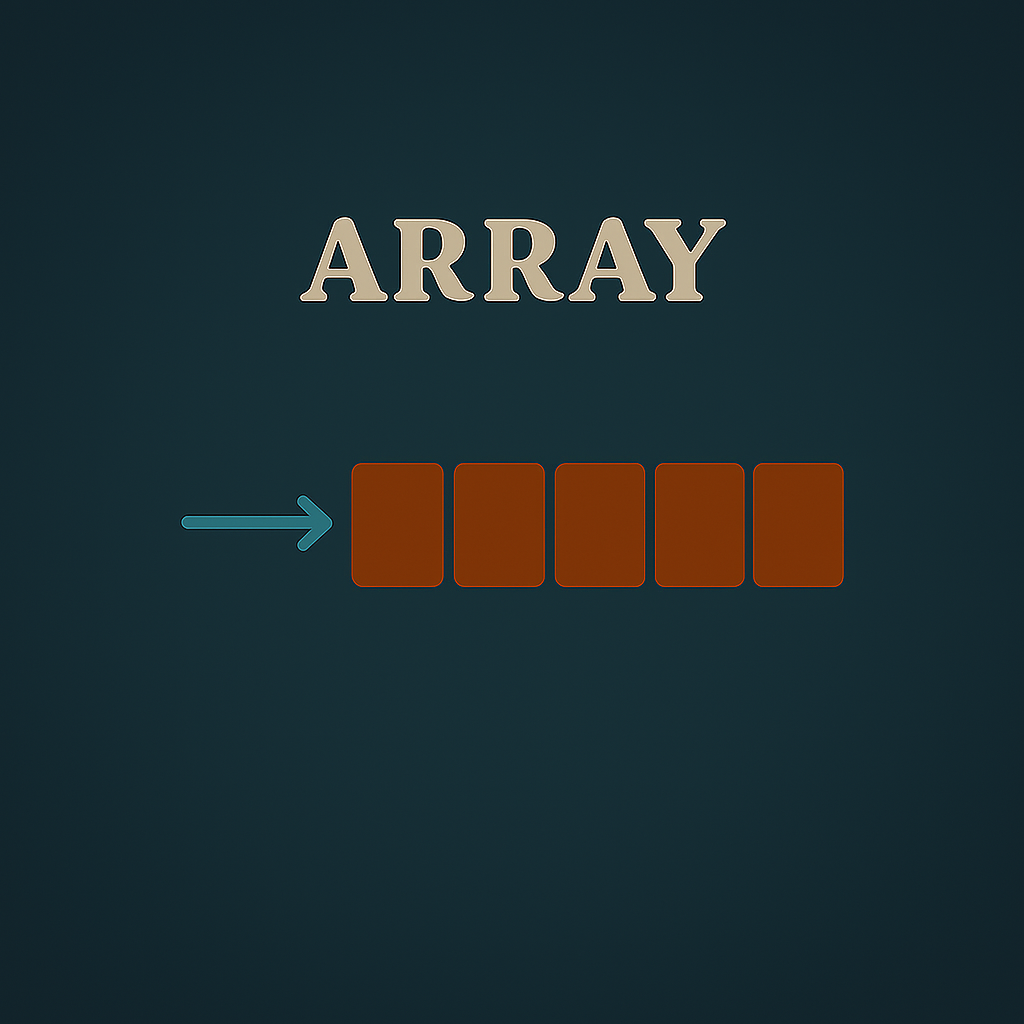
\includegraphics[height=13.88cm, width=17cm, keepaspectratio]{Pics/array.png}
\end{center}

\chapter{Essential Array Techniques  }
\phantomsection                      % <-- creates a hyperlink anchor
\label{sec:arrays}
Most important step in arrays question is to think about all the different possible test cases that you can generate. Then observe them to see what pattern they are following.
\begin{itemize}[leftmargin=*]
    \item \textbf{Two Pointer Technique:}
    \begin{itemize}
        \item Same Direction Pointers: Use when you need to maintain a window or process elements sequentially
        \item Opposite Direction Pointers: Ideal for sorted arrays, palindrome checks, or pair sum problems
        \item Fast-Slow Pointers: Detect cycles, find middle elements, or remove duplicates
        \item Key Pattern: Always consider if you can reduce $O(n^2)$ to $O(n)$ using two pointers
    \end{itemize}
    
    \item \textbf{Sliding Window:}
    \begin{itemize}
        \item Fixed Size Window: When subarray/substring length is constant
        \item Variable Size Window: When you need to find optimal window based on conditions
        \item Shrinking Strategy: Expand right pointer first, then shrink left when condition violated
        \item Template: Maintain window state using hash maps or frequency arrays
        \item Positive,Negative,Zero : Containing arrays when to use $<=$ target
    \end{itemize}
    
    \item \textbf{Prefix Sum Techniques:}
    \begin{itemize}
        \item 1D Prefix Sum: $prefix[i] = prefix[i-1] + arr[i]$ for range sum queries
        \item 2D Prefix Sum: For matrix range sum queries in $O(1)$ time
        \item Prefix XOR: Useful for subarray XOR problems
        \item Hash Map + Prefix: Store prefix sums to find subarrays with target sum
    \end{itemize}
\end{itemize}

\begin{itemize}[leftmargin=*]
    \item \textbf{Monotonic Stack/Deque:}
    \begin{itemize}
        \item Next Greater Element: Maintain decreasing stack
        \item Largest Rectangle: Classic histogram problem using monotonic stack
        \item Sliding Window Maximum: Use monotonic deque for $O(n)$ solution
        \item Pattern Recognition: When you need to find next/previous greater/smaller elements
    \end{itemize}
    
    \item \textbf{Binary Search on Arrays:}
    \begin{itemize}
        \item Search Space: Identify the range where answer can exist
        \item Monotonic Property: Ensure the search space has a monotonic property
        \item Template: Use $left + (right - left) / 2$ to avoid overflow
        \item Edge Cases: Handle empty arrays, single elements, and boundary conditions
    \end{itemize}
    
    \item \textbf{Divide and Conquer:}
    \begin{itemize}
        \item Merge Sort Pattern: For inversion counting, smaller elements problems
        \item Quick Select: Finding kth element in $O(n)$ average time
        \item Maximum Subarray: Kadane's algorithm or divide-and-conquer approach
        \item Recurrence Relations: Master theorem for time complexity analysis
    \end{itemize}
\end{itemize}

\begin{itemize}[leftmargin=*]
    \item \textbf{Mathematical Insights:}
    \begin{itemize}
        \item Pigeonhole Principle: If $n+1$ elements in range $[1,n]$, at least one duplicate exists
        \item XOR Properties: $a \oplus a = 0$, $a \oplus 0 = a$, useful for finding unique elements
        \item Modular Arithmetic: Handle large numbers and cyclic patterns
        \item Dutch National Flag: Partition array into three parts efficiently
    \end{itemize}
    
    \item \textbf{Index Manipulation:}
    \begin{itemize}
        \item Negative Marking: Use array elements as indices, mark visited by negation
        \item Cyclic Sort: When array contains numbers in range $[1,n]$ or $[0,n-1]$
        \item Index as Hash: Use array positions as hash keys when range is limited
        \item In-place Algorithms: Modify array without extra space using clever indexing
    \end{itemize}
\end{itemize}

\begin{itemize}[leftmargin=*]
    \item \textbf{Subarray Problems:}
    \begin{itemize}
        \item Contiguous Elements: Use sliding window or two pointers
        \item Sum-based Conditions: Prefix sum + hash map approach
        \item Maximum/Minimum Subarray: Kadane's algorithm variants
        \item K-constraints: Often solvable with sliding window technique
    \end{itemize}
    
    \item \textbf{Frequency-based Problems:}
    \begin{itemize}
        \item Character/Number Frequency: Use hash maps or frequency arrays
        \item Anagram Detection: Sort strings or compare frequency maps
        \item Top K Elements: Use heap or quickselect algorithm
        \item Majority Element: Boyer-Moore voting algorithm for $O(1)$ space
    \end{itemize}
    
    \item \textbf{Sorting-based Solutions:}
    \begin{itemize}
        \item When to Sort: If relative order doesn't matter in final answer
        \item Custom Comparators: For complex sorting requirements
        \item Merge Intervals: Sort by start time, then merge overlapping
        \item Meeting Rooms: Sort intervals and check for conflicts
    \end{itemize}
\end{itemize}
\begin{itemize}[leftmargin=*]
    \item \textbf{Common Reductions:}
    \begin{itemize}
        \item $O(n^2) \rightarrow O(n)$: Use hash maps, two pointers, or sliding window
        \item $O(n^2) \rightarrow O(n \log n)$: Sort first, then use binary search or two pointers
        \item $O(n^3) \rightarrow O(n^2)$: Fix one variable, optimize the rest
        \item $O(n \log n) \rightarrow O(n)$: Use counting sort for limited range integers
    \end{itemize}
    
    \item \textbf{Space-Time Tradeoffs:}
    \begin{itemize}
        \item Memoization: Trade space for time in recursive solutions
        \item Hash Tables: $O(1)$ lookup at cost of $O(n)$ space
        \item In-place Modifications: Save space by modifying input array
        \item Bit Manipulation: Use bits to store multiple boolean flags (\textbf{All Unique Characters in string,Palindrome Permutation})
    \end{itemize}
\end{itemize}

\begin{itemize}[leftmargin=*]
    \item \textbf{Edge Cases to Consider:}
    \begin{itemize}
        \item Empty Array: Handle $n = 0$ case explicitly
        \item Single Element: Many algorithms need special handling for $n = 1$
        \item All Same Elements: Test with arrays containing identical elements
        \item Sorted/Reverse Sorted: Test with already sorted input
        \item Integer Overflow: Use long long for sum calculations
    \end{itemize}

    \item \textbf{Debugging Strategies:}
    \begin{itemize}
        \item Small Test Cases: Start with arrays of size 1-3
        \item Boundary Values: Test with minimum and maximum constraints
        \item Print Intermediate States: Debug by printing array states
        \item Invariant Checking: Verify loop invariants at each iteration
    \end{itemize}
\end{itemize}
\begin{itemize}[leftmargin=*]
    \item \textbf{Quick Implementation:}
    \begin{itemize}
        \item Template Preparation: Have pre-written templates for common patterns
        \item STL Mastery: Know \texttt{sort()}, \texttt{binary\_search()}, \texttt{lower\_bound()}, etc.
        \item Fast I/O: Use \texttt{ios\_base::sync\_with\_stdio(false)} for faster input
        \item Macro Usage: Define macros for frequently used code snippets
    \end{itemize}

    \item \textbf{Problem Analysis:}
    \begin{itemize}
        \item Constraint Analysis: Use constraints to determine expected time complexity
        \item Pattern Matching: Quickly identify if problem fits known patterns
        \item Simplified Version: Solve easier version first, then generalize
        \item Multiple Approaches: Think of brute force, then optimize step by step
    \end{itemize}
\end{itemize}

\section{Array-Based DSA Problems Summary Table}
\begin{longtable}{|>{\raggedright\arraybackslash}p{3.2cm}|>{\columncolor{c2}\centering\arraybackslash}p{2.5cm}|>{\columncolor{c3}\raggedright\arraybackslash}p{4.3cm}|>{\columncolor{c4}\raggedright\arraybackslash}p{3.5cm}|>{\columncolor{c5}\color{white}\raggedright\arraybackslash}p{3.5cm}|}
\hline
\rowcolor{rclr}
\textbf{Problem Name} & \textbf{Time Complexity} & \textbf{Idea to Solve} & \textbf{Optimization Tip} & \textbf{Edge Cases} \\
\hline
\endfirsthead

\hline
\rowcolor{rclr}
\textbf{Problem Name} & \textbf{Time Complexity} & \textbf{Idea to Solve} & \textbf{Optimization Tip} & \textbf{Edge Cases} \\
\hline
\endhead

Equilibrium Index of Array & $\mathcal{O}(n)$ & Calculate total sum, then iterate maintaining left sum and subtract current from total to get right sum. & Single-pass method using precomputed total sum. & All negative numbers, index at ends \\
\hline

Largest Sum Subarray (Kadane’s) & $\mathcal{O}(n)$ & Kadane’s Algorithm – track current and max sums. & Reset current sum when it drops below 0. & All negatives (return max element) \\
\hline

Merge Two Sorted Arrays & $\mathcal{O}(n + m)$ & Use two-pointer technique for merging. & Avoid extra space if merging into one array with space. & One array empty \\
\hline

Move Zeros to End & $\mathcal{O}(n)$ & Use two-pointer technique, swap non-zero elements forward. & Minimize swaps by checking index before swap. & All zeros or no zeros \\
\hline

Left Rotate Array by D Places & $\mathcal{O}(n)$ & Use reversal algorithm (reverse parts and full array). & Avoid multiple shifts with modulo $D \% n$. & $D > n$, $D = 0$ \\
\hline

Leaders in an Array & $\mathcal{O}(n)$ & Traverse from right, keep track of max seen so far. & No need to check all elements left of current. & All decreasing or increasing \\
\hline

Maximum Difference with Order & $\mathcal{O}(n)$ & Track minimum element seen so far, compute difference. & Only one pass needed using min till index. & No profit (return 0 or -1) \\
\hline

Frequencies in Sorted Array & $\mathcal{O}(n)$ & Traverse array and count frequency changes at each value. & Use binary search to find boundaries if needed. & Single element repeated \\
\hline

Stock Buy and Sell & $\mathcal{O}(n)$ & Buy at local minima, sell at next peak. Multiple transactions allowed. & Track ascending subarrays for profit. & No transaction possible \\
\hline

Maximum Circular Subarray Sum & $\mathcal{O}(n)$ & Use Kadane’s for normal max, and total sum - min subarray sum. & Handle all negative case separately. & All elements negative \\
\hline

Majority Element (Boyer-Moore) & $\mathcal{O}(n)$ & Boyer-Moore Voting Algorithm for candidate + verification. & Avoid hashmaps for optimal space. & No element appears $>$ n/2 \\
\hline

Trapping Rain Water & $\mathcal{O}(n)$ & Use two-pointer approach or precompute left/right max arrays. & Two-pointer method is space-efficient. & All increasing/decreasing \\
\hline

Minimum Consecutive Flips & $\mathcal{O}(n)$ & Count transitions and flip the smaller group. & Start from index 1 and track change points. & All same elements \\
\hline

Sliding Window Technique & $\mathcal{O}(n)$ & Maintain window sum/condition while expanding and shrinking bounds. & Reuse previous computations to update window. & k $>$ n, empty array \\
\hline
Consecutive Ones III & $O(n)$ & Sliding window with at most $k$ zeros allowed; shrink if count > k & Maintain left pointer for window & k = 0 or all 1s \\
\hline
Longest Substring with At Most K Distinct (Fruit in Basket) & $O(n)$ & Sliding window + hashmap of frequencies, shrink when map size > k & Use OrderedDict or default dict & k > distinct chars, k = 0 \\
\hline
Longest Substring Without Repeating Characters & $O(n)$ & Sliding window + set or map to track last seen index & Update left pointer when repeat found & All unique or all same \\
\hline
Binary Subarray With Sum = K & $O(n)$ & Prefix sum + hashmap count of sums: $count += freq[curr - k]$ & Use cumulative sum & Many zeros or k = 0 \\
\hline
Count All Substrings With Exactly K Distinct Chars & $O(n)$ & AtMost(K) - AtMost(K-1) using sliding window count logic & Reuse AtMost function for both & K = 0 or more than total distinct \\
\hline
Print All Substrings With Exactly K Distinct Chars & $O(n^2)$ & Iterate i from 0 to n-1, use freq map to expand j and print when distinct = k & Early break if distinct > k & Duplicates or repeated characters \\
\hline

Prefix Sum Technique & $\mathcal{O}(n)$ preprocess, $\mathcal{O}(1)$ query & Build prefix sum array to compute range sums in constant time. & Avoid recomputation of sums. & First index access, empty ranges \\
\hline

Maximum Appearing Element in Ranges & $\mathcal{O}(N + max(R))$ & Use difference array to mark increments/decrements, prefix sum to find max value. & Avoid brute force by using diff array instead of actual marking. & Multiple same max values (pick smallest index) \\
\hline

Subarray with Given Sum Count/Find. Also can find length of longest such & $\mathcal{O}(n)$ & Use sliding window for positive integers: expand until target $>=$ sum, then shrink. & Only works for positive integers for negatives go for hashing. & No valid subarray, single element solution \\
\hline
Next Permutation & $O(n)$ & Find longest non-increasing suffix, swap pivot with next larger, reverse suffix & Use STL next\_permutation if allowed & Last permutation → return first \\
\hline
Maximum Product Subarray & $O(n)$ & Two variables tracking prefix and suffix product max of them at any instance & Track current max and min due to negative flips: $max = \max(arr[i], arr[i] \cdot max, arr[i] \cdot min)$  Reset on zero & Negative numbers, multiple zeros \\
\hline
Find Rotation Count (Sorted \& Rotated Array) & $O(\log n)$ & Binary search for minimum element index & Compare with mid and neighbors & No rotation → return 0 \\
\hline
Minimum Window Substring & $O(|s|+|t|)$ & Sliding-window with two frequency maps (need/window), expand right until all required chars are met then contract left to minimize & Use a fixed‐size array (e.g. size 128) instead of dicts for ASCII‐only input; pre‐filter s to chars in t & Return "" if t is empty, longer than s, or no valid window \\
\hline
Convert Array to Peak-Valley & $O(n)$ & Traverse and ensure A[i] < A[i+1] > A[i+2] pattern alternately & Swap adjacent pairs accordingly & Already peak/valley \\
\hline
Find Duplicate (N=32000, 4KB mem) & $O(n)$ & Use BitSet of 32000 bits (4KB) and mark each number & Implement BitSet via byte array & Repeating elements \\
\hline
Find Missing Int (4B Numbers, 1GB RAM) & $O(n)$ & Use 2-pass: divide space into blocks, count per block, then bit array in one block & 1st pass: count ranges, 2nd: locate missing bit & Multiple missing numbers \\
\hline
\end{longtable}
\clearpage
\newgeometry{margin=1in}
% \documentclass[a4paper,10pt]{article}
% \usepackage[utf8]{inputenc}
% \usepackage{geometry}
% \usepackage[table]{xcolor}
% \usepackage{colortbl}
% \usepackage{color,soul}
% \geometry{margin=0.8in}
% \usepackage{xcolor}
% \usepackage{tikz}
% \usepackage{minted}
% \definecolor{bgcolor}{rgb}{0.8, 0.9, 0.5} % 
% \definecolor{bgcolor1}{rgb}{0.95, 0.95, 0.95} % Light Gray
% \definecolor{bgcolor2}{rgb}{0.85, 0.92, 1.0}  % Soft Blue
% \definecolor{bgcolor3}{rgb}{0.9, 0.85, 1.0}   % Light Purple
% \definecolor{bgcolor4}{rgb}{0.95, 0.88, 0.76} % Warm Beige
% \definecolor{bgcolor5}{rgb}{0.8, 0.95, 0.8}   % Gentle Green
% \definecolor{bgcolor6}{rgb}{1.0, 0.87, 0.87}  % Pastel Red
% \definecolor{bgcolor7}{rgb}{0.86, 0.93, 0.83} % Mint Green
% \definecolor{bgcolor8}{rgb}{0.98, 0.85, 0.94} % Soft Pink
% \definecolor{bgcolor9}{rgb}{0.87, 0.94, 0.98} % Sky Blue
% \definecolor{bgcolor10}{rgb}{0.96, 0.96, 0.82} % Pale Yellow
% 
% \begin{document}
\section*{Array Problem Solutions}

\noindent\textbf{Problem: Equilibrium Index of Array}
\begin{minted}[
    bgcolor=bgcolor1,
    frame=lines,
    framesep=5mm,
    rulecolor=\color{black},
    linenos,
    numbersep=5pt,
    fontsize=\normalsize
]{python}
def equilibrium_index(nums: List[int]) -> int:
    """
    Finds an equilibrium index in an array.
    An equilibrium index is an index such that the sum of elements
    at lower indices is equal to the sum of elements at higher indices.
    Time Complexity: O(n), Space: O(1)
    """
    total_sum = sum(nums)
    left_sum = 0
    for i in range(len(nums)):
        right_sum = total_sum - left_sum - nums[i]
        if left_sum == right_sum:
            return i
        left_sum += nums[i]
    return -1 # No equilibrium index found
\end{minted}

\noindent\textbf{Problem: Largest Sum Subarray (Kadane’s)}
\begin{minted}[
    bgcolor=bgcolor2,
    frame=lines,
    framesep=5mm,
    rulecolor=\color{black},
    linenos,
    numbersep=5pt,
    fontsize=\normalsize
]{python}
def largest_sum_subarray(nums: List[int]) -> int:
    """
    Finds the maximum sum of a contiguous subarray using Kadane's algorithm.
    Time Complexity: O(n), Space: O(1)
    """
    if not nums:
        return 0 # Or handle as per problem statement for empty array

    max_so_far = nums[0]
    current_max = nums[0]

    for i in range(1, len(nums)):
        current_max = max(nums[i], current_max + nums[i]) 
        max_so_far = max(max_so_far, current_max)
    
    return max_so_far
\end{minted}

\noindent\textbf{Problem: Merge Two Sorted Arrays}
\begin{minted}[
    bgcolor=bgcolor3,
    frame=lines,
    framesep=5mm,
    rulecolor=\color{black},
    linenos,
    numbersep=5pt,
    fontsize=\normalsize
]{python}
def merge_two_sorted_arrays(nums1: List[int], nums2: List[int]) -> List[int]:
    """
    Merges two sorted arrays into a single sorted array using a two-pointer technique.
    Time Complexity: O(n + m), Space: O(n + m) (for the new merged array)
    """
    m, n = len(nums1), len(nums2)
    merged_array =  * (m + n)
    p1, p2, p_merged = 0, 0, 0

    while p1 < m and p2 < n:
        if nums1[p1] < nums2[p2]:
            merged_array[p_merged] = nums1[p1]
            p1 += 1
        else:
            merged_array[p_merged] = nums2[p2]
            p2 += 1
        p_merged += 1
    
    # Append any remaining elements from nums1
    while p1 < m:
        merged_array[p_merged] = nums1[p1]
        p1 += 1
        p_merged += 1
    
    # Append any remaining elements from nums2
    while p2 < n:
        merged_array[p_merged] = nums2[p2]
        p2 += 1
        p_merged += 1
    
    return merged_array
    # if space is contraint put at back of one array apply algo from back to front
\end{minted}

\noindent\textbf{Problem: Move Zeroes}
\begin{minted}[
    bgcolor=bgcolor4,
    frame=lines,
    framesep=5mm,
    rulecolor=\color{black},
    linenos,
    numbersep=5pt,
    fontsize=\normalsize
]{python}
def move_zeroes(nums: List[int]) -> None:
    """
    Move all zeros to end, preserving order of non-zero elements.
    This uses a two-pointer technique to swap non-zero elements forward.
    Time Complexity: O(n), Space: O(1)
    """
    j = 0 # Pointer for the next non-zero element to be placed
    for i in range(len(nums)): # Pointer to iterate through the array
        if nums[i] != 0:
            # If the current element is non-zero, swap it with the element at j
            # and increment j. This places non-zero elements at the front
            # while maintaining their relative order.
            nums[j], nums[i] = nums[i], nums[j]
            j += 1
\end{minted}

\noindent\textbf{Problem: Left Rotate Array by D Places}
\begin{minted}[
    bgcolor=bgcolor5,
    frame=lines,
    framesep=5mm,
    rulecolor=\color{black},
    linenos,
    numbersep=5pt,
    fontsize=\normalsize
]{python}
def _reverse_subarray(nums: List[int], start: int, end: int) -> None:
    """Helper function to reverse a subarray in-place."""
    while start < end:
        nums[start], nums[end] = nums[end], nums[start]
        start += 1
        end -= 1

def left_rotate_array_by_d_places(nums: List[int], d: int) -> None:
    """
    Left rotates an array by D places using the reversal algorithm. [3]
    Time Complexity: O(n), Space: O(1)
    """
    n = len(nums)
    if n == 0:
        return
    
    d = d % n # Handle cases where d >= n [3]

    if d == 0: # No rotation needed
        return

    # Reverse the first d elements (0 to d-1)
    _reverse_subarray(nums, 0, d - 1)
    # Reverse the remaining n-d elements (d to n-1)
    _reverse_subarray(nums, d, n - 1)
    # Reverse the entire array (0 to n-1)
    _reverse_subarray(nums, 0, n - 1)
\end{minted}

\noindent\textbf{Problem: Leaders in an Array}
\begin{minted}[
    bgcolor=bgcolor6,
    frame=lines,
    framesep=5mm,
    rulecolor=\color{black},
    linenos,
    numbersep=5pt,
    fontsize=\normalsize
]{python}
def find_leaders_in_array(nums: List[int]) -> List[int]:
    """
    Finds all leaders in an array. A leader is an element that is greater
    than or equal to all the elements to its right. The rightmost element is
    always a leader.
    Time Complexity: O(n), Space: O(1) (excluding the result list)
    """
    if not nums:
        return []
    
    n = len(nums)
    leaders = []
    max_right = nums[n - 1] # The rightmost element is always a leader [3]
    leaders.append(max_right)

    # Traverse from right to left [3]
    for i in range(n - 2, -1, -1):
        if nums[i] >= max_right:
            max_right = nums[i]
            leaders.append(max_right)
    
    # Leaders are typically expected in order of appearance in array,
    # so reverse the list if built from right-to-left.
    return leaders[::-1]
\end{minted}

\noindent\textbf{Problem: Maximum Difference with Order}
\begin{minted}[
    bgcolor=bgcolor7,
    frame=lines,
    framesep=5mm,
    rulecolor=\color{black},
    linenos,
    numbersep=5pt,
    fontsize=\normalsize
]{python}
def max_difference_with_order(prices: List[int]) -> int:
    """
    Finds the maximum difference between two elements in an array such that
    the smaller element appears before the larger element (i.e., buy low, sell high).
    It tracks the minimum element seen so far.
    Time Complexity: O(n), Space: O(1)
    """
    if len(prices) < 2:
        return 0 # Return 0 or -1 based on problem requirement for no profit. [3]

    min_price_so_far = prices
    max_profit = 0

    for i in range(1, len(prices)):
        max_profit = max(max_profit, prices[i] - min_price_so_far)
        min_price_so_far = min(min_price_so_far, prices[i])
    
    return max_profit
\end{minted}

\noindent\textbf{Problem: Frequencies in Sorted Array}
\begin{minted}[
    bgcolor=bgcolor8,
    frame=lines,
    framesep=5mm,
    rulecolor=\color{black},
    linenos,
    numbersep=5pt,
    fontsize=\normalsize
]{python}
from typing import List, Tuple

def frequencies_in_sorted_array(nums: List[int]) -> List[Tuple[int, int]]:
    """
    Calculates the frequency of each element in a sorted array by traversing
    and counting frequency changes.
    Time Complexity: O(n), Space: O(1) (excluding the result list)
    """
    if not nums:
        return []
    
    frequencies = []
    n = len(nums)
    count = 1
    
    for i in range(1, n):
        if nums[i] == nums[i-1]:
            count += 1
        else:
            frequencies.append((nums[i-1], count))
            count = 1
    
    # Add the last element's frequency
    frequencies.append((nums[n-1], count))
    
    return frequencies
\end{minted}

\noindent\textbf{Problem: Stock Buy and Sell (Multiple Transactions)}
\begin{minted}[
    bgcolor=bgcolor9,
    frame=lines,
    framesep=5mm,
    rulecolor=\color{black},
    linenos,
    numbersep=5pt,
    fontsize=\normalsize
]{python}
def stock_buy_and_sell(prices: List[int]) -> int:
    """
    Calculates the maximum profit from buying and selling stocks,
    allowing multiple transactions. This is done by tracking ascending subarrays for profit.
    Time Complexity: O(n), Space: O(1)
    """
    if len(prices) < 2:
        return 0
    
    max_profit = 0
    for i in range(1, len(prices)):
        # If today's price is higher than yesterday's, we can make a profit by
        # buying yesterday and selling today. Add this profit.
        if prices[i] > prices[i-1]:
            max_profit += prices[i] - prices[i-1]
            
    return max_profit
\end{minted}

\noindent\textbf{Problem: Maximum Circular Subarray Sum}
\begin{minted}[
    bgcolor=bgcolor10,
    frame=lines,
    framesep=5mm,
    rulecolor=\color{black},
    linenos,
    numbersep=5pt,
    fontsize=\normalsize
]{python}
def max_circular_subarray_sum(nums: List[int]) -> int:
    """
    Finds the maximum possible sum of a non-empty subarray of a circular array.
    Kadane's for non-wrapping sums and total_sum - min_subarray_sum for wrapping sums.
    Time Complexity: O(n), Space: O(1)
    """
    if not nums:
        return 0

    # Case 1: Max sum subarray is non-wrapping (standard Kadane's)
    max_straight_sum = nums[0]
    current_max = nums[0]
    for i in range(1, len(nums)):
        current_max = max(nums[i], current_max + nums[i])
        max_straight_sum = max(max_straight_sum, current_max)
    
    # Case 2: Max sum subarray is wrapping (total sum - min sum non-wrapping subarray)
    total_sum = sum(nums)
    
    min_straight_sum = nums[0]
    current_min = nums[0]
    for i in range(1, len(nums)):
        current_min = min(nums[i], current_min + nums[i])
        min_straight_sum = min(min_straight_sum, current_min)
    
    # Edge case: If all numbers are negative, max_straight_sum will be the largest negative number.
    # In this scenario, total_sum - min_straight_sum would result in 0 or a positive value,
    # which is incorrect as an empty subarray is not allowed.
    if total_sum == min_straight_sum: # Implies all elements are negative or zero (e.g., [-1, -2])
        return max_straight_sum # Only the non-wrapping case is valid
    
    max_wrapping_sum = total_sum - min_straight_sum
    
    return max(max_straight_sum, max_wrapping_sum)
\end{minted}

\noindent\textbf{Problem: Majority Element (Boyer-Moore Voting Algorithm)}
\begin{minted}[
    bgcolor=bgcolor1,
    frame=lines,
    framesep=5mm,
    rulecolor=\color{black},
    linenos,
    numbersep=5pt,
    fontsize=\normalsize
]{python}
def majority_element_boyer_moore(nums: List[int]) -> int:
    """
    Finds the majority element in an array using Boyer-Moore Voting Algorithm. 
    The majority element appears more than n/2 times.
    Time Complexity: O(n), Space: O(1)
    """
    candidate = None
    count = 0

    for num in nums:
        if count == 0:
            candidate = num
            count = 1
        elif num == candidate:
            count += 1
        else:
            count -= 1
            
    # The Boyer-Moore algorithm guarantees that if a majority element exists,
    # it will be the candidate. If the problem guarantees a majority element,
    # no second pass verification is needed. If not, a verification step
    # (counting occurrences of candidate) would be required.
    
    return candidate
\end{minted}

\noindent\textbf{Problem: Trapping Rain Water}
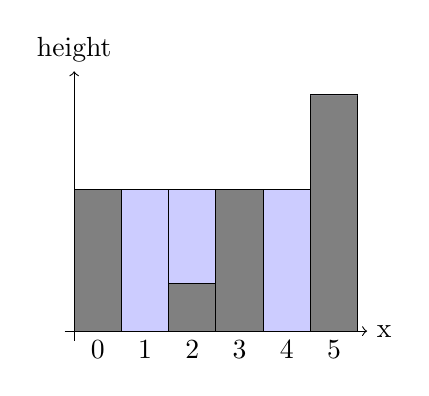
\begin{tikzpicture}[scale=0.6]
  % Data: index/height/water
  \foreach \i/\h/\w in {
    0/3/0,
    1/0/3,
    2/1/2,
    3/3/0,
    4/0/3,
    5/5/0} {
    % draw bar
    \draw[fill=black!50] (\i,0) rectangle ++(1,\h);
    % draw water (height \w) on top of bar
    \draw[fill=blue!20] (\i,\h) rectangle ++(1,\w);
  }
  % axes
  \draw[->] (-0.2,0) -- (6.2,0) node[right] {x};
  \draw[->] (0,-0.2) -- (0,5.5) node[above] {height};
  % x labels
  \foreach \i in {0,...,5}
    \node[below] at (\i+0.5,0) {\i};
\end{tikzpicture}

\begin{minted}[
    bgcolor=bgcolor2,
    frame=lines,
    framesep=5mm,
    rulecolor=\color{black},
    linenos,
    numbersep=5pt,
    fontsize=\normalsize
]{python}
def trap_rain_water(height: List[int]) -> int:
    """
    Calculates the amount of rain water that can be trapped between bars.
    Uses a two-pointer approach which is space-efficient.
    Time Complexity: O(n), Space: O(1)
    """    
    # If fewer than 3 bars, no “bucket” can form see pic for clarity water stored over bar
    if not height or len(height) < 3:
        return 0
    left, right = 0, len(height) - 1
    left_max, right_max = 0, 0
    water_trapped = 0

    while left < right:
        if height[left] < height[right]:
            # Water level determined by left side, move left pointer
            if height[left] >= left_max:
                left_max = height[left]
            else:
                water_trapped += left_max - height[left]
            left += 1
        else:
            # Water level determined by right side, move right pointer
            if height[right] >= right_max:
                right_max = height[right]
            else:
                water_trapped += right_max - height[right]
            right -= 1
            
    return water_trapped
\end{minted}

\noindent\textbf{Problem: Minimum Consecutive Flips}
\begin{minted}[
    bgcolor=bgcolor3,
    frame=lines,
    framesep=5mm,
    rulecolor=\color{black},
    linenos,
    numbersep=5pt,
    fontsize=\normalsize
]{python}
def min_consecutive_flips(binary_array: List[int]) -> int:
    """
    Finds the minimum number of flips needed to make all elements in a
    binary array the same (all 0s or all 1s). A flip changes a contiguous block.
    This is achieved by counting alternating groups and choosing the minimum.
    Time Complexity: O(n), Space: O(1)
    """
    if not binary_array:
        return 0
    
    num_zeros_blocks = 0
    num_ones_blocks = 0

    # Initialize counts for the first block
    if binary_array[0] == 0:
        num_zeros_blocks = 1
    else:
        num_ones_blocks = 1

    # Iterate through the array to find transitions and count blocks
    for i in range(1, len(binary_array)):
        if binary_array[i] != binary_array[i-1]:
            if binary_array[i] == 0:
                num_zeros_blocks += 1
            else:
                num_ones_blocks += 1
    
    # The minimum flips required is the smaller count of blocks.
    # For example, if you have '0011100', blocks are (00, 111, 00).
    # Zero blocks: 2. One blocks: 1. Min is 1 (flip '111' to make all 0s).
    return min(num_zeros_blocks, num_ones_blocks)
\end{minted}

\noindent\textbf{Problem: Sliding Window Technique (Example: Max Sum Subarray of Size K)}
\begin{minted}[
    bgcolor=bgcolor4,
    frame=lines,
    framesep=5mm,
    rulecolor=\color{black},
    linenos,
    numbersep=5pt,
    fontsize=\normalsize
]{python}
def max_sum_subarray_of_size_k(nums: List[int], k: int) -> int:
    """
    Finds the maximum sum of a subarray of a fixed size K using the sliding window technique. [5]
    Time Complexity: O(n), Space: O(1)
    """
    if k <= 0 or not nums or k > len(nums):
        return 0 # Or raise error, based on problem specific constraints
    
    current_window_sum = 0
    
    # Calculate sum of the first window (size k)
    for i in range(k):
        current_window_sum += nums[i]
    
    max_window_sum = current_window_sum
    
    # Slide the window across the array
    for i in range(k, len(nums)):
        current_window_sum += nums[i] - nums[i - k] # Add new element, subtract old element
        max_window_sum = max(max_window_sum, current_window_sum)
        
    return max_window_sum
\end{minted}

\noindent\textbf{Problem: Consecutive Ones III (Max Consecutive Ones with K Flips)}
\begin{minted}[
    bgcolor=bgcolor5,
    frame=lines,
    framesep=5mm,
    rulecolor=\color{black},
    linenos,
    numbersep=5pt,
    fontsize=\normalsize
]{python}
def longest_ones(nums: List[int], k: int) -> int:
    """
    Given a binary array nums and an integer k, return the maximum number of
    consecutive 1's in the array if you can flip at most k 0's.
    This uses a sliding window where the window expands and shrinks based on zero count.
    Time Complexity: O(n) 2*n traversal by right and left , Space: O(1)
    """
    left = 0
    zero_count = 0
    max_length = 0

    for right in range(len(nums)):
        if nums[right] == 0:
            zero_count += 1
        
        # If zero_count exceeds k, shrink the window from the left by moving 'left' pointer
        while zero_count > k:
            if nums[left] == 0: # If the element leaving the window is a zero, decrement zero_count
                zero_count -= 1
            left += 1
        
        # Update max_length for the current valid window
        max_length = max(max_length, right - left + 1)
        
    return max_length
\end{minted}
\noindent\textbf{Problem: Max Consecutive Ones with K Flips (Strictly single traversal) }
\begin{minted}[
    bgcolor=bgcolor5,
    frame=lines,
    framesep=5mm,
    rulecolor=\color{black},
    linenos,
    numbersep=5pt,
    fontsize=\normalsize
]{python}
def longest_ones(nums: List[int], k: int) -> int:
    """
    Given a binary array nums and an integer k, return the maximum number of
    consecutive 1's in the array if you can flip at most k 0's.
    This uses a sliding window where the window expands and shrinks based on zero count. 
    Time Complexity: O(n) Strictly single traversal , Space: O(1)
    """
    left ,zc ,max_len = 0 ,0 ,0
      for right in range(len(nums)):
        # 1) Expand window to include nums[right]
        if nums[right] == 0:
            zc += 1

        # 2) If too many zeros, shrink from the left until zc <= k
        if zc > k:
            # If the element at `left` was a flipped‐zero, un‐flip it
            if nums[left] == 0:
                zc -= 1
            left += 1

        # 3) Now window [left..right] has <= k zeros: record its size
        #    We only update when it's valid; this guarantees max_len always
        #    reflects a window we could actually achieve by flipping <= k zeros.
        if zc <= k:
            max_len = max(max_len, right - left + 1)

    return max_len

\end{minted}
\noindent\textbf{Problem: Longest Substring with At Most K Distinct Characters}
\begin{minted}[
    bgcolor=bgcolor6,
    frame=lines,
    framesep=5mm,
    rulecolor=\color{black},
    linenos,
    numbersep=5pt,
    fontsize=\normalsize
]{python}


def longest_substring_k_distinct(s: str, k: int) -> int:
    """
    Finds the length of the longest substring with at most K distinct characters.
    This is analogous to the "Fruit in Basket" problem. 
    Uses a sliding window with a hash map for frequency tracking. 
    Time Complexity: O(n), Space: O(k) (for the frequency map, max k distinct chars)
    """
    if k == 0:
        return 0
    
    char_freq: Dict[str, int] = {}
    left = 0
    max_length = 0

    for right in range(len(s)):
        char_freq[s[right]] = char_freq.get(s[right], 0) + 1
        
        # Shrink the window from the left if distinct characters exceed k
        while len(char_freq) > k:
            char_freq[s[left]] -= 1
            if char_freq[s[left]] == 0: # If count becomes 0, remove char from map
                del char_freq[s[left]]
            left += 1
        
        # Update max_length for the current valid window
        max_length = max(max_length, right - left + 1)
        
    return max_length

    # Can easily converted it to above strictly O(N) by replacing while with if
    #And checking the size of map before updating max_length .!Just this much


    ###########################ALTERNATE IMPLEMENTATION########################

def longest_substring_k_distinct(s: str, k: int) -> int:
    """
    Longest substring with at most k distinct characters.
    Time: O(n), Space: O(k)
    """
    if k == 0 or not s:
        return 0

    left = 0
    max_len = 0
    # char → last index seen; insertion order = window order
    window: "OrderedDict[str,int]" = OrderedDict()

    for right, ch in enumerate(s):
        # If ch already in window, delete+reinsert to update its “recentness”
        if ch in window:
            del window[ch]
        window[ch] = right

        # If we now have > k distinct, evict the oldest:
        if len(window) > k:
            # popitem(last=False) removes the first key inserted
            old_char, old_index = window.popitem(last=False)
            # move left pointer just beyond that char’s last occurrence
            left = old_index + 1

        # window is valid: [left..right] contains <= k distinct characters
        max_len = max(max_len, right - left + 1)

    return max_len

\end{minted}

\noindent\textbf{Problem: Longest Substring Without Repeating Characters}
\begin{minted}[
    bgcolor=bgcolor7,
    frame=lines,
    framesep=5mm,
    rulecolor=\color{black},
    linenos,
    numbersep=5pt,
    fontsize=\normalsize
]{python}
def length_of_longest_substring(s: str) -> int:
    """
    Finds the length of the longest substring without repeating characters.
    Uses a sliding window with a map to track the last seen index of characters. 
    Time Complexity: O(n), Space: O(alphabet_size) (for the character index map)
    """
    char_index_map: Dict[str, int] = {} # Stores char -> its last seen index
    left = 0
    max_length = 0

    for right in range(len(s)):
        current_char = s[right]
        
        # If current_char is already in the map AND its last seen index
        # is within the current window (i.e., char_index_map[current_char] >= left),
        # then move the left pointer to avoid the repeating character.
        if current_char in char_index_map and char_index_map[current_char] >= left:
            left = char_index_map[current_char] + 1
        
        char_index_map[current_char] = right # Update last seen index of current_char
        max_length = max(max_length, right - left + 1)
        
    return max_length
\end{minted}

\noindent\textbf{Problem: Sub array sum = K for array containing positives, zero and negatives}
\begin{minted}[
    bgcolor=bgcolor8,
    frame=lines,
    framesep=5mm,
    rulecolor=\color{black},
    linenos,
    numbersep=5pt,
    fontsize=\normalsize
]{python}
def subarray_sum_equals_k(nums: List[int], k: int) -> int:
    """
    Returns the number of contiguous subarrays whose sum == k.
    Handles negative numbers—sliding window won’t work here.
    Time: O(n), Space: O(n)
    """
    count = 0
    prefix_sum = 0
    # Map from prefix_sum value to how many times we've seen it so far.
    # We seed with {0:1} so that any prefix_sum == k at index i counts as a valid subarray [0..i].
    seen: Dict[int,int] = {0: 1}

    for x in nums:
        prefix_sum += x
        # If (prefix_sum - k) appeared before, those are subarrays ending here summing to k
        if (prefix_sum - k) in seen:
            count += seen[prefix_sum - k]

        # Record this prefix_sum for future subarrays
        seen[prefix_sum] = seen.get(prefix_sum, 0) + 1

    return count
    ####   Apply Same for Binary Subarray with sum S
\end{minted}
\noindent\textbf{Problem: Zero Containg subarray with sum K(Binary Subarray ) }
\begin{minted}[
    bgcolor=bgcolor8,
    frame=lines,
    framesep=5mm,
    rulecolor=\color{black},
    linenos,
    numbersep=5pt,
    fontsize=\normalsize
]{python}
def subarray_sum_equals_k(nums: List[int], k: int) -> int:
    """
    Returns the number of contiguous subarrays whose sum == k.
    This can't handle negatives!!!
    Time: O(n), Space: O(n)
    """
    def numSubarraysWithSum(nums, k):
        def atMost(s):
            if s < 0:
                return 0
            left = 0
            count = 0
            curr_sum = 0
            for right in range(len(nums)):
                curr_sum += nums[right]
                while curr_sum > s:
                    curr_sum -= nums[left]
                    left += 1
                count += right - left + 1
            return count

    return atMost(k) - atMost(k - 1)   
    ####   Apply Same for Binary Subarray with sum S
\end{minted}
\noindent\textbf{Problem: Count All Substrings With Exactly K Distinct Characters}
\begin{minted}[
    bgcolor=bgcolor9,
    frame=lines,
    framesep=5mm,
    rulecolor=\color{black},
    linenos,
    numbersep=5pt,
    fontsize=\normalsize
]{python}


def _at_most_k_distinct_substrings(s: str, k: int) -> int:
    """
    Helper function to count substrings with at most K distinct characters.
    Time Complexity: O(n), Space: O(alphabet_size)
    """
    if k < 0: # No substrings can have negative distinct characters
        return 0
    if k == 0: # Only empty string or no distinct characters, usually 0 substrings
        return 0

    char_freq: Dict[str, int] = {}
    left = 0
    count = 0

    for right in range(len(s)):
        char_freq[s[right]] = char_freq.get(s[right], 0) + 1
        
        while len(char_freq) > k:
            char_freq[s[left]] -= 1
            if char_freq[s[left]] == 0:
                del char_freq[s[left]]
            left += 1
        
        # All substrings ending at 'right' and starting from 'left' up to 'right'
        # have at most k distinct characters. The count is the length of the current window.
        count += (right - left + 1)
        
    return count

def count_exactly_k_distinct_substrings(s: str, k: int) -> int:
    """
    Counts the number of substrings with exactly K distinct characters.
    Uses the principle: count(exactly K) = count(at most K) - count(at most K-1). 
    Time Complexity: O(n), Space: O(alphabet_size)
    """
    return _at_most_k_distinct_substrings(s, k) - _at_most_k_distinct_substrings(s, k - 1)
    #Because using 2 pointers we cant take in account for abbbbbccdce k=3 
    #Lots of correct windows are skipped due to incrementing r for exact matching
\end{minted}

\noindent\textbf{Problem: Print All Substrings With Exactly K Distinct Characters}
\begin{minted}[
    bgcolor=bgcolor10,
    frame=lines,
    framesep=5mm,
    rulecolor=\color{black},
    linenos,
    numbersep=5pt,
    fontsize=\normalsize
]{python}
from typing import List, Dict

def print_exactly_k_distinct_substrings(s: str, k: int) -> List[str]:
    """
    Prints all substrings with exactly K distinct characters.
    It iterates through all possible start and end points of substrings. 
    Time Complexity: O(n^2 * alphabet_size) (due to nested loops and map operations)
    Space Complexity: O(alphabet_size) (for the frequency map)
    """
    result_substrings: List[str] = []
    n = len(s)

    for i in range(n): # Start of substring
        char_freq: Dict[str, int] = {}
        distinct_count = 0
        for j in range(i, n): # End of substring
            char = s[j]
            if char_freq.get(char, 0) == 0: # New distinct character found
                distinct_count += 1
            char_freq[char] = char_freq.get(char, 0) + 1
            
            if distinct_count == k:
                result_substrings.append(s[i:j+1])
            elif distinct_count > k:
                # Optimization: If distinct count exceeds k, no further substrings
                # starting at 'i' will have exactly k distinct characters by extending.
                break 
    return result_substrings
\end{minted}

\noindent\textbf{Problem: Prefix Sum Technique (Example: Range Sum Query)}
\begin{minted}[
    bgcolor=bgcolor1,
    frame=lines,
    framesep=5mm,
    rulecolor=\color{black},
    linenos,
    numbersep=5pt,
    fontsize=\normalsize
]{python}
class PrefixSumArray:
    """
    Implements the prefix sum technique for efficient range sum queries.
    Preprocessing Time Complexity: O(n)
    Query Time Complexity: O(1) [8]
    Space Complexity: O(n)
    """
    def __init__(self, nums: List[int]):
        # Build prefix sum array [7]
        self.prefix_sum =  * (len(nums) + 1)
        for i in range(len(nums)):
            self.prefix_sum[i+1] = self.prefix_sum[i] + nums[i]
            
    def query_range_sum(self, start_idx: int, end_idx: int) -> int:
        """
        Returns the sum of elements in the range [start_idx, end_idx] (inclusive).
        Assumes 0-based indexing for input array.
        """
        if not (0 <= start_idx <= end_idx < len(self.prefix_sum) - 1):
            raise IndexError("Invalid range indices")
        
        return self.prefix_sum[end_idx + 1] - self.prefix_sum[start_idx]
\end{minted}

\noindent\textbf{Problem: Maximum Appearing Element in Ranges (Line Sweep)}
\begin{minted}[
    bgcolor=bgcolor2,
    frame=lines,
    framesep=5mm,
    rulecolor=\color{black},
    linenos,
    numbersep=5pt,
    fontsize=\normalsize
]{python}
def max_appearing_element_in_ranges(L: List[int], R: List[int]) -> int:
    """
    Finds the element that appears maximum number of times across given ranges [L[i], R[i]].
    Uses a difference array and then computes prefix sums to find the maximum.
    Time Complexity: O(N + max_val), where N is number of ranges, max_val is max R[i].
    Space Complexity: O(max_val)
    """
    if not L or not R or len(L) != len(R):
        return -1 # Handle invalid input
    
    max_range_val = 0
    if R:
        max_range_val = max(R)

    # Create a difference array. Size max_range_val + 2 to handle R[i]+1.
    # If values can be very large, coordinate compression might be needed.
    freq_arr =  * (max_range_val + 2) 

    for i in range(len(L)):
        freq_arr[L[i]] += 1
        freq_arr[R[i] + 1] -= 1
    
    max_frequency = 0
    result_element = -1
    current_frequency = 0

    # Compute prefix sums on the difference array to get actual frequencies
    for i in range(max_range_val + 1):
        current_frequency += freq_arr[i]
        if current_frequency > max_frequency:
            max_frequency = current_frequency
            result_element = i
            
    return result_element
\end{minted}

\noindent\textbf{Problem: Subarray with Given Sum (Count)}
\begin{minted}[
    bgcolor=bgcolor3,
    frame=lines,
    framesep=5mm,
    rulecolor=\color{black},
    linenos,
    numbersep=5pt,
    fontsize=\normalsize
]{python}
def count_subarrays_with_sum_k(nums: List[int], k: int) -> int:
    """
    Count how many contiguous subarrays of a positive-only array sum exactly to k.
    Time: O(n), Space: O(1)
    """
    count = 0
    curr_sum = 0
    left = 0

    for right, v in enumerate(nums):
        # 1) Extend window to the right
        curr_sum += v

        # 2) Shrink from the left until sum <= k
        #    (valid because every element >= 0)
        while curr_sum > k and left <= right:
            curr_sum -= nums[left]
            left += 1

        # 3) If we hit exactly k, that window [left..right] is one match
        if curr_sum == k:
            count += 1

    return count
    # For calculating longest such similiar code. 
    ####################################################################################
def subarray_sum_count(nums: List[int], target_sum: int) -> int:
    """
    Counts the number of subarrays that sum up to a specific target_sum.
    Works for arrays with positive, negative, and zero integers using prefix sums and a hash map. 
    Time Complexity: O(n), Space: O(n) (for the prefix sum map)
    """
    # prefix_sums_freq: maps a prefix sum to its frequency
    prefix_sums_freq: Dict[int, int] = {0: 1} # Initialize with 0 sum occurring once (empty prefix)
    current_sum = 0
    count = 0

    for num in nums:
        current_sum += num
        # If (current_sum - target_sum) exists in the map,
        # it means there's a previous prefix sum that, when subtracted
        # from the current_sum, results in target_sum.
        count += prefix_sums_freq.get(current_sum - target_sum, 0)
        
        # Add the current_sum to the map, incrementing its frequency
        prefix_sums_freq[current_sum] = prefix_sums_freq.get(current_sum, 0) + 1
        
    return count
\end{minted}

\noindent\textbf{Problem: Next Permutation}
\begin{minted}[
    bgcolor=bgcolor4,
    frame=lines,
    framesep=5mm,
    rulecolor=\color{black},
    linenos,
    numbersep=5pt,
    fontsize=\normalsize
]{python}
def next_permutation(nums: List[int]) -> None:
    """
    Rearranges numbers into the lexicographically next greater permutation.
    It involves finding the longest non-increasing suffix, swapping a pivot, and reversing.
    Time Complexity: O(n), Space: O(1)
    """
    n = len(nums)
    
    # 1. Find the largest index k such that nums[k] < nums[k+1]
    # This identifies the "pivot" point to change the permutation.
    k = -1
    for i in range(n - 2, -1, -1):
        if nums[i] < nums[i+1]:
            k = i
            break
    
    if k == -1: # If no such index exists, the permutation is the last permutation
        nums.reverse() # In this case, reverse the entire array to get the first permutation.
        return

    # 2. Find the largest index l greater than k such that nums[k] < nums[l]
    # This finds the smallest element in the suffix that is greater than nums[k].
    l = -1
    for i in range(n - 1, k, -1):
        if nums[i] > nums[k]:
            l = i
            break
            
    # 3. Swap nums[k] and nums[l]
    nums[k], nums[l] = nums[l], nums[k]
    
    # 4. Reverse the subarray from index k+1 to the end
    # This sorts the suffix in non-decreasing order, making it the lexicographically smallest.
    left, right = k + 1, n - 1
    while left < right:
        nums[left], nums[right] = nums[right], nums[left]
        left += 1
        right -= 1
\end{minted}

\noindent\textbf{Problem: Maximum Product Subarray}
\begin{minted}[
    bgcolor=bgcolor5,
    frame=lines,
    framesep=5mm,
    rulecolor=\color{black},
    linenos,
    numbersep=5pt,
    fontsize=\normalsize
]{python}
def max_product_subarray(nums: List[int]) -> int:
    """
    Finds the maximum product of a contiguous non-empty subarray within an array.
    It tracks current maximum and minimum products due to negative numbers.
    Time Complexity: O(n), Space: O(1)
    """
    if not nums:
        return 0

    max_so_far = nums # Stores the maximum product ending at current index
    min_so_far = nums # Stores the minimum product ending at current index
    result = nums     # Stores the overall maximum product found

    for i in range(1, len(nums)):
        curr = nums[i]
        
        # When current number is negative, max_so_far and min_so_far swap roles
        if curr < 0:
            max_so_far, min_so_far = min_so_far, max_so_far
        
        # Update max_so_far and min_so_far for the current index
        max_so_far = max(curr, max_so_far * curr)
        min_so_far = min(curr, min_so_far * curr)
        
        # Update the overall result
        result = max(result, max_so_far)
        
    return result
    ###########################ALTERNATE IMPLEMENTATION########################
    # Idea is to remove just one negative incase of odd negatives otherwise whole array is answer
    def max_product_subarray(nums: List[int]) -> int:
    """Take in account zeros also by maintaining two pointers
    Time Complexity: O(n), Space: O(1)"""
    prefix , suffix = 1 , 1
    ans = -math.inf
    for i in range(len(nums)) :
        if prefix == 0:
            prefix =1
        if suffix ==0 :
            suffix =1
        prefix *= nums[i]
        suffix *= nums[lens(nums) - i -1]
        ans = min(ans , prefix , suffix)

    return ans

\end{minted}

\noindent\textbf{Problem: Find Rotation Count (Sorted and Rotated Array)}
\begin{minted}[
    bgcolor=bgcolor6,
    frame=lines,
    framesep=5mm,
    rulecolor=\color{black},
    linenos,
    numbersep=5pt,
    fontsize=\normalsize
]{python}
def find_rotation_count(nums: List[int]) -> int:
    """
    Finds the number of times a sorted array has been rotated.
    This is equivalent to finding the index of the minimum element using binary search. [9]
    Time Complexity: O(log n), Space: O(1)
    """
    n = len(nums)
    if n == 0:
        return 0
    
    low, high = 0, n - 1
    
    while low <= high:
        # If the subarray is already sorted (no rotation in this segment),
        # or if only one element is left, then nums[low] is the minimum.
        if nums[low] <= nums[high]:
            return low # The minimum element's index is the rotation count.

        mid = low + (high - low) // 2
        
        # Calculate indices for next and previous elements circularly
        next_idx = (mid + 1) % n 
        prev_idx = (mid - 1 + n) % n 

        # If mid element is smaller than or equal to its neighbors, it's the minimum element.
        if nums[mid] <= nums[prev_idx] and nums[mid] <= nums[next_idx]:
            return mid
        
        # Decide which half to search based on which half is sorted
        if nums[mid] <= nums[high]: # Right half is sorted, minimum must be in the left half
            high = mid - 1
        else: # Left half is sorted, minimum must be in the right half
            low = mid + 1
            
    return 0 # Should ideally not be reached if array is sorted and rotated
\end{minted}
\noindent\textbf{Problem: Minimumm Window Substring }
\begin{minted}[
    bgcolor=bgcolor6,
    frame=lines,
    framesep=5mm,
    rulecolor=\color{black},
    linenos,
    numbersep=5pt,
    fontsize=\normalsize
]{python}
def min_window(s: str, t: str) -> str:
    """
    Return the smallest substring of s that contains every character of t (including duplicates).
    If no such window exists, return the empty string.
    Time: O(|s| + |t|), Space: O(|s| + |t|)
    """
    if not t or not s:
        return ""

    need = Counter(t)            # counts of chars we need
    window = {}                  # counts of chars in the current window
    required = len(need)         # how many distinct chars we must fully match
    formed = 0                   # how many distinct chars currently meet their need

    l = 0                        # left pointer of our window
    ans = (float("inf"), None, None)  # (window length, left, right)

    # Expand the window by moving r
    for r, ch in enumerate(s):
        window[ch] = window.get(ch, 0) + 1
        # If this char is one we care about and we've hit its required count
        if ch in need and window[ch] == need[ch]:
            formed += 1

        # When we've formed a valid window, try to shrink it from the left
        while l <= r and formed == required:
            # Update our answer if this window is smaller
            if (r - l + 1) < ans[0]:
                ans = (r - l + 1, l, r)

            # Pop the leftmost character out of the window
            left_char = s[l]
            window[left_char] -= 1
            if left_char in need and window[left_char] < need[left_char]:
                formed -= 1

            l += 1  # shrink from the left

    return "" if ans[0] == float("inf") else s[ans[1] : ans[2] + 1]

\end{minted}
% \end{document}

\newgeometry{margin=0.2in}
\vspace*{47mm}

\begin{center}

{\fontsize{55}{20}\selectfont \textcolor{headingcolor}{\bfseries SEARCHES}}
\end{center}

\vspace{50mm}

\begin{center}

\includegraphics[height=13.88cm, width=17cm, keepaspectratio]{Pics/search.png}
\end{center}

\chapter{Essential Binary Search Techniques  }
\phantomsection                      % <-- creates a hyperlink anchor
\label{sec:search}
\begin{itemize}
    \item \textbf{Standard Binary Search Pattern:}
    \begin{itemize}
        \item Initialize \texttt{left} and \texttt{right} boundaries
        \item While \texttt{left <= right}: 
        \item \quad Calculate \texttt{mid = left + (right - left) // 2} (prevents overflow)
        \item \quad Three-way comparison: 
        \begin{itemize}
            \item Equal: return \texttt{mid}
            \item Target $<$ \texttt{arr[mid]}: \texttt{right = mid - 1}
            \item Target $>$ \texttt{arr[mid]}: \texttt{left = mid + 1}
        \end{itemize}
    \end{itemize}
    
    \item \textbf{Search Space Selection:}
    \begin{itemize}
        \item Sorted arrays (obvious case)
        \item Answer prediction: When answer space is monotonic (min/max problems)
        \item Function domains: Where f(x) transitions from false to true
    \end{itemize}
    
    \item \textbf{Lower/Upper Bound Variants:}
    \begin{itemize}
        \item First occurrence: When \texttt{arr[mid] == target}, set \texttt{right = mid - 1}
        \item Last occurrence: When \texttt{arr[mid] == target}, set \texttt{left = mid + 1}
        \item Floor: Largest element $\leq$ target
        \item Ceil: Smallest element $\geq$ target
    \end{itemize}
    
    \item \textbf{Rotated Array Searches:}
    \begin{itemize}
        \item Find pivot: Compare \texttt{arr[mid]} with \texttt{arr[0]} or \texttt{arr[high]}
        \item Two-pass: Find pivot then binary search in segment
        \item Single-pass: Check which segment is sorted
    \end{itemize}
    
    \item \textbf{Matrix Searches:}
    \begin{itemize}
        \item Row-sorted + column-sorted: Start from top-right corner
        \item Convert 2D to 1D: \texttt{mid} to \texttt{(mid//cols, mid\%cols)}
        \item Find k-th smallest: Binary search on value range
    \end{itemize}
    
    \item \textbf{Answer Prediction Patterns:}
    \begin{itemize}
        \item Minimize maximum: "Split array largest sum", "ship packages"
        \item Maximize minimum: "Aggressive cows", "max distance to gas station"
        \item Condition-based: First value where condition becomes true
    \end{itemize}
    
    \item \textbf{Bitonic Array Searches:}
    \begin{itemize}
        \item Find peak: Compare \texttt{arr[mid]} with neighbors
        \item Ascending segment: Standard binary search
        \item Descending segment: Reverse binary search logic
    \end{itemize}
    
    \item \textbf{Advanced Applications:}
    \begin{itemize}
        \item Real number domains: Precision handling with tolerance
        \item Binary search on function: Square root, monotonic functions
        \item Exponential search: For unbounded arrays
    \end{itemize}
    
    \item \textbf{Decision Function Design:}
    \begin{itemize}
        \item Must be monotonic: \texttt{f(x)} transitions once from false to true
        \item Efficient implementation: O(n) or better
        \item Parameterization: Often requires additional parameters (k, limit)
    \end{itemize}
    
    \item \textbf{Termination Conditions:}
    \begin{itemize}
        \item Standard: \texttt{while (left <= right)}
        \item Alternative: \texttt{while (left < right)} with \texttt{left = mid + 1} or \texttt{right = mid}
        \item Exact match vs. closest value
    \end{itemize}
    
    \item \textbf{Edge Cases:}
    \begin{itemize}
        \item Empty arrays
        \item Single-element arrays
        \item All elements equal
        \item Target outside range
        \item Duplicate elements
        \item Integer overflow in \texttt{mid} calculation
    \end{itemize}
    
    \item \textbf{Optimization Tricks:}
    \begin{itemize}
        \item Precomputation: For decision functions
        \item Early termination: When possible
        \item Two-layer binary search: Value + position
        \item Sanity checks: Before starting search
    \end{itemize}
    
    \item \textbf{Common Problem Patterns:}
    \begin{itemize}
        \item Search in infinite stream: Exponential + binary search
        \item Find missing element: Compare index vs value
        \item Find rotation count: Pivot index
        \item Find peak element: Local maxima
    \end{itemize}
    
    \item \textbf{Debugging Tips:}
    \begin{itemize}
        \item Print \texttt{left/mid/right} values
        \item Check loop invariants
        \item Test with small cases (n=0,1,2,3)
        \item Verify decision function logic
    \end{itemize}
    
    \item \textbf{Alternative Implementations:}
    \begin{itemize}
        \item Bisect module in Python
        \item \texttt{std::lower\_bound} in C++
        \item \texttt{Arrays.binarySearch} in Java
        \item Custom comparators
    \end{itemize}
\end{itemize}
\section{Search-Based DSA Problems Summary Table}
\begin{longtable}{|>{\raggedright\arraybackslash}p{3.2cm}|>{\columncolor{c2}\centering\arraybackslash}p{2.5cm}|>{\columncolor{c3}\raggedright\arraybackslash}p{4.3cm}|>{\columncolor{c4}\raggedright\arraybackslash}p{3.5cm}|>{\columncolor{c5}\color{white}\raggedright\arraybackslash}p{3.5cm}|}
\hline
\rowcolor{rclr}
\textbf{Problem Name} & \textbf{Time Complexity} & \textbf{Idea to Solve} & \textbf{Optimization Tip} & \textbf{Edge Cases} \\
\hline
\endfirsthead
\hline
\rowcolor{rclr}
\textbf{Problem Name} & \textbf{Time Complexity} & \textbf{Idea to Solve} & \textbf{Optimization Tip} & \textbf{Edge Cases} \\
\hline
\endhead
\hline
Ternary Search & $\mathcal{O}(\log n)$ & Divide range in 3 parts, recursively reduce search space. & Prefer over binary only in unimodal functions. & Non-unimodal function \\
\hline
Jump Search & $\mathcal{O}(\sqrt{n})$ & Jump by fixed step, then linear search in block. & Best for uniformly distributed sorted data. & Element near start or end \\
\hline
Missing and Repeating Number & $\mathcal{O}(n)$ & Use sum and sum of squares formula to derive two equations and solve for missing and repeating. & Use integer overflow-safe formulas or XOR-based approach. & Duplicates at start/end, all same elements \\
\hline
Find Peak Element in Unsorted Array & $\mathcal{O}(\log n)$ & Apply binary search: if mid $>$ neighbors, it's a peak, else move in direction of greater neighbor. & Avoid linear scan by using binary search. & Peak at boundaries, flat plateau \\
\hline
Search in an Infinite Sized Array & $\mathcal{O}(\log n)$ & Exponentially expand range until element $>$ target, then binary search in found range. & Start with small window and double size to minimize search space. & Very large target, target not present \\
\hline
Median of Two Sorted Arrays & $\mathcal{O}(\log \min(n, m))$ & Binary search on smaller array to partition both arrays at correct position. & Always binary search on smaller array to ensure log(min(n,m)). & Odd total length, one array empty \\
\hline

Search in Sorted Rotated Array & $\mathcal{O}(\log n)$ but $\mathcal{O}(n)$ for duplicates & Modified binary search: identify sorted half, move accordingly. & For same low, mid, high keep l++,h-- until not equal. & Rotation at 0 or n-1, duplicates at low,mid,high (for generalized) \\
\hline
Find Triplet with Given Sum (sorted) & $\mathcal{O}(n^2)$ & Fix one element and apply two-pointer approach on the rest. & Sort array once before outer loop. & No triplet found, multiple same triplets \\
\hline
One Repeating Element in Array from 1 to N (size N) & $\mathcal{O}(n)$ & Use Floyd’s Cycle Detection or array marking. & Prefer Floyd’s for O(1) space. & Repetition at start or end, minimal repeat count \\
\hline
One Repeating Element in Array from 1 to N (size N) & $\mathcal{O}(n)$ & Take $\Sigma n - \Sigma a[i] -eq(i) \space \& \space  
\Sigma n^2 - \Sigma a[i]^2 - eq(ii)$. & $Xor(a[i]) with Xor(1 .. n)$ then find different bit and proceed like 2 odd appearing. & Repetition at start or end, minimal repeat count \\
\hline
Multiple Repeating Elements in Array from 1 to N (size N) & $\mathcal{O}(n)$ & Use frequency count or mark visited indices using negation or add N. & Use modulo trick to track frequency in-place. & All elements same, no repetition \\
\hline
Allocate Minimum Pages(Similiar to Painter's partition or Split subarray minimum largest sum) & $O(n \cdot \log(sum(pages)$ & Binary search on answer in range max\_element to sum(array)+ greedy check if allocation is feasible with mid pages & Minimize max load among partitions & Pages $>$ total or students $>$ books \\
\hline
Minimum Days to Make $n$ Bouquets & $O(n \log D)$ & Binary search on days; check if $\geq n$ bouquets possible by checking $k$ adjacent bloom days $\leq mid$ & Greedy simulation inside binary search & Not enough flowers \\
\hline
Capacity to Ship Packages in D Days & $O(n \log \sum)$ & Binary search on capacity; check if packages can be shipped within $D$ days & Use greedy validation per capacity guess & Package weight > mid \\
\hline
Aggressive Cows & $O(n \log d)$ & Binary search on distance; place cows greedily with min gap $\geq mid$ & Sort stalls before processing & Only one cow or all cows = stalls \\
\hline
Kth Missing Positive Number & $O(\log n)$ & Binary search: $arr[i] - i - 1$ gives count of missing up to $i$ & Use linear scan if $n$ small & k before first element \\
\hline
Kth Element in Two Sorted Arrays & $O(\log \min(n, m))$ & Partition both arrays such that left parts have $k$ elements; binary search on smaller array & Handle all partition edge cases (0, n) & k = 1 or k = total length \\
\hline
Longest Repeating Substring (Binary Search) & $O(n \log n)$ & Binary search on length + rolling hash/set to check duplicates & Rabin-Karp-style hashing or Trie for checking repetition & Same substrings at different positions \\
\hline
\end{longtable}
\clearpage
\newgeometry{margin=1in}
\input{solutions/binary_sear}
\newgeometry{margin=0.2in}
\vspace*{47mm}

\begin{center}

{\fontsize{55}{20}\selectfont \textcolor{headingcolor}{\bfseries MATRIX}}
\end{center}

\vspace{50mm}

\begin{center}

\includegraphics[height=13.88cm, width=17cm, keepaspectratio]{Pics/matrix.png}
\end{center}

\chapter{Essential Matrix Techniques  }
\phantomsection                      % <-- creates a hyperlink anchor
\label{sec:matrix}
\begin{itemize}
    \item \textbf{Matrix Traversal Fundamentals:}
    \begin{itemize}
        \item Directions handling: Define \texttt{dirs = [(0,1), (1,0), (0,-1), (-1,0)]} for 4-way, add diagonals for 8-way
        \item Boundary checks: Verify \texttt{0 <= x < m} and \texttt{0 <= y < n} before accessing
        \item Visited tracking: Use visited matrix or in-place modification (mark as \#' or \texttt{-1})
    \end{itemize}
    
    \item \textbf{Breadth-First Search (BFS) Patterns:}
    \begin{itemize}
        \item Shortest path in unweighted grid:
        \begin{itemize}
            \item Multi-source BFS: Initialize queue with all starting points (e.g., rotting oranges)
            \item Layer tracking: Use queue size for level-order traversal
        \end{itemize}
        \item Flood fill variants: 
        \begin{itemize}
            \item Connected component counting (islands)
            \item Boundary detection (enclosed regions)
        \end{itemize}
        \item Optimization: 
        \begin{itemize}
            \item Bidirectional BFS for single-target paths
            \item Early termination when target found
        \end{itemize}
    \end{itemize}
    
    \item \textbf{Depth-First Search (DFS) \& Recursion:}
    \begin{itemize}
        \item Connected components: 
        \begin{itemize}
            \item Standard DFS: Mark visited during recursion
            \item Count size/mark islands
        \end{itemize}
        \item Pathfinding with backtracking: 
        \begin{itemize}
            \item Explore all paths (rat in a maze)
            \item Prune invalid paths early
        \end{itemize}
        \item Cycle detection: 
        \begin{itemize}
            \item Track recursion stack with \texttt{visiting} state
            \item Detect in directed graphs (dependency matrices)
        \end{itemize}
        \item Optimization:
        \begin{itemize}
            \item Memoization: Cache states when possible
            \item Iterative DFS to avoid stack overflow
        \end{itemize}
    \end{itemize}
    
    \item \textbf{Dynamic Programming on Matrices:}
    \begin{itemize}
        \item Path counting: 
        \begin{itemize}
            \item \texttt{dp[i][j] = dp[i-1][j] + dp[i][j-1]} (right/down moves)
            \item Handle obstacles: Set \texttt{dp[i][j] = 0} at blocked cells
        \end{itemize}
        \item Minimum path sum: 
        \begin{itemize}
            \item \texttt{dp[i][j] = min(dp[i-1][j], dp[i][j-1]) + grid[i][j]}
            \item Space optimization: Use 1D array or two rows
        \end{itemize}
        \item Submatrix problems: 
        \begin{itemize}
            \item Maximal square: \texttt{dp[i][j] = min(dp[i-1][j], dp[i][j-1], dp[i-1][j-1]) + 1}
            \item Largest rectangle: Combine with histogram method
        \end{itemize}
        \item State machine DP: 
        \begin{itemize}
            \item Cherry pickup: 3D DP \texttt{(r1, c1, r2)} since \texttt{c2 = r1 + c1 - r2}
            \item K moves/costs: Add extra dimension
        \end{itemize}
    \end{itemize}
    
    \item \textbf{Advanced Traversal Techniques:}
    \begin{itemize}
        \item Spiral order: 
        \begin{itemize}
            \item Layer-by-layer: Use \texttt{top, bottom, left, right} boundaries
            \item Direction flipping: Simulate with direction vector
        \end{itemize}
        \item Diagonal traversal: 
        \begin{itemize}
            \item Sum property: \texttt{i + j = constant} (main), \texttt{i - j = constant} (anti-diagonal)
            \item Zigzag: Reverse every other diagonal
        \end{itemize}
        \item Rotation \& transformation: 
        \begin{itemize}
            \item Transpose: \texttt{mat[i][j] = mat[j][i]}
            \item Clockwise: Transpose + reverse rows
            \item Counter-clockwise: Transpose + reverse columns
        \end{itemize}
    \end{itemize}
    
    \item \textbf{Common Problem Patterns:}
    \begin{itemize}
        \item Word search: DFS with backtracking (prune at mismatches)
        \item Surrounded regions: Boundary DFS to mark safe 'O's
        \item Pacific-Atlantic flow: Multi-source BFS from both oceans
        \item Game boards (tic-tac-toe): Check all rows/cols/diagonals
        \item Matrix chain multiplication: Diagonal DP traversal
    \end{itemize}
    
    \item \textbf{Optimization Strategies:}
    \begin{itemize}
        \item In-place modification: 
        \begin{itemize}
            \item Use special values (\texttt{-1}, \texttt{0}, \texttt{2}) to preserve state
            \item Bitmasking for multiple states in integer matrix
        \end{itemize}
        \item Precomputation: 
        \begin{itemize}
            \item Row/column prefix sums for submatrix sums
            \item Nearest obstacle distance using multi-pass DP
        \end{itemize}
        \item Space-time tradeoffs: 
        \begin{itemize}
            \item Reduce DP dimensions based on dependencies
            \item Store only relevant previous states
        \end{itemize}
    \end{itemize}
    
    \item \textbf{Critical Edge Cases:}
    \begin{itemize}
        \item 1x1 matrices (single cell)
        \item Empty matrix (0 rows or 0 columns)
        \item All cells blocked or all open
        \item Large matrices (stack overflow in DFS)
        \item Paths with dead-ends
        \item Negative values in DP paths
    \end{itemize}
    
    \item \textbf{Hybrid Techniques:}
    \begin{itemize}
        \item BFS + DP: 
        \begin{itemize}
            \item Shortest path with state (keys, collected items)
            \item Use bitmask to represent state
        \end{itemize}
        \item DFS + Memoization: 
        \begin{itemize}
            \item Top-down DP for path counting with constraints
            \item State = \texttt{(i, j, steps, ...)}
        \end{itemize}
        \item Multi-source BFS + DP: 
        \begin{itemize}
            \item Compute distance to nearest gate/obstacle
            \item Propagate distances simultaneously
        \end{itemize}
    \end{itemize}
    
    \item \textbf{Debugging Tips:}
    \begin{itemize}
        \item Visualize small matrices (3x3)
        \item Print DP table after each row
        \item Check boundary conditions
        \item Verify visited marking logic
        \item Test symmetric and asymmetric cases
    \end{itemize}
\end{itemize}
\section{Matrix-Based DSA Problems Summary Table}
\begin{longtable}{|>{\raggedright\arraybackslash}p{3.2cm}|>{\columncolor{c2}\centering\arraybackslash}p{2.5cm}|>{\columncolor{c3}\raggedright\arraybackslash}p{4.3cm}|>{\columncolor{c4}\raggedright\arraybackslash}p{3.5cm}|>{\columncolor{c5}\color{white}\raggedright\arraybackslash}p{3.5cm}|}
\hline
\rowcolor{rclr}
\textbf{Problem Name} & \textbf{Time Complexity} & \textbf{Idea to Solve} & \textbf{Optimization Tip} & \textbf{Edge Cases} \\
\hline
\endfirsthead
\hline
\rowcolor{rclr}
\textbf{Problem Name} & \textbf{Time Complexity} & \textbf{Idea to Solve} & \textbf{Optimization Tip} & \textbf{Edge Cases} \\
\hline
\endhead
Matrix Rotation (90° Clockwise) & $\mathcal{O}(n^2)$ & Transpose the matrix, then reverse each row. & In-place rotation without extra matrix. & Non-square matrices (for generalized case) \\
\hline
Zero Matrix (Set Matrix Zeroes) & $O(n \cdot m)$ & First pass to mark rows and cols (can use first row/col as marker), second pass to set zeroes. & Use flags to remember if first row/col need to be zeroed. & Zero at (0,0), all elements zero, only one zero \\
\hline
Spiral Traversal of Matrix & $\mathcal{O}(n \cdot m)$ & Use boundary variables (top, bottom, left, right) and traverse in layers. & Use visited markers for irregular shapes.(Can also use dx[] and dy[]) & Single row/column matrix \\
\hline

Median of Row Wise Sorted Matrix & $\mathcal{O}(r \cdot \log(max - min) \cdot \log(c))$ & Binary search on value domain(min to max), count elements $<=$ mid in each row. & Use upper bound in each row for fast counting. & Repeated elements, odd number of total elements \\
\hline
Search in Row-wise and Column-wise Sorted Matrix & $\mathcal{O}(n + m)$ & Start from top-right or bottom-left and move logically. & Eliminate one row or column per step. & Element not present, smallest/largest at corners \\
\hline
Determinant of a Matrix & $\mathcal{O}(n^3)$ & Use Laplace expansion (naïve) or row reduction (Gaussian Elimination). & Prefer row-reduction for large matrices. & Zero row/column, singular matrix (det=0) \\
\hline
Search in Row-wise Sorted Matrix & $O(n + m)$ & Visualize as 1D array with two pointer on 0 and row*col -1 & Avoid full row/col scans just adjust mid and compare with l and r & Not found, duplicates \\
\hline
Peak Element in 2D Matrix & $O(n \log m)$ & Binary search on mid-column, find max in col, move to larger side & Apply on columns (or rows) alternately & Multiple peaks \\
\hline
\end{longtable}
\clearpage
\newgeometry{margin=1in}
% \documentclass[a4paper,10pt]{article}
% \usepackage[utf8]{inputenc}
% \usepackage{geometry}
% \usepackage[table]{xcolor}
% \usepackage{colortbl}
% \usepackage{color,soul}
% \geometry{margin=0.8in}
% \usepackage{xcolor}
% \usepackage{tikz}
% \usepackage{minted}
% \definecolor{bgcolor}{rgb}{0.8, 0.9, 0.5} % 
% \definecolor{bgcolor1}{rgb}{0.95, 0.95, 0.95} % Light Gray
% \definecolor{bgcolor2}{rgb}{0.85, 0.92, 1.0}  % Soft Blue
% \definecolor{bgcolor3}{rgb}{0.9, 0.85, 1.0}   % Light Purple
% \definecolor{bgcolor4}{rgb}{0.95, 0.88, 0.76} % Warm Beige
% \definecolor{bgcolor5}{rgb}{0.8, 0.95, 0.8}   % Gentle Green
% \definecolor{bgcolor6}{rgb}{1.0, 0.87, 0.87}  % Pastel Red
% \definecolor{bgcolor7}{rgb}{0.86, 0.93, 0.83} % Mint Green
% \definecolor{bgcolor8}{rgb}{0.98, 0.85, 0.94} % Soft Pink
% \definecolor{bgcolor9}{rgb}{0.87, 0.94, 0.98} % Sky Blue
% \definecolor{bgcolor10}{rgb}{0.96, 0.96, 0.82} % Pale Yellow
% 
% % Define a custom background colo
% \begin{document}
\section*{Matrix Problem Solutions}
\noindent\textbf{Problem: Matrix Rotation (90° Clockwise)}
\begin{minted}[
bgcolor=bgcolor5,
frame=lines,
framesep=5mm,
rulecolor=\color{black},
linenos,
numbersep=5pt,
fontsize=\normalsize
]{python}
from typing import List


def rotate_matrix(matrix: List[List[int]]) -> None:
    """
    Rotates an n x n matrix 90 degrees clockwise in-place.
    Time Complexity: O(n^2)
    """
    n = len(matrix)
    # Transpose the matrix
    for i in range(n):
        for j in range(i, n):
            matrix[i][j], matrix[j][i] = matrix[j][i], matrix[i][j]
    # Reverse each row
    for i in range(n):
        matrix[i].reverse()
\end{minted}

\noindent\textbf{Problem: Spiral Traversal of Matrix}
\begin{minted}[
bgcolor=bgcolor1,
frame=lines,
framesep=5mm,
rulecolor=\color{black},
linenos,
numbersep=5pt,
fontsize=\normalsize
]{python}
from typing import List


def spiral_order(matrix: List[List[int]]) -> List[int]:
    """
    Traverses a matrix in spiral order.
    Time Complexity: O(n * m)
    """
    if not matrix or not matrix:
        return []

    m, n = len(matrix), len(matrix)
    result = []
    top, bottom, left, right = 0, m - 1, 0, n - 1

    while top <= bottom and left <= right:
        # Traverse right
        for col in range(left, right + 1):
            result.append(matrix[top][col])
        top += 1

        # Traverse down
        for row in range(top, bottom + 1):
            result.append(matrix[row][right])
        right -= 1

        # Traverse left
        if top <= bottom:
            for col in range(right, left - 1, -1):
                result.append(matrix[bottom][col])
            bottom -= 1

        # Traverse up
        if left <= right:
            for row in range(bottom, top - 1, -1):
                result.append(matrix[row][left])
            left += 1
    return result
\end{minted}

\noindent\textbf{Problem: Median of Row Wise Sorted Matrix}
\begin{minted}[
bgcolor=bgcolor3,
frame=lines,
framesep=5mm,
rulecolor=\color{black},
linenos,
numbersep=5pt,
fontsize=\normalsize
]{python}
def median_row_wise_sorted_matrix(matrix: List[List[int]]) -> int:
    """
    Finds the median of a row-wise sorted matrix.
    Time Complexity: O(r * log(max - min) * log(c))
    Note: Requires all rows to be sorted and finds median of all elements combined.
    """
    rows = len(matrix)
    cols = len(matrix)

    min_val = float('inf')
    max_val = float('-inf')

    for r in range(rows):
        min_val = min(min_val, matrix[r][0])
        max_val = max(max_val, matrix[r][cols - 1])

    desired_count = (rows * cols + 1) // 2

    while min_val <= max_val:
        mid_val = (min_val + max_val) // 2
        count = 0 #Count how many entries <= mid across all rows
        for r in range(rows):
            count += bisect.bisect_right(matrix[r], mid_val)
        # If fewer than desired are <= mid, median must be bigger
        if count < desired_count:
            min_val = mid_val + 1
        else:
            max_val = mid_val - 1
    # lo == hi is the median value
    return min_val
\end{minted}

\noindent\textbf{Problem: Search in Row-wise and Column-wise Sorted Matrix}
\begin{minted}[
bgcolor=bgcolor7,
frame=lines,
framesep=5mm,
rulecolor=\color{black},
linenos,
numbersep=5pt,
fontsize=\normalsize
]{python}
from typing import List


def search_matrix_rc_sorted(matrix: List[List[int]], target: int) -> bool:
    """
    Searches for a target in a matrix sorted row-wise and column-wise.
    Time Complexity: O(n + m)
    """
    if not matrix or not matrix:
        return False

    rows = len(matrix)
    cols = len(matrix)
    row, col = 0, cols - 1 # Start from top-right corner

    while row < rows and col >= 0:
        if matrix[row][col] == target:
            return True
        elif matrix[row][col] < target:
            row += 1 # Target is larger, move down
        else:
            col -= 1 # Target is smaller, move left
    return False
\end{minted}

\noindent\textbf{Problem: Determinant of a Matrix}
\begin{minted}[
bgcolor=bgcolor10,
frame=lines,
framesep=5mm,
rulecolor=\color{black},
linenos,
numbersep=5pt,
fontsize=\normalsize
]{python}
from typing import List


def _get_cofactor(matrix: List[List[int]], p: int, q: int, n: int) -> List[List[int]]:
    """Helper to get cofactor matrix for determinant calculation."""
    temp = []
    for row in range(n):
        if row != p:
            new_row = []
            for col in range(n):
                if col != q:
                    new_row.append(matrix[row][col])
            if new_row:
                temp.append(new_row)
    return temp


def determinant_of_matrix(matrix: List[List[int]]) -> int:
    """
    Computes the determinant of a square matrix using recursive cofactor expansion.
    Time Complexity: O(n!) for this naive recursive approach.
    The source notes O(n^3) for optimized methods like Gaussian Elimination.
    """
    n = len(matrix)
    if n == 1:
        return matrix[0][0]
    if n == 2:
        return matrix[0][0] * matrix[1][1] - matrix[0][1] * matrix[1][0]

    det = 0
    sign = 1
    for f in range(n):
        cofactor = _get_cofactor(matrix, 0, f, n)
        det += sign * matrix[0][f] * determinant_of_matrix(cofactor)
        sign = -sign
    return det

    ###################################GAUSSIAN ELIMINATION##############################
from typing import List

def determinant_gaussian(matrix: List[List[float]]) -> float:
    """
    Compute the determinant of a square matrix using
    Gaussian elimination with partial pivoting in O(n^3).
    """
    n = len(matrix)
    # Make a working copy so we don't clobber the input
    A = [row.copy() for row in matrix]
    det = 1.0

    for i in range(n):
        # 1) Partial pivot: find the row with largest abs value in column i
        pivot = max(range(i, n), key=lambda r: abs(A[r][i]))
        if abs(A[pivot][i]) < 1e-12:
            return 0.0  # singular matrix

        # 2) Swap current row with pivot row (if needed)
        if pivot != i:
            A[i], A[pivot] = A[pivot], A[i]
            det = -det   # swapping rows flips det’s sign

        # 3) Multiply det by the pivot element
        det *= A[i][i]

        # 4) Eliminate below: make all entries A[j][i] zero for j>i
        for j in range(i+1, n):
            factor = A[j][i] / A[i][i]
            # subtract factor * pivot row from row j
            for k in range(i, n):
                A[j][k] -= factor * A[i][k]

    return det

\end{minted}

\noindent\textbf{Problem: Search in Row-wise Sorted Matrix}
\begin{minted}[
bgcolor=bgcolor8,
frame=lines,
framesep=5mm,
rulecolor=\color{black},
linenos,
numbersep=5pt,
fontsize=\normalsize
]{python}
from typing import List

def search_row_sorted_matrix(matrix: List[List[int]], target: int) -> bool:
    """
    Search in a matrix where:
      - each row is sorted left→right, and
      - row[i][0] >= row[i-1][-1] (so the whole matrix is one big sorted list).
    Time: O(log(rows * cols)), Space: O(1)
    """
    if not matrix or not matrix[0]:
        return False

    rows, cols = len(matrix), len(matrix[0])
    left, right = 0, rows * cols - 1

    while left <= right:
        mid = (left + right) // 2
        r, c = divmod(mid, cols)
        val = matrix[r][c]

        if val == target:
            return True
        elif val < target:
            left = mid + 1
        else:
            right = mid - 1
    return False
\end{minted}

\noindent\textbf{Problem: Peak Element in 2D Matrix}
\begin{minted}[
bgcolor=bgcolor9,
frame=lines,
framesep=5mm,
rulecolor=\color{black},
linenos,
numbersep=5pt,
fontsize=\normalsize
]{python}
from typing import List


def find_peak_element_2d(matrix: List[List[int]]) -> List[int]:
    """
    Finds a peak element in a 2D matrix (where matrix[i][j] > all its neighbors).
    Time Complexity: O(n log m)
    Note: Returns coordinates [row, col] of one such peak.
    """
    if not matrix or not matrix:
        return []

    rows = len(matrix)
    cols = len(matrix)
    low_col, high_col = 0, cols - 1

    while low_col <= high_col:
        mid_col = low_col + (high_col - low_col) // 2
        max_row = 0
        for r in range(rows):
            if matrix[r][mid_col] > matrix[max_row][mid_col]:
                max_row = r

        is_left_greater = False
        if mid_col > 0 and matrix[max_row][mid_col - 1] > matrix[max_row][mid_col]:
            is_left_greater = True

        if not is_left_greater and 
           (mid_col == cols-1 or matrix[max_row][mid_col + 1] < matrix[max_row][mid_col]):
            return [max_row, mid_col] # Found a peak

        elif is_left_greater:
            high_col = mid_col - 1
        else:
            low_col = mid_col + 1
    return [] # Should not reach here if a peak always exists as per problem definition
\end{minted}
% \end{document}

\newgeometry{margin=0.2in}
\vspace*{47mm}

\begin{center}

{\fontsize{55}{20}\selectfont \textcolor{headingcolor}{\bfseries SORTING}}
\end{center}

\vspace{50mm}

\begin{center}
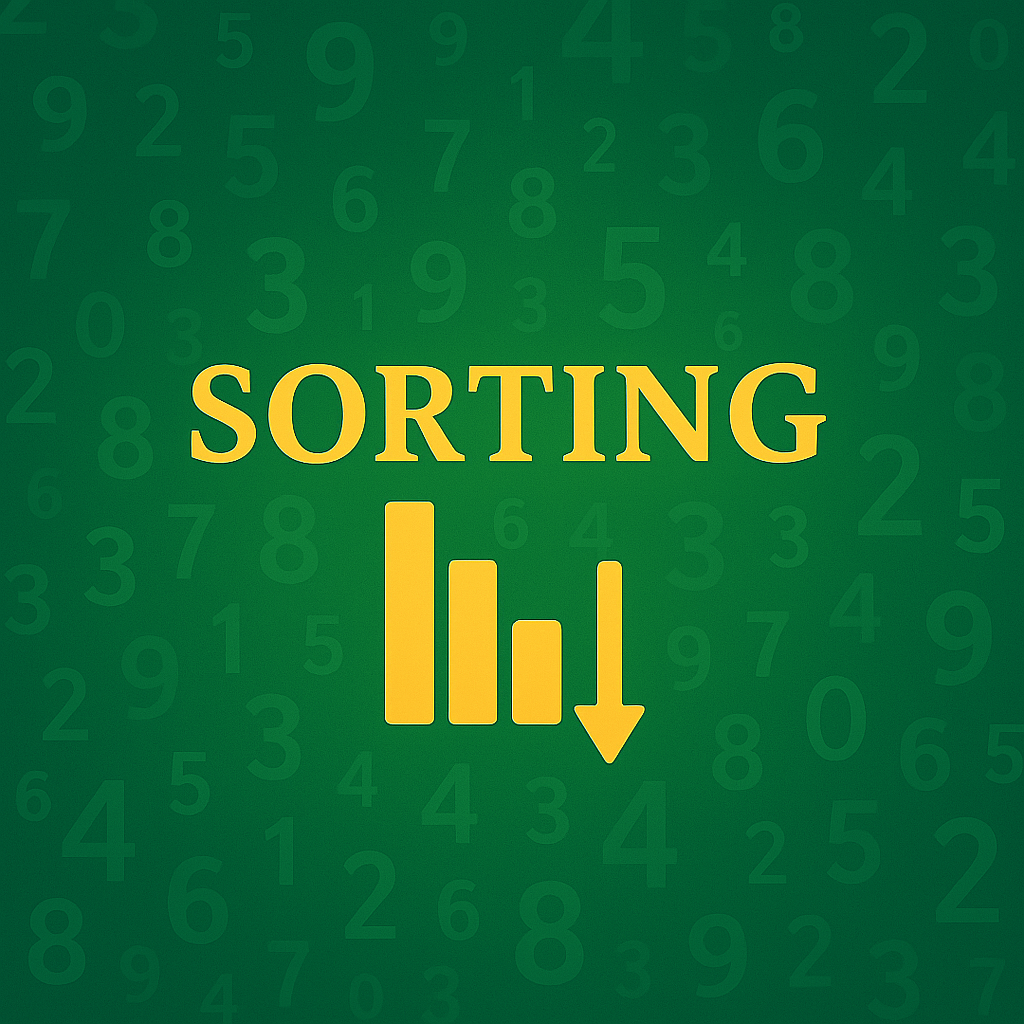
\includegraphics[height=13.88cm, width=17cm, keepaspectratio]{Pics/sort.png}
\end{center}

\chapter{Essential Sorting Techniques }
\phantomsection                      % <-- creates a hyperlink anchor
\label{sec:sorting}
\begin{itemize}
    \item \textbf{Core Sorting Properties:}
    \begin{itemize}
        \item Stability: Preserves order of equal elements (Crucial for multi-key sorts)
        \item Adaptivity: Performs better on partially sorted data (Insertion sort)
        \item In-place: $O(1)$ extra space (Quicksort, Heapsort)
        \item Comparison vs Non-comparison: 
        \begin{itemize}
            \item Comparison: $\Omega(n \log n)$ lower bound
            \item Non-comparison: $O(n)$ possible (Counting, Radix)
        \end{itemize}
    \end{itemize}
    
    \item \textbf{Algorithm Selection Guide:}
    \begin{itemize}
        \item Small arrays ($n \leq 50$): Insertion sort
        \item General purpose: Quicksort (average $O(n \log n)$), Mergesort (stable $O(n \log n)$)
        \item External sorting: Mergesort (disk-friendly)
        \item Integer sorting: 
        \begin{itemize}
            \item Limited range: Counting sort ($O(n + k)$)
            \item Large range: Radix sort ($O(d(n + b))$)
        \end{itemize}
        \item In-place required: Heapsort ($O(1)$ space)
    \end{itemize}
    
    \item \textbf{Custom Comparator Techniques:}
    \begin{itemize}
        \item Multi-key sorting:
        \begin{itemize}
            \item Primary, secondary keys: \texttt{return (a.p == b.p) ? a.q < b.q : a.p < b.p}
        \end{itemize}
        \item Reverse sorting: \texttt{return a > b} (descending)
        \item Absolute value sort: \texttt{return abs(a) < abs(b)}
        \item Custom objects: Define \texttt{operator<} or comparator function
    \end{itemize}
    
    \item \textbf{Advanced Sorting Patterns:}
    \begin{itemize}
        \item Inversion counting:
        \begin{itemize}
            \item Modified mergesort: Count during merge
            \item Applications: Similarity analysis, array disorder measure
        \end{itemize}
        \item K-sorted arrays:
        \begin{itemize}
            \item Heap sort: Min-heap of size $k+1$ ($O(n \log k)$)
            \item Insertion sort: $O(nk)$ for small $k$
        \end{itemize}
        \item Partial sorting:
        \begin{itemize}
            \item Quickselect: $O(n)$ for kth smallest
            \item Partial heapsort: Build heap of size k ($O(n + k \log n)$)
        \end{itemize}
    \end{itemize}
    
    \item \textbf{Counting Sort Optimization:}
    \begin{itemize}
        \item Negative numbers: Shift range to non-negative
        \item Prefix sum array: Calculate output positions
        \item Stability: Process input right-to-left
        \item Character sorting: ASCII values as indices
    \end{itemize}
    
    \item \textbf{Radix Sort Techniques:}
    \begin{itemize}
        \item LSD (Least Significant Digit):
        \begin{itemize}
            \item Fixed-length keys: Numbers, fixed-width strings
            \item Stable sort per digit (usually counting sort)
        \end{itemize}
        \item MSD (Most Significant Digit):
        \begin{itemize}
            \item Variable-length keys: Strings, integers
            \item Recursive bucket sort
        \end{itemize}
        \item Base selection: Power-of-two bases for bitwise optimization
    \end{itemize}
    
    \item \textbf{Hybrid Sorting Approaches:}
    \begin{itemize}
        \item Introsort:
        \begin{itemize}
            \item Quicksort + Heapsort fallback + Insertion sort small arrays
            \item Prevents $O(n^2)$ worst-case
        \end{itemize}
        \item Timsort:
        \begin{itemize}
            \item Mergesort + Insertion sort + Run detection
            \item Python, Java default sort
        \end{itemize}
        \item Bucket sort + Sub-sort:
        \begin{itemize}
            \item Uniformly distributed data
            \item Sort buckets with appropriate algorithm
        \end{itemize}
    \end{itemize}
    
    \item \textbf{Sorting Applications:}
    \begin{itemize}
        \item Two-pointer techniques:
        \begin{itemize}
            \item Two-sum: Sort + left/right pointers
            \item Remove duplicates: Sort + adjacent check
        \end{itemize}
        \item Greedy algorithms:
        \begin{itemize}
            \item Interval scheduling: Sort by finish time
            \item Fractional knapsack: Sort by value/weight ratio
        \end{itemize}
        \item Efficient searching:
        \begin{itemize}
            \item Binary search precondition
            \item Range queries: Sort + binary search
        \end{itemize}
    \end{itemize}
    
    \item \textbf{Edge Cases \& Pitfalls:}
    \begin{itemize}
        \item Empty arrays: Always check size
        \item Single-element arrays: Trivial sort
        \item Duplicate elements: Stability matters
        \item Already sorted/reverse sorted: Test adaptive sorts
        \item Integer overflow: In comparator ($a - b$ fails for large values)
        \item Floating point: Special NaN handling
    \end{itemize}
    
    \item \textbf{Optimization Strategies:}
    \begin{itemize}
        \item Precomputation:
        \begin{itemize}
            \item Compute keys before sorting
            \item Schwartzian transform: Decorate-sort-undecorate
        \end{itemize}
        \item Lazy sorting:
        \begin{itemize}
            \item Partial sorts when possible
            \item Heap-based selection
        \end{itemize}
        \item Parallelization:
        \begin{itemize}
            \item Merge sort: Parallel merges
            \item Quick sort: Parallel partitions
        \end{itemize}
    \end{itemize}
    
    \item \textbf{Common Problem Patterns:}
    \begin{itemize}
        \item Largest number formed: Custom string comparator \texttt{(a+b) > (b+a)}
        \item Meeting rooms: Sort intervals by start time
        \item H-index: Sort citations + find $h$ where $h$ papers have $\geq h$ citations
        \item Merge intervals: Sort by start + merge adjacent
        \item Minimum absolute difference: Sort + adjacent difference
    \end{itemize}
    
    \item \textbf{Language-Specific Nuances:}
    \begin{itemize}
        \item C++:
        \begin{itemize}
            \item \texttt{std::sort}: Introsort, unstable for primitives
            \item \texttt{std::stable\_sort}: Mergesort variant
        \end{itemize}
        \item Java:
        \begin{itemize}
            \item \texttt{Arrays.sort}: Timsort (objects), Dual-Pivot Quicksort (primitives)
            \item Beware: Primitive sort unstable, object sort stable
        \end{itemize}
        \item Python:
        \begin{itemize}
            \item \texttt{list.sort()} and \texttt{sorted()}: Timsort, stable
            \item Key functions: \texttt{key=lambda x: (x[0], -x[1])}
        \end{itemize}
    \end{itemize}
    
    \item \textbf{Debugging \& Testing:}
    \begin{itemize}
        \item Verify stability with duplicate keys
        \item Test with reverse-sorted input
        \item Check corner cases: min/max values, all equal
        \item Validate custom comparators:
        \begin{itemize}
            \item Anti-symmetry: $\text{comp}(a,b) \implies !\text{comp}(b,a)$
            \item Transitivity: $\text{comp}(a,b) \land \text{comp}(b,c) \implies \text{comp}(a,c)$
        \end{itemize}
    \end{itemize}
    
    \item \textbf{Non-comparison Sort Limitations:}
    \begin{itemize}
        \item Counting sort: Integer keys in limited range
        \item Radix sort: Fixed-length keys or strings
        \item Bucket sort: Uniform distribution required
        \item Not applicable for arbitrary comparison functions
    \end{itemize}
\end{itemize}
\section{Sorting-Based DSA Problems Summary Table}
\begin{longtable}{|>{\raggedright\arraybackslash}p{3.2cm}|>{\columncolor{c2}\centering\arraybackslash}p{2.5cm}|>{\columncolor{c3}\raggedright\arraybackslash}p{4.3cm}|>{\columncolor{c4}\raggedright\arraybackslash}p{3.5cm}|>{\columncolor{c5}\color{white}\raggedright\arraybackslash}p{3.5cm}|}
\hline
\rowcolor{rclr}
\textbf{Problem Name} & \textbf{Time Complexity} & \textbf{Idea to Solve} & \textbf{Optimization Tip} & \textbf{Edge Cases} \\
\hline
\endfirsthead
\hline
\textbf{Problem Name} & \textbf{Time Complexity} & \textbf{Idea to Solve} & \textbf{Optimization Tip} & \textbf{Edge Cases} \\
\hline
\endhead
Insertion Sort & $\mathcal{O}(n^2)$ & Insert elements into sorted part by shifting. & Adaptive for nearly sorted arrays. & All elements same, reverse sorted \\
\hline
Bubble Sort & $\mathcal{O}(n^2)$ & Repeatedly swap adjacent elements if out of order. & Use flag to detect sorted pass. & Already sorted array \\
\hline
Selection Sort & $\mathcal{O}(n^2)$ & Select min element and place at front. & Simple, not adaptive or stable. & All elements same \\
\hline
Merge Function (Merge Sort) & $\mathcal{O}(n)$ & Merge two sorted arrays using two pointers. & Extra array needed for merging. & Arrays of unequal sizes \\
\hline
Merge Sort & $\mathcal{O}(n \log n)$ & Divide and recursively merge sorted halves. & Stable sort, good for linked lists. & Already sorted array \\
\hline
Count Inversions in Array & $\mathcal{O}(n \log n)$ & Modified merge sort counting during merge. & Count inversions while merging. & All elements equal, reverse sorted \\
\hline
Partitioning of Array (Lomuto/Hoare) & $\mathcal{O}(n)$ & Rearrange elements around pivot. & Lomuto simpler, Hoare more efficient. & All elements same, pivot at extremes \\
\hline
Quick Sort & Avg: $\mathcal{O}(n \log n)$, Worst: $\mathcal{O}(n^2)$ & Partition and recursively sort sides. & Use random pivot to avoid worst case. & Already sorted or all same elements \\
\hline
Cycle Sort & $\mathcal{O}(n^2)$ & Place elements at correct index by cyclic swaps. & Minimum number of writes. & Duplicates need special care \\
\hline
Heap Sort & $\mathcal{O}(n \log n)$ & Build max-heap, extract max repeatedly. & In-place, not stable. & All elements equal \\
\hline
Counting Sort & $\mathcal{O}(n + k)$ & Count occurrences and compute prefix sum. & Only for small range of integers. & Large value range breaks efficiency \\
\hline
Radix Sort & $\mathcal{O}(n \cdot d)$ & Sort digits using stable sort (e.g., counting). & Works best when digits are bounded. & Very large digits/strings \\
\hline
Bucket Sort & $\mathcal{O}(n + k)$ & Distribute into buckets, then sort each. & Ideal when input is uniformly distributed. & All elements in one bucket \\
\hline
Kth Smallest Element in Array & $\mathcal{O}(n)$ avg & Use Quickselect (partition logic). & Random pivot gives linear avg. & k = 1 or n, duplicates \\
\hline
Chocolate Distribution (Min Diff) & $\mathcal{O}(n \log n)$ & Sort and find min diff of subarrays of size m. & Only sort once and slide window. & m $>$ n, all equal elements \\
\hline
Sort 3 Types of Elements & $\mathcal{O}(n)$ & Dutch National Flag algorithm: 3 pointers. & Single pass with constant space. & All same elements \\
\hline
Merge Overlapping Intervals & $\mathcal{O}(n \log n)$ & Sort by start time, merge if overlap. & Use list/stack to store merged. & Fully nested or same intervals \\
\hline
Meeting Maximum Guests & $\mathcal{O}(n \log n)$ & Sort arrivals and departures, use two pointers. & Keep track of current guests with max. & Overlapping times, same time arrival/departure \\
\hline
\end{longtable}
\clearpage
\newgeometry{margin=1in}
% \documentclass[a4paper,10pt]{article}
% \usepackage[utf8]{inputenc}
% \usepackage{geometry}
% \usepackage[table]{xcolor}
% \usepackage{colortbl}
% \usepackage{color,soul}
% \geometry{margin=0.8in}
% \usepackage{xcolor}
% \usepackage{tikz}
% \usepackage{minted}
% \definecolor{bgcolor}{rgb}{0.8, 0.9, 0.5} % 
% \definecolor{bgcolor1}{rgb}{0.95, 0.95, 0.95} % Light Gray
% \definecolor{bgcolor2}{rgb}{0.85, 0.92, 1.0}  % Soft Blue
% \definecolor{bgcolor3}{rgb}{0.9, 0.85, 1.0}   % Light Purple
% \definecolor{bgcolor4}{rgb}{0.95, 0.88, 0.76} % Warm Beige
% \definecolor{bgcolor5}{rgb}{0.8, 0.95, 0.8}   % Gentle Green
% \definecolor{bgcolor6}{rgb}{1.0, 0.87, 0.87}  % Pastel Red
% \definecolor{bgcolor7}{rgb}{0.86, 0.93, 0.83} % Mint Green
% \definecolor{bgcolor8}{rgb}{0.98, 0.85, 0.94} % Soft Pink
% \definecolor{bgcolor9}{rgb}{0.87, 0.94, 0.98} % Sky Blue
% \definecolor{bgcolor10}{rgb}{0.96, 0.96, 0.82} % Pale Yellow
% 
% % Define a custom background colo
% \begin{document}
\section*{Sorting Problem Solutions}
\noindent\textbf{Problem: Insertion Sort}
\begin{minted}[bgcolor=bgcolor1,frame=lines,framesep=5mm,rulecolor=\color{black},linenos,numbersep=5pt,fontsize=\normalsize]{python}
def insertion_sort(arr):
    """
    In-place insertion sort.
    Time Complexity: O(n^2)
    """
    for i in range(1, len(arr)):
        key = arr[i]
        j = i - 1
        while j >= 0 and arr[j] > key:
            arr[j+1] = arr[j]
            j -= 1
        arr[j+1] = key
\end{minted}

\noindent\textbf{Problem: Bubble Sort}
\begin{minted}[bgcolor=bgcolor2,frame=lines,framesep=5mm,rulecolor=\color{black},linenos,numbersep=5pt,fontsize=\normalsize]{python}
def bubble_sort(arr):
    """
    In-place bubble sort with early exit.
    Time Complexity: O(n^2)
    """
    n = len(arr)
    for i in range(n):
        swapped = False
        for j in range(0, n-1-i):
            if arr[j] > arr[j+1]:
                arr[j], arr[j+1] = arr[j+1], arr[j]
                swapped = True
        if not swapped:
            break
\end{minted}

\noindent\textbf{Problem: Selection Sort}
\begin{minted}[bgcolor=bgcolor3,frame=lines,framesep=5mm,rulecolor=\color{black},linenos,numbersep=5pt,fontsize=\normalsize]{python}
def selection_sort(arr):
    """
    In-place selection sort.
    Time Complexity: O(n^2)
    """
    n = len(arr)
    for i in range(n):
        min_idx = i
        for j in range(i+1, n):
            if arr[j] < arr[min_idx]:
                min_idx = j
        arr[i], arr[min_idx] = arr[min_idx], arr[i]
\end{minted}

\noindent\textbf{Problem: Merge Function (Merge Sort)}
\begin{minted}[bgcolor=bgcolor4,frame=lines,framesep=5mm,rulecolor=\color{black},linenos,numbersep=5pt,fontsize=\normalsize]{python}
def merge(left, right):
    """
    Merge two sorted lists.
    Time Complexity: O(n)
    """
    i = j = 0
    merged = []
    while i < len(left) and j < len(right):
        if left[i] <= right[j]:
            merged.append(left[i]); i += 1
        else:
            merged.append(right[j]); j += 1
    merged.extend(left[i:] or right[j:])
    return merged
\end{minted}

\noindent\textbf{Problem: Merge Sort}
\begin{minted}[bgcolor=bgcolor5,frame=lines,framesep=5mm,rulecolor=\color{black},linenos,numbersep=5pt,fontsize=\normalsize]{python}
def merge_sort(arr):
    """
    Recursive merge sort.
    Time Complexity: O(n log n)
    """
    if len(arr) <= 1:
        return arr
    mid = len(arr)//2
    left = merge_sort(arr[:mid])
    right = merge_sort(arr[mid:])
    return merge(left, right)
\end{minted}

\noindent\textbf{Problem: Count Inversions in Array}
\begin{minted}[bgcolor=bgcolor6,frame=lines,framesep=5mm,rulecolor=\color{black},linenos,numbersep=5pt,fontsize=\normalsize]{python}
def count_inversions(arr):
    """
    Count inversions using modified merge sort.
    Time Complexity: O(n log n)
    """
    def _count(a):
        if len(a) <= 1:
            return a, 0
        mid = len(a)//2
        left, inv_l = _count(a[:mid])
        right, inv_r = _count(a[mid:])
        merged, inv_m = [], 0
        i=j=0
        while i < len(left) and j < len(right):
            if left[i] <= right[j]:
                merged.append(left[i]); i+=1
            else:
            # right[j] < left[i], so it is “inverted” with
            # EVERY element left[i], left[i+1], …, left[-1]
                merged.append(right[j]); j+=1
                inv_m += len(left)-i
        merged += left[i:]+right[j:]
        return merged, inv_l + inv_r + inv_m
    return _count(arr)[1]
\end{minted}

\noindent\textbf{Problem: Partitioning of Array (Lomuto / Hoare)}
\begin{minted}[bgcolor=bgcolor7,frame=lines,framesep=5mm,rulecolor=\color{black},linenos,numbersep=5pt,fontsize=\normalsize]{python}
def lomuto_partition(arr, low, high):
    """
    Lomuto partition scheme.
    """
    pivot = arr[high]
    i = low
    for j in range(low, high):
        if arr[j] < pivot:
            arr[i], arr[j] = arr[j], arr[i]
            i += 1
    arr[i], arr[high] = arr[high], arr[i]
    return i

def hoare_partition(arr, low, high):
    """
    Hoare partition scheme.
    """
    pivot = arr[(low+high)//2]
    i, j = low-1, high+1
    while True:
        i += 1
        while arr[i] < pivot:
            i += 1
        j -= 1
        while arr[j] > pivot:
            j -= 1
        if i >= j:
            return j
        arr[i], arr[j] = arr[j], arr[i]
\end{minted}

\noindent\textbf{Problem: Quick Sort}
\begin{minted}[bgcolor=bgcolor8,frame=lines,framesep=5mm,rulecolor=\color{black},linenos,numbersep=5pt,fontsize=\normalsize]{python}
def quick_sort(arr, low=0, high=None):
    """
    In-place quick sort (Lomuto).
    Time Complexity: O(n log n) avg
    """
    if high is None:
        high = len(arr)-1
    if low < high:
        p = lomuto_partition(arr, low, high)
        quick_sort(arr, low, p-1)
        quick_sort(arr, p+1, high)
\end{minted}

\noindent\textbf{Problem: Cycle Sort}
Why it Guarantees Sorted ?  Cycle sort decomposes the permutation of your array into disjoint cycles, then rotates each cycle into place. Every element is guaranteed to land in its unique “rank” index. Once each cycle is done, no further swaps can disturb the sorted prefix. That establishes correctness.
\begin{minted}[bgcolor=bgcolor9,frame=lines,framesep=5mm,rulecolor=\color{black},linenos,numbersep=5pt,fontsize=\normalsize]{python}
def cycle_sort(arr):
    """
    In-place cycle sort, minimizes the number of writes.
    Time Complexity: O(n^2)
    Returns the total number of writes performed.
    """
    writes = 0
    n = len(arr)

    # We will go through each index as the start of a cycle
    for cycle_start in range(n - 1):
        # The item we want to place into its correct position
        item = arr[cycle_start]
        pos = cycle_start

        # 1) Find where to put the item by counting
        #    how many elements smaller than it exist to its right
        for i in range(cycle_start + 1, n):
            if arr[i] < item:
                pos += 1

        # If the item is already in the correct position, move on
        if pos == cycle_start:
            continue

        # 2) Skip over duplicates to find a free slot
        while arr[pos] == item:
            pos += 1

        # 3) Put the item there (this is a write)
        arr[pos], item = item, arr[pos]
        writes += 1

        # 4) Now rotate the rest of the cycle
        #    until we come back to the starting slot
        while pos != cycle_start:
            pos = cycle_start
            # Find the correct position for the new item
            for i in range(cycle_start + 1, n):
                if arr[i] < item:
                    pos += 1
            # Skip duplicates again
            while arr[pos] == item:
                pos += 1
            # Swap and count the write
            arr[pos], item = item, arr[pos]
            writes += 1

    return writes
\end{minted}

\noindent\textbf{Problem: Heap Sort}
\begin{minted}[bgcolor=bgcolor10,frame=lines,framesep=5mm,rulecolor=\color{black},linenos,numbersep=5pt,fontsize=\normalsize]{python}
def heapify(arr, n, i):
    largest = i
    l, r = 2*i+1, 2*i+2
    if l < n and arr[l] > arr[largest]:
        largest = l
    if r < n and arr[r] > arr[largest]:
        largest = r
    if largest != i:
        arr[i], arr[largest] = arr[largest], arr[i]
        heapify(arr, n, largest)

def heap_sort(arr):
    """
    In-place heap sort.
    Time Complexity: O(n log n)
    """
    n = len(arr)
    for i in range(n//2-1, -1, -1):
        heapify(arr, n, i)
    for i in range(n-1, 0, -1):
        arr[0], arr[i] = arr[i], arr[0]
        heapify(arr, i, 0)
\end{minted}

\noindent\textbf{Problem: Counting Sort}
\begin{minted}[bgcolor=bgcolor1,frame=lines,framesep=5mm,rulecolor=\color{black},linenos,numbersep=5pt,fontsize=\normalsize]{python}
def counting_sort(arr, k=None):
    """
    Non-comparison sort for integers 0..k.
    Time Complexity: O(n+k)
    """
    if not arr:
        return []
    if k is None:
        k = max(arr)
    count = [0]*(k+1)
    for x in arr:
        count[x] += 1
    for i in range(1, k+1):
        count[i] += count[i-1]
    output = [0]*len(arr)
    for x in reversed(arr):     # Traversing right to left for stable sorting
        count[x] -= 1
        output[count[x]] = x
    return output
\end{minted}

\noindent\textbf{Problem: Radix Sort}
\begin{minted}[bgcolor=bgcolor2,frame=lines,framesep=5mm,rulecolor=\color{black},linenos,numbersep=5pt,fontsize=\normalsize]{python}
def radix_sort(arr):
    """
    Least significant digit radix sort for non-negative ints.
    Time Complexity: O(d*(n+ b))
    """
    if not arr:
        return []
    max_val = max(arr)
    exp = 1
    while exp <= max_val:
        buckets = [[] for _ in range(10)]
        for x in arr:
            buckets[(x//exp) % 10].append(x)
        arr = [y for bucket in buckets for y in bucket]
        exp *= 10
    return arr
\end{minted}

\noindent\textbf{Problem: Bucket Sort}
\begin{minted}[bgcolor=bgcolor3,frame=lines,framesep=5mm,rulecolor=\color{black},linenos,numbersep=5pt,fontsize=\normalsize]{python}
def bucket_sort(arr, bucket_size=5):
    """
    Bucket sort for uniformly distributed values.
    Time Complexity: O(n + k log k)
    """
    if not arr:
        return []
    min_val, max_val = min(arr), max(arr)
    bucket_count = (max_val - min_val)//bucket_size + 1
    buckets = [[] for _ in range(bucket_count)]
    for x in arr:
        buckets[(x - min_val)//bucket_size].append(x)
    arr = []
    for b in buckets:
        arr.extend(sorted(b))
    return arr
\end{minted}

\noindent\textbf{Problem: Kth Smallest Element in Array}
\begin{minted}[bgcolor=bgcolor4,frame=lines,framesep=5mm,rulecolor=\color{black},linenos,numbersep=5pt,fontsize=\normalsize]{python}
import random
def kth_smallest(arr, k):
    """
    Quickselect for k-th smallest (1-based).
    Time Complexity: O(n) avg
    """
    def select(lo, hi, k):
        if lo == hi:
            return arr[lo]
        pivot = arr[random.randint(lo, hi)]
        lows = [x for x in arr[lo:hi+1] if x < pivot]
        highs = [x for x in arr[lo:hi+1] if x > pivot]
        mids  = [x for x in arr[lo:hi+1] if x == pivot]
        if k <= len(lows):
            return select(lo, lo+len(lows)-1, k)
        elif k > len(lows) + len(mids):
            return select(lo+len(lows)+len(mids), hi, k-len(lows)-len(mids))
        else:
            return pivot
    return select(0, len(arr)-1, k)
\end{minted}

\noindent\textbf{Problem: Chocolate Distribution (Min Diff)}
\begin{minted}[bgcolor=bgcolor5,frame=lines,framesep=5mm,rulecolor=\color{black},linenos,numbersep=5pt,fontsize=\normalsize]{python}
def min_diff_chocolate(packets, m):
    """
    Find min diff between max and min of any m packets.
    Time Complexity: O(n log n)
    """
    if m == 0 or len(packets) < m:
        return 0
    packets.sort()
    return min(packets[i+m-1] - packets[i] for i in range(len(packets)-m+1))
\end{minted}

\noindent\textbf{Problem: Sort 3 Types of Elements (Dutch National Flag)}
\begin{minted}[bgcolor=bgcolor6,frame=lines,framesep=5mm,rulecolor=\color{black},linenos,numbersep=5pt,fontsize=\normalsize]{python}
def dutch_national_flag(arr):
    """
    Sort array of 0s,1s,2s in one pass.
    Time Complexity: O(n)
    """
    low = mid = 0
    high = len(arr)-1
    while mid <= high:
        if arr[mid] == 0:
            arr[low], arr[mid] = arr[mid], arr[low]
            low += 1; mid += 1
        elif arr[mid] == 1:
            mid += 1
        else:
            arr[mid], arr[high] = arr[high], arr[mid]
            high -= 1
\end{minted}

\noindent\textbf{Problem: Merge Overlapping Intervals}
\begin{minted}[bgcolor=bgcolor7,frame=lines,framesep=5mm,rulecolor=\color{black},linenos,numbersep=5pt,fontsize=\normalsize]{python}
def merge_intervals(intervals):
    """
    Merge all overlapping intervals.
    Time Complexity: O(n log n)
    """
    if not intervals:
        return []
    intervals.sort(key=lambda x: x[0])
    merged = [intervals[0]]
    for start, end in intervals[1:]:
        last_end = merged[-1][1]
        if start <= last_end:
            merged[-1][1] = max(last_end, end)
        else:
            merged.append([start, end])
    return merged
\end{minted}

\noindent\textbf{Problem: Meeting Maximum Guests}
\begin{minted}[bgcolor=bgcolor8,frame=lines,framesep=5mm,rulecolor=\color{black},linenos,numbersep=5pt,fontsize=\normalsize]{python}
def max_guests(arrivals: List[int], departures: List[int]) -> int:
    """
    Finds the maximum number of guests present at the same time
    given lists of arrival and departure times.
    Time Complexity: O(n log n)
    """
    # 1) Build an “events” list: +1 for each arrival, -1 for each departure
    events: List[Tuple[int,int]] = []
    for t in arrivals:
        events.append((t, 1))    # when a guest arrives at t, delta = +1
    for t in departures:
        events.append((t, -1))   # when a guest leaves at t, delta = -1

    # 2) Sort by time; if two events share the same time,
    #    process arrivals (+1) before departures (–1) so we count correctly
    events.sort(key=lambda x: (x[0], -x[1]))

    curr = 0   # current number of guests at the sweep line
    maxg = 0   # record of the maximum seen

    # 3) Sweep through sorted events, updating the count
    for time, delta in events:
        curr += delta            # add or remove a guest
        maxg = max(maxg, curr)   # update peak if needed

    return maxg
\end{minted}
% \end{document}

\newgeometry{margin=0.2in}
\vspace*{47mm}

\begin{center}

{\fontsize{55}{20}\selectfont \textcolor{headingcolor}{\bfseries HASHING}}
\end{center}

\vspace{50mm}

\begin{center}

\includegraphics[height=13.88cm, width=17cm, keepaspectratio]{Pics/hashing.png}
\end{center}

\chapter{Essential Hashing Techniques }
\phantomsection                      % <-- creates a hyperlink anchor
\label{sec:hashing}
\begin{itemize}
    \item \textbf{Hash Function Fundamentals:}
    \begin{itemize}
        \item Integer hashing:
        \begin{itemize}
            \item Identity: $h(x) = x$ (for small bounded integers)
            \item Modulo: $h(x) = x \mod M$ (choose prime $M >$ max elements)
        \end{itemize}
        \item String hashing:
        \begin{itemize}
            \item Polynomial rolling hash: $H(s) = \sum_{i=0}^{n-1} s[i] \cdot p^i \mod M$
            \item Double hashing: Use two different $(p, M)$ pairs for collision safety
            \item Base selection: $p > $ alphabet size, typically 31, 53, or 131
        \end{itemize}
        \item Tuple hashing:
        \begin{itemize}
            \item Combine individual hashes: $h(a,b) = h(a) \oplus (h(b) \ll 1)$ 
            \item Boost method: $hash\_combine(seed, value)$ with bit mixing
        \end{itemize}
    \end{itemize}
    
    \item \textbf{Collision Handling Strategies:}
    \begin{itemize}
        \item Separate chaining: Buckets with linked lists
        \item Open addressing:
        \begin{itemize}
            \item Linear probing: $h(x) + i \mod M$
            \item Quadratic probing: $h(x) + c_1 i + c_2 i^2 \mod M$
            \item Double hashing: $h_1(x) + i \cdot h_2(x) \mod M$
        \end{itemize}
        \item Load factor management: Rehash when $\alpha > 0.7$
    \end{itemize}
    
    \item \textbf{Common Hash-Based Data Structures:}
    \begin{itemize}
        \item Frequency counter: 
        \begin{itemize}
            \item Detect duplicates/anagrams: \texttt{unordered\_map<char, int>}
            \item Sliding window character counts
        \end{itemize}
        \item HashSet operations:
        \begin{itemize}
            \item $O(1)$ membership tests
            \item Union/intersection/difference operations
        \end{itemize}
        \item Prefix hash map:
        \begin{itemize}
            \item Subarray sum equals K: Store cumulative sums
            \item Two-sum variants: Store complements
        \end{itemize}
    \end{itemize}
    
    \item \textbf{Advanced Hashing Patterns:}
    \begin{itemize}
        \item Rabin-Karp string search:
        \begin{itemize}
            \item Rolling hash for substring matching $O(n)$
            \item Update: $H_{new} = (H_{old} - s[i] \cdot p^{L-1}) \cdot p + s[i+L]$
        \end{itemize}
        \item Count-Min Sketch:
        \begin{itemize}
            \item Frequency estimation in streams with multiple hash functions
        \end{itemize}
        \item Bloom filters:
        \begin{itemize}
            \item Space-efficient probabilistic membership test
            \item False positives possible, no false negatives
        \end{itemize}
    \end{itemize}
    
    \item \textbf{Key Optimization Techniques:}
    \begin{itemize}
        \item Precomputation:
        \begin{itemize}
            \item Precompute powers for rolling hash $O(n)$
            \item Precompute prefix hashes for strings
        \end{itemize}
        \item Custom hash functions:
        \begin{itemize}
            \item For user-defined types in C++: specialize \texttt{std::hash}
            \item Avoid systematic collisions with random seeds
        \end{itemize}
        \item Lazy deletion: Mark deleted slots instead of rehashing
    \end{itemize}
    
    \item \textbf{Multi-dimensional Hashing:}
    \begin{itemize}
        \item Grid hashing:
        \begin{itemize}
            \item $H(G) = \sum_{i,j} G[i][j] \cdot p_1^i \cdot p_2^j \mod M$
            \item Subgrid detection with 2D prefix hashes
        \end{itemize}
    \end{itemize}
    
    \item \textbf{Edge Cases \& Pitfalls:}
    \begin{itemize}
        \item Integer overflow: Use modulo arithmetic consistently
        \item Negative modulo: $(x \mod M + M) \mod M$
        \item Empty collections: Hash of empty set should be non-zero
        \item Floating point keys: Avoid direct hashing of floats
        \item Mutable keys: Changing keys after insertion corrupts structure
    \end{itemize}
    
    \item \textbf{Common Problem Patterns:}
    \begin{itemize}
        \item Anagram groups: Sort string or use frequency hash
        \item Subarray sum equals K: Prefix sum + hashmap
        \item Duplicate detection: HashSet for $O(1)$ lookups
        \item Longest substring without repeating chars: Sliding window + char map
        \item Two-sum variants: Store seen elements
        \item Palindrome pairs: Store reverse string hashes
    \end{itemize}
    
    \item \textbf{Hybrid Techniques:}
    \begin{itemize}
        \item Hashing + sliding window: 
        \begin{itemize}
            \item Count distinct substrings with fixed length
            \item Maintain window hash while sliding
        \end{itemize}
        \item Hashing + binary search:
        \begin{itemize}
            \item Longest common substring: Binary search length + hash check
        \end{itemize}
        \item Hashing + DFS/BFS:
        \begin{itemize}
            \item Cycle detection in graphs: Store visited states
            \item Game state memoization
        \end{itemize}
    \end{itemize}
    
    \item \textbf{Complexity Analysis:}
    \begin{itemize}
        \item Average case: $O(1)$ insert/lookup/delete
        \item Worst case: $O(n)$ per operation (all collisions)
        \item Rolling hash: $O(n)$ precomputation, $O(1)$ substring hash
    \end{itemize}
    
    \item \textbf{Language-Specific Tips:}
    \begin{itemize}
        \item C++: 
        \begin{itemize}
            \item \texttt{unordered\_map} vs \texttt{map} (hash vs BST)
            \item Custom hash for user-defined types
        \end{itemize}
        \item Java:
        \begin{itemize}
            \item Override \texttt{hashCode()} and \texttt{equals()} together
            \item \texttt{HashMap} load factor and initial capacity tuning
        \end{itemize}
        \item Python:
        \begin{itemize}
            \item Dictionary resizing when $2/3$ full
            \item Keys must be immutable (tuples ok, lists not)
        \end{itemize}
    \end{itemize}
        
    \item \textbf{Testing \& Debugging:}
    \begin{itemize}
        \item Collision testing: Verify distribution with random inputs
        \item Stress testing: Compare against naive implementation
        \item Hash visualization: Check bit distribution patterns
    \end{itemize}
\end{itemize}
\section{Hashing-Based DSA Problems Summary Table}
\begin{longtable}{|>{\raggedright\arraybackslash}p{3.2cm}|>{\columncolor{c2}\centering\arraybackslash}p{2.5cm}|>{\columncolor{c3}\raggedright\arraybackslash}p{4.3cm}|>{\columncolor{c4}\raggedright\arraybackslash}p{3.5cm}|>{\columncolor{c5}\color{white}\raggedright\arraybackslash}p{3.5cm}|}
\hline
\rowcolor{rclr}
\textbf{Problem Name} & \textbf{Time Complexity} & \textbf{Idea to Solve} & \textbf{Optimization Tip} & \textbf{Edge Cases} \\
\hline
\endfirsthead

\hline
\textbf{Problem Name} & \textbf{Time Complexity} & \textbf{Idea to Solve} & \textbf{Optimization Tip} & \textbf{Edge Cases} \\
\hline
\endhead
Count Distinct Elements in Array & $\mathcal{O}(n)$ & Use unordered set or map to store unique elements. & Use unordered set for $\mathcal{O}(1)$ average ops. & All elements same or all distinct \\
\hline
Frequency of Array Elements & $\mathcal{O}(n)$ & Use hash map to store frequency count. & Use unordered map for fast insert/search. & Large range, negative elements \\
\hline
Intersection and Union of Arrays & $\mathcal{O}(n + m)$ & Use set/map for union and intersection logic. & Store smaller array in hash for space. & One array empty, duplicates \\
\hline
Subarray with Sum = 0 & $\mathcal{O}(n)$ & Use prefix sum and hash set to detect repeats. & Insert prefix sums into hash set as you go. & All zeros, single zero element \\
\hline
Subarray with Xor = k & $\mathcal{O}(n)$ & Use prefix xor and hash set to detect repeats. & Insert prefix xors into hash set as you go. & All zeros, single zero element \\
\hline
Longest Subarray with Given Sum $k$ & $\mathcal{O}(n)$ & Store (prefix sum → index) in hash map. & Keep max length on-the-fly. & Negative numbers, no such subarray \\
\hline
Longest Subarray with Equal 0s and 1s & $\mathcal{O}(n)$ & Replace 0 with -1 and apply prefix sum + hash map. & Transform to subarray with sum = 0. & All 1s or all 0s \\
\hline
Longest Common Binary Subarray with Given Sum & $\mathcal{O}(n)$ & Compute prefix sum diff of both arrays, then find longest span with diff = 0. & Reduce to subarray with 0 difference. & Arrays not same length \\
\hline
Longest Consecutive Subsequence & $\mathcal{O}(n)$ & Insert all in set; for each start of seq, count forward. & Only check seq starting at smallest number. & Unsorted input, repeated numbers \\
\hline
Count Distinct Elements in Every Window & $\mathcal{O}(n)$ & Sliding window with frequency map. & Insert/delete in map while sliding. & Window size $>$ n or = 1 \\
\hline
More than n/k Occurrences in Array & $\mathcal{O}(n)$ & Use hashing to count frequency, then filter $>$ n/k. & Use map of size k to maintain only valid candidate frequencies. & Multiple or no elements qualify \\
\hline
\end{longtable}
\clearpage
\newgeometry{margin=1in}
% \documentclass[a4paper,10pt]{article}
% \usepackage[utf8]{inputenc}
% \usepackage{geometry}
% \usepackage[table]{xcolor}
% \usepackage{colortbl}
% \usepackage{color,soul}
% \geometry{margin=0.8in}
% \usepackage{xcolor}
% \usepackage{tikz}
% \usepackage{minted}
% \definecolor{bgcolor}{rgb}{0.8, 0.9, 0.5} % 
% \definecolor{bgcolor1}{rgb}{0.95, 0.95, 0.95} % Light Gray
% \definecolor{bgcolor2}{rgb}{0.85, 0.92, 1.0}  % Soft Blue
% \definecolor{bgcolor3}{rgb}{0.9, 0.85, 1.0}   % Light Purple
% \definecolor{bgcolor4}{rgb}{0.95, 0.88, 0.76} % Warm Beige
% \definecolor{bgcolor5}{rgb}{0.8, 0.95, 0.8}   % Gentle Green
% \definecolor{bgcolor6}{rgb}{1.0, 0.87, 0.87}  % Pastel Red
% \definecolor{bgcolor7}{rgb}{0.86, 0.93, 0.83} % Mint Green
% \definecolor{bgcolor8}{rgb}{0.98, 0.85, 0.94} % Soft Pink
% \definecolor{bgcolor9}{rgb}{0.87, 0.94, 0.98} % Sky Blue
% \definecolor{bgcolor10}{rgb}{0.96, 0.96, 0.82} % Pale Yellow
% 
% % Define a custom background colo
% \begin{document}
\section*{Hashing Problem Solutions}
\noindent\textbf{Problem: Intersection and Union of Arrays}
\begin{minted}[bgcolor=bgcolor3,frame=lines,framesep=5mm,rulecolor=\color{black},linenos,numbersep=5pt,fontsize=\normalsize]{python}
def intersection_union(a, b):
    """
    Return the intersection and union of two arrays.
    Time Complexity: O(n + m)
    """
    sa, sb = set(a), set(b)
    # Intersection: elements common to both
    inter = sa & sb
    # Union: all elements from both
    uni   = sa | sb
    return list(inter), list(uni)
\end{minted}

\noindent\textbf{Problem: Subarray with Sum = 0}
\begin{minted}[bgcolor=bgcolor4,frame=lines,framesep=5mm,rulecolor=\color{black},linenos,numbersep=5pt,fontsize=\normalsize]{python}
def has_zero_sum_subarray(arr):
    """
    Check if any subarray sums to zero.
    Time Complexity: O(n)
    """
    seen = set([0])
    prefix = 0
    for x in arr:
        prefix += x
        # If prefix repeats or is zero, subarray sum = 0 exists
        if prefix in seen:
            return True
        seen.add(prefix)
    return False
\end{minted}

\noindent\textbf{Problem: Subarray with Xor = k}
\begin{minted}[bgcolor=bgcolor5,frame=lines,framesep=5mm,rulecolor=\color{black},linenos,numbersep=5pt,fontsize=\normalsize]{python}
def has_xor_subarray(arr, k):
    """
    Check if any subarray's xor equals k.
    Time Complexity: O(n)
    """
    seen = set([0])
    prefix = 0
    for x in arr:
        prefix ^= x
        # If prefix^k seen before, subarray xor = k exists
        if (prefix ^ k) in seen:
            return True
        seen.add(prefix)
    return False
\end{minted}

\noindent\textbf{Problem: Longest Subarray with Given Sum k}
\begin{minted}[bgcolor=bgcolor6,frame=lines,framesep=5mm,rulecolor=\color{black},linenos,numbersep=5pt,fontsize=\normalsize]{python}
def longest_subarray_sum_k(arr, k):
    """
    Return length of longest subarray summing to k.
    Time Complexity: O(n)
    """
    first_occ = {0: -1}  # prefix_sum -> first index
    prefix = 0
    max_len = 0
    for i, x in enumerate(arr):
        prefix += x
        # Record first occurrence of this prefix
        if prefix not in first_occ:
            first_occ[prefix] = i
        # Check if a subarray summing to k ends here
        if (prefix - k) in first_occ:
            length = i - first_occ[prefix - k]
            max_len = max(max_len, length)
    return max_len
\end{minted}

\noindent\textbf{Problem: Longest Subarray with Equal 0s and 1s}
\begin{minted}[bgcolor=bgcolor7,frame=lines,framesep=5mm,rulecolor=\color{black},linenos,numbersep=5pt,fontsize=\normalsize]{python}
def longest_equal_01(arr):
    """
    Longest subarray with equal number of 0s and 1s.
    Time Complexity: O(n)
    """
    # Replace 0 with -1, then find longest zero-sum subarray
    mapped = [1 if x==1 else -1 for x in arr]
    first_occ = {0: -1}
    prefix = 0
    max_len = 0
    for i, x in enumerate(mapped):
        prefix += x
        if prefix not in first_occ:
            first_occ[prefix] = i
        max_len = max(max_len, i - first_occ[prefix])
    return max_len
\end{minted}

\noindent\textbf{Problem: Longest Common Binary Subarray with Given Sum}
\begin{minted}[bgcolor=bgcolor8,frame=lines,framesep=5mm,rulecolor=\color{black},linenos,numbersep=5pt,fontsize=\normalsize]{python}
from typing import List, Tuple

def longest_common_sum_subarray(a: List[int], b: List[int]) -> Tuple[int, List[int]]:
    """
    Finds the longest span over which the prefix sums of a and b are equal.
    Returns (length, subarray_of_a).
    """
    n = min(len(a), len(b))
    diff_to_idx = {0: -1}    # maps prefix‐sum diff → earliest index
    diff = 0
    best_len = 0
    best_start = 0

    for i in range(n):
        # update running difference
        diff += a[i] - b[i]

        if diff in diff_to_idx:
            # we’ve seen this diff before at index prev
            prev = diff_to_idx[diff]
            curr_len = i - prev
            if curr_len > best_len:
                best_len = curr_len
                best_start = prev + 1
        else:
            # first time seeing this diff
            diff_to_idx[diff] = i

    # slice out the winner from a
    return best_len, a[best_start : best_start + best_len]

\end{minted}

\noindent\textbf{Problem: Longest Consecutive Subsequence}
\begin{minted}[bgcolor=bgcolor9,frame=lines,framesep=5mm,rulecolor=\color{black},linenos,numbersep=5pt,fontsize=\normalsize]{python}
def longest_consecutive(nums):
    """
    Length of the longest run of consecutive integers.
    Time Complexity: O(n)
    """
    num_set = set(nums)
    max_len = 0
    for x in num_set:
        # Only start at the beginning of a sequence
        if x - 1 not in num_set:
            curr = x
            length = 1
            while curr + 1 in num_set:
                curr += 1
                length += 1
            max_len = max(max_len, length)
    return max_len
\end{minted}

\noindent\textbf{Problem: Count Distinct Elements in Every Window}
\begin{minted}[bgcolor=bgcolor10,frame=lines,framesep=5mm,rulecolor=\color{black},linenos,numbersep=5pt,fontsize=\normalsize]{python}
def distinct_in_windows(arr, k):
    """
    Return list of distinct counts for every window of size k.
    Time Complexity: O(n)
    """
    if k > len(arr): return []
    freq = {}
    distinct = []
    # Initialize first window
    for x in arr[:k]:
        freq[x] = freq.get(x, 0) + 1
    distinct.append(len(freq))
    # Slide window
    for i in range(k, len(arr)):
        # Remove outgoing
        out = arr[i-k]
        freq[out] -= 1
        if freq[out] == 0:
            del freq[out]
        # Add incoming
        in_ = arr[i]
        freq[in_] = freq.get(in_, 0) + 1
        distinct.append(len(freq))
    return distinct
\end{minted}

\noindent\textbf{Problem: More than n/k Occurrences in Array}
\begin{minted}[bgcolor=bgcolor5,frame=lines,framesep=5mm,rulecolor=\color{black},linenos,numbersep=5pt,fontsize=\normalsize]{python}
from typing import List, Any

def more_than_n_over_k(arr: List[Any], k: int) -> List[Any]:
    """
    Return all elements in arr that appear more than len(arr)//k times.
    Uses a Boyer–Moore–style majority‐vote generalization with at most k - 1 candidates.
    Time Complexity: O(n), Space Complexity: O(k)
    """
    n = len(arr)
    if k < 2:
        raise ValueError("k must be at least 2")

    # 1) First pass: find up to k-1 potenstial candidates
    #    Maintain a map of candidate -> “vote count”
    candidates = {}  # type: dict[Any, int]
    for x in arr:
        if x in candidates:
            # increment count if x is already a candidate
            candidates[x] += 1
        elif len(candidates) < k - 1:
            # room to add a new candidate
            candidates[x] = 1
        else:
            # no room: decrement every candidate’s count
            # if any count drops to zero, remove it
            to_delete = []
            for c in candidates:
                candidates[c] -= 1
                if candidates[c] == 0:
                    to_delete.append(c)
            for c in to_delete:
                del candidates[c]

    # 2) Second pass: verify actual frequencies of the remaining candidates
    counts = {c: 0 for c in candidates}
    for x in arr:
        if x in counts:
            counts[x] += 1

    # 3) Collect those whose true count exceeds n//k
    result = []
    threshold = n // k
    for c, cnt in counts.items():
        if cnt > threshold:
            result.append(c)

    return result
\end{minted}
% \end{document}

\newgeometry{margin=0.2in}
\vspace*{47mm}

\begin{center}

{\fontsize{55}{20}\selectfont \textcolor{headingcolor}{\bfseries STRING}}
\end{center}

\vspace{50mm}

\begin{center}

\includegraphics[height=13.88cm, width=17cm, keepaspectratio]{Pics/string.png}
\end{center}

\chapter{Essential String Techniques }
\phantomsection                      % <-- creates a hyperlink anchor
\label{sec:string}
\begin{itemize}
    \item \textbf{Character Manipulation Fundamentals:}
    \begin{itemize}
        \item ASCII conversions:
        \begin{itemize}
            \item \texttt{char - '0'} for digit conversion
            \item \texttt{ch \& 31} for case-insensitive bitmask
        \end{itemize}
        \item Character classification:
        \begin{itemize}
            \item \texttt{isdigit(), isalpha(), isalnum()}
            \item Custom bitmask: \texttt{mask |= 1 << (ch - 'a')}
        \end{itemize}
        \item Case conversion:
        \begin{itemize}
            \item \texttt{ch \^{} 32} to toggle case
            \item \texttt{ch | ' '} to lowercase, \texttt{ch \& '\_'} to uppercase
        \end{itemize}
    \end{itemize}
    
    \item \textbf{String Traversal Patterns:}
    \begin{itemize}
        \item Two pointers:
        \begin{itemize}
            \item Opposite-direction: Palindrome checks
            \item Same-direction: Remove duplicates
        \end{itemize}
        \item Sliding window:
        \begin{itemize}
            \item Longest substring without repeating: HashMap + left pointer
            \item Minimum window substring: Frequency map + counter
        \end{itemize}
        \item Reverse traversal:
        \begin{itemize}
            \item Process from end (number addition, path normalization)
            \item Avoid recomputation with suffix arrays
        \end{itemize}
    \end{itemize}
    
    \item \textbf{Substring Search Algorithms:}
    \begin{itemize}
        \item Knuth-Morris-Pratt (KMP):
        \begin{itemize}
            \item Prefix function: \texttt{lps[i] = longest proper prefix/suffix}
            \item Complexity: $O(n + m)$ for text and pattern
        \end{itemize}
        \item Rabin-Karp:
        \begin{itemize}
            \item Rolling hash: $H = (H \cdot \text{base} + \text{ch}) \mod p$
            \item Double hashing for collision safety
        \end{itemize}
        \item Boyer-Moore:
        \begin{itemize}
            \item Bad character rule: Jump tables
            \item Good suffix rule: Complex but efficient in practice
        \end{itemize}
    \end{itemize}
    
    \item \textbf{Palindromic String Techniques:}
    \begin{itemize}
        \item Center expansion:
        \begin{itemize}
            \item Odd/even centers: $O(n^2)$ time, $O(1)$ space
            \item Count palindromic substrings
        \end{itemize}
        \item Manacher's algorithm:
        \begin{itemize}
            \item Linear time: Maintain center and right boundary
            \item Transform: Insert \# between characters
        \end{itemize}
        \item Longest palindromic subsequence:
        \begin{itemize}
            \item Convert to LCS: \texttt{S} vs \texttt{reverse(S)}
            \item Interval DP: \texttt{dp[i][j] = dp[i+1][j-1] + 2} if match
        \end{itemize}
    \end{itemize}
    
    \item \textbf{String Transformation Patterns:}
    \begin{itemize}
        \item Edit distance:
        \begin{itemize}
            \item Wagner-Fischer: \texttt{dp[i][j] = min(insert, delete, replace)}
            \item Space optimization: Two rows
        \end{itemize}
        \item Anagram detection:
        \begin{itemize}
            \item Frequency maps: \texttt{int[26]} for alphabets
            \item Sorting: \texttt{sort(s) == sort(t)}
        \end{itemize}
        \item Group shifted strings:
        \begin{itemize}
            \item Normalize: \texttt{(s[i] - s[0] + 26) \% 26}
            \item Encode as tuple of differences
        \end{itemize}
    \end{itemize}
    
    \item \textbf{String Parsing Techniques:}
    \begin{itemize}
        \item Tokenization:
        \begin{itemize}
            \item State machine: Track in-word/in-space
            \item Library functions: \texttt{split(), strtok()}
        \end{itemize}
        \item Syntax parsing:
        \begin{itemize}
            \item Stack-based: Valid parentheses, tag validation
            \item Recursive descent: Calculator expressions
        \end{itemize}
        \item Path normalization:
        \begin{itemize}
            \item Split by '/', handle '.' and '..' with stack
        \end{itemize}
    \end{itemize}
    
    \item \textbf{Advanced Data Structures:}
    \begin{itemize}
        \item Trie (Prefix tree):
        \begin{itemize}
            \item Structure: \texttt{children[26], isEnd}
            \item Applications: Autocomplete, word search
        \end{itemize}
        \item Suffix array:
        \begin{itemize}
            \item Construct: $O(n \log n)$ with doubling
            \item LCP array: Longest common prefix between suffixes
        \end{itemize}
        \item Suffix automaton:
        \begin{itemize}
            \item Count distinct substrings: $\sum \text{len}(state) - \text{len}(\text{link}(state))$
            \item Find longest repeating substring
        \end{itemize}
    \end{itemize}
    
    \item \textbf{Regular Expression Patterns:}
    \begin{itemize}
        \item Basic matching:
        \begin{itemize}
            \item '.' as wildcard, '*' for repetition
            \item Recursive/DP: Match remaining after '*'
        \end{itemize}
        \item Finite automata:
        \begin{itemize}
            \item NFA: Backtracking implementation
            \item DFA: Table-driven (efficient but large)
        \end{itemize}
    \end{itemize}
    
    \item \textbf{String Compression Techniques:}
    \begin{itemize}
        \item Run-length encoding:
        \begin{itemize}
            \item Encode: \texttt{char + count}
            \item Decode: Expand counts
        \end{itemize}
        \item Huffman coding:
        \begin{itemize}
            \item Min-heap: Merge lowest frequency nodes
            \item Prefix codes: No ambiguity
        \end{itemize}
        \item LZW compression:
        \begin{itemize}
            \item Dictionary-based: Grow codebook
            \item Used in GIF, PDF
        \end{itemize}
    \end{itemize}
    
    \item \textbf{Edge Cases \& Pitfalls:}
    \begin{itemize}
        \item Empty string: Check length before access
        \item Single character strings
        \item Case sensitivity: Often overlooked
        \item Unicode handling: UTF-8 vs ASCII
        \item String immutability: Concatenation $O(n^2)$ time
        \item Null terminators: C-style strings
    \end{itemize}
    
    \item \textbf{Optimization Strategies:}
    \begin{itemize}
        \item Precomputation:
        \begin{itemize}
            \item Prefix sums: For character frequencies
            \item Rolling hash: Precompute powers
        \end{itemize}
        \item Early termination:
        \begin{itemize}
            \item Break when mismatch found
            \item Stop when impossible to improve
        \end{itemize}
        \item Space-time tradeoffs:
        \begin{itemize}
            \item Character maps vs full hash maps
            \item In-place modifications
        \end{itemize}
    \end{itemize}
    
    \item \textbf{Common Problem Patterns:}
    \begin{itemize}
        \item Longest substring without repeating: Sliding window + map
        \item String permutations: Frequency map + two pointers
        \item Minimum window substring: Expand right, contract left
        \item Word break: DP with substring lookup
        \item Encode/decode strings: Delimiters or length prefix
    \end{itemize}
    
    \item \textbf{Hybrid Techniques:}
    \begin{itemize}
        \item KMP + DP: Pattern matching with wildcards
        \item Trie + DFS: Word search in grid
        \item Suffix array + binary search: Longest common substring
        \item Rolling hash + sliding window: Rabin-Karp for multiple patterns
    \end{itemize}
    
    \item \textbf{Language-Specific Nuances:}
    \begin{itemize}
        \item Python:
        \begin{itemize}
            \item Strings immutable: Use list for mutation, \texttt{''.join()}
            \item Slicing: $O(k)$ for slice of length $k$
        \end{itemize}
        \item Java:
        \begin{itemize}
            \item \texttt{StringBuilder} for mutable operations
            \item \texttt{intern()} for constant pool
        \end{itemize}
        \item C++:
        \begin{itemize}
            \item \texttt{std::string::npos} for not found
            \item \texttt{substr(start, length)} $O(n)$ operation
        \end{itemize}
    \end{itemize}
    
    \item \textbf{Testing \& Debugging:}
    \begin{itemize}
        \item Unicode tests: Emojis, multi-byte characters
        \item Empty and single-character inputs
        \item Repeated character strings
        \item Case-sensitive vs insensitive checks
        \item Off-by-one in loops: Use \texttt{<= length} vs \texttt{< length}
    \end{itemize}
    
    \item \textbf{Advanced Applications:}
    \begin{itemize}
        \item Z-algorithm: Linear time pattern search
    \end{itemize}
\end{itemize}
\section{String-Based DSA Problems Summary Table}
\begin{longtable}{|>{\raggedright\arraybackslash}p{3.2cm}|>{\columncolor{c2}\centering\arraybackslash}p{2.5cm}|>{\columncolor{c3}\raggedright\arraybackslash}p{4.3cm}|>{\columncolor{c4}\raggedright\arraybackslash}p{3.5cm}|>{\columncolor{c5}\color{white}\raggedright\arraybackslash}p{3.5cm}|}
\hline
\rowcolor{rclr}
\textbf{Problem Name} & \textbf{Time Complexity} & \textbf{Idea to Solve} & \textbf{Optimization Tip} & \textbf{Edge Cases} \\
\hline
\endfirsthead

\hline
\rowcolor{rclr}
\textbf{Problem Name} & \textbf{Time Complexity} & \textbf{Idea to Solve} & \textbf{Optimization Tip} & \textbf{Edge Cases} \\
\hline
\endhead
Reverse Words in a Given String & $\mathcal{O}(n)$ & Reverse whole string, then reverse each word. & Trim extra spaces and handle in-place if needed. & Multiple spaces, trailing spaces \\
\hline
Is Subsequence of Other & $\mathcal{O}(n)$ & Two pointer approach to match characters. & Return early when end is reached. & Empty subsequence, longer target \\
\hline
Sort Anagrams Together & $O(n \cdot k \log k)$ & Use hashmap of sorted string → list of anagrams & Use tuple(sorted(word)) as key & Empty strings \\
\hline
Naive Pattern Searching & $\mathcal{O}((n - m + 1) \cdot m)$ & Slide pattern over text and check match at each index. & Stop inner loop early on mismatch. & Pattern at end, repeated chars \\
\hline
Rabin-Karp Algorithm & Avg: $\mathcal{O}(n + m)$, Worst: $\mathcal{O}(nm)$ & Use rolling hash to compare hash values of pattern and text. & Use large prime modulus to avoid collisions. & Hash collision, overlapping matches \\
\hline
KMP Algorithm & $\mathcal{O}(n + m)$ & Preprocess LPS array to skip redundant checks. & Use LPS array for efficient jump in pattern. & Pattern equals text, repeated patterns \\
\hline
Check if Strings are Rotations & $\mathcal{O}(n)$ & Concatenate original string with itself and search other. & Use KMP or inbuilt substring search. & Same strings, empty strings \\
\hline
Longest Substring with Distinct Characters & $\mathcal{O}(n)$ & Use sliding window with hash set to track seen characters. & Use two pointers to maintain window. & All characters same, all distinct \\
\hline
Lexicographical Rank of a String & $\mathcal{O}(n^2)$ or $\mathcal{O}(n)$ with precomputation & Count smaller chars on right and use factorial logic. & Precompute factorials and use freq count. & Duplicate characters, repeated pattern \\
\hline
Anagram Search & $\mathcal{O}(n)$ & Sliding window + freq count comparison. (Note: Basic anagram search can't done using xor). & Use count arrays or hash map with difference counter. & Overlapping anagrams, repeated chars \\
\hline
Longest Palindromic Substring & $O(n^2)$ & Expand around center for even and odd palindrome & Expand preferred: less space & Multiple longest substrings \\
\hline

Count of Distinct Substrings 
  & \(O(n^2\log n)\) 
  & Build a suffix array in \(O(n\log n)\), compute the LCP array in \(O(n)\), then use  
    \(\frac{n(n+1)}2 - \sum\mathrm{LCP}\) to count distinct substrings. 
  & \(O(n)\) via suffix‐automaton  
    (or \(O(n\log n)\) with suffix‐array + LCP) 
  & \(n=0\) (empty string),  
    all characters identical 
\\\hline

Longest Repeating Substring 
  & \(O(n^2)\) brute‐force or DP 
  & Construct suffix‐array + LCP; optionally binary‐search on substring length and
    check via LCP (or rolling‐hash) 
  & \(O(n\log n)\) using suffix‐array + binary‐search 
    (or \(O(n)\) with SA + direct LCP scan) 
  & All characters distinct (no repeat),  
    \(n<2\) 
\\\hline
Z-function String Matching & $O(n)$ & $Z[i]$ = length of prefix starting at $i$ matching $s[0..]$ & Useful for pattern matching: use "$P\$T$" trick & Pattern at end or not found \\
\hline
\end{longtable}
\clearpage
\newgeometry{margin=1in}
% \documentclass[a4paper,10pt]{article}
% \usepackage[utf8]{inputenc}
% \usepackage{geometry}
% \usepackage[table]{xcolor}
% \usepackage{colortbl}
% \usepackage{color,soul}
% \geometry{margin=0.8in}
% \usepackage{xcolor}
% \usepackage{tikz}
% \usepackage{minted}
% \definecolor{bgcolor}{rgb}{0.8, 0.9, 0.5} % 
% \definecolor{bgcolor1}{rgb}{0.95, 0.95, 0.95} % Light Gray
% \definecolor{bgcolor2}{rgb}{0.85, 0.92, 1.0}  % Soft Blue
% \definecolor{bgcolor3}{rgb}{0.9, 0.85, 1.0}   % Light Purple
% \definecolor{bgcolor4}{rgb}{0.95, 0.88, 0.76} % Warm Beige
% \definecolor{bgcolor5}{rgb}{0.8, 0.95, 0.8}   % Gentle Green
% \definecolor{bgcolor6}{rgb}{1.0, 0.87, 0.87}  % Pastel Red
% \definecolor{bgcolor7}{rgb}{0.86, 0.93, 0.83} % Mint Green
% \definecolor{bgcolor8}{rgb}{0.98, 0.85, 0.94} % Soft Pink
% \definecolor{bgcolor9}{rgb}{0.87, 0.94, 0.98} % Sky Blue
% \definecolor{bgcolor10}{rgb}{0.96, 0.96, 0.82} % Pale Yellow
% 
% % Define a custom background colo
% \begin{document}
\section*{String Problem Solutions}
\noindent\textbf{Problem: Is Subsequence of Other}
\begin{minted}[
bgcolor=bgcolor5,
frame=lines,
framesep=5mm,
rulecolor=\color{black},
linenos,
numbersep=5pt,
fontsize=\normalsize
]{python}
def is_subsequence(s: str, t: str) -> bool:
    """
    Return True if `s` is a subsequence of `t`, i.e. all characters of s
    appear in order (but not necessarily contiguously) in t.
    """
    i, j = 0, 0
    # i scans s, j scans t
    while i < len(s) and j < len(t):
        if s[i] == t[j]:
            # match: consume s[i]
            i += 1
        # always advance t’s pointer
        j += 1
    # if we’ve consumed all of s, it’s a subsequence
    return i == len(s)
\end{minted}
\noindent\textbf{Problem: Group the Anagrams}
\begin{minted}[
bgcolor=bgcolor6,
frame=lines,
framesep=5mm,
rulecolor=\color{black},
linenos,
numbersep=5pt,
fontsize=\normalsize
]{python}
from collections import defaultdict
from typing import List

def group_anagrams(words: List[str]) -> List[List[str]]:
    """
    Group a list of words into anagrams.
    """
    buckets = defaultdict(list)
    
    for w in words:
        # sort the word’s letters to form the key
        key = tuple(sorted(w))
        buckets[key].append(w)
    
    # return the grouped anagrams
    return list(buckets.values())
\end{minted}
\noindent\textbf{Problem:} Naive Pattern Searching
\begin{minted}[
bgcolor=bgcolor6,
frame=lines,
framesep=5mm,
rulecolor=\color{black},
linenos,
numbersep=5pt,
fontsize=\normalsize
]{python}
def naive_pattern_search(text: str, pat: str) -> List[int]:
    """
    Return start-indices where pat occurs in text by brute force.
    O(n*m) time.
    """
    n, m = len(text), len(pat)
    matches = []
    for i in range(n - m + 1):
        # check match at offset i
        for j in range(m):
            if text[i + j] != pat[j]:
                break
        else:
            matches.append(i)
    return matches
\end{minted}
\noindent\textbf{Problem: Rabin–Karp Algorithm}
\begin{minted}[
bgcolor=bgcolor7,
frame=lines,
framesep=5mm,
rulecolor=\color{black},
linenos,
numbersep=5pt,
fontsize=\normalsize
]{python}
def rabin_karp_search(text: str, pat: str,
                      base: int = 256, mod: int = 101) -> List[int]:
    """
    Find all occurrences of pat in text using rolling‐hash.
    Average O(n+m), worst O(n*m) if many hash collisions.
    """
    n, m = len(text), len(pat)
    if m > n:
        return []

    # precompute high-order base^(m-1) % mod
    h = pow(base, m - 1, mod)
    p_hash = t_hash = 0
    res = []

    # initial hash for pattern & first window
    for i in range(m):
        p_hash = (p_hash * base + ord(pat[i])) % mod
        t_hash = (t_hash * base + ord(text[i])) % mod

    for i in range(n - m + 1):
        # if hashes match, verify actual substring
        if p_hash == t_hash and text[i:i+m] == pat:
            res.append(i)
        # roll the window
        if i < n - m:
            t_hash = (t_hash - ord(text[i]) * h) % mod
            t_hash = (t_hash * base + ord(text[i + m])) % mod
            t_hash = (t_hash + mod) % mod  # ensure positive
    return res
\end{minted}
\noindent\textbf{Problem:} Knuth–Morris–Pratt (KMP) Algorithm
\begin{minted}[
bgcolor=bgcolor3,
frame=lines,
framesep=5mm,
rulecolor=\color{black},
linenos,
numbersep=5pt,
fontsize=\normalsize
]{python}
def kmp_search(text: str, pat: str) -> List[int]:
    """
    Return all start-indices of pat in text using KMP in O(n+m).
    """
    # build lps (longest proper‐prefix‐that‐is‐suffix) table
    m = len(pat)
    lps = [0] * m
    length = 0
    i = 1
    while i < m:
        if pat[i] == pat[length]:
            length += 1
            lps[i] = length
            i += 1
        elif length:
            length = lps[length - 1]
        else:
            lps[i] = 0
            i += 1

    # search
    res = []
    i = j = 0  # i→text, j→pat
    n = len(text)
    while i < n:
        if text[i] == pat[j]:
            i += 1
            j += 1
            if j == m:
                res.append(i - m)
                j = lps[j - 1]
        else:
            if j:
                j = lps[j - 1]
            else:
                i += 1
    return res
\end{minted}
\noindent\textbf{Problem:} Check if Strings are Rotations
\begin{minted}[
bgcolor=bgcolor8,
frame=lines,
framesep=5mm,
rulecolor=\color{black},
linenos,
numbersep=5pt,
fontsize=\normalsize
]{python}
def are_rotations(s1: str, s2: str) -> bool:
    """
    Return True if s2 is a rotation of s1 by checking s2 in s1+s1.
    O(n) time.
    """
    return len(s1) == len(s2) and s2 in (s1 + s1)
\end{minted}
\noindent\textbf{Problem:} Longest Substring with Distinct Characters
\begin{minted}[
bgcolor=bgcolor2,
frame=lines,
framesep=5mm,
rulecolor=\color{black},
linenos,
numbersep=5pt,
fontsize=\normalsize
]{python}
def longest_unique_substring(s: str) -> Tuple[int, str]:
    """
    Return (length, substring) of the longest substring without repeating chars.
    Uses sliding window + hashmap in O(n).
    """
    start = max_len = 0
    max_sub = ""
    last_seen = {}

    for i, c in enumerate(s):
        if c in last_seen and last_seen[c] >= start:
            # move window past previous occurrence
            start = last_seen[c] + 1
        last_seen[c] = i
        curr_len = i - start + 1
        if curr_len > max_len:
            max_len = curr_len
            max_sub = s[start:i+1]

    return max_len, max_sub
\end{minted}
\noindent\textbf{Problem:} Lexicographical rank of a String
\begin{minted}[
bgcolor=bgcolor4,
frame=lines,
framesep=5mm,
rulecolor=\color{black},
linenos,
numbersep=5pt,
fontsize=\normalsize
]{python}

def lexicographic_rank(s: str) -> int:
    """
    Return 1-based rank of s among its permutations (all chars unique).
    O(n^2) due to counting smaller chars for each position.
    """
    n = len(s)
    rank = 1
    for i in range(n):
        # count chars smaller than s[i] to its right
        smaller = sum(1 for j in range(i+1, n) if s[j] < s[i])
        rank += smaller * factorial(n - i - 1)
    return rank
\end{minted}
\noindent\textbf{Problem:} Longest Palindromic Substring
\begin{minted}[
bgcolor=bgcolor1,
frame=lines,
framesep=5mm,
rulecolor=\color{black},
linenos,
numbersep=5pt,
fontsize=\normalsize
]{python}
def longest_palindromic_substring(s: str) -> str:
    """
    Return the longest palindromic substring via expand‐around‐center in O(n^2).
    """
    if not s:
        return ""

    def expand(l: int, r: int) -> Tuple[int,int]:
        # expand as long as s[l]==s[r]
        while l >= 0 and r < len(s) and s[l] == s[r]:
            l -= 1
            r += 1
        return l+1, r-1  # back up one step

    start = end = 0
    for i in range(len(s)):
        # odd-length palindrome
        l1, r1 = expand(i, i)
        # even-length palindrome
        l2, r2 = expand(i, i+1)
        # pick the longer of the two
        if r1 - l1 > end - start:
            start, end = l1, r1
        if r2 - l2 > end - start:
            start, end = l2, r2

    return s[start:end+1]

\end{minted}
\noindent\textbf{Problem:} Z-function String Matching
\begin{minted}[
bgcolor=bgcolor10,
frame=lines,
framesep=5mm,
rulecolor=\color{black},
linenos,
numbersep=5pt,
fontsize=\normalsize
]{python}
def z_function(s: str) -> List[int]:
    """
    Compute the Z-array for s where Z[i] = max length of prefix
    starting at s[i]. Runs in O(len(s)).
    """
    n = len(s)
    Z = [0]*n
    l = r = 0
    for i in range(1, n):
        if i <= r:
            Z[i] = min(r - i + 1, Z[i-l])
        while i + Z[i] < n and s[Z[i]] == s[i + Z[i]]:
            Z[i] += 1
        if i + Z[i] - 1 > r:
            l, r = i, i + Z[i] - 1
    return Z

def z_search(text: str, pat: str) -> List[int]:
    """
    Find all occurrences of pat in text in O(n+m) via Z-function.
    """
    concat = pat + "$" + text
    Z = z_function(concat)
    m = len(pat)
    res = []
    for i in range(m+1, len(concat)):
        if Z[i] == m:
            # match starts at i-(m+1)
            res.append(i - m - 1)
    return res
\end{minted}
\noindent\textbf{Problem:} Anagram Search
\begin{minted}[
bgcolor=bgcolor,
frame=lines,
framesep=5mm,
rulecolor=\color{black},
linenos,
numbersep=5pt,
fontsize=\normalsize
]{python}
def find_anagrams(text: str, pat: str) -> List[int]:
    """
    Return all start-indices where text[i:i+len(pat)] is an anagram of pat.
    Uses sliding window + counters in O(n).
    """
    n, m = len(text), len(pat)
    if m > n:
        return []

    pat_count = Counter(pat)
    win_count = Counter()
    res = []

    for i, c in enumerate(text):
        win_count[c] += 1
        # shrink window when size > m
        if i >= m:
            left_char = text[i-m]
            if win_count[left_char] == 1:
                del win_count[left_char]
            else:
                win_count[left_char] -= 1
        # compare when we have a full-size window
        if i >= m-1 and win_count == pat_count:
            res.append(i - m + 1)

    return res
\end{minted}
% \end{document}

\newgeometry{margin=0.2in}
\vspace*{47mm}

\begin{center}

{\fontsize{55}{20}\selectfont \textcolor{headingcolor}{\bfseries LINKED-LIST}}
\end{center}

\vspace{50mm}

\begin{center}
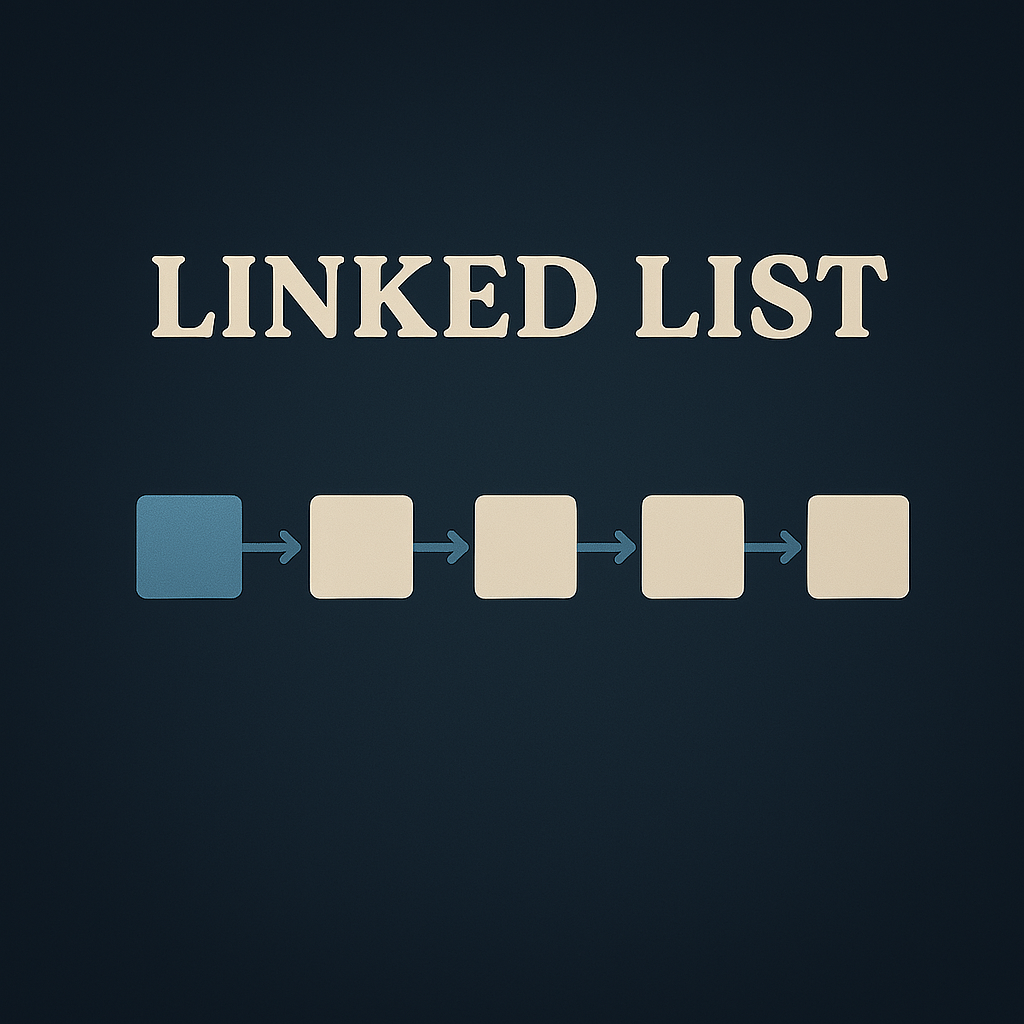
\includegraphics[height=13.88cm, width=17cm, keepaspectratio]{Pics/linkedlist.png}
\end{center}

\chapter{Essential Linked List Techniques }
\phantomsection                      % <-- creates a hyperlink anchor
\label{sec:linked}
\begin{itemize}
    \item \textbf{Pointer Manipulation Fundamentals:}
    \begin{itemize}
        \item Iterative traversal: 
        \begin{itemize}
            \item \texttt{while (current != null) \{ ... current = current.next; \}}
            \item Always check \texttt{current.next} before accessing
        \end{itemize}
        \item Node deletion: 
        \begin{itemize}
            \item Standard: \texttt{prev.next = current.next}
            \item Without prev pointer: Copy \texttt{next} node data and skip
        \end{itemize}
        \item Pointer assignment order: Critical for reversal and insertion
    \end{itemize}
    
    \item \textbf{Two Pointers Technique:}
    \begin{itemize}
        \item Fast-slow pointers:
        \begin{itemize}
            \item Cycle detection: Fast (2x) catches slow if cycle exists
            \item Middle node: Slow at middle when fast reaches end
            \item Cycle length: Freeze slow, move fast until meet again
        \end{itemize}
        \item Distance-based pointers:
        \begin{itemize}
            \item Nth from end: Advance first pointer N steps, then move both
            \item Intersection: Traverse both lists, reset pointers at end
        \end{itemize}
    \end{itemize}
    
    \item \textbf{Recursion Patterns:}
    \begin{itemize}
        \item Reverse linked list:
        \begin{itemize}
            \item Base case: \texttt{if (head == null || head.next == null) return head}
            \item Recurse: \texttt{newHead = reverse(head.next)}
            \item Adjust: \texttt{head.next.next = head; head.next = null}
        \end{itemize}
        \item Tree-like operations:
        \begin{itemize}
            \item Merge two sorted lists: Compare heads and recurse
            \item Validate palindrome: Recurse to middle and compare while backtracking
        \end{itemize}
        \item Stack-based processing:
        \begin{itemize}
            \item Process nodes backwards (reverse order)
            \item Add numbers from least significant digit
        \end{itemize}
    \end{itemize}
    
    \item \textbf{Dummy Node Technique:}
    \begin{itemize}
        \item Usage scenarios:
        \begin{itemize}
            \item Head might change (reversal, partition)
            \item Avoiding null pointer checks
            \item Merging multiple lists
        \end{itemize}
        \item Implementation:
        \begin{itemize}
            \item \texttt{ListNode dummy = new ListNode(0)}
            \item \texttt{dummy.next = head}
            \item Return \texttt{dummy.next}
        \end{itemize}
    \end{itemize}
    
    \item \textbf{Cycle Detection \& Handling:}
    \begin{itemize}
        \item Floyd's algorithm:
        \begin{itemize}
            \item Phase 1: Detect cycle (fast meets slow)
            \item Phase 2: Find start - reset slow to head, advance both 1x speed
        \end{itemize}
        \item Cycle removal: Break link at start node
        \item Cycle length: Measure distance between meeting points
    \end{itemize}
    
    \item \textbf{Advanced Reversal Patterns:}
    \begin{itemize}
        \item Reverse in groups:
        \begin{itemize}
            \item Iterative: Reverse K nodes, connect to next group
            \item Recursive: Reverse first K, recurse for rest
        \end{itemize}
        \item Reverse between indices:
        \begin{itemize}
            \item Mark node before start, reverse segment, reconnect
        \end{itemize}
        \item Reverse alternately: Skip nodes between reversed groups
    \end{itemize}
    
    \item \textbf{Merge Patterns:}
    \begin{itemize}
        \item Merge two sorted lists:
        \begin{itemize}
            \item Iterative: Compare and build new list
            \item Recursive: Smaller node.next = merge(remaining)
        \end{itemize}
        \item Merge K sorted lists:
        \begin{itemize}
            \item Priority queue: O(N log K) time
            \item Divide and conquer: Pairwise merging
        \end{itemize}
        \item Merge sort on linked lists:
        \begin{itemize}
            \item Find middle (fast-slow), recurse halves, merge
        \end{itemize}
    \end{itemize}
    
    \item \textbf{Deep Copy Techniques:}
    \begin{itemize}
        \item Copy with random pointers:
        \begin{itemize}
            \item Two-pass: Create node map, then connect pointers
            \item Weaving: $A->A'->B->B'$, then separate
        \end{itemize}
        \item Clone complex structures: Use hashmap for O(1) node access
    \end{itemize}
    
    \item \textbf{Edge Cases:}
    \begin{itemize}
        \item Empty list (head = null)
        \item Single node list
        \item Two-node list (tests pointer swaps)
        \item Head/tail modification cases
        \item Cyclic lists
        \item Large lists (recursion stack overflow)
    \end{itemize}
    
    \item \textbf{Optimization Strategies:}
    \begin{itemize}
        \item Space-time tradeoffs:
        \begin{itemize}
            \item Hashmap for O(1) node access (extra O(n) space)
            \item In-place reversal (O(1) space)
        \end{itemize}
        \item Early termination:
        \begin{itemize}
            \item Stop when cycle detected
            \item Break when sorted order violated
        \end{itemize}
        \item Parallel processing:
        \begin{itemize}
            \item Multiple pointers for complex traversals
        \end{itemize}
    \end{itemize}
    
    \item \textbf{Hybrid Techniques:}
    \begin{itemize}
        \item Two pointers + recursion:
        \begin{itemize}
            \item Find middle, recurse left and right (palindrome)
            \item Reorder list: Reverse second half and weave
        \end{itemize}
        \item Dummy node + two pointers:
        \begin{itemize}
            \item Partition list: Build left and right lists, then combine
        \end{itemize}
        \item Cycle detection + reversal:
        \begin{itemize}
            \item Problems requiring cycle removal then reordering
        \end{itemize}
    \end{itemize}
    
    \item \textbf{Common Problem Patterns:}
    \begin{itemize}
        \item Add two numbers: Digit-by-digit sum with carry
        \item LRU cache: DLL + hashmap
        \item Rotate list: Connect tail to head, break at (len - k)
        \item Remove duplicates: Sorted - skip duplicates; Unsorted - use hashset
        \item Flatten multilevel DLL: DFS of child pointers
    \end{itemize}
    
    \item \textbf{Debugging Tips:}
    \begin{itemize}
        \item Visualize small lists (3-5 nodes)
        \item Draw pointer changes before coding
        \item Check null pointers after every .next access
        \item Use circular list detection in debugger
        \item Test with even/odd length lists
    \end{itemize}
    
    \item \textbf{Complexity Analysis:}
    \begin{itemize}
        \item Reversal: O(n) time, O(1) space (iterative)
        \item Cycle detection: O(n) time, O(1) space
        \item Recursion: O(n) time, O(n) stack space
        \item Merge K lists: O(N log K) time, O(K) space
    \end{itemize}
\end{itemize}
\section{Linked List-Based DSA Problems Summary Table}
\begin{longtable}{|>{\raggedright\arraybackslash}p{3.2cm}|>{\columncolor{c2}\centering\arraybackslash}p{2.5cm}|>{\columncolor{c3}\raggedright\arraybackslash}p{4.3cm}|>{\columncolor{c4}\raggedright\arraybackslash}p{3.5cm}|>{\columncolor{c5}\color{white}\raggedright\arraybackslash}p{3.5cm}|}
\hline
\rowcolor{rclr}
\textbf{Problem Name} & \textbf{Time Complexity} & \textbf{Idea to Solve} & \textbf{Optimization Tip} & \textbf{Edge Cases} \\
\hline
\endfirsthead

\hline
\rowcolor{rclr}
\textbf{Problem Name} & \textbf{Time Complexity} & \textbf{Idea to Solve} & \textbf{Optimization Tip} & \textbf{Edge Cases} \\
\hline
\endhead
Insert at Given Position in Singly Linked List & $\mathcal{O}(n)$ & Traverse to (pos-1), update links for insertion. & Handle position 1 separately (head insert). & Invalid position, empty list \\
\hline
Reverse a Doubly Linked List & $\mathcal{O}(n)$ & Swap prev and next of all nodes and update head. & In-place with no extra space. & Empty list, one node \\
\hline
Detect Loop in a Linked List & $\mathcal{O}(n)$ & Use Floyd’s Cycle Detection (slow/fast pointer). & Avoid extra space using two pointers. & Self-loop, no loop \\
\hline
Detect and Remove Loop in Linked List & $\mathcal{O}(n)$ & Use Floyd’s algo to detect, then find loop start and remove. & Modify next of loop node to NULL. & Loop starts at head \\
\hline
Find Intersection Point of Two Linked Lists & $\mathcal{O}(m + n)$ & Use length diff or hash set to identify merge point. & Align both lists by skipping diff nodes. & No intersection, intersect at head \\
\hline
Middle of Linked List & $\mathcal{O}(n)$ & Use slow and fast pointers. & Return slow when fast hits end. & Even number of nodes \\
\hline
Nth Node from End of Linked List & $\mathcal{O}(n)$ & Use two pointers: move first $n$ ahead, then move both. & Single pass approach. & n $>$ length, n = length \\
\hline
Reverse Linked List in Groups of k & $\mathcal{O}(n)$ & Recursively reverse every k nodes. & Track next group head before reversal. & k = 1, not multiple of k \\
\hline
Delete Node with Only Pointer to It & $\mathcal{O}(1)$ & Copy data from next node and delete next. & Works only if node is not last. & Node is last node (invalid) \\
\hline
Segregate Even and Odd Nodes & $\mathcal{O}(n)$ & Create two lists (even, odd), then join them. & Maintain original order in each part. & All even or all odd \\
\hline
Pairwise Swap Nodes of Linked List & $\mathcal{O}(n)$ & Swap data or pointers in pairs recursively or iteratively. & Use pointer manipulation for clean swap. & Odd number of nodes \\
\hline
Clone a Linked List with Random Pointer & $\mathcal{O}(n)$ & Create clone nodes, interleave them, set randoms, then separate. & O(1) space if done in-place. & Randoms form cycles or NULLs \\
\hline
LRU Cache Design & $\mathcal{O}(1)$ per op & Use hash map + doubly linked list to store and order keys. & Use custom DLL for O(1) insert/delete. & Full cache, repeated accesses \\
\hline
Merge Two Sorted Linked Lists & $\mathcal{O}(n + m)$ & Use dummy node and merge by comparing values. & Can be done iteratively or recursively. & One list empty, all nodes equal \\
\hline
Palindrome Linked List & $\mathcal{O}(n)$ & Find middle, reverse second half, compare halves. & Restore list if needed after check. & Odd length, all same elements \\
\hline
Add One to Linked List (Add two Numbers forward) & $O(n)$ & Reverse → Add → Carry → Reverse back & Use dummy node if carry at head & All 9s (carry propagation) \\
\hline

Rotate Linked List by K & $O(n)$ & Find length, make list circular, break at $n-k$ & Use modulo $k = k \% n$ & $k > n$, $k = 0$ \\
\hline
Flatten a Linked List & $O(n \log n)$ & Merge K sorted linked lists via heap or recursion & Use divide-and-conquer for optimal merge & All next = NULL \\
\hline
LFU Cache Design & $O(1)$ avg & Use hashmap + frequency list (doubly linked) & Combine LFU with LRU by frequency bucket & Capacity = 0 \\
\hline
\end{longtable}
\clearpage
\newgeometry{margin=1in}
% \documentclass[a4paper,10pt]{article}
% \usepackage[utf8]{inputenc}
% \usepackage{geometry}
% \usepackage[table]{xcolor}
% \usepackage{colortbl}
% \usepackage{color,soul}
% \geometry{margin=0.8in}
% \usepackage{xcolor}
% \usepackage{tikz}
% \usepackage{minted}
% \definecolor{bgcolor}{rgb}{0.8, 0.9, 0.5} % 
% \definecolor{bgcolor1}{rgb}{0.95, 0.95, 0.95} % Light Gray
% \definecolor{bgcolor2}{rgb}{0.85, 0.92, 1.0}  % Soft Blue
% \definecolor{bgcolor3}{rgb}{0.9, 0.85, 1.0}   % Light Purple
% \definecolor{bgcolor4}{rgb}{0.95, 0.88, 0.76} % Warm Beige
% \definecolor{bgcolor5}{rgb}{0.8, 0.95, 0.8}   % Gentle Green
% \definecolor{bgcolor6}{rgb}{1.0, 0.87, 0.87}  % Pastel Red
% \definecolor{bgcolor7}{rgb}{0.86, 0.93, 0.83} % Mint Green
% \definecolor{bgcolor8}{rgb}{0.98, 0.85, 0.94} % Soft Pink
% \definecolor{bgcolor9}{rgb}{0.87, 0.94, 0.98} % Sky Blue
% \definecolor{bgcolor10}{rgb}{0.96, 0.96, 0.82} % Pale Yellow
% 
% \begin{document}

% Insert at Given Position
\noindent\textbf{Problem: Insert at Given Position in Singly Linked List}
\begin{minted}[
bgcolor=bgcolor3,
frame=lines,
framesep=5mm,
rulecolor=\color{black},
linenos,
numbersep=5pt,
fontsize=\normalsize
]{python}
class ListNode:
    def __init__(self, val=0, next=None):
        self.val = val
        self.next = next

def insert_at_position(head: ListNode, pos: int, val: int) -> ListNode:
    """
    Inserts a new node at given position (1-indexed) in a linked list.
    Time Complexity: O(n), Space Complexity: O(1)
    """
    dummy = ListNode(0, head)
    curr = dummy
    
    # Traverse to position-1 node
    for _ in range(pos - 1):
        if not curr:
            return head
        curr = curr.next
    
    # Insert new node
    new_node = ListNode(val)
    new_node.next = curr.next
    curr.next = new_node
    
    return dummy.next
\end{minted}

% Reverse Doubly Linked List
\noindent\textbf{Problem: Reverse a Doubly Linked List}
\begin{minted}[
bgcolor=bgcolor7,
frame=lines,
framesep=5mm,
rulecolor=\color{black},
linenos,
numbersep=5pt,
fontsize=\normalsize
]{python}
class Node:
    def __init__(self, val=0, prev=None, next=None):
        self.val = val
        self.prev = prev
        self.next = next

def reverse_dll(head: Node) -> Node:
    """
    Reverses a doubly linked list in-place.
    Time Complexity: O(n), Space Complexity: O(1)
    """
    current = head
    prev = None
    
    while current:
        # Swap next and prev pointers
        next_node = current.next
        current.next = prev
        current.prev = next_node
        
        # Move pointers forward
        prev = current
        current = next_node
    
    return prev
\end{minted}
% Detect and Remove Loop
\noindent\textbf{Problem: Detect and Remove Loop in Linked List}
\begin{minted}[
bgcolor=bgcolor8,
frame=lines,
framesep=5mm,
rulecolor=\color{black},
linenos,
numbersep=5pt,
fontsize=\normalsize
]{python}
def detect_and_remove_cycle(head: ListNode) -> None:
    """
    Detects and removes cycle in linked list.
    Time Complexity: O(n), Space Complexity: O(1)
    """
    slow = fast = head
    
    # Find meeting point
    while fast and fast.next:
        slow = slow.next
        fast = fast.next.next
        if slow == fast:
            break
    else:
        return  # No cycle
    
    # Find cycle start
    ptr1 = head
    ptr2 = slow
    while ptr1 != ptr2:
        ptr1 = ptr1.next
        ptr2 = ptr2.next
    
    # Find last node of cycle
    while ptr2.next != ptr1:
        ptr2 = ptr2.next
    
    # Break the cycle
    ptr2.next = None
\end{minted}

% Intersection Point
\noindent\textbf{Problem: Find Intersection Point of Two Linked Lists}\\
Here’s the intuition behind the two-pointer “switch heads” trick:

1. Equalizing total travel  
   - Suppose List A is length m, List B is length n, and they intersect after k nodes (so the shared tail is length k).  
   - Pointer p1 walks A then B, so it travels m + n steps.  
   - Pointer p2 walks B then A, so it also travels n + m steps.  
   After those m+n steps they’ve each covered exactly the same total distance—so if there’s an intersection, they’ll land on it at the same time. If there isn’t one, they’ll both hit the end (`None`) together.

2. Step-by-step with an example  
   Let A = [1 → 2 → 3   8 → 9]  
       B = [4 → 5 → 6      8 ]  
   Intersection at value 8.  
   
   p1 path:  
   1 → 2 → 3 → 8 → 9 → None → 4 → 5 → 6 → 8 → …  \\
   p2 path:  
   4 → 5 → 6 → 8 → 9 → None → 1 → 2 → 3 → 8 → …  


3. No‐intersection case  
   If the lists don’t intersect, both pointers still walk exactly m+n nodes and then both become `None`. The loop `while p1 != p2` breaks and you return `None`.

ASCII timeline (indexes = steps):

   Step:   1  2  3  4  5  6  7  8  9 10  
   p1:     1 → 2 → 3 → 8 → 9 → — → 4 → 5 → 6 → 8  
   p2:     4 → 5 → 6 → 8 → 9 → — → 1 → 2 → 3 → 8  

Key takeaway: by swapping heads when you hit the end, you “sync up” the extra length of the longer list so both pointers cover identical distances and therefore meet at the intersection (or both end up `None`).
\begin{minted}[
bgcolor=bgcolor5,
frame=lines,
framesep=5mm,
rulecolor=\color{black},
linenos,
numbersep=5pt,
fontsize=\normalsize
]{python}
def get_intersection_node(headA: ListNode, headB: ListNode) -> ListNode:
    """
    Finds intersection node of two linked lists.
    Time Complexity: O(m+n), Space Complexity: O(1)
    """
    p1, p2 = headA, headB
    while p1 != p2:
        p1 = p1.next if p1 else headB
        p2 = p2.next if p2 else headA
        # After at most m+n steps, they either meet at the intersection node
        # or both become None (no intersection)

    # Return the intersection node or None
    return p1
\end{minted}

% Middle of Linked List
\noindent\textbf{Problem: Middle of Linked List}
\begin{minted}[
bgcolor=bgcolor1,
frame=lines,
framesep=5mm,
rulecolor=\color{black},
linenos,
numbersep=5pt,
fontsize=\normalsize
]{python}
def middle_node(head: ListNode) -> ListNode:
    """
    Finds middle node of linked list using slow-fast pointers.
    Time Complexity: O(n), Space Complexity: O(1)
    """
    slow = fast = head
    while fast and fast.next:
        slow = slow.next
        fast = fast.next.next
    return slow
\end{minted}

% Nth Node from End
\noindent\textbf{Problem: Nth Node from End of Linked List}
\begin{minted}[
bgcolor=bgcolor9,
frame=lines,
framesep=5mm,
rulecolor=\color{black},
linenos,
numbersep=5pt,
fontsize=\normalsize
]{python}
def remove_nth_from_end(head: ListNode, n: int) -> ListNode:
    """
    Removes nth node from end using two pointers.
    Time Complexity: O(n), Space Complexity: O(1)
    """
    dummy = ListNode(0, head)
    fast = slow = dummy
    
    # Advance fast by n+1 steps
    for _ in range(n + 1):
        fast = fast.next
    
    # Move both until fast reaches end
    while fast:
        slow = slow.next
        fast = fast.next
    
    # Remove nth node
    slow.next = slow.next.next
    return dummy.next
\end{minted}

% Reverse in Groups of k
\noindent\textbf{Problem: Reverse Linked List in Groups of k}
\begin{minted}[
bgcolor=bgcolor4,
frame=lines,
framesep=5mm,
rulecolor=\color{black},
linenos,
numbersep=5pt,
fontsize=\normalsize
]{python}
def reverse_k_group(head: ListNode, k: int) -> ListNode:
    """
    Reverses linked list in groups of k nodes.
    Time Complexity: O(n), Space Complexity: O(n/k)
    """
    # Count nodes in current group
    count = 0
    curr = head
    while curr and count < k:
        curr = curr.next
        count += 1
    
    # Base case: not enough nodes
    if count < k:
        return head
    
    # Reverse current group
    prev, curr = None, head
    for _ in range(k):
        nxt = curr.next
        curr.next = prev
        prev = curr
        curr = nxt
    
    # Recursively reverse remaining
    head.next = reverse_k_group(curr, k)
    return prev
\end{minted}

% Delete Node with Only Pointer
\noindent\textbf{Problem: Delete Node with Only Pointer to It}
\begin{minted}[
bgcolor=bgcolor10,
frame=lines,
framesep=5mm,
rulecolor=\color{black},
linenos,
numbersep=5pt,
fontsize=\normalsize
]{python}
def delete_node(node: ListNode) -> None:
    """
    Deletes node given only pointer to that node.
    Time Complexity: O(1), Space Complexity: O(1)
    """
    node.val = node.next.val
    node.next = node.next.next
\end{minted}

% Segregate Even and Odd Nodes
\noindent\textbf{Problem: Segregate Even and Odd Nodes}
\begin{minted}[
bgcolor=bgcolor6,
frame=lines,
framesep=5mm,
rulecolor=\color{black},
linenos,
numbersep=5pt,
fontsize=\normalsize
]{python}
def odd_even_list(head: ListNode) -> ListNode:
    """
    Groups all odd nodes followed by even nodes.
    Time Complexity: O(n), Space Complexity: O(1)
    """
    if not head:
        return None
    
    odd = head
    even = even_head = head.next
    
    while even and even.next:
        odd.next = even.next
        odd = odd.next
        even.next = odd.next
        even = even.next
    
    odd.next = even_head
    return head
#######################################SEGREGATING################################
class ListNode:
    def __init__(self, val=0, next=None):
        self.val = val
        self.next = next

def segregate_by_value(head: ListNode) -> ListNode:
    """
    Rearranges a singly-linked list so that all nodes with odd values
    come before all nodes with even values. Relative order within the
    odd group and even group is preserved.

    Time Complexity: O(n) — single traversal
    Space Complexity: O(1) — only a few pointers
    """
    if not head:
        return None

    # Create two dummy heads to build odd-valued and even-valued lists
    odd_dummy = ListNode(0)
    even_dummy = ListNode(0)

    odd_tail = odd_dummy    # tail pointer for odd list
    even_tail = even_dummy  # tail pointer for even list
    curr = head             # iterator

    while curr:
        nxt = curr.next     # save next, since we may rewire curr.next
        curr.next = None    # detach curr from original chain

        if curr.val & 1:    # odd check: (val % 2 == 1)
            odd_tail.next = curr
            odd_tail = curr
        else:               # even
            even_tail.next = curr
            even_tail = curr

        curr = nxt          # move on

    # concatenate odd-list with even-list
    odd_tail.next = even_dummy.next
    # (even_tail.next is already None)
    # if there were any odd nodes, that's the new head;
    # otherwise, fall back to the even list directly.
    return odd_dummy.next or even_dummy.next

    
\end{minted}

% Pairwise Swap Nodes
\noindent\textbf{Problem: Pairwise Swap Nodes of Linked List}
\begin{minted}[
bgcolor=bgcolor3,
frame=lines,
framesep=5mm,
rulecolor=\color{black},
linenos,
numbersep=5pt,
fontsize=\normalsize
]{python}
def swap_pairs(head: ListNode) -> ListNode:
    """
    Swaps every two adjacent nodes.
    Time Complexity: O(n), Space Complexity: O(1)
    """
    dummy = ListNode(0, head)
    prev = dummy
    
    while head and head.next:
        # Nodes to swap
        first = head
        second = head.next
        
        # Swap nodes
        prev.next = second
        first.next = second.next
        second.next = first
        
        # Move pointers
        prev = first
        head = first.next
    
    return dummy.next
\end{minted}

% Clone with Random Pointer
\noindent\textbf{Problem: Clone a Linked List with Random Pointer}
\begin{minted}[
bgcolor=bgcolor7,
frame=lines,
framesep=5mm,
rulecolor=\color{black},
linenos,
numbersep=5pt,
fontsize=\normalsize
]{python}
class Node:
    def __init__(self, x: int, next: 'Node' = None, random: 'Node' = None):
        self.val = x
        self.next = next
        self.random = random
def copy_random_list(head: 'Node') -> 'Node':
    """
    Deep copies linked list with random pointers using O(n) space.
    Time Complexity: O(n), Space Complexity: O(n)
    """
    if not head:
        return None
    
    # Create mapping: original -> clone
    mapping = {}
    curr = head
    while curr:
        mapping[curr] = Node(curr.val)
        curr = curr.next
    
    # Set next and random pointers
    curr = head
    while curr:
        clone = mapping[curr]
        clone.next = mapping.get(curr.next)
        clone.random = mapping.get(curr.random)
        curr = curr.next
    
    return mapping[head]

~~~~~~~~~~~~~~~~~~~~~~~~~~~~~~~~~~~~~WEAVING~~~~~~~~~~~~~~~~~~~~~~~~~~~~~~~~~~~~~~
    def copy_random_list(head: 'Node') -> 'Node':
    """
    Deep-copy a linked list where each node has a `next` and a `random` pointer.
    Achieves O(n) time and O(1) extra space by weaving the copied nodes
    into the original list, then unweaving.
    """
    if not head:
        return None

    # 1) Weave copy nodes into original list
    #    For each original node O, insert its copy C right after it:
    #    O -> C -> O.next_original
    curr = head
    while curr:
        copy = Node(curr.val)
        copy.next = curr.next
        curr.next = copy
        curr = copy.next

    # 2) Assign random pointers for each copy node
    #    If original O.random points to R, then O.next (the copy)
    #    should have random = R.next (the copy of R).
    curr = head
    while curr:
        copy = curr.next
        copy.random = curr.random.next if curr.random else None
        curr = copy.next

    # 3) Unweave the two lists: restore originals, extract copies
    orig = head
    copy_head = head.next
    while orig:
        copy = orig.next
        orig.next = copy.next              # restore original next
        copy.next = copy.next.next if copy.next else None
        orig = orig.next

    return copy_head
\end{minted}

% LRU Cache Design
\noindent\textbf{Problem: LRU Cache Design}
\begin{minted}[
bgcolor=bgcolor2,
frame=lines,
framesep=5mm,
rulecolor=\color{black},
linenos,
numbersep=5pt,
fontsize=\normalsize
]{python}
class ListNode:
    def __init__(self, key=0, val=0, prev=None, next=None):
        self.key = key
        self.val = val
        self.prev = prev
        self.next = next

class LRUCache:
    """
    LRU Cache implementation using doubly linked list and hashmap.
    Time Complexity: O(1) per operation, Space Complexity: O(capacity)
    """
    def __init__(self, capacity: int):
        self.cap = capacity
        self.cache = {}
        self.head = ListNode()
        self.tail = ListNode()
        self.head.next = self.tail
        self.tail.prev = self.head

    def _add_node(self, node):
        # Add after head
        node.prev = self.head
        node.next = self.head.next
        self.head.next.prev = node
        self.head.next = node

    def _remove_node(self, node):
        # Remove from any position
        prev = node.prev
        nxt = node.next
        prev.next = nxt
        nxt.prev = prev

    def _move_to_front(self, node):
        self._remove_node(node)
        self._add_node(node)

    def get(self, key: int) -> int:
        if key in self.cache:
            node = self.cache[key]
            self._move_to_front(node)
            return node.val
        return -1

    def put(self, key: int, value: int) -> None:
        if key in self.cache:
            node = self.cache[key]
            node.val = value
            self._move_to_front(node)
        else:
            if len(self.cache) == self.cap:
                # Evict LRU
                lru = self.tail.prev
                self._remove_node(lru)
                del self.cache[lru.key]
            
            # Add new node
            new_node = ListNode(key, value)
            self.cache[key] = new_node
            self._add_node(new_node)
\end{minted}

% Merge Two Sorted Lists
\noindent\textbf{Problem: Merge Two Sorted Linked Lists}
\begin{minted}[
bgcolor=bgcolor8,
frame=lines,
framesep=5mm,
rulecolor=\color{black},
linenos,
numbersep=5pt,
fontsize=\normalsize
]{python}
def merge_two_lists(l1: ListNode, l2: ListNode) -> ListNode:
    """
    Merges two sorted linked lists iteratively.
    Time Complexity: O(m+n), Space Complexity: O(1)
    """
    dummy = ListNode()
    curr = dummy
    
    while l1 and l2:
        if l1.val <= l2.val:
            curr.next = l1
            l1 = l1.next
        else:
            curr.next = l2
            l2 = l2.next
        curr = curr.next
    
    curr.next = l1 if l1 else l2
    return dummy.next
\end{minted}

% Palindrome Linked List
\noindent\textbf{Problem: Palindrome Linked List}
\begin{minted}[
bgcolor=bgcolor5,
frame=lines,
framesep=5mm,
rulecolor=\color{black},
linenos,
numbersep=5pt,
fontsize=\normalsize
]{python}
def is_palindrome(head: ListNode) -> bool:
    """
    Checks if linked list is palindrome using O(1) space.
    Time Complexity: O(n), Space Complexity: O(1)
    """
    # Find middle
    slow = fast = head
    while fast and fast.next:
        slow = slow.next
        fast = fast.next.next
    
    # Reverse second half
    prev = None
    while slow:
        nxt = slow.next
        slow.next = prev
        prev = slow
        slow = nxt
    
    # Compare halves
    left, right = head, prev
    while right:
        if left.val != right.val:
            return False
        left = left.next
        right = right.next
    return True
\end{minted}

% Add One to Linked List
\noindent\textbf{Problem: Add One to Linked List}
\begin{minted}[
bgcolor=bgcolor1,
frame=lines,
framesep=5mm,
rulecolor=\color{black},
linenos,
numbersep=5pt,
fontsize=\normalsize
]{python}
def add_one(head: ListNode) -> ListNode:
    """
    Adds 1 to number represented as linked list (MSD first).
    Time Complexity: O(n), Space Complexity: O(1)
    """
    # Reverse list (to LSD first)
    prev, curr = None, head
    while curr:
        nxt = curr.next
        curr.next = prev
        prev = curr
        curr = nxt
    
    # Add one with carry
    curr = prev
    carry = 1
    while curr and carry:
        total = curr.val + carry
        curr.val = total % 10
        carry = total // 10
        if not curr.next and carry:
            curr.next = ListNode(0)
        curr = curr.next
    
    # Reverse back
    new_head = None
    while prev:
        nxt = prev.next
        prev.next = new_head
        new_head = prev
        prev = nxt
    
    return new_head
##############################################################
def addTwoNumbers(l1, l2):
    # Step 1: Reverse both lists
    l1 = reverse_list(l1)
    l2 = reverse_list(l2)

    carry = 0
    dummy = ListNode(0)
    current = dummy

    # Step 2: Add digits with carry
    while l1 or l2 or carry:
        sum_val = carry
        if l1:
            sum_val += l1.val
            l1 = l1.next
        if l2:
            sum_val += l2.val
            l2 = l2.next

        carry = sum_val // 10
        current.next = ListNode(sum_val % 10)
        current = current.next

    # Step 3: Reverse the result to restore forward order
    return reverse_list(dummy.next)
\end{minted}

% Rotate Linked List by K
\noindent\textbf{Problem: Rotate Linked List by K}
\begin{minted}[
bgcolor=bgcolor9,
frame=lines,
framesep=5mm,
rulecolor=\color{black},
linenos,
numbersep=5pt,
fontsize=\normalsize
]{python}
def rotate_right(head: ListNode, k: int) -> ListNode:
    """
    Rotates linked list to the right by k places.
    Time Complexity: O(n), Space Complexity: O(1)
    """
    if not head or not head.next or k == 0:
        return head
    
    # Get length and find tail
    n = 1
    tail = head
    while tail.next:
        tail = tail.next
        n += 1
    
    # Adjust k
    k %= n
    if k == 0:
        return head
    
    # Find new tail (n-k-1 steps from head)
    new_tail = head
    for _ in range(n - k - 1):
        new_tail = new_tail.next
    
    # Reconnect nodes
    new_head = new_tail.next
    new_tail.next = None
    tail.next = head
    
    return new_head
\end{minted}

% Flatten a Linked List
\noindent\textbf{Problem: Flatten a Linked List}
\begin{minted}[
bgcolor=bgcolor4,
frame=lines,
framesep=5mm,
rulecolor=\color{black},
linenos,
numbersep=5pt,
fontsize=\normalsize
]{python}
class Node:
    def __init__(self, val=0, next=None, child=None):
        self.val = val
        self.next = next
        self.child = child

def flatten(head: 'Node') -> 'Node':
    """
    Flattens multilevel doubly linked list depth-first.
    Time Complexity: O(n), Space Complexity: O(1)
    """
    curr = head
    while curr:
        # If node has child, merge child list
        if curr.child:
            nxt = curr.next
            child_head = flatten(curr.child)
            curr.child = None
            
            # Connect current to child head
            curr.next = child_head
            child_head.prev = curr
            
            # Find tail of child list
            tail = child_head
            while tail.next:
                tail = tail.next
                
            # Connect child tail to next node
            tail.next = nxt
            if nxt:
                nxt.prev = tail
                
        curr = curr.next
        
    return head
\end{minted}

% LFU Cache Design
\noindent\textbf{Problem: LFU Cache Design}
\begin{minted}[
bgcolor=bgcolor10,
frame=lines,
framesep=5mm,
rulecolor=\color{black},
linenos,
numbersep=5pt,
fontsize=\normalsize
]{python}
class Node:
    def __init__(self, key=0, value=0, freq=0, prev=None, next=None):
        self.key = key
        self.value = value
        self.freq = freq
        self.prev = prev
        self.next = next

class DoublyLinkedList:
    def __init__(self):
        self.head = Node()
        self.tail = Node()
        self.head.next = self.tail
        self.tail.prev = self.head
        self.size = 0

    def add_node(self, node):
        node.next = self.head.next
        node.prev = self.head
        self.head.next.prev = node
        self.head.next = node
        self.size += 1

    def remove_node(self, node):
        node.prev.next = node.next
        node.next.prev = node.prev
        self.size -= 1

    def remove_last(self):
        last = self.tail.prev
        self.remove_node(last)
        return last

class LFUCache:
    """
    LFU Cache implementation using frequency dictionaries and doubly linked lists.
    Time Complexity: O(1) per operation, Space Complexity: O(capacity)
    """
    def __init__(self, capacity: int):
        self.cap = capacity
        self.min_freq = 0
        self.key_map = {}  # key:node
        self.freq_map = defaultdict(DoublyLinkedList)  # freq:list

    def _update_node(self, node):
        freq = node.freq
        self.freq_map[freq].remove_node(node)
        
        if self.min_freq == freq and self.freq_map[freq].size == 0:
            self.min_freq += 1
        
        node.freq += 1
        self.freq_map[node.freq].add_node(node)

    def get(self, key: int) -> int:
        if key not in self.key_map:
            return -1
        
        node = self.key_map[key]
        self._update_node(node)
        return node.value

    def put(self, key: int, value: int) -> None:
        if self.cap == 0:
            return
            
        if key in self.key_map:
            node = self.key_map[key]
            node.value = value
            self._update_node(node)
        else:
            if len(self.key_map) == self.cap:
                # Evict LFU (and LRU if tie)
                node = self.freq_map[self.min_freq].remove_last()
                del self.key_map[node.key]
            
            # Add new node
            new_node = Node(key, value, 1)
            self.key_map[key] = new_node
            self.freq_map[1].add_node(new_node)
            self.min_freq = 1
\end{minted}

% \end{document}

\newgeometry{margin=0.2in}
\vspace*{47mm}

\begin{center}

{\fontsize{55}{20}\selectfont \textcolor{headingcolor}{\bfseries STACK}}
\end{center}

\vspace{50mm}

\begin{center}
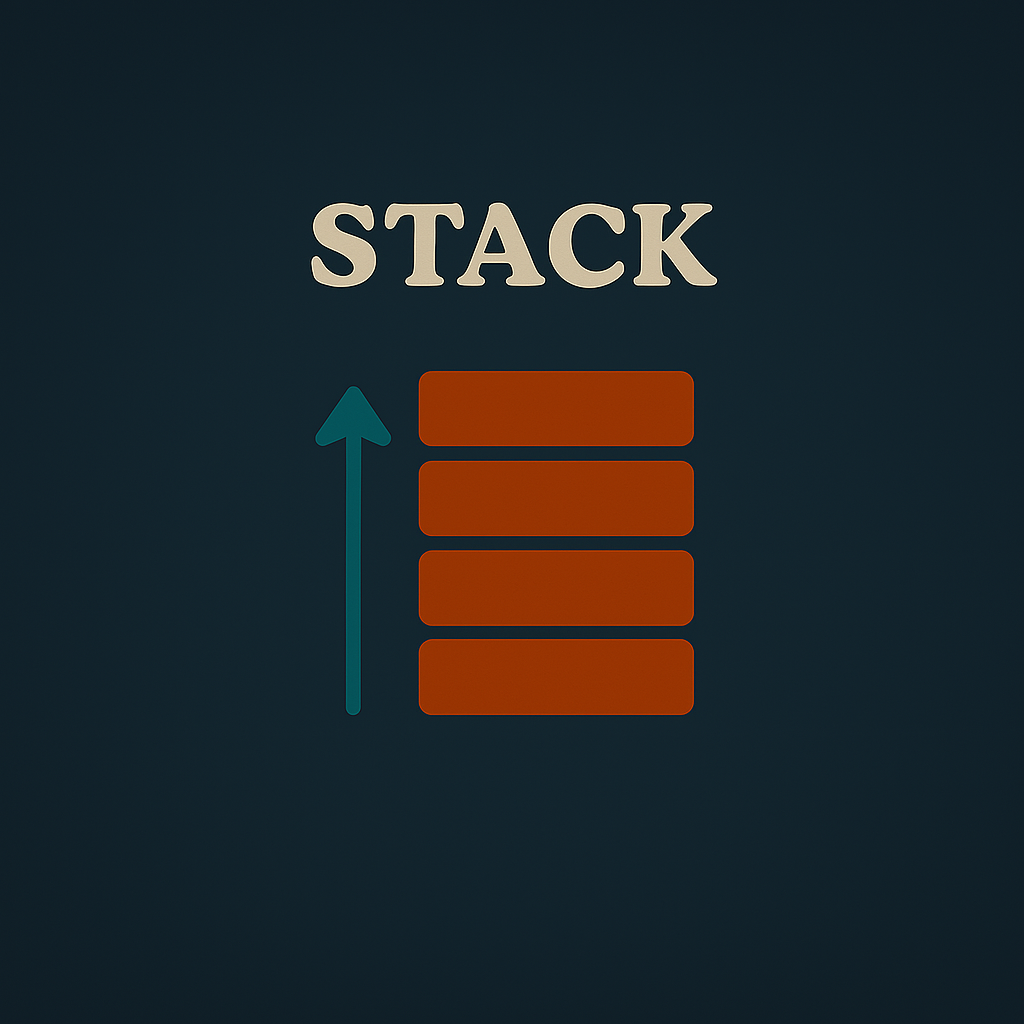
\includegraphics[height=13.88cm, width=17cm, keepaspectratio]{Pics/stack.png}
\end{center}

\chapter{Essential Stack Techniques }
\phantomsection                      % <-- creates a hyperlink anchor
\label{sec:stack}
\begin{itemize}
    \item \textbf{Stack Fundamentals:}
    \begin{itemize}
        \item LIFO principle: Last-In-First-Out behavior
        \item Core operations:
        \begin{itemize}
            \item \texttt{push(item)}: Add to top ($O(1)$)
            \item \texttt{pop()}: Remove from top ($O(1)$)
            \item \texttt{top()/peek()}: Access top element ($O(1)$)
        \end{itemize}
        \item Implementation: 
        \begin{itemize}
            \item Arrays (fixed size)
            \item Dynamic arrays (vectors)
            \item Linked lists (rarely needed)
        \end{itemize}
    \end{itemize}
    
    \item \textbf{Parentheses Validation Patterns:}
    \begin{itemize}
        \item Basic validation:
        \begin{itemize}
            \item Push opening brackets, pop on closing brackets
            \item Check stack empty at end
        \end{itemize}
        \item Complex variants:
        \begin{itemize}
            \item Multiple bracket types (\{\}, [], ())
            \item Minimum add to make valid: Track imbalance count
            \item Score of parentheses: Recursive stack evaluation
        \end{itemize}
    \end{itemize}
    
    \item \textbf{Monotonic Stack Patterns:}
    \begin{itemize}
        \item Next Greater Element (NGE):
        \begin{itemize}
            \item Decreasing stack: Pop while current $>$ stack top
            \item Left NGE: Traverse right-to-left
            \item Circular arrays: Double array length or modulo index
        \end{itemize}
        \item Stock span problem:
        \begin{itemize}
            \item Decreasing stack: Pop while price $>=$ stack top
            \item Span = current index - stack top index
        \end{itemize}
        \item Largest rectangle in histogram:
        \begin{itemize}
            \item Increasing stack: Pop while current $<$ stack top
            \item Area = height[pop] $\times$ (i - stack top - 1)
        \end{itemize}
    \end{itemize}
    
    \item \textbf{Expression Evaluation:}
    \begin{itemize}
        \item Infix to postfix:
        \begin{itemize}
            \item Operator stack + precedence rules
            \item Shunting-yard algorithm
        \end{itemize}
        \item Postfix evaluation:
        \begin{itemize}
            \item Operand stack: Push numbers, pop on operators
            \item Handle unary operators (-, !)
        \end{itemize}
        \item Basic calculator:
        \begin{itemize}
            \item Two stacks: Operands and operators
            \item Handle precedence and parentheses
        \end{itemize}
    \end{itemize}
    
    \item \textbf{Recursion Simulation:}
    \begin{itemize}
        \item DFS traversal:
        \begin{itemize}
            \item Explicit stack replaces recursion
            \item Push (node, state) for complex traversals
        \end{itemize}
        \item Tree traversals:
        \begin{itemize}
            \item Inorder: Push left until null, pop, go right
            \item Preorder: Process node, push right then left
        \end{itemize}
        \item Tower of Hanoi: Track source, destination, auxiliary
    \end{itemize}
    
    \item \textbf{Undo/Redo Operations:}
    \begin{itemize}
        \item Dual stack approach:
        \begin{itemize}
            \item Main stack + undo stack
            \item Redo: Pop from undo, push to main
        \end{itemize}
        \item Text editor operations:
        \begin{itemize}
            \item Store (operation, state) pairs
            \item Support nested undos
        \end{itemize}
    \end{itemize}
    
    \item \textbf{Advanced Stack Techniques:}
    \begin{itemize}
        \item Min/Max stack:
        \begin{itemize}
            \item Dual stack: Main stack + min/max stack
            \item Single stack: Store tuple (value, current-min)
        \end{itemize}
        \item Rainwater trapping:
        \begin{itemize}
            \item Decreasing stack: Compute water between bounds
            \item Alternative: Two-pointer approach
        \end{itemize}
        \item Asteroid collision:
        \begin{itemize}
            \item Push positives, handle negatives by destruction logic
            \item Direction-based collisions
        \end{itemize}
    \end{itemize}
    
    \item \textbf{Hybrid Techniques:}
    \begin{itemize}
        \item Stack + DFS:
        \begin{itemize}
            \item Iterative DFS for trees/graphs
            \item Flood fill with stack
        \end{itemize}
        \item Stack + Math:
        \begin{itemize}
            \item Evaluate RPN with operator functions
            \item Compute nested expressions recursively
        \end{itemize}
        \item Stack + Hashmap:
        \begin{itemize}
            \item Next greater element with value mapping
            \item Valid parentheses with bracket mapping
        \end{itemize}
    \end{itemize}
    
    \item \textbf{Edge Cases \& Pitfalls:}
    \begin{itemize}
        \item Empty stack: Check before pop/peek
        \item Single element stacks
        \item Negative numbers in expression evaluation
        \item Equal elements in monotonic stacks
        \item Circular array boundary conditions
        \item Large input stack overflow (recursive DFS)
    \end{itemize}
    
    \item \textbf{Optimization Strategies:}
    \begin{itemize}
        \item Precomputation:
        \begin{itemize}
            \item Pre-calculate next greater elements
            \item Store prefix max/min arrays
        \end{itemize}
        \item Space optimization:
        \begin{itemize}
            \item Single-stack min/max tracking
            \item Reuse input array as stack
        \end{itemize}
        \item Early termination:
        \begin{itemize}
            \item Invalid parentheses detection
            \item Collision completion detection
        \end{itemize}
    \end{itemize}
    
    \item \textbf{Common Problem Patterns:}
    \begin{itemize}
        \item Daily temperatures: NGE variant
        \item Remove k digits: Monotonic increasing stack
        \item Validate stack sequences: Simulate push/pop
        \item Exclusive time of functions: Stack with timestamps
        \item Decode string: Stack for nested expansions
    \end{itemize}
    
    \item \textbf{Language-Specific Nuances:}
    \begin{itemize}
        \item C++: \texttt{stack} container (no iteration)
        \item Java: \texttt{Stack} class (thread-safe) or \texttt{ArrayDeque}
        \item Python: List as stack (\texttt{append()}, \texttt{pop()})
        \item JavaScript: Array with \texttt{push()}, \texttt{pop()}
    \end{itemize}
    
    \item \textbf{Testing \& Debugging:}
    \begin{itemize}
        \item Small test cases: 0-3 elements
        \item Verify stack state after each operation
        \item Print stack contents in complex algorithms
        \item Boundary tests: Empty input, max size
        \item Monotonic property verification
    \end{itemize}
    
    \item \textbf{When to Use Stack:}
    \begin{itemize}
        \item Nested structures (parentheses, tags)
        \item Nearest greater/smaller element problems
        \item DFS traversal without recursion
        \item Undo/redo functionality
        \item History tracking (browser back button)
        \item Problems requiring LIFO processing
    \end{itemize}
\end{itemize}
\section{Stack-Based DSA Problems Summary Table}
\begin{longtable}{|>{\raggedright\arraybackslash}p{3.2cm}|>{\columncolor{c2}\centering\arraybackslash}p{2.5cm}|>{\columncolor{c3}\raggedright\arraybackslash}p{4.3cm}|>{\columncolor{c4}\raggedright\arraybackslash}p{3.5cm}|>{\columncolor{c5}\color{white}\raggedright\arraybackslash}p{3.5cm}|}
\hline
\rowcolor{rclr}
\textbf{Problem Name} & \textbf{Time Complexity} & \textbf{Idea to Solve} & \textbf{Optimization Tip} & \textbf{Edge Cases} \\
\hline
\endfirsthead

\hline
\textbf{Problem Name} & \textbf{Time Complexity} & \textbf{Idea to Solve} & \textbf{Optimization Tip} & \textbf{Edge Cases} \\
\hline
\endhead
\hline
Balanced Parentheses & $\mathcal{O}(n)$ & Use stack to match opening and closing brackets. & Use map for matching pairs. & Unmatched opening/closing, nested brackets \\
\hline
Sort a Stack & $O(n^2)$ & Use recursion: pop element, sort rest, insert in correct pos recursively. & Simulate with another stack if iterative version needed. & Stack with equal elements or single element \\
\hline
Implement K Stacks in an Array & $\mathcal{O}(1)$ per operation & Use one array + 2 extra arrays (top, next) with free list. & Use space efficiently with linked list logic. & Stack overflow, empty pop \\
\hline
Stock Span Problem & $\mathcal{O}(n)$ & Use stack to track indexes of previous higher values. & Store indices, not values. & All elements increasing/decreasing \\
\hline
Previous Greater Element & $\mathcal{O}(n)$ & Traverse from left, use stack to store elements. & Pop smaller elements for current. & No greater element exists \\
\hline
Next Greater Element & $\mathcal{O}(n)$ & Traverse from right, use stack for next greater. & Reverse loop and build result. & Last element, decreasing order \\
\hline
Largest Rectangular Area in Histogram & $\mathcal{O}(n)$ & Use stack to store indices, calculate area with every pop. & Append 0 at end for flush. & All bars same height, decreasing order \\
\hline
Stack with getMin() in $\mathcal{O}(1)$ & $\mathcal{O}(1)$ & Use auxiliary stack or encode min in main stack. & Push modified value to track min. & All elements same, large range \\
\hline
Sum of Subarray Minimums & $O(n)$ & Use Monotonic Stack to find PLE/NLE and apply contribution: \newline $\text{ans} += arr[i] \cdot (i - prev) \cdot (next - i)$ & Use modulo if result large & Duplicates, strictly decreasing \\
\hline
Remove K Digits to Make Minimum & $O(n)$ & Greedy using Monotonic Stack: remove previous digit if it's greater & Remove from end if needed after stack pass & Leading zeros \\
\hline
Infix to Postfix Conversion & $\mathcal{O}(n)$ & Use stack for operators, precedence and associativity. & Use function for priority comparison. & Parentheses, unary operators \\
\hline
Evaluation of Postfix Expression & $\mathcal{O}(n)$ & Use stack, push operand, evaluate on operator. & Ensure operator has required operands. & Division by zero, invalid postfix \\
\hline
Infix to Prefix Conversion & $\mathcal{O}(n)$ & Reverse infix, convert to postfix, then reverse result. & Use same logic as infix-postfix with reversed precedence. & Nested brackets, invalid format \\
\hline
Evaluation of Prefix Expression & $\mathcal{O}(n)$ & Traverse right to left, use stack for operands. & Evaluate when operator is found. & Invalid expressions \\
\hline
Largest Rectangle with All 1's (Binary Matrix) & $\mathcal{O}(n \cdot m)$ & Convert rows into histogram, use histogram method row-wise. & Reuse logic from histogram problem. & Single row/column, all 0's or all 1's \\
\hline
\end{longtable}
\clearpage
\newgeometry{margin=1in}
% \documentclass[a4paper,10pt]{article}
% \usepackage[utf8]{inputenc}
% \usepackage{geometry}
% \usepackage[table]{xcolor}
% \usepackage{colortbl}
% \usepackage{color,soul}
% \geometry{margin=0.8in}
% \usepackage{xcolor}
% \usepackage{tikz}
% \usepackage{minted}
% \definecolor{bgcolor}{rgb}{0.8, 0.9, 0.5} % 
% \definecolor{bgcolor1}{rgb}{0.95, 0.95, 0.95} % Light Gray
% \definecolor{bgcolor2}{rgb}{0.85, 0.92, 1.0}  % Soft Blue
% \definecolor{bgcolor3}{rgb}{0.9, 0.85, 1.0}   % Light Purple
% \definecolor{bgcolor4}{rgb}{0.95, 0.88, 0.76} % Warm Beige
% \definecolor{bgcolor5}{rgb}{0.8, 0.95, 0.8}   % Gentle Green
% \definecolor{bgcolor6}{rgb}{1.0, 0.87, 0.87}  % Pastel Red
% \definecolor{bgcolor7}{rgb}{0.86, 0.93, 0.83} % Mint Green
% \definecolor{bgcolor8}{rgb}{0.98, 0.85, 0.94} % Soft Pink
% \definecolor{bgcolor9}{rgb}{0.87, 0.94, 0.98} % Sky Blue
% \definecolor{bgcolor10}{rgb}{0.96, 0.96, 0.82} % Pale Yellow
% 
% \begin{document}
% Balanced Parentheses
\noindent\textbf{Problem: Balanced Parentheses}
\begin{minted}[
bgcolor=bgcolor2,
frame=lines,
framesep=5mm,
rulecolor=\color{black},
linenos,
numbersep=5pt,
fontsize=\normalsize
]{python}
def is_valid(s: str) -> bool:
    """
    Checks if parentheses string is balanced.
    Time Complexity: O(n), Space Complexity: O(n)
    """
    stack = []
    mapping = {')': '(', '}': '{', ']': '['}
    
    for char in s:
        if char in mapping:
            top = stack.pop() if stack else '#'
            if mapping[char] != top:
                return False
        else:
            stack.append(char)
    
    return not stack
\end{minted}

\noindent\textbf{Problem: Sort A Stack}
\begin{minted}[
bgcolor=bgcolor4,
frame=lines,
framesep=5mm,
rulecolor=\color{black},
linenos,
numbersep=5pt,
fontsize=\normalsize
]{python}
def sorted_insert(stack, element):
    """Helper function to insert an element into a sorted stack."""
    if not stack or element > stack[-1]:
        stack.append(element)
    else:
        temp = stack.pop()
        sorted_insert(stack, element)
        stack.append(temp)

def sort_stack(stack):
    """Sorts the stack in ascending order using recursion."""
    if stack:
        temp = stack.pop()
        sort_stack(stack)
        sorted_insert(stack, temp)
\end{minted}
% Implement K Stacks in an Array
\noindent\textbf{Problem: Implement K Stacks in an Array}
\begin{minted}[
bgcolor=bgcolor7,
frame=lines,
framesep=5mm,
rulecolor=\color{black},
linenos,
numbersep=5pt,
fontsize=\normalsize
]{python}
class KStacks:
    """
    Efficiently implements K stacks in single array.
    Time Complexity: O(1) for push/pop, Space Complexity: O(n + k)
    """
    def __init__(self, k, n):
        self.k = k  # Number of stacks
        self.n = n  # Total array size
        self.arr = [0] * n  # Storage array
        self.top = [-1] * k  # Top indices for each stack
        self.next_idx = list(range(1, n)) + [-1]  # Next free index
        self.free = 0  # Starting free index

    def push(self, sn, item):
        if self.free == -1:
            raise Exception("Stack overflow")
        
        # Store at current free position
        insert_at = self.free
        self.free = self.next_idx[insert_at]
        self.arr[insert_at] = item
        
        # Update stack pointers
        self.next_idx[insert_at] = self.top[sn]
        self.top[sn] = insert_at

    def pop(self, sn):
        if self.top[sn] == -1:
            raise Exception("Stack underflow")
        
        # Get top element and update pointers
        top_idx = self.top[sn]
        item = self.arr[top_idx]
        self.top[sn] = self.next_idx[top_idx]
        
        # Update free list
        self.next_idx[top_idx] = self.free
        self.free = top_idx
        
        return item
\end{minted}

% Stock Span Problem
\noindent\textbf{Problem: Stock Span Problem}
\begin{minted}[
bgcolor=bgcolor5,
frame=lines,
framesep=5mm,
rulecolor=\color{black},
linenos,
numbersep=5pt,
fontsize=\normalsize
]{python}
def stock_span(prices):
    """
    Calculates span for each day where span = consecutive days before
    where price <= current day.
    Time Complexity: O(n), Space Complexity: O(n)
    """
    n = len(prices)
    stack = []
    span = [1] * n
    
    for i in range(n):
        # Pop smaller elements
        while stack and prices[stack[-1]] <= prices[i]:
            stack.pop()
        
        # Calculate span
        span[i] = i - stack[-1] if stack else i + 1
        stack.append(i)
    
    return span
\end{minted}

% Previous Greater Element
\noindent\textbf{Problem: Previous Greater Element}
\begin{minted}[
bgcolor=bgcolor3,
frame=lines,
framesep=5mm,
rulecolor=\color{black},
linenos,
numbersep=5pt,
fontsize=\normalsize
]{python}
def prev_greater(arr):
    """
    Finds previous greater element for each array element.
    Time Complexity: O(n), Space Complexity: O(n)
    """
    stack = []
    result = [-1] * len(arr)
    
    for i in range(len(arr)):
        while stack and arr[stack[-1]] <= arr[i]:
            stack.pop()
        
        result[i] = arr[stack[-1]] if stack else -1
        stack.append(i)
    
    return result
\end{minted}

% Next Greater Element
\noindent\textbf{Problem: Next Greater Element}
\begin{minted}[
bgcolor=bgcolor8,
frame=lines,
framesep=5mm,
rulecolor=\color{black},
linenos,
numbersep=5pt,
fontsize=\normalsize
]{python}
def next_greater(arr):
    """
    Finds next greater element for each array element.
    Time Complexity: O(n), Space Complexity: O(n)
    """
    stack = []
    result = [-1] * len(arr)
    
    for i in range(len(arr)):
        while stack and arr[stack[-1]] < arr[i]:
            result[stack.pop()] = arr[i]
        stack.append(i)
    
    return result
####################################ALTERNATE#####################################
    def next_greater_from_right(arr):
    """
    Finds next greater element for each array element (right to left traversal).
    Time: O(n), Space: O(n)
    """
    stack = []
    n = len(arr)
    result = [-1] * n

    for i in range(n - 1, -1, -1):
        # Pop smaller or equal elements
        while stack and stack[-1] <= arr[i]:
            stack.pop()

        # Top of stack is the next greater
        if stack:
            result[i] = stack[-1]

        # Push current element for upcoming comparisons
        stack.append(arr[i])

    return result

\end{minted}

% Largest Rectangular Area in Histogram
\noindent\textbf{Problem: Largest Rectangular Area in Histogram}\\
Keep a monotonic increasing stack of indices.When you see a new bar at index i that’s shorter than the bar at the top of the stack, you know:

The popped bar (call its index j) has its right‐first‐smaller at i.

Its left‐first‐smaller is the new top of the stack (after popping).
\begin{minted}[
bgcolor=bgcolor1,
frame=lines,
framesep=5mm,
rulecolor=\color{black},
linenos,
numbersep=5pt,
fontsize=\normalsize
]{python}
def largest_rectangle_area(heights):
    """
    Calculates largest rectangle area in histogram using monotonic stack.
    Time Complexity: O(n), Space Complexity: O(n)
    """
    stack = []
    max_area = 0
    heights.append(0)  # Sentinel value
    
    for i in range(len(heights)):
        while stack and heights[i] < heights[stack[-1]]:
            h = heights[stack.pop()]
            w = i - stack[-1] - 1 if stack else i
            max_area = max(max_area, h * w)
        stack.append(i)
    
    return max_area
\end{minted}

% Stack with getMin() in O(1)
\noindent\textbf{Problem: Stack with getMin() in O(1)}
\begin{minted}[
bgcolor=bgcolor9,
frame=lines,
framesep=5mm,
rulecolor=\color{black},
linenos,
numbersep=5pt,
fontsize=\normalsize
]{python}
class MinStack:
    """
    Implements stack that supports push, pop, top, and getMin in O(1) time.
    Space Complexity: O(n)
    """
    def __init__(self):
        self.stack = []
        self.min_stack = []

    def push(self, val: int) -> None:
        self.stack.append(val)
        if not self.min_stack or val <= self.min_stack[-1]:
            self.min_stack.append(val)

    def pop(self) -> None:
        if self.stack.pop() == self.min_stack[-1]:
            self.min_stack.pop()

    def top(self) -> int:
        return self.stack[-1]

    def getMin(self) -> int:
        return self.min_stack[-1]

################################CONSTANT SPACE #############################

class MinStack:
    def __init__(self):
        self.stack = []
        self.min = None

    def push(self, val: int) -> None:
        if not self.stack:
            self.stack.append(val)
            self.min = val
        elif val >= self.min:
            self.stack.append(val)
        else:
            # Encode the new min in the stack
            self.stack.append(2 * val - self.min)
            self.min = val

    def pop(self) -> None:
        if not self.stack:
            return
        top = self.stack.pop()
        if top < self.min:
            # Decoding previous min
            self.min = 2 * self.min - top

    def top(self) -> int:
        top = self.stack[-1]
        if top >= self.min:
            return top
        else:
            # It’s an encoded value, so actual top is current min
            return self.min

    def getMin(self) -> int:
        return self.min
\end{minted}

% Sum of Subarray Minimums
\noindent\textbf{Problem: Sum of Subarray Minimums}
\begin{minted}[
bgcolor=bgcolor6,
frame=lines,
framesep=5mm,
rulecolor=\color{black},
linenos,
numbersep=5pt,
fontsize=\normalsize
]{python}
def sum_subarray_mins(arr):
    """
    Calculates sum of minimums of all contiguous subarrays.
    Time Complexity: O(n), Space Complexity: O(n)
    """
    MOD = 10**9 + 7
    stack = []
    left = [0] * len(arr)  # Left boundary
    right = [0] * len(arr)  # Right boundary

    # Left boundaries
    for i in range(len(arr)):
        while stack and arr[stack[-1]] > arr[i]:
            stack.pop()
        left[i] = i - stack[-1] if stack else i + 1
        stack.append(i)
    
    stack.clear()
    
    # Right boundaries
    for i in range(len(arr)-1, -1, -1):
        while stack and arr[stack[-1]] >= arr[i]:
            stack.pop()
        right[i] = stack[-1] - i if stack else len(arr) - i
        stack.append(i)
    
    # Calculate total sum
    total = 0
    for i in range(len(arr)):
        total = (total + arr[i] * left[i] * right[i]) % MOD
        
    return total
\end{minted}

% Remove K Digits to Make Minimum
\noindent\textbf{Problem: Remove K Digits to Make Minimum}
\begin{minted}[
bgcolor=bgcolor4,
frame=lines,
framesep=5mm,
rulecolor=\color{black},
linenos,
numbersep=5pt,
fontsize=\normalsize
]{python}
def remove_k_digits(num: str, k: int) -> str:
    """
    Removes k digits to form smallest possible number.
    Time Complexity: O(n), Space Complexity: O(n)
    """
    stack = []
    remain = len(num) - k
    
    for digit in num:
        while k and stack and stack[-1] > digit:
            stack.pop()
            k -= 1
        stack.append(digit)
    
    # If we still have digits to remove (monotonically increasing case)
    while k > 0:
        stack.pop()
        k -= 1
    
    # Remove leading zeros
    res = "".join(stack).lstrip('0')
    return res if res else "0"
\end{minted}

% Infix to Postfix Conversion
\noindent\textbf{Problem: Infix to Postfix Conversion}
\begin{minted}[
bgcolor=bgcolor10,
frame=lines,
framesep=5mm,
rulecolor=\color{black},
linenos,
numbersep=5pt,
fontsize=\normalsize
]{python}
def infix_to_postfix(infix):
    """
    Converts infix expression to postfix using Shunting Yard algorithm.
    Time Complexity: O(n), Space Complexity: O(n)
    """
    precedence = {'+':1, '-':1, '*':2, '/':2, '^':3}
    stack = []
    output = []
    
    for token in infix:
        if token.isalnum():
            output.append(token)
        elif token == '(':
            stack.append(token)
        elif token == ')':
            while stack and stack[-1] != '(':
                output.append(stack.pop())
            stack.pop()  # Remove '('
        else:  # Operator
            while (stack and stack[-1] != '(' and 
                   precedence[token] <= precedence.get(stack[-1], 0)):
                output.append(stack.pop())
            stack.append(token)
    
    while stack:
        output.append(stack.pop())
    
    return ''.join(output)
\end{minted}

% Evaluation of Postfix Expression
\noindent\textbf{Problem: Evaluation of Postfix Expression}
\begin{minted}[
bgcolor=bgcolor2,
frame=lines,
framesep=5mm,
rulecolor=\color{black},
linenos,
numbersep=5pt,
fontsize=\normalsize
]{python}
def eval_postfix(expression):
    """
    Evaluates postfix expression using stack.
    Time Complexity: O(n), Space Complexity: O(n)
    """
    stack = []
    
    for token in expression:
        if token.isdigit():
            stack.append(int(token))
        else:
            b = stack.pop()
            a = stack.pop()
            if token == '+': stack.append(a + b)
            elif token == '-': stack.append(a - b)
            elif token == '*': stack.append(a * b)
            elif token == '/': stack.append(int(a / b))  # Integer division
            elif token == '^': stack.append(a ** b)
    
    return stack[0]
\end{minted}

% Infix to Prefix Conversion
\noindent\textbf{Problem: Infix to Prefix Conversion}
\begin{minted}[
bgcolor=bgcolor7,
frame=lines,
framesep=5mm,
rulecolor=\color{black},
linenos,
numbersep=5pt,
fontsize=\normalsize
]{python}
def infix_to_prefix(infix):
    """
    Converts infix expression to prefix using modified Shunting Yard.
    Time Complexity: O(n), Space Complexity: O(n)
    """
    infix = infix[::-1]  # Reverse infix
    # Swap parentheses
    infix = ''.join([')' if c == '(' else '(' if c == ')' else c for c in infix])
    
    postfix = infix_to_postfix(infix)  # Use our previous function
    return postfix[::-1]  # Reverse postfix to get prefix
\end{minted}

% Evaluation of Prefix Expression
\noindent\textbf{Problem: Evaluation of Prefix Expression}
\begin{minted}[
bgcolor=bgcolor5,
frame=lines,
framesep=5mm,
rulecolor=\color{black},
linenos,
numbersep=5pt,
fontsize=\normalsize
]{python}
def eval_prefix(expression):
    """
    Evaluates prefix expression using stack.
    Time Complexity: O(n), Space Complexity: O(n)
    """
    stack = []
    # Process from right to left
    for token in reversed(expression):
        if token.isdigit():
            stack.append(int(token))
        else:
            a = stack.pop()
            b = stack.pop()
            if token == '+': stack.append(a + b)
            elif token == '-': stack.append(a - b)
            elif token == '*': stack.append(a * b)
            elif token == '/': stack.append(int(a / b))
            elif token == '^': stack.append(a ** b)
    
    return stack[0]
\end{minted}

% Largest Rectangle with All 1's (Binary Matrix)
\noindent\textbf{Problem: Largest Rectangle with All 1's (Binary Matrix)}
\begin{minted}[
bgcolor=bgcolor3,
frame=lines,
framesep=5mm,
rulecolor=\color{black},
linenos,
numbersep=5pt,
fontsize=\normalsize
]{python}
def maximal_rectangle(matrix):
    """
    Finds largest rectangle containing only 1's in binary matrix.
    Time Complexity: O(rows * cols), Space Complexity: O(cols)
    """
    if not matrix:
        return 0
    
    rows, cols = len(matrix), len(matrix[0])
    heights = [0] * cols
    max_area = 0
    
    for i in range(rows):
        # Update heights for current row
        for j in range(cols):
            heights[j] = heights[j] + 1 if matrix[i][j] == '1' else 0
        
        # Calculate max area in histogram
        stack = []
        for j in range(cols + 1):
            while stack and (j == cols or heights[j] < heights[stack[-1]]):
                h = heights[stack.pop()]
                w = j - stack[-1] - 1 if stack else j
                max_area = max(max_area, h * w)
            stack.append(j)
    
    return max_area
\end{minted}

% \end{document}

\newgeometry{margin=0.2in}
\vspace*{47mm}

\begin{center}

{\fontsize{55}{20}\selectfont \textcolor{headingcolor}{\bfseries QUEUE DEQUE}}
\end{center}

\vspace{50mm}

\begin{center}
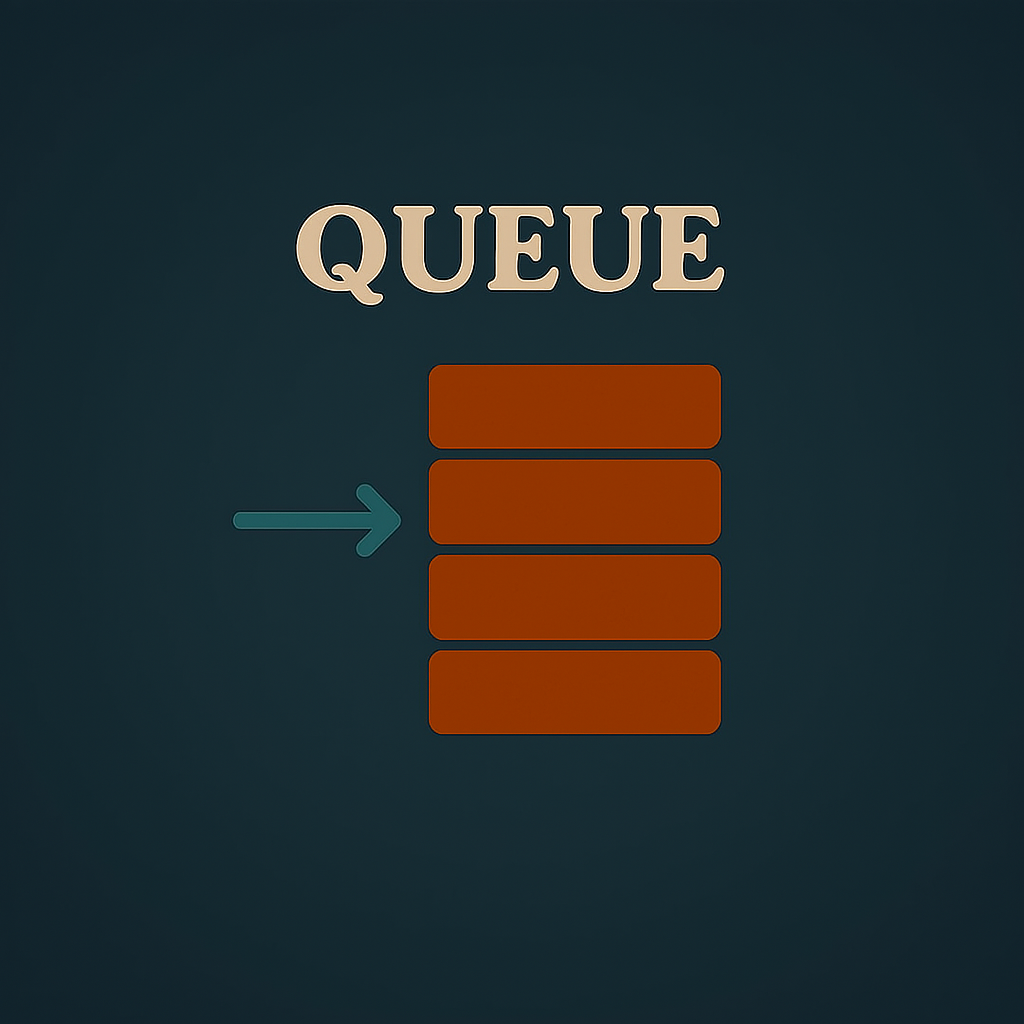
\includegraphics[height=13.88cm, width=17cm, keepaspectratio]{Pics/queue.png}
\end{center}

\chapter{Essential Queue \& Deque Techniques }
\phantomsection                      % <-- creates a hyperlink anchor
\label{sec:queue}
\begin{itemize}
    \item \textbf{Core Concepts:}
    \begin{itemize}
        \item FIFO principle: First-In-First-Out (Queue)
        \item Double-ended operations: Insert/remove at both ends (Deque)
        \item Complexity:
        \begin{itemize}
            \item Enqueue/dequeue: $O(1)$
            \item Access front/rear: $O(1)$
            \item Search: $O(n)$
        \end{itemize}
        \item Implementations:
        \begin{itemize}
            \item Circular arrays (fixed size)
            \item Linked lists (dynamic size)
            \item Language support: \texttt{Queue}, \texttt{Deque} (Python), \texttt{ArrayDeque} (Java), \texttt{deque} (C++)
        \end{itemize}
    \end{itemize}
    
    \item \textbf{Breadth-First Search (BFS):}
    \begin{itemize}
        \item Level-order traversal:
        \begin{itemize}
            \item Process nodes level by level
            \item Queue size = current level nodes
        \end{itemize}
        \item Shortest path in unweighted graphs:
        \begin{itemize}
            \item Maintain distance array
            \item Queue neighbors of current node
        \end{itemize}
        \item Multi-source BFS:
        \begin{itemize}
            \item Initialize queue with multiple sources
            \item Applications: Rotting oranges, nearest gate
        \end{itemize}
    \end{itemize}
    
    \item \textbf{Sliding Window Patterns:}
    \begin{itemize}
        \item Maximum in sliding window:
        \begin{itemize}
            \item Monotonic decreasing deque
            \item Maintain indices: Front always max, remove smaller elements from rear
        \end{itemize}
        \item Minimum in sliding window:
        \begin{itemize}
            \item Monotonic increasing deque
            \item Remove larger elements from rear
        \end{itemize}
        \item First negative in window:
        \begin{itemize}
            \item Deque storing negative indices
            \item Remove indices outside current window
        \end{itemize}
    \end{itemize}
    
    \item \textbf{Deque-Specific Patterns:}
    \begin{itemize}
        \item Palindrome checker:
        \begin{itemize}
            \item Compare front and rear while deque size > 1
        \end{itemize}
        \item Steque (stack + queue):
        \begin{itemize}
            \item Push front (stack), push back (queue)
            \item Implement with single deque
        \end{itemize}
        \item Deque rotation:
        \begin{itemize}
            \item Rotate elements: \texttt{deque.rotate(n)} (Python)
            \item Manual rotation with push/pop
        \end{itemize}
    \end{itemize}
    
    \item \textbf{Scheduling \& Buffering:}
    \begin{itemize}
        \item Task scheduling:
        \begin{itemize}
            \item Round-robin scheduling with queue
            \item Priority queues for weighted scheduling
        \end{itemize}
        \item Producer-consumer pattern:
        \begin{itemize}
            \item Queue as buffer between producers/consumers
            \item Synchronization required in concurrency
        \end{itemize}
        \item Recent counter:
        \begin{itemize}
            \item Maintain queue of timestamps
            \item Evict expired requests from front
        \end{itemize}
    \end{itemize}
    
    \item \textbf{Advanced Algorithms:}
    \begin{itemize}
        \item Binary tree serialization:
        \begin{itemize}
            \item Level-order using queue (BFS)
            \item Handle null nodes explicitly
        \end{itemize}
        \item Snake game:
        \begin{itemize}
            \item Deque representing snake body
            \item Move: Push new head, pop tail (unless growing)
        \end{itemize}
        \item Cache implementations:
        \begin{itemize}
            \item FIFO cache: Queue for eviction order
            \item LRU cache: Deque + hashmap (or doubly linked list)
        \end{itemize}
    \end{itemize}
    
    \item \textbf{Monotonic Queue Techniques:}
    \begin{itemize}
        \item Next greater element (variation):
        \begin{itemize}
            \item Use deque instead of stack
            \item Process elements in sequence
        \end{itemize}
        \item Constrained subsequence sum:
        \begin{itemize}
            \item Deque storing indices of useful values
            \item Maintain decreasing order (max at front)
        \end{itemize}
        \item Shortest subarray with sum at least K:
        \begin{itemize}
            \item Monotonic increasing deque for prefix sums
            \item Remove larger prefix sums from rear
        \end{itemize}
    \end{itemize}
    
    \item \textbf{Hybrid Techniques:}
    \begin{itemize}
        \item Queue + Hashmap:
        \begin{itemize}
            \item First unique character: Store counts + queue
            \item Evict non-unique characters from front
        \end{itemize}
        \item Deque + Stack:
        \begin{itemize}
            \item Implement stack using deque
            \item Implement deque using stacks
        \end{itemize}
        \item Queue + Priority Queue:
        \begin{itemize}
            \item Sliding window median: Two heaps + delayed removal
        \end{itemize}
    \end{itemize}
    
    \item \textbf{Edge Cases \& Pitfalls:}
    \begin{itemize}
        \item Empty queue/deque: Check before pop
        \item Single element operations
        \item Fixed size queues: Overflow handling
        \item Circular queue: Full/empty state detection
        \item Negative numbers in sliding window
        \item Large K in sliding window (K > array size)
        \item Concurrency issues in producer-consumer
    \end{itemize}
    
    \item \textbf{Optimization Strategies:}
    \begin{itemize}
        \item Precomputation:
        \begin{itemize}
            \item Prefix sums for subarray problems
            \item Frequency counts for unique elements
        \end{itemize}
        \item Lazy removal:
        \begin{itemize}
            \item Mark elements as invalid instead of immediate removal
            \item Clean during peek operations
        \end{itemize}
        \item Space efficiency:
        \begin{itemize}
            \item Store indices instead of values
            \item Reuse input array as queue buffer
        \end{itemize}
    \end{itemize}
    
    \item \textbf{Common Problem Patterns:}
    \begin{itemize}
        \item Sliding window maximum: Monotonic deque
        \item Rotting oranges: Multi-source BFS
        \item Design circular queue: Fixed-size implementation
        \item Open the lock: BFS with state transitions
        \item Reveal cards in increasing order: Deque simulation
        \item Gas station circuit: Queue for circular tour
    \end{itemize}
    
    \item \textbf{Language-Specific Nuances:}
    \begin{itemize}
        \item Python:
        \begin{itemize}
            \item \texttt{collections.deque}: Thread-safe, O(1) operations
            \item \texttt{queue.Queue}: Synchronized for threads
        \end{itemize}
        \item Java:
        \begin{itemize}
            \item \texttt{ArrayDeque}: Resizable array, not thread-safe
            \item \texttt{LinkedList}: Implements Deque interface
        \end{itemize}
        \item C++:
        \begin{itemize}
            \item \texttt{std::queue}: Container adapter
            \item \texttt{std::deque}: Random access, efficient push/pop both ends
        \end{itemize}
    \end{itemize}
    
    \item \textbf{Testing \& Debugging:}
    \begin{itemize}
        \item Verify FIFO property with sequential inputs
        \item Check deque operations at both ends
        \item Test empty, single-element, full-capacity states
        \item Validate BFS level tracking
        \item Visualize monotonic deque state during sliding window
    \end{itemize}
    
    \item \textbf{When to Use Queue vs Deque:}
    \begin{itemize}
        \item Queue: Pure FIFO processing (BFS, buffering)
        \item Deque:
        \begin{itemize}
            \item Sliding window min/max
            \item Palindrome processing
            \item Steque (stack + queue) requirements
            \item Efficient front removal in certain algorithms
        \end{itemize}
    \end{itemize}
    
    \item \textbf{Advanced Applications:}
    \begin{itemize}
        \item Work stealing algorithms: Deque per processor
        \item Undo history: Deque for limited history
        \item Graph edge rotation: Deque for efficient edge swapping
    \end{itemize}
\end{itemize}
\section{Queue \& Deque-Based DSA Problems Summary Table}
\begin{longtable}{|>{\raggedright\arraybackslash}p{3.2cm}|>{\columncolor{c2}\centering\arraybackslash}p{2.5cm}|>{\columncolor{c3}\raggedright\arraybackslash}p{4.3cm}|>{\columncolor{c4}\raggedright\arraybackslash}p{3.5cm}|>{\columncolor{c5}\color{white}\raggedright\arraybackslash}p{3.5cm}|}
\hline
\rowcolor{rclr}
\textbf{Problem Name} & \textbf{Time Complexity} & \textbf{Idea to Solve} & \textbf{Optimization Tip} & \textbf{Edge Cases} \\
\hline
\endfirsthead

\hline
\textbf{Problem Name} & \textbf{Time Complexity} & \textbf{Idea to Solve} & \textbf{Optimization Tip} & \textbf{Edge Cases} \\
\hline
\endhead
\hline
Circular Implementation of Queue & $\mathcal{O}(1)$ & Use array with front and rear pointers modulo array size. & Handle full/empty with count or extra space. & Queue full vs empty detection \\
\hline
Implementing Stack using Queue & Push: $\mathcal{O}(n)$, Pop: $\mathcal{O}(1)$ & Use 2 queues or rotate in single queue during push. & Push elements to maintain LIFO order. & Popping from empty stack \\
\hline
Implementing Queue using Single Stack & $\mathcal{O}(n)$ amortized & Use recursion to simulate queue behavior. & Use function call stack as helper. & Stack overflow, empty queue \\
\hline
Reversing First K Elements of a Queue & $\mathcal{O}(n)$ & Use stack to reverse first k, then enqueue back. & Use queue rotation for remaining elements. & k $>$ size, k = 0 or size \\
\hline
Sliding Window Maximum & $\mathcal{O}(n)$ & Use deque to maintain decreasing order of indices. & Remove out-of-window and smaller elements. & All elements equal or decreasing \\
\hline
Generate Numbers with Given Digits Only & $\mathcal{O}(n)$ & Use queue to generate using BFS (e.g., only {5,6}). & Enqueue number + each digit. & Handle leading zeros \\
\hline
Circular Implementation of Deque & $\mathcal{O}(1)$ & Use circular array with front and rear pointers. & Wrap around using modulo. & Full/empty condition handling \\
\hline
First Circular Tour (Gas Station Problem) & $\mathcal{O}(n)$ & Use two pointers or one-pass tracking surplus. & Start from station with net positive gas. & No solution exists \\
\hline
Design a Data Structure with Min and Max & $\mathcal{O}(1)$ per op & Use deque for max and min separately. & Sync with actual queue insertions/deletions. & Same elements, all increasing/decreasing \\
\hline
\end{longtable}
\clearpage
\newgeometry{margin=1in}
% \documentclass[a4paper,10pt]{article}
% \usepackage[utf8]{inputenc}
% \usepackage{geometry}
% \usepackage[table]{xcolor}
% \usepackage{colortbl}
% \usepackage{color,soul}
% \geometry{margin=0.8in}
% \usepackage{xcolor}
% \usepackage{tikz}
% \usepackage{minted}
% \definecolor{bgcolor}{rgb}{0.8, 0.9, 0.5} % 
% \definecolor{bgcolor1}{rgb}{0.95, 0.95, 0.95} % Light Gray
% \definecolor{bgcolor2}{rgb}{0.85, 0.92, 1.0}  % Soft Blue
% \definecolor{bgcolor3}{rgb}{0.9, 0.85, 1.0}   % Light Purple
% \definecolor{bgcolor4}{rgb}{0.95, 0.88, 0.76} % Warm Beige
% \definecolor{bgcolor5}{rgb}{0.8, 0.95, 0.8}   % Gentle Green
% \definecolor{bgcolor6}{rgb}{1.0, 0.87, 0.87}  % Pastel Red
% \definecolor{bgcolor7}{rgb}{0.86, 0.93, 0.83} % Mint Green
% \definecolor{bgcolor8}{rgb}{0.98, 0.85, 0.94} % Soft Pink
% \definecolor{bgcolor9}{rgb}{0.87, 0.94, 0.98} % Sky Blue
% \definecolor{bgcolor10}{rgb}{0.96, 0.96, 0.82} % Pale Yellow
% 
% \begin{document}
% Circular Queue Implementation
\noindent\textbf{Problem: Circular Implementation of Queue}
\begin{minted}[
bgcolor=bgcolor4,
frame=lines,
framesep=5mm,
rulecolor=\color{black},
linenos,
numbersep=5pt,
fontsize=\normalsize
]{python}
class CircularQueue:
    """
    Circular queue implementation with fixed capacity.
    Time Complexity: O(1) for all operations, Space Complexity: O(n)
    """
    def __init__(self, capacity: int):
        self.capacity = capacity
        self.queue = [None] * capacity
        self.front = self.rear = -1
        self.size = 0

    def enqueue(self, value: int) -> bool:
        if self.is_full():
            return False
            
        if self.is_empty():
            self.front = self.rear = 0
        else:
            self.rear = (self.rear + 1) % self.capacity
            
        self.queue[self.rear] = value
        self.size += 1
        return True

    def dequeue(self) -> bool:
        if self.is_empty():
            return False
            
        if self.front == self.rear:
            self.front = self.rear = -1
        else:
            self.front = (self.front + 1) % self.capacity
            
        self.size -= 1
        return True

    def get_front(self) -> int:
        return -1 if self.is_empty() else self.queue[self.front]

    def get_rear(self) -> int:
        return -1 if self.is_empty() else self.queue[self.rear]

    def is_empty(self) -> bool:
        return self.size == 0

    def is_full(self) -> bool:
        return self.size == self.capacity
\end{minted}

% Stack using Queue
\noindent\textbf{Problem: Implementing Stack using Queue}
\begin{minted}[
bgcolor=bgcolor7,
frame=lines,
framesep=5mm,
rulecolor=\color{black},
linenos,
numbersep=5pt,
fontsize=\normalsize
]{python}
from collections import deque

class StackUsingQueue:
    """
    Stack implementation using two queues.
    Time Complexity: 
        Push: O(1), Pop: O(n), 
        Top: O(1), Empty: O(1)
    """
    def __init__(self):
        self.main = deque()
        self.aux = deque()

    def push(self, x: int) -> None:
        self.main.append(x)

    def pop(self) -> int:
        # Move all except last to auxiliary queue
        while len(self.main) > 1:
            self.aux.append(self.main.popleft())
        
        # Remove and return last element
        val = self.main.popleft()
        
        # Swap queues
        self.main, self.aux = self.aux, self.main
        return val

    def top(self) -> int:
        return self.main[-1] if self.main else -1

    def empty(self) -> bool:
        return len(self.main) == 0
\end{minted}

% Queue using Single Stack
\noindent\textbf{Problem: Implementing Queue using Single Stack}
\begin{minted}[
bgcolor=bgcolor5,
frame=lines,
framesep=5mm,
rulecolor=\color{black},
linenos,
numbersep=5pt,
fontsize=\normalsize
]{python}
class QueueUsingStack:
    """
    Queue implementation using two stacks (single stack in interface).
    Time Complexity: 
        Enqueue: O(1), Dequeue: Amortized O(1)
    """
    def __init__(self):
        self.in_stack = []
        self.out_stack = []

    def enqueue(self, x: int) -> None:
        self.in_stack.append(x)

    def dequeue(self) -> int:
        if not self.out_stack:
            while self.in_stack:
                self.out_stack.append(self.in_stack.pop())
        return self.out_stack.pop() if self.out_stack else -1

    def peek(self) -> int:
        if not self.out_stack:
            while self.in_stack:
                self.out_stack.append(self.in_stack.pop())
        return self.out_stack[-1] if self.out_stack else -1

    def empty(self) -> bool:
        return not self.in_stack and not self.out_stack
\end{minted}

% Reverse First K Elements of Queue
\noindent\textbf{Problem: Reversing First K Elements of a Queue}
\begin{minted}[
bgcolor=bgcolor3,
frame=lines,
framesep=5mm,
rulecolor=\color{black},
linenos,
numbersep=5pt,
fontsize=\normalsize
]{python}
from collections import deque

def reverse_k(queue: deque, k: int) -> deque:
    """
    Reverses first k elements of a queue using stack.
    Time Complexity: O(n), Space Complexity: O(k)
    """
    if k > len(queue) or k <= 0:
        return queue
        
    stack = []
    # Push first k elements to stack
    for _ in range(k):
        stack.append(queue.popleft())
    
    # Pop from stack to end of queue (reversed order)
    while stack:
        queue.append(stack.pop())
    
    # Move remaining elements to end
    for _ in range(len(queue) - k):
        queue.append(queue.popleft())
        
    return queue
\end{minted}

% Sliding Window Maximum
\noindent\textbf{Problem: Sliding Window Maximum}
\begin{minted}[
bgcolor=bgcolor8,
frame=lines,
framesep=5mm,
rulecolor=\color{black},
linenos,
numbersep=5pt,
fontsize=\normalsize
]{python}
from collections import deque

def max_sliding_window(nums: List[int], k: int) -> List[int]:
    """
    Finds max in each sliding window using monotonic deque.
    Time Complexity: O(n), Space Complexity: O(k)
    """
    dq = deque()
    result = []
    
    for i in range(len(nums)):
        # Remove indices outside current window
        if dq and dq[0] == i - k:
            dq.popleft()
            
        # Maintain decreasing order
        while dq and nums[dq[-1]] < nums[i]:
            dq.pop()
            
        dq.append(i)
        
        # Add to result once window size reached
        if i >= k - 1:
            result.append(nums[dq[0]])
    
    return result
\end{minted}

% Generate Numbers with Given Digits
\noindent\textbf{Problem: Generate Numbers with Given Digits Only}
\begin{minted}[
bgcolor=bgcolor1,
frame=lines,
framesep=5mm,
rulecolor=\color{black},
linenos,
numbersep=5pt,
fontsize=\normalsize
]{python}
from collections import deque

def generate_numbers(digits: List[int], n: int) -> List[int]:
    """
    Generates first n numbers containing only given digits.
    Time Complexity: O(n), Space Complexity: O(n)
    """
    result = []
    queue = deque()
    # Start with each digit
    for d in sorted(digits):
        queue.append(d)
    
    count = 0
    while queue and count < n:
        num = queue.popleft()
        result.append(num)
        count += 1
        
        # Generate next numbers by appending digits
        for d in sorted(digits):
            new_num = num * 10 + d
            queue.append(new_num)
    
    return result
\end{minted}

% Circular Deque Implementation
\noindent\textbf{Problem: Circular Implementation of Deque}
\begin{minted}[
bgcolor=bgcolor9,
frame=lines,
framesep=5mm,
rulecolor=\color{black},
linenos,
numbersep=5pt,
fontsize=\normalsize
]{python}
class CircularDeque:
    """
    Circular deque implementation with O(1) operations.
    Space Complexity: O(n)
    """
    def __init__(self, k: int):
        self.capacity = k
        self.deque = [None] * k
        self.front = self.rear = -1
        self.size = 0

    def insert_front(self, value: int) -> bool:
        if self.is_full():
            return False
            
        if self.is_empty():
            self.front = self.rear = 0
        else:
            self.front = (self.front - 1) % self.capacity
            
        self.deque[self.front] = value
        self.size += 1
        return True

    def insert_last(self, value: int) -> bool:
        if self.is_full():
            return False
            
        if self.is_empty():
            self.front = self.rear = 0
        else:
            self.rear = (self.rear + 1) % self.capacity
            
        self.deque[self.rear] = value
        self.size += 1
        return True

    def delete_front(self) -> bool:
        if self.is_empty():
            return False
            
        if self.front == self.rear:
            self.front = self.rear = -1
        else:
            self.front = (self.front + 1) % self.capacity
            
        self.size -= 1
        return True

    def delete_last(self) -> bool:
        if self.is_empty():
            return False
            
        if self.front == self.rear:
            self.front = self.rear = -1
        else:
            self.rear = (self.rear - 1) % self.capacity
            
        self.size -= 1
        return True

    def get_front(self) -> int:
        return -1 if self.is_empty() else self.deque[self.front]

    def get_rear(self) -> int:
        return -1 if self.is_empty() else self.deque[self.rear]

    def is_empty(self) -> bool:
        return self.size == 0

    def is_full(self) -> bool:
        return self.size == self.capacity
\end{minted}

% Gas Station Problem
\noindent\textbf{Problem: First Circular Tour (Gas Station Problem)}
\begin{minted}[
bgcolor=bgcolor6,
frame=lines,
framesep=5mm,
rulecolor=\color{black},
linenos,
numbersep=5pt,
fontsize=\normalsize
]{python}
def can_complete_circuit(gas: List[int], cost: List[int]) -> int:
    """
    Finds starting gas station index to complete circular tour.
    Time Complexity: O(n), Space Complexity: O(1)
    """
    total_tank = current_tank = start = 0
    
    for i in range(len(gas)):
        total_tank += gas[i] - cost[i]
        current_tank += gas[i] - cost[i]
        
        # If current tank negative, reset from next station
        if current_tank < 0:
            start = i + 1
            current_tank = 0
    
    return start if total_tank >= 0 else -1
\end{minted}

% Min-Max Data Structure
\noindent\textbf{Problem: Design a Data Structure with Min and Max}
\begin{minted}[
bgcolor=bgcolor4,
frame=lines,
framesep=5mm,
rulecolor=\color{black},
linenos,
numbersep=5pt,
fontsize=\normalsize
]{python}
from collections import deque

class MinMaxDeque:
    """
    Deque that supports O(1) min/max operations using auxiliary deques.
    Time Complexity: All operations O(1) amortized.
    """
    def __init__(self):
        self.main = deque()
        self.min_deque = deque()
        self.max_deque = deque()

    def append(self, x: int) -> None:
        self.main.append(x)
        # Maintain min deque (increasing)
        while self.min_deque and self.min_deque[-1] > x:
            self.min_deque.pop()
        self.min_deque.append(x)
        # Maintain max deque (decreasing)
        while self.max_deque and self.max_deque[-1] < x:
            self.max_deque.pop()
        self.max_deque.append(x)

    def popleft(self) -> int:
        if not self.main:
            return -1
        val = self.main.popleft()
        if val == self.min_deque[0]:
            self.min_deque.popleft()
        if val == self.max_deque[0]:
            self.max_deque.popleft()
        return val

    def pop(self) -> int:
        if not self.main:
            return -1
        val = self.main.pop()
        if val == self.min_deque[-1]:
            self.min_deque.pop()
        if val == self.max_deque[-1]:
            self.max_deque.pop()
        return val

    def get_min(self) -> int:
        return self.min_deque[0] if self.min_deque else -1

    def get_max(self) -> int:
        return self.max_deque[0] if self.max_deque else -1
\end{minted}

% \end{document}

\newgeometry{margin=0.2in}
\vspace*{47mm}

\begin{center}

{\fontsize{55}{20}\selectfont \textcolor{headingcolor}{\bfseries TREE \& BST}}
\end{center}

\vspace{50mm}

\begin{center}
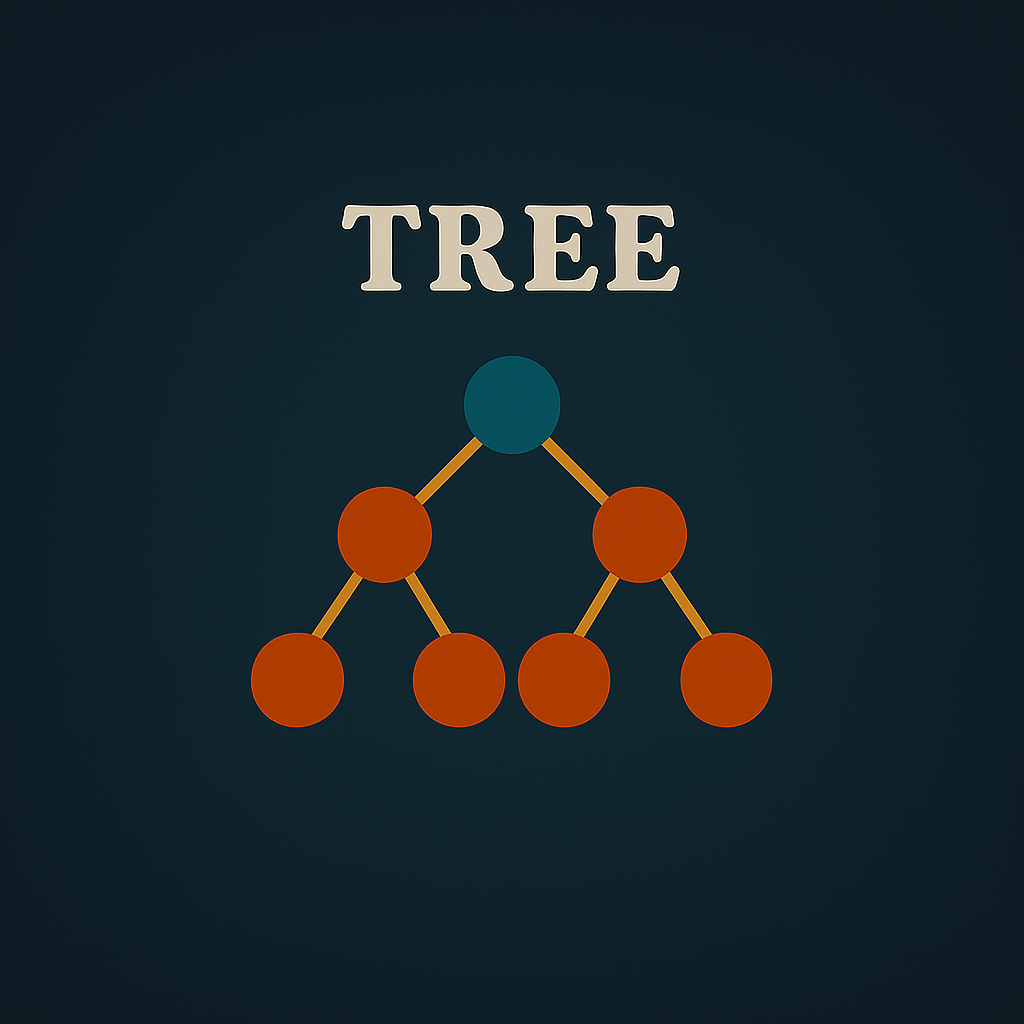
\includegraphics[height=13.88cm, width=17cm, keepaspectratio]{Pics/tree.png}
\end{center}

\chapter{Essential Tree \& BST Techniques }
\phantomsection                      % <-- creates a hyperlink anchor
\label{sec:tree}
\begin{itemize}
    \item \textbf{Core Concepts:}
    \begin{itemize}
        \item Tree properties:
        \begin{itemize}
            \item $n$ nodes $\Rightarrow$ $n-1$ edges
            \item Height: $h = O(\log n)$ (balanced), $O(n)$ (unbalanced)
            \item BST invariant: $\text{left} < \text{root} < \text{right}$
        \end{itemize}
        \item Representations:
        \begin{itemize}
            \item Node-based: \texttt{TreeNode(val, left, right)}
            \item Array-based: Index $i \rightarrow$ children at $2i+1, 2i+2$
        \end{itemize}
    \end{itemize}
    
    \item \textbf{Traversal Techniques:}
    \begin{itemize}
        \item Depth-First Search (DFS):
        \begin{itemize}
            \item Preorder: Root $\rightarrow$ Left $\rightarrow$ Right
            \item Inorder: Left $\rightarrow$ Root $\rightarrow$ Right (BST $\rightarrow$ sorted)
            \item Postorder: Left $\rightarrow$ Right $\rightarrow$ Root
        \end{itemize}
        \item Breadth-First Search (BFS):
        \begin{itemize}
            \item Level-order: Queue-based, $O(n)$
            \item Reverse level-order: Process from bottom
        \end{itemize}
        \item Morris traversal: $O(1)$ space (threaded trees)
    \end{itemize}
    
    \item \textbf{Binary Tree Patterns:}
    \begin{itemize}
        \item Path problems:
        \begin{itemize}
            \item Root-to-leaf paths: DFS with backtracking
            \item Path sum: Target sum checks
            \item Maximum path sum: Postorder with max gain
        \end{itemize}
        \item View problems:
        \begin{itemize}
            \item Left/right view: BFS tracking first/last node
            \item Top/bottom view: Vertical order + offset tracking
        \end{itemize}
        \item Ancestor problems:
        \begin{itemize}
            \item LCA: Recursive search for both nodes
            \item BST LCA: Use BST property to prune
        \end{itemize}
    \end{itemize}
    
    \item \textbf{Binary Search Tree Patterns:}
    \begin{itemize}
        \item Validation:
        \begin{itemize}
            \item Inorder traversal $\rightarrow$ sorted check
            \item Range propagation: $(\min, \max)$ per node
        \end{itemize}
        \item Modification:
        \begin{itemize}
            \item Insert: Find appropriate leaf position
            \item Delete: Handle 0, 1, and 2 children cases
            \item BST to balanced BST: Inorder $\rightarrow$ rebuild
        \end{itemize}
        \item Order statistics:
        \begin{itemize}
            \item Kth smallest: Inorder with counter
            \item Size tracking: Augment node with subtree size
        \end{itemize}
    \end{itemize}
    
    \item \textbf{Advanced Tree Algorithms:}
    \begin{itemize}
        \item Tree building:
        \begin{itemize}
            \item Preorder+Inorder $\rightarrow$ Binary tree
            \item Sorted array $\rightarrow$ Balanced BST
        \end{itemize}
        \item Serialization/Deserialization:
        \begin{itemize}
            \item BFS with null markers
            \item Preorder with special characters
        \end{itemize}
        \item Subtree problems:
        \begin{itemize}
            \item Subtree of Another Tree: Compare all nodes
            \item Merkle hashing: $O(n+m)$ subtree comparison
        \end{itemize}
    \end{itemize}
    
    \item \textbf{Tree Augmentation:}
    \begin{itemize}
        \item Subtree sum: Update on insert/delete
        \item Lazy propagation: Batch updates for range queries
        \item AVL/RB trees: Height balancing rotations
    \end{itemize}
    
    \item \textbf{Special Tree Types:}
    \begin{itemize}
        \item Trie (Prefix tree):
        \begin{itemize}
            \item Word search: Store characters on edges
            \item Applications: Autocomplete, IP routing
        \end{itemize}
        \item Fenwick Tree (Binary Indexed Tree):
        \begin{itemize}
            \item Point updates, prefix sums in $O(\log n)$
            \item Convert array to frequency tree
        \end{itemize}
        \item Segment Tree:
        \begin{itemize}
            \item Range queries: Sum/min/max in $O(\log n)$
            \item Lazy propagation for range updates
        \end{itemize}
    \end{itemize}
    
    \item \textbf{Optimization Strategies:}
    \begin{itemize}
        \item Memoization: Cache subtree results
        \item Pruning: Early termination in DFS
        \item Iterative DFS: Avoid recursion overhead
        \item Path compression: In union-find trees
    \end{itemize}
    
    \item \textbf{Edge Cases \& Pitfalls:}
    \begin{itemize}
        \item Empty tree (null root)
        \item Single node tree
        \item Skewed trees (performance degradation)
        \item Duplicate values in BST (define policy)
        \item Integer overflow in large trees
        \item Cyclic graphs (non-tree inputs)
    \end{itemize}
    
    \item \textbf{Common Problem Patterns:}
    \begin{itemize}
        \item Validate BST: Range propagation
        \item BST iterator: Stack-based DFS
        \item Inorder successor: BST property navigation
        \item House robber III: Tree DP (take/skip)
        \item Symmetric tree: Mirror comparison
    \end{itemize}
    
    \item \textbf{Tree DP Patterns:}
    \begin{itemize}
        \item Diameter of tree: $\max(\text{left}+\text{right})$
        \item Maximum path sum: Postorder with max gain
        \item Tree coloring: Min cameras/guards
        \item Isomorphism: Compare structures recursively
    \end{itemize}
    
    \item \textbf{Hybrid Techniques:}
    \begin{itemize}
        \item BFS + HashMap: Vertical order traversal
        \item DFS + Stack: Iterative traversals
        \item Tree + Two pointers: BST two-sum
        \item BST + Binary search: Kth smallest
    \end{itemize}
    
    \item \textbf{Testing \& Debugging:}
    \begin{itemize}
        \item Small trees: 0-3 nodes
        \item Skewed trees: Left/right chains
        \item Complete trees: All levels filled
        \item Duplicate value handling
        \item Visualization tools: Graphviz output
    \end{itemize}
\end{itemize}
\section{Tree-Based DSA Problems Summary Table}
\begin{longtable}{|>{\raggedright\arraybackslash}p{3.2cm}|>{\columncolor{c2}\centering\arraybackslash}p{2.5cm}|>{\columncolor{c3}\raggedright\arraybackslash}p{4.3cm}|>{\columncolor{c4}\raggedright\arraybackslash}p{3.5cm}|>{\columncolor{c5}\color{white}\raggedright\arraybackslash}p{3.5cm}|}
\hline
\rowcolor{rclr}
\textbf{Problem Name} & \textbf{Time Complexity} & \textbf{Idea to Solve} & \textbf{Optimization Tip} & \textbf{Edge Cases} \\
\hline
\endfirsthead

\hline
\rowcolor{rclr}
\textbf{Problem Name} & \textbf{Time Complexity} & \textbf{Idea to Solve} & \textbf{Optimization Tip} & \textbf{Edge Cases} \\
\hline
\endhead
Iterative Inorder Traversal & $\mathcal{O}(n)$ & Use stack to simulate recursion. Push left nodes, then visit right. & Use controlled while loop with current node and stack. & Empty tree, single node \\
\hline
Iterative Preorder Traversal & $\mathcal{O}(h)$ & Use stack, push right first, then left. & Avoid putting left on stack just put right after processing left. & Left-skewed or right-skewed tree \\
\hline
Iterative Postorder Traversal & $\mathcal{O}(n)$ & Use two stacks or one stack with visited flag. & Reverse modified preorder (root-right-left). & Single node, skewed tree \\
\hline
Threaded Binary Tree Inorder Traversal & $\mathcal{O}(n)$ & Use right threads for successors, avoid recursion/stack. & Morris traversal modifies tree temporarily. & No left/right child, restore tree \\
\hline
Pre, In, Post Order in Single DFS & $O(n)$ & Use stack and state tracking (1: pre, 2: in, 3: post) per node & Push state-tuple to stack instead of recursion & Empty tree \\
\hline
Pre, In, Post Order via BFS & $O(n)$ & Not standard — simulate by storing BFS with level and direction info & Mainly used for printing levels differently & Level-wise variant only \\
\hline
Morris Inorder Traversal & $O(n)$ & Use threaded tree (predecessor’s right = current), no stack/recursion & Restore tree links after traversal & Tree with only right nodes \\
\hline
Morris Preorder Traversal & $O(n)$ & Same as inorder but print before going to left subtree & Restore links carefully & Skewed trees \\
\hline
Level Order Traversal & $\mathcal{O}(n)$ & Use queue for BFS traversal by levels. & Track level ends with size or marker. & Empty tree \\
\hline
Left, Right, Top, Bottom View of Tree & $\mathcal{O}(n)$ & Use queue + map for horizontal distance or level. & Track first/last node at each level or HD. & Nodes at same level or HD \\
\hline
Check for Balanced Binary Tree & $\mathcal{O}(n)$ & Recursively get height and check balance. & Return -1 early if unbalanced. & Perfectly skewed tree \\
\hline
Maximum Width of Binary Tree & $\mathcal{O}(n)$ & Level order with index tracking for each node. & Normalize indices per level to avoid overflow. & Tree with missing internal nodes \\
\hline
Construct Tree from Inorder and Preorder & $\mathcal{O}(n)$ & Use preorder index and map for inorder positions. & Use hashmap to speed up root index lookup. & Invalid or repeated values \\
\hline
Tree Traversal in Spiral Form & $\mathcal{O}(n)$ & Use two stacks or deque to alternate direction. & Use direction flag to control insertion. & Skewed trees \\
\hline
Child Sum Property in Tree & $\mathcal{O}(n)$ & Check if node value = sum of children recursively. & Leaf node automatically satisfies. & Null children, 0 values \\
\hline
Convert Binary Tree to Doubly Linked List & $\mathcal{O}(n)$ & Inorder traversal with prev pointer to link nodes. & Use static/global prev pointer. & Single node, skewed trees \\
\hline
Convert Binary Tree to Singly Linked List & $\mathcal{O}(n)$ & Preorder traversal and right-only links. & Recursively attach left-subtree to right. & All left children \\
\hline
Finding LCA in Binary Tree & $\mathcal{O}(n)$ & Recursively return current node if matches either, else combine. & Return ancestor if both sides return non-null. & LCA is one of the nodes \\
\hline
Burn a Binary Tree From a Leaf & $\mathcal{O}(n)$ & Use BFS and parent map, simulate fire spreading level-wise. & Build parent links first, then run BFS. & Leaf is root, isolated nodes \\
\hline
Serialize and Deserialize Binary Tree & $\mathcal{O}(n)$ & Use preorder with NULL markers or level order. & Use delimiter or marker for NULLs. & NULL-heavy or skewed tree \\
\hline
Insertion in Binary Tree & $\mathcal{O}(n)$ & Level order traversal, insert at first empty left/right. & Use queue to find first incomplete node. & Tree is full, insertion at root \\
\hline
Deletion in Binary Tree & $\mathcal{O}(n)$ & Replace target with deepest node, then delete deepest. & Track parent of deepest separately. & Node not found, deleting root \\
\hline
Convert Binary Tree into Mirror Tree & $\mathcal{O}(n)$ & Recursively swap left and right subtrees. & Post-order traversal ensures bottom-up swap. & Symmetric trees \\
\hline
Count Nodes in Complete Binary Tree & $\mathcal{O}(\log^2 n)$ & Use height comparison of left and right subtrees. & Apply binary search if needed. & Perfect or skewed tree \\
\hline
Diameter of a Binary Tree & $\mathcal{O}(n)$ & Recursively compute height + update diameter at each node. & Store height in return to avoid recomputation. & Tree with only left/right nodes \\
\hline
Max Path Sum (Any Node to Any Node) & $O(n)$ & At each node: return max(root, root + L, root + R), update global max as $\max(global, root + L + R)$ & Use postorder and maintain global max & All negative nodes (return max node) \\
\hline
Max Path Sum Leaf to Leaf & $O(n)$ & If both children exist: update global as $L + R + root$, return max(L, R) + root & Handle leaf-only subtree separately & Single child nodes, leaf = root \\
\hline
Count All Paths with Given Sum in Binary Tree & $O(n)$ & Prefix sum + hashmap: count paths where sum(curr) - target exists in map. & Backtrack prefix sum count while unwinding recursion. & Negative values, path not from root \\
\hline
Diameter of N-ary Tree & $O(n)$ & At each node, store 2 largest child heights, update diameter as $h1 + h2 + 1$ & Maintain global diameter in postorder traversal & Single node or single branch \\
\hline
Boundary Traversal of Binary Tree & $O(n)$ & Print root → left boundary (non-leaf) → leaves → right boundary (reverse) & Handle duplicates of leaf nodes properly & Single node / skewed tree \\
\hline
Child Sum Property & $O(n)$ & Modify tree: for each node, make child sum = node value recursively & Update child or node as needed to preserve invariant & Leaf node base case \\
\hline
Burning Tree from a Leaf & $O(n)$ & Use parent map + BFS from the leaf node to simulate burn time level-wise & Track visited to avoid reprocessing & Leaf not existing or multiple leaves \\
\hline
Binary Tree to Linked List (Morris-based) & $O(n)$ & Morris + rearrange right pointers during preorder visit & Use a dummy node or prev tracker & Single node or all left nodes \\
\hline
\end{longtable}
\clearpage
\newgeometry{margin=1in}
% \documentclass[a4paper,10pt]{article}
% \usepackage[utf8]{inputenc}
% \usepackage{geometry}
% \usepackage[table]{xcolor}
% \usepackage{colortbl}
% \usepackage{color,soul}
% \geometry{margin=0.8in}
% \usepackage{xcolor}
% \usepackage{tikz}
% \usepackage{minted}
% \definecolor{bgcolor}{rgb}{0.8, 0.9, 0.5} % 
% \definecolor{bgcolor1}{rgb}{0.95, 0.95, 0.95} % Light Gray
% \definecolor{bgcolor2}{rgb}{0.85, 0.92, 1.0}  % Soft Blue
% \definecolor{bgcolor3}{rgb}{0.9, 0.85, 1.0}   % Light Purple
% \definecolor{bgcolor4}{rgb}{0.95, 0.88, 0.76} % Warm Beige
% \definecolor{bgcolor5}{rgb}{0.8, 0.95, 0.8}   % Gentle Green
% \definecolor{bgcolor6}{rgb}{1.0, 0.87, 0.87}  % Pastel Red
% \definecolor{bgcolor7}{rgb}{0.86, 0.93, 0.83} % Mint Green
% \definecolor{bgcolor8}{rgb}{0.98, 0.85, 0.94} % Soft Pink
% \definecolor{bgcolor9}{rgb}{0.87, 0.94, 0.98} % Sky Blue
% \definecolor{bgcolor10}{rgb}{0.96, 0.96, 0.82} % Pale Yellow
% 
% % Define a custom background colo
% \begin{document}
\noindent\textbf{Problem: Iterative Inorder Traversal}
\begin{minted}[
bgcolor=bgcolor7,
frame=lines,
framesep=5mm,
rulecolor=\color{black},
linenos,
numbersep=5pt,
fontsize=\normalsize
]{python}
class TreeNode:
    def __init__(self, val=0, left=None, right=None):
        self.val = val
        self.left = left
        self.right = right

def inorder_traversal(root: TreeNode) -> List[int]:
    """
    Performs iterative inorder traversal of a binary tree.
    Time Complexity: O(n)      Space Complexity: O(n)
    """
    stack = []
    result = []
    current = root
    
    while current or stack:
        # Traverse to the leftmost node
        while current:
            stack.append(current)
            current = current.left
        # Process the node at the top of the stack
        current = stack.pop()
        result.append(current.val)
        # Move to the right subtree
        current = current.right
    
    return result
\end{minted}

\noindent\textbf{Problem: Iterative Preorder Traversal}
\begin{minted}[
bgcolor=bgcolor2,
frame=lines,
framesep=5mm,
rulecolor=\color{black},
linenos,
numbersep=5pt,
fontsize=\normalsize
]{python}
def preorder_traversal(root: TreeNode) -> List[int]:
    """
    Performs iterative preorder traversal of a binary tree.
    Time Complexity: O(n)      Space Complexity: O(n)
    """
    if not root:
        return []
    
    stack = [root]
    result = []
    
    while stack:
        node = stack.pop()
        result.append(node.val)
        # Push right child first (so left is processed first)
        if node.right:
            stack.append(node.right)
        if node.left:
            stack.append(node.left)
    
    return result
\end{minted}

\noindent\textbf{Problem: Iterative Postorder Traversal}
\begin{minted}[
bgcolor=bgcolor6,
frame=lines,
framesep=5mm,
rulecolor=\color{black},
linenos,
numbersep=5pt,
fontsize=\normalsize
]{python}
def postorder_traversal(root: TreeNode) -> List[int]:
    """
    Performs iterative postorder traversal using two stacks.
    Time Complexity: O(n)      Space Complexity: O(n)
    """
    if not root:
        return []
    
    stack1 = [root]
    stack2 = []
    
    while stack1:
        node = stack1.pop()
        stack2.append(node.val)
        # Push left then right to stack1 (so right then left in stack2)
        if node.left:
            stack1.append(node.left)
        if node.right:
            stack1.append(node.right)
    
    # Reverse stack2 to get postorder
    return stack2[::-1]
    
def postorder(root):
    stack = []
    current = root
    last_visited = None
    
    while stack or current:
        if current:
            stack.append(current)
            current = current.left
        else:
            peek = stack[-1]
             # if right child exists and is not visited
            if peek.right and last_visited != peek.right:
                current = peek.right
            else:
                print(peek.val)
                last_visited = stack.pop()

\end{minted}
\noindent\textbf{Problem: Pre, In, Post Order in Single DFS}
\begin{minted}[
bgcolor=bgcolor1,
frame=lines,
framesep=5mm,
rulecolor=\color{black},
linenos,
numbersep=5pt,
fontsize=\normalsize
]{python}
def all_orders(root: TreeNode) -> tuple:
    """
    Returns all three traversals (pre, in, post) in single DFS pass.
    Time Complexity: O(n)      Space Complexity: O(n)
    """
    preorder, inorder, postorder = [], [], []
    stack = [(root, 1)]
    while stack:
        node, state = stack.pop()
        if state == 1:  # Preorder
            preorder.append(node.val)
            stack.append((node, 2))
            if node.left:
                stack.append((node.left, 1))
        elif state == 2:  # Inorder
            inorder.append(node.val)
            stack.append((node, 3))
            if node.right:
                stack.append((node.right, 1))
        else:  # Postorder
            postorder.append(node.val)
    return preorder, inorder, postorder
\end{minted}
\noindent\textbf{Problem: Morris Inorder Traversal}
\begin{minted}[
bgcolor=bgcolor2,
frame=lines,
framesep=5mm,
rulecolor=\color{black},
linenos,
numbersep=5pt,
fontsize=\normalsize
]{python}
def morris_inorder(root: TreeNode) -> List[int]:
    """
    Performs Morris inorder traversal (threaded binary tree).
    Time Complexity: O(n)      Space Complexity: O(1)
    """
    result = []
    current = root
    
    while current:
        if not current.left:
            # If no left child, visit node and move right
            result.append(current.val)
            current = current.right
        else:
            # Find inorder predecessor
            pre = current.left
            while pre.right and pre.right != current:
                pre = pre.right
            # Create threaded link
            if not pre.right:
                pre.right = current
                current = current.left
            # Break threaded link
            else:
                pre.right = None
                result.append(current.val)
                current = current.right
    return result
\end{minted}
\noindent\textbf{Problem: Morris Preorder Traversal}
\begin{minted}[
bgcolor=bgcolor3,
frame=lines,
framesep=5mm,
rulecolor=\color{black},
linenos,
numbersep=5pt,
fontsize=\normalsize
]{python}
def morris_preorder(root: TreeNode) -> List[int]:
    """
    Performs Morris preorder traversal (threaded binary tree).
    Time Complexity: O(n)      Space Complexity: O(1)
    """
    result = []
    current = root
    while current:
        if not current.left:
            result.append(current.val)
            current = current.right
        else:
            pre = current.left
            while pre.right and pre.right != current:
                pre = pre.right
            if not pre.right:
                result.append(current.val)  # Visit before threading
                pre.right = current
                current = current.left
            else:
                pre.right = None
                current = current.right
    return result
\end{minted}
\noindent\textbf{Problem: Left, Right, Top, Bottom View of Tree}
\begin{minted}[
bgcolor=bgcolor4,
frame=lines,
framesep=5mm,
rulecolor=\color{black},
linenos,
numbersep=5pt,
fontsize=\normalsize
]{python}
from collections import deque

def tree_views(root: TreeNode) -> dict:
    """
    Returns left, right, top, and bottom views of binary tree.
    Time Complexity: O(n)      Space Complexity: O(n)
    """
    if not root:
        return {}
    
    # Initialize dictionaries for views
    left_view = {}
    right_view = {}
    top_view = {}
    bottom_view = {}
    queue = deque([(root, 0, 0)])  # (node, col, level)
    
    while queue:
        node, col, level = queue.popleft()
        
        # Left view (first node at each level)
        if level not in left_view:
            left_view[level] = node.val
        
        # Right view (last node at each level)
        right_view[level] = node.val
        
        # Top view (first node at each vertical)
        if col not in top_view:
            top_view[col] = node.val
        
        # Bottom view (last node at each vertical)
        bottom_view[col] = node.val
        
        if node.left:
            queue.append((node.left, col - 1, level + 1))
        if node.right:
            queue.append((node.right, col + 1, level + 1))
    
    return {
        'left': list(left_view.values()),
        'right': list(right_view.values()),
        'top': [val for _, val in sorted(top_view.items())],
        'bottom': [val for _, val in sorted(bottom_view.items())]
    }
\end{minted}

\noindent\textbf{Problem: Level Order Traversal}
\begin{minted}[
bgcolor=bgcolor,
frame=lines,
framesep=5mm,
rulecolor=\color{black},
linenos,
numbersep=5pt,
fontsize=\normalsize
]{python}
from collections import deque

def level_order(root: TreeNode) -> List[List[int]]:
    """
    Performs level order traversal (BFS) of a binary tree.
    Time Complexity: O(n)      Space Complexity: O(n)
    """
    if not root:
        return []
    
    queue = deque([root])
    result = []
    
    while queue:
        level = []
        level_size = len(queue)
        for _ in range(level_size):
            node = queue.popleft()
            level.append(node.val)
            if node.left:
                queue.append(node.left)
            if node.right:
                queue.append(node.right)
        result.append(level)
    
    return result
\end{minted}
\noindent\textbf{Problem: Check for Height  Balanced Binary Tree}
\begin{minted}[
bgcolor=bgcolor6,
frame=lines,
framesep=5mm,
rulecolor=\color{black},
linenos,
numbersep=5pt,
fontsize=\normalsize
]{python}
def isBalanced(root: TreeNode) -> bool:
    """
    Checks if a binary tree is height-balanced.
    Time Complexity: O(n)      Space Complexity: O(h) - recursion stack
    """
    def dfs(node):
        if not node:
            return 0, True
        left_height, left_balanced = dfs(node.left)
        right_height, right_balanced = dfs(node.right)
        balanced = left_balanced and right_balanced and abs(left_height - right_height)<=1
        return max(left_height, right_height) + 1, balanced
    return dfs(root)[1]
\end{minted}

\noindent\textbf{Problem: Maximum Width of Binary Tree}
\begin{minted}[
bgcolor=bgcolor7,
frame=lines,
framesep=5mm,
rulecolor=\color{black},
linenos,
numbersep=5pt,
fontsize=\normalsize
]{python}
from collections import deque

def widthOfBinaryTree(root):
    """
    Finds the maximum width of a binary tree (including null nodes between ends).
    Time Complexity: O(n)      Space Complexity: O(n)
    """
    if not root:
        return 0
    queue = deque([(root, 0)])
    max_width = 0

    while queue:
        level_size = len(queue)
        _, first_index = queue[0]
        last_index = first_index  # initialize last_index for current level

        for _ in range(level_size):
            node, col_index = queue.popleft()
            last_index = col_index  # update last_index to the current node's index

            if node.left:
                queue.append((node.left, 2 * col_index + 1))
            if node.right:
                queue.append((node.right, 2 * col_index + 2))

        max_width = max(max_width, last_index - first_index + 1)

    return max_width
\end{minted}

\noindent\textbf{Problem: Construct Tree from Inorder and Preorder}
\begin{minted}[
bgcolor=bgcolor8,
frame=lines,
framesep=5mm,
rulecolor=\color{black},
linenos,
numbersep=5pt,
fontsize=\normalsize
]{python}
def buildTree(preorder: List[int], inorder: List[int]) -> TreeNode:
    """
    Constructs a binary tree from inorder and preorder traversal arrays.
    Time Complexity: O(n)      Space Complexity: O(n) - for hashmap
    """
    inorder_map = {val: idx for idx, val in enumerate(inorder)}
    pre_idx = 0
    
    def array_to_tree(left, right):
        nonlocal pre_idx
        if left > right:
            return None
        root_val = preorder[pre_idx]
        pre_idx += 1
        root = TreeNode(root_val)
        idx = inorder_map[root_val]
        root.left = array_to_tree(left, idx - 1)
        root.right = array_to_tree(idx + 1, right)
        return root
    
    return array_to_tree(0, len(inorder) - 1)
\end{minted}

\noindent\textbf{Problem: Tree Traversal in Spiral Form}
\begin{minted}[
bgcolor=bgcolor9,
frame=lines,
framesep=5mm,
rulecolor=\color{black},
linenos,
numbersep=5pt,
fontsize=\normalsize
]{python}
from collections import deque

def spiralOrder(root: TreeNode) -> List[List[int]]:
    """
    Returns the level order traversal in spiral form (zigzag).
    Time Complexity: O(n)      Space Complexity: O(n)
    """
    if not root:
        return []
    result = []
    queue = deque([root])
    left_to_right = False
    while queue:
        level_size = len(queue)
        level = deque()
        for _ in range(level_size):
            node = queue.popleft()
            if left_to_right:
                level.appendleft(node.val)
            else:
                level.append(node.val)
            if node.left:
                queue.append(node.left)
            if node.right:
                queue.append(node.right)
        result.append(list(level))
        left_to_right = not left_to_right
    return result
\end{minted}

\noindent\textbf{Problem: Child Sum Property in Tree}
\begin{minted}[
bgcolor=bgcolor3,
frame=lines,
framesep=5mm,
rulecolor=\color{black},
linenos,
numbersep=5pt,
fontsize=\normalsize
]{python}
def childSum(root: TreeNode) -> bool:
    """
    Checks if tree satisfies child sum property (node = left + right).
    Time Complexity: O(n)      Space Complexity: O(h)
    """
    if not root or (not root.left and not root.right):
        return True
    left_val = root.left.val if root.left else 0
    right_val = root.right.val if root.right else 0
    if root.val != left_val + right_val:
        return False
    return childSum(root.left) and childSum(root.right)
\end{minted}
\noindent\textbf{Problem: Maintain Child Sum Property in Tree}
\begin{minted}[
bgcolor=bgcolor9,
frame=lines,
framesep=5mm,
rulecolor=\color{black},
linenos,
numbersep=5pt,
fontsize=\normalsize
]{python}

def change_tree(node):
    if node is None or (node.left is None and node.right is None):
        return

    # Recursively fix left and right subtree first
    change_tree(node.left)
    change_tree(node.right)

    # Calculate sum of children
    left_val = node.left.val if node.left else 0
    right_val = node.right.val if node.right else 0
    children_sum = left_val + right_val

    if children_sum >= node.val:
        # If children sum is greater or equal, update current node
        node.val = children_sum
    else:
        # If node value is greater, increment children to match node.val
        diff = node.val - children_sum
        increment_child(node, diff)

def increment_child(node, diff):
    # Increment children values to maintain property recursively
    if node.left:
        node.left.val += diff
        change_tree(node.left)
    elif node.right:
        node.right.val += diff
        change_tree(node.right)
\end{minted}

\noindent\textbf{Problem: Convert Binary Tree to Doubly Linked List}
\begin{minted}[
bgcolor=bgcolor10,
frame=lines,
framesep=5mm,
rulecolor=\color{black},
linenos,
numbersep=5pt,
fontsize=\normalsize
]{python}
def BTToDLL(root: TreeNode) -> TreeNode:
    """
    Converts binary tree to DLL using inorder traversal (in-place).
    Time Complexity: O(n)      Space Complexity: O(h)
    """
    prev = None
    head = None
    
    def inorder(node):
        nonlocal prev, head
        if not node:
            return
        inorder(node.left)
        if not prev:
            head = node
        else:
            prev.right = node
            node.left = prev
        prev = node
        inorder(node.right)
    
    inorder(root)
    return head
\end{minted}
\noindent\textbf{Problem: Convert Binary Tree to Singly Linked List}
\begin{minted}[
bgcolor=bgcolor,
frame=lines,
framesep=5mm,
rulecolor=\color{black},
linenos,
numbersep=5pt,
fontsize=\normalsize
]{python}
def flatten(root: TreeNode) -> None:
    """
    Converts binary tree to singly linked list (in-place, preorder).
    Time Complexity: O(n)      Space Complexity: O(1) - Morris traversal
    """
    current = root
    while current:
        if current.left:
            pre = current.left
            while pre.right:
                pre = pre.right
            pre.right = current.right
            current.right = current.left
            current.left = None
        current = current.right
\end{minted}

\noindent\textbf{Problem: Finding LCA in Binary Tree}
\begin{minted}[
bgcolor=bgcolor2,
frame=lines,
framesep=5mm,
rulecolor=\color{black},
linenos,
numbersep=5pt,
fontsize=\normalsize
]{python}
def lowestCommonAncestor(root: TreeNode, p: TreeNode, q: TreeNode) -> TreeNode:
    """
    Finds lowest common ancestor of two nodes in binary tree.
    Time Complexity: O(n)      Space Complexity: O(h)
    """
    if not root or root == p or root == q:
        return root
    left = lowestCommonAncestor(root.left, p, q)
    right = lowestCommonAncestor(root.right, p, q)
    if left and right:
        return root
    return left if left else right
\end{minted}
\noindent\textbf{Problem: Burn a Binary Tree From a Leaf}
\begin{minted}[
bgcolor=bgcolor,
frame=lines,
framesep=5mm,
rulecolor=\color{black},
linenos,
numbersep=5pt,
fontsize=\normalsize
]{python}
def burn_time(root: TreeNode, leaf: TreeNode) -> int:
    """
    Calculates time to burn entire tree starting from a leaf node.
    Time Complexity: O(n)      Space Complexity: O(n)
    """
    parent_map = {}
    # Build parent pointers with BFS
    queue = deque([root])
    while queue:
        node = queue.popleft()
        if node.left:
            parent_map[node.left] = node
            queue.append(node.left)
        if node.right:
            parent_map[node.right] = node
            queue.append(node.right)
    
    # BFS from leaf node
    visited = set()
    queue = deque([(leaf, 0)])
    max_time = 0
    while queue:
        for _ in range(len(queue)):
            node, time = queue.popleft()
            max_time = max(max_time, time)
            visited.add(node)
            # Add parent
            if node in parent_map and parent_map[node] not in visited:
                queue.append((parent_map[node], time + 1))
            # Add left child
            if node.left and node.left not in visited:
                queue.append((node.left, time + 1))
            # Add right child
            if node.right and node.right not in visited:
                queue.append((node.right, time + 1))
    return max_time
\end{minted}
\noindent\textbf{Problem: Burn a Binary Tree From Any Node}
\begin{minted}[
bgcolor=bgcolor1,
frame=lines,
framesep=5mm,
rulecolor=\color{black},
linenos,
numbersep=5pt,
fontsize=\normalsize
]{python}
def burn_tree(root: TreeNode, start: TreeNode) -> int:
    """
    Calculates time to burn entire tree starting from any node.
    Time Complexity: O(n)      Space Complexity: O(n)
    """
    # Build parent pointers and find start node
    parent_map = {}
    target = None
    queue = deque([root])
    while queue:
        node = queue.popleft()
        if node == start:
            target = node
        if node.left:
            parent_map[node.left] = node
            queue.append(node.left)
        if node.right:
            parent_map[node.right] = node
            queue.append(node.right)
    
    # BFS from target node
    visited = set([target])
    queue = deque([(target, 0)])
    max_time = 0
    while queue:
        size = len(queue)
        for _ in range(size):
            node, time = queue.popleft()
            max_time = max(max_time, time)
            # Check parent
            if node in parent_map and parent_map[node] not in visited:
                visited.add(parent_map[node])
                queue.append((parent_map[node], time + 1))
            # Check left child
            if node.left and node.left not in visited:
                visited.add(node.left)
                queue.append((node.left, time + 1))
            # Check right child
            if node.right and node.right not in visited:
                visited.add(node.right)
                queue.append((node.right, time + 1))
    return max_time
\end{minted}
\noindent\textbf{Problem: Serialize and Deserialize Binary Tree}
\begin{minted}[
bgcolor=bgcolor10,
frame=lines,
framesep=5mm,
rulecolor=\color{black},
linenos,
numbersep=5pt,
fontsize=\normalsize
]{python}
def serialize(root: TreeNode) -> str:
    """
    Encodes tree to a single string.
    Time Complexity: O(n)      Space Complexity: O(n)
    """
    if not root:
        return "null"
    return f"{root.val},{serialize(root.left)},{serialize(root.right)}"

def deserialize(data: str) -> TreeNode:
    """
    Decodes encoded data to tree.
    Time Complexity: O(n)      Space Complexity: O(n)
    """
    nodes = data.split(',')
    idx = 0
    
    def build_tree():
        nonlocal idx
        if idx >= len(nodes) or nodes[idx] == "null":
            idx += 1
            return None
        node = TreeNode(int(nodes[idx]))
        idx += 1
        node.left = build_tree()
        node.right = build_tree()
        return node
    
    return build_tree()
\end{minted}
\noindent\textbf{Problem: Insertion in Binary Tree}
\begin{minted}[
bgcolor=bgcolor9,
frame=lines,
framesep=5mm,
rulecolor=\color{black},
linenos,
numbersep=5pt,
fontsize=\normalsize
]{python}
from collections import deque

def insert(root: TreeNode, val: int) -> TreeNode:
    """
    Inserts node at first available position in level order.
    Time Complexity: O(n)      Space Complexity: O(n)
    """
    if not root:
        return TreeNode(val)
    queue = deque([root])
    while queue:
        node = queue.popleft()
        if not node.left:
            node.left = TreeNode(val)
            return root
        else:
            queue.append(node.left)
        if not node.right:
            node.right = TreeNode(val)
            return root
        else:
            queue.append(node.right)
    return root
\end{minted}
\noindent\textbf{Problem: Deletion in Binary Tree}
\begin{minted}[
bgcolor=bgcolor,
frame=lines,
framesep=5mm,
rulecolor=\color{black},
linenos,
numbersep=5pt,
fontsize=\normalsize
]{python}
def delete_node(root: TreeNode, key: int) -> TreeNode:
    if not root:
        return None

    if root.left is None and root.right is None:
        return None if root.val == key else root

    key_node = None
    queue = deque([root])
    last_node = None
    parent_of_last = None

    # Level order traversal to find key_node and last_node
    while queue:
        last_node = queue.popleft()
        if last_node.val == key:
            key_node = last_node
        if last_node.left:
            parent_of_last = last_node
            queue.append(last_node.left)
        if last_node.right:
            parent_of_last = last_node
            queue.append(last_node.right)

    if key_node:
        key_node.val = last_node.val  # Replace key_node's value with last_node's
        # Delete the deepest node
        if parent_of_last.right == last_node:
            parent_of_last.right = None
        else:
            parent_of_last.left = None

    return root
\end{minted}
\noindent\textbf{Problem: Convert Binary Tree into Mirror Tree}
\begin{minted}[
bgcolor=bgcolor8,
frame=lines,
framesep=5mm,
rulecolor=\color{black},
linenos,
numbersep=5pt,
fontsize=\normalsize
]{python}
def mirror(root: TreeNode) -> None:
    """
    Converts binary tree into its mirror (in-place).
    Time Complexity: O(n)      Space Complexity: O(h)
    """
    if not root:
        return
    # Swap left and right subtrees
    root.left, root.right = root.right, root.left
    mirror(root.left)
    mirror(root.right)
\end{minted}
\noindent\textbf{Problem: Count Nodes in Complete Binary Tree}
\begin{minted}[
bgcolor=bgcolor7,
frame=lines,
framesep=5mm,
rulecolor=\color{black},
linenos,
numbersep=5pt,
fontsize=\normalsize
]{python}
def countNodes(root: TreeNode) -> int:
    """
    Counts nodes in complete binary tree in less than O(n) time.
    Time Complexity: O((log n)^2)      Space Complexity: O(log n)
    """
    if not root:
        return 0
    left_depth = 0
    right_depth = 0
    node = root
    while node:
        left_depth += 1
        node = node.left
    node = root
    while node:
        right_depth += 1
        node = node.right
    if left_depth == right_depth:
        return (1 << left_depth) - 1
    return 1 + countNodes(root.left) + countNodes(root.right)
\end{minted}

\noindent\textbf{Problem: Diameter of a Binary Tree}
\begin{minted}[
bgcolor=bgcolor6,
frame=lines,
framesep=5mm,
rulecolor=\color{black},
linenos,
numbersep=5pt,
fontsize=\normalsize
]{python}
def diameterOfBinaryTree(root: TreeNode) -> int:
    """
    Calculates diameter (longest path between any two nodes) of binary tree.
    Time Complexity: O(n)      Space Complexity: O(h)
    """
    max_diameter = 0
    
    def dfs(node):
        nonlocal max_diameter
        if not node:
            return 0
        left = dfs(node.left)
        right = dfs(node.right)
        max_diameter = max(max_diameter, left + right)
        return max(left, right) + 1
    
    dfs(root)
    return max_diameter
\end{minted}

\noindent\textbf{Problem: Max Path Sum (Any Node to Any Node)}
\begin{minted}[
bgcolor=bgcolor4,
frame=lines,
framesep=5mm,
rulecolor=\color{black},
linenos,
numbersep=5pt,
fontsize=\normalsize
]{python}
def maxPathSum(root: TreeNode) -> int:
    """
    Finds maximum path sum between any two nodes (path may not pass through root).
    Time Complexity: O(n)      Space Complexity: O(h)
    """
    max_sum = float('-inf')
    
    def dfs(node):
        nonlocal max_sum
        if not node:
            return 0
        left = max(dfs(node.left), 0)
        right = max(dfs(node.right), 0)
        max_sum = max(max_sum, node.val + left + right)
        return node.val + max(left, right)
    
    dfs(root)
    return max_sum
\end{minted}

\noindent\textbf{Problem: Max Path Sum Leaf to Leaf}
\begin{minted}[
bgcolor=bgcolor4,
frame=lines,
framesep=5mm,
rulecolor=\color{black},
linenos,
numbersep=5pt,
fontsize=\normalsize
]{python}
def maxPathSumLeaf(root: TreeNode) -> int:
    """
    Finds maximum path sum from leaf to leaf.
    Time Complexity: O(n)      Space Complexity: O(h)
    """
    max_sum = float('-inf')
    
    def dfs(node):
        nonlocal max_sum
        if not node:
            return 0
        left = dfs(node.left)
        right = dfs(node.right)
        # Only update if both children exist
        if node.left and node.right:
            max_sum = max(max_sum, node.val + left + right)
        # Return max path from this node to leaf
        return node.val + max(left, right)
    
    dfs(root)
    return max_sum if max_sum != float('-inf') else -1
\end{minted}
\noindent\textbf{Problem: Diameter of N-ary Tree}
\begin{minted}[
bgcolor=bgcolor10,
frame=lines,
framesep=5mm,
rulecolor=\color{black},
linenos,
numbersep=5pt,
fontsize=\normalsize
]{python}
class NaryNode:
    def __init__(self, val=None, children=None):
        self.val = val
        self.children = children if children else []

def diameter_Nary(root: NaryNode) -> int:
    """
    Calculates diameter of N-ary tree (longest path between nodes).
    Time Complexity: O(n)      Space Complexity: O(h)
    """
    diameter = 0
    
    def dfs(node):
        nonlocal diameter
        if not node:
            return 0
        max1 = max2 = 0  # Two largest depths
        for child in node.children:
            depth = dfs(child)
            if depth > max1:
                max2 = max1
                max1 = depth
            elif depth > max2:
                max2 = depth
        diameter = max(diameter, max1 + max2)
        return max1 + 1
    
    dfs(root)
    return diameter
\end{minted}
\noindent\textbf{Problem: Boundary Traversal of Binary Tree}
\begin{minted}[
bgcolor=bgcolor3,
frame=lines,
framesep=5mm,
rulecolor=\color{black},
linenos,
numbersep=5pt,
fontsize=\normalsize
]{python}
def boundaryOfBinaryTree(root: TreeNode) -> List[int]:
    """
    Performs boundary traversal (anti-clockwise) of binary tree.
    Time Complexity: O(n)      Space Complexity: O(h)
    """
    if not root:
        return []
    result = [root.val]
    
    def left_boundary(node):
        if not node or (not node.left and not node.right):
            return
        result.append(node.val)
        if node.left:
            left_boundary(node.left)
        else:
            left_boundary(node.right)
    
    def leaves(node):
        if not node:
            return
        if not node.left and not node.right and node != root:
            result.append(node.val)
            return
        leaves(node.left)
        leaves(node.right)
    
    def right_boundary(node):
        if not node or (not node.left and not node.right):
            return
        if node.right:
            right_boundary(node.right)
        else:
            right_boundary(node.left)
        if node != root:
            result.append(node.val)
    
    left_boundary(root.left)
    leaves(root)
    right_boundary(root.right)
    return result
\end{minted}

% \end{document}

\newgeometry{margin=0.2in}
\clearpage
\section{Binary Search Tree-Based DSA Problems Summary Table}
\begin{longtable}{|>{\raggedright\arraybackslash}p{3.2cm}|>{\columncolor{c2}\centering\arraybackslash}p{2.5cm}|>{\columncolor{c3}\raggedright\arraybackslash}p{4.3cm}|>{\columncolor{c4}\raggedright\arraybackslash}p{3.5cm}|>{\columncolor{c5}\color{white}\raggedright\arraybackslash}p{3.5cm}|}
\hline
\rowcolor{rclr}
\textbf{Problem Name} & \textbf{Time Complexity} & \textbf{Idea to Solve} & \textbf{Optimization Tip} & \textbf{Edge Cases} \\
\hline
\endfirsthead

\hline
\rowcolor{rclr}
\textbf{Problem Name} & \textbf{Time Complexity} & \textbf{Idea to Solve} & \textbf{Optimization Tip} & \textbf{Edge Cases} \\
\hline
\endhead
Deletion in BST & $\mathcal{O}(h)$ & Use recursive approach for 0,1,2 children; replace with inorder successor/predecessor. & Use minimum from right subtree for replacement. & Leaf node, root node, only one child \\
\hline
Floor/Ceil in BST & $\mathcal{O}(h)$ & Traverse and update closest lesser/greater values. & BST property helps skip subtrees. & No floor/ceil exists \\
\hline
Inorder Successor / Predecessor in BST & $O(h)$ & For successor: go right once, then extreme left; else track last ancestor where node came from left. & Use BST property for early pruning. & Node is largest/smallest \\
\hline
BST Sequences (All Arrays that Make Same BST) & $O(C_n)$ (Exponential) & Recursively combine left and right BST sequences using **weaving** of lists preserving order. & Use backtracking with prefix + interleaving. & Skewed trees or duplicates \\
\hline
Random Node in BST with Equal Probability & $O(\log n)$ avg & Maintain subtree sizes at each node, use random index to pick. & Augment BST with size field and use random index traversal. & Skewed trees, duplicates \\
\hline
AVL Tree Rotations & $\mathcal{O}(\log n)$ & Perform LL, RR, LR, RL rotation based on balance factor. & Update heights after rotation. & Rotations on root, duplicate keys \\
\hline
Find Kth Smallest in BST & $\mathcal{O}(h + k)$ & Inorder traversal and count nodes until k. & Augment with subtree sizes for $\mathcal{O}(\log n)$ time. & k $>$ n, empty BST \\
\hline
Check for BST & $\mathcal{O}(n)$ & Use min/max bounds or inorder traversal (increasing order). & Avoid invalid assumption on child value only. & Duplicate values, skewed tree \\
\hline
Fix BST with Two Nodes Swapped & $\mathcal{O}(n)$ & Inorder traversal, detect violated pairs and swap back. & Use one pass with prev node pointer. & Swapped nodes are non-adjacent or adjacent \\
\hline
Pair Sum with Given BST $\mathcal{O}(\log n)$ space & $\mathcal{O}(n)$ & Use two stack-based iterators (inorder \& reverse inorder). & Avoid full inorder array to save space. & No pair exists, same node not allowed \\
\hline
Finding LCA in BST & $\mathcal{O}(h)$ & Traverse down: if both $< or >$ , move accordingly other wise return that root. & BST property gives O(h) approach. & One node is ancestor of other \\
\hline
Largest BST in Binary Tree & $O(n)$ & Postorder: return isBST, min, max, size from children & Maintain global max size & All nodes invalid BST (return 0) \\
\hline
2 Sum in BST using Iterator & $O(n)$ & Inorder \& reverse-inorder iterators, check sum via two-pointer logic & BSTIterator with stack, no full traversal & Sum not present or duplicates \\
\hline
Rank from Stream & $O(\log n)$ & BST with left subtree size tracking; insert and rank queries supported & Augment BST with count & Duplicate numbers \\
\hline
\end{longtable}
\clearpage
\newgeometry{margin=1in}
% \documentclass[a4paper,10pt]{article}
% \usepackage[utf8]{inputenc}
% \usepackage{geometry}
% \usepackage[table]{xcolor}
% \usepackage{colortbl}
% \usepackage{color,soul}
% \geometry{margin=0.8in}
% \usepackage{xcolor}
% \usepackage{tikz}
% \usepackage{minted}
% \definecolor{bgcolor}{rgb}{0.8, 0.9, 0.5} % 
% \definecolor{bgcolor1}{rgb}{0.95, 0.95, 0.95} % Light Gray
% \definecolor{bgcolor2}{rgb}{0.85, 0.92, 1.0}  % Soft Blue
% \definecolor{bgcolor3}{rgb}{0.9, 0.85, 1.0}   % Light Purple
% \definecolor{bgcolor4}{rgb}{0.95, 0.88, 0.76} % Warm Beige
% \definecolor{bgcolor5}{rgb}{0.8, 0.95, 0.8}   % Gentle Green
% \definecolor{bgcolor6}{rgb}{1.0, 0.87, 0.87}  % Pastel Red
% \definecolor{bgcolor7}{rgb}{0.86, 0.93, 0.83} % Mint Green
% \definecolor{bgcolor8}{rgb}{0.98, 0.85, 0.94} % Soft Pink
% \definecolor{bgcolor9}{rgb}{0.87, 0.94, 0.98} % Sky Blue
% \definecolor{bgcolor10}{rgb}{0.96, 0.96, 0.82} % Pale Yellow
% 
% % Define a custom background colo
% \begin{document}
\section*{BST Solved Problems }
\noindent\textbf{Problem: Deletion in BST}
\begin{minted}[
bgcolor=bgcolor6,
frame=lines,
framesep=5mm,
rulecolor=\color{black},
linenos,
numbersep=5pt,
fontsize=\normalsize
]{python}
def deleteNode(root: TreeNode, key: int) -> TreeNode:
    """
    Deletes node with given key in BST.
    Time Complexity: O(h)     Space Complexity: O(h)
    """
    if not root:
        return None
    if key < root.val:
        root.left = deleteNode(root.left, key)
    elif key > root.val:
        root.right = deleteNode(root.right, key)
    else:
        if not root.left:
            return root.right
        elif not root.right:
            return root.left
        # Node with two children: get inorder successor
        temp = root.right
        while temp.left:
            temp = temp.left
        root.val = temp.val
        root.right = deleteNode(root.right, temp.val)
    return root
\end{minted}


\noindent\textbf{Problem: Floor/Ceil in BST}
\begin{minted}[
bgcolor=bgcolor4,
frame=lines,
framesep=5mm,
rulecolor=\color{black},
linenos,
numbersep=5pt,
fontsize=\normalsize
]{python}
def floor_ceil(root: TreeNode, key: int) -> tuple:
    """
    Finds floor and ceil values for given key in BST.
    Time Complexity: O(h)     Space Complexity: O(1)
    """
    floor = -10**9
    ceil = 10**9
    curr = root
    
    while curr:
        if curr.val == key:
            return (curr.val, curr.val)
        elif curr.val < key:
            floor = max(floor, curr.val)
            curr = curr.right
        else:
            ceil = min(ceil, curr.val)
            curr = curr.left
    return (floor if floor != -10**9 else None, ceil if ceil != 10**9 else None)
\end{minted}
\noindent\textbf{Inorder Successor and Predecessor in BST}
\begin{minted}[
bgcolor=bgcolor6,
frame=lines,
framesep=5mm,
rulecolor=\color{black},
linenos,
numbersep=5pt,
fontsize=\normalsize
]{python}
class TreeNode:
    def __init__(self, key, left=None, right=None, parent=None):
        self.key = key
        self.left = left
        self.right = right
        self.parent = parent
def inorder_successor(node):
    # Case 1: Right subtree exists
    if node.right:
        cur = node.right
        while cur.left:
            cur = cur.left
        return cur
    # Case 2: No right subtree—climb up
    cur = node
    while cur.parent and cur.parent.right is cur:
        cur = cur.parent
    return cur.parent

def inorder_predecessor(node):
    if node.left:
        cur = node.left
        while cur.right:
            cur = cur.right
        return cur
    cur = node
    while cur.parent and cur.parent.left is cur:
        cur = cur.parent
    return cur.parent
\end{minted}

\noindent\textbf{Problem: AVL Tree Rotations}
\begin{minted}[
bgcolor=bgcolor7,
frame=lines,
framesep=5mm,
rulecolor=\color{black},
linenos,
numbersep=5pt,
fontsize=\normalsize
]{python}
class AVLNode:
    def __init__(self, key):
        self.key = key
        self.left = None
        self.right = None
        self.height = 1

class AVLTree:
    def insert(self, root, key):
        """Inserts a key and balances tree using rotations"""
        # Standard BST insertion
        if not root:
            return AVLNode(key)
        if key < root.key:
            root.left = self.insert(root.left, key)
        else:
            root.right = self.insert(root.right, key)
        
        # Update height
        root.height = 1 + max(self.get_height(root.left), 
                             self.get_height(root.right))
        
        # Balance factor
        balance = self.get_balance(root)
        
        # Left Left Case
        if balance > 1 and key < root.left.key:
            return self.right_rotate(root)
        # Right Right Case
        if balance < -1 and key > root.right.key:
            return self.left_rotate(root)
        # Left Right Case
        if balance > 1 and key > root.left.key:
            root.left = self.left_rotate(root.left)
            return self.right_rotate(root)
        # Right Left Case
        if balance < -1 and key < root.right.key:
            root.right = self.right_rotate(root.right)
            return self.left_rotate(root)
        return root

    def left_rotate(self, z):
        """Left rotation"""
        y = z.right
        T2 = y.left
        
        # Perform rotation
        y.left = z
        z.right = T2
        
        # Update heights
        z.height = 1 + max(self.get_height(z.left), 
                          self.get_height(z.right))
        y.height = 1 + max(self.get_height(y.left), 
                          self.get_height(y.right))
        return y

    def right_rotate(self, z):
        """Right rotation"""
        y = z.left
        T3 = y.right
        
        # Perform rotation
        y.right = z
        z.left = T3
        
        # Update heights
        z.height = 1 + max(self.get_height(z.left), 
                          self.get_height(z.right))
        y.height = 1 + max(self.get_height(y.left), 
                          self.get_height(y.right))
        return y

    def get_height(self, root):
        if not root:
            return 0
        return root.height

    def get_balance(self, root):
        if not root:
            return 0
        return self.get_height(root.left) - self.get_height(root.right)
\end{minted}

\noindent\textbf{Problem: Fix BST with Two Nodes Swapped}
\begin{minted}[
bgcolor=bgcolor2,
frame=lines,
framesep=5mm,
rulecolor=\color{black},
linenos,
numbersep=5pt,
fontsize=\normalsize
]{python}
def recover_bst(root: TreeNode) -> None:
    """
    Fixes BST where two nodes are swapped.
    Time Complexity: O(n)     Space Complexity: O(h)
    """
    stack = []
    curr = root
    prev = first = middle = last = None
    
    # Morris traversal to find swapped nodes
    while curr:
        if curr.left:
            pre = curr.left
            while pre.right and pre.right != curr:
                pre = pre.right
            if not pre.right:
                pre.right = curr
                curr = curr.left
            else:
                pre.right = None
                # Process current node
                if prev and prev.val > curr.val:
                    if not first:
                        first = prev
                        middle = curr
                    else:
                        last = curr
                prev = curr
                curr = curr.right
        else:
            if prev and prev.val > curr.val:
                if not first:
                    first = prev
                    middle = curr
                else:
                    last = curr
            prev = curr
            curr = curr.right
    
    # Swap nodes
    if last:
        first.val, last.val = last.val, first.val
    else:
        first.val, middle.val = middle.val, first.val
\end{minted}

\noindent\textbf{Problem: Pair Sum with Given BST (O(logn) space)}
\begin{minted}[
bgcolor=bgcolor5,
frame=lines,
framesep=5mm,
rulecolor=\color{black},
linenos,
numbersep=5pt,
fontsize=\normalsize
]{python}
class BSTIterator:
    def __init__(self, root, reverse=False):
        self.stack = []
        self.reverse = reverse
        self.push_all(root)
    
    def push_all(self, node):
        while node:
            self.stack.append(node)
            node = node.right if self.reverse else node.left
    
    def next(self) -> int:
        node = self.stack.pop()
        self.push_all(node.left if self.reverse else node.right)
        return node.val
    
    def has_next(self) -> bool:
        return bool(self.stack)

def pair_sum(root: TreeNode, k: int) -> bool:
    """
    Checks if two nodes sum to k using BST iterators.
    Time Complexity: O(n)     Space Complexity: O(logn)
    """
    left_iter = BSTIterator(root)
    right_iter = BSTIterator(root, True)
    
    left = left_iter.next() if left_iter.has_next() else None
    right = right_iter.next() if right_iter.has_next() else None
    
    while left < right:
        total = left + right
        if total == k:
            return True
        elif total < k:
            left = left_iter.next() if left_iter.has_next() else None
        else:
            right = right_iter.next() if right_iter.has_next() else None
    return False
\end{minted}

\noindent\textbf{Problem: Largest BST in Binary Tree}
\begin{minted}[
bgcolor=bgcolor,
frame=lines,
framesep=5mm,
rulecolor=\color{black},
linenos,
numbersep=5pt,
fontsize=\normalsize
]{python}
def largest_bst(root: TreeNode) -> int:
    """
    Finds size of largest BST subtree.
    Time Complexity: O(n)     Space Complexity: O(h)
    """
    max_size = 0
    
    def dfs(node):
        nonlocal max_size
        if not node:
            return 0, float('inf'), float('-inf')
        
        left_size, left_min, left_max = dfs(node.left)
        right_size, right_min, right_max = dfs(node.right)
        
        # Check BST property
        if left_max < node.val < right_min:
            size = 1 + left_size + right_size
            max_size = max(max_size, size)
            return size, min(left_min, node.val), max(right_max, node.val)
        
        # Return invalid BST
        return 0, float('-inf'), float('inf')
    
    dfs(root)
    return max_size
\end{minted}



\noindent\textbf{Problem: Find Kth Smallest in BST}
\begin{minted}[
bgcolor=bgcolor3,
frame=lines,
framesep=5mm,
rulecolor=\color{black},
linenos,
numbersep=5pt,
fontsize=\normalsize
]{python}
def kthSmallest(root: TreeNode, k: int) -> int:
    """
    Finds kth smallest element in BST (iterative inorder).
    For Kth largest element in BST (iterative inorder in reverse : right -> node -> left)
    Time Complexity: O(h + k)     Space Complexity: O(h)
    """
    stack = []
    curr = root
    while stack or curr:
        while curr:
            stack.append(curr)
            curr = curr.left
        curr = stack.pop()
        k -= 1
        if k == 0:
            return curr.val
        curr = curr.right
\end{minted}
\noindent\textbf{Problem: Check for BST}
\begin{minted}[
bgcolor=bgcolor4,
frame=lines,
framesep=5mm,
rulecolor=\color{black},
linenos,
numbersep=5pt,
fontsize=\normalsize
]{python}
def isValidBST(root: TreeNode) -> bool:
    """
    Validates if binary tree is a BST using inorder traversal.
    Time Complexity: O(n)     Space Complexity: O(h)
    """
    prev = None
    
    def inorder(node):
        nonlocal prev
        if not node:
            return True
        if not inorder(node.left):
            return False
        if prev and node.val <= prev.val:
            return False
        prev = node
        return inorder(node.right)
    
    return inorder(root)
\end{minted}
\noindent\textbf{Problem: Finding LCA in BST}
\begin{minted}[
bgcolor=bgcolor10,
frame=lines,
framesep=5mm,
rulecolor=\color{black},
linenos,
numbersep=5pt,
fontsize=\normalsize
]{python}
def lowestCommonAncestorBST(root: TreeNode, p: TreeNode, q: TreeNode) -> TreeNode:
    """
    Finds LCA in Binary Search Tree (iterative approach).
    Time Complexity: O(h)     Space Complexity: O(1)
    """
    while root:
        if p.val < root.val and q.val < root.val:
            root = root.left
        elif p.val > root.val and q.val > root.val:
            root = root.right
        else:
            return root
\end{minted}

% \end{document}

\newgeometry{margin=0.2in}
\vspace*{47mm}

\begin{center}

{\fontsize{55}{20}\selectfont \textcolor{headingcolor}{\bfseries HEAP}}
\end{center}

\vspace{50mm}

\begin{center}
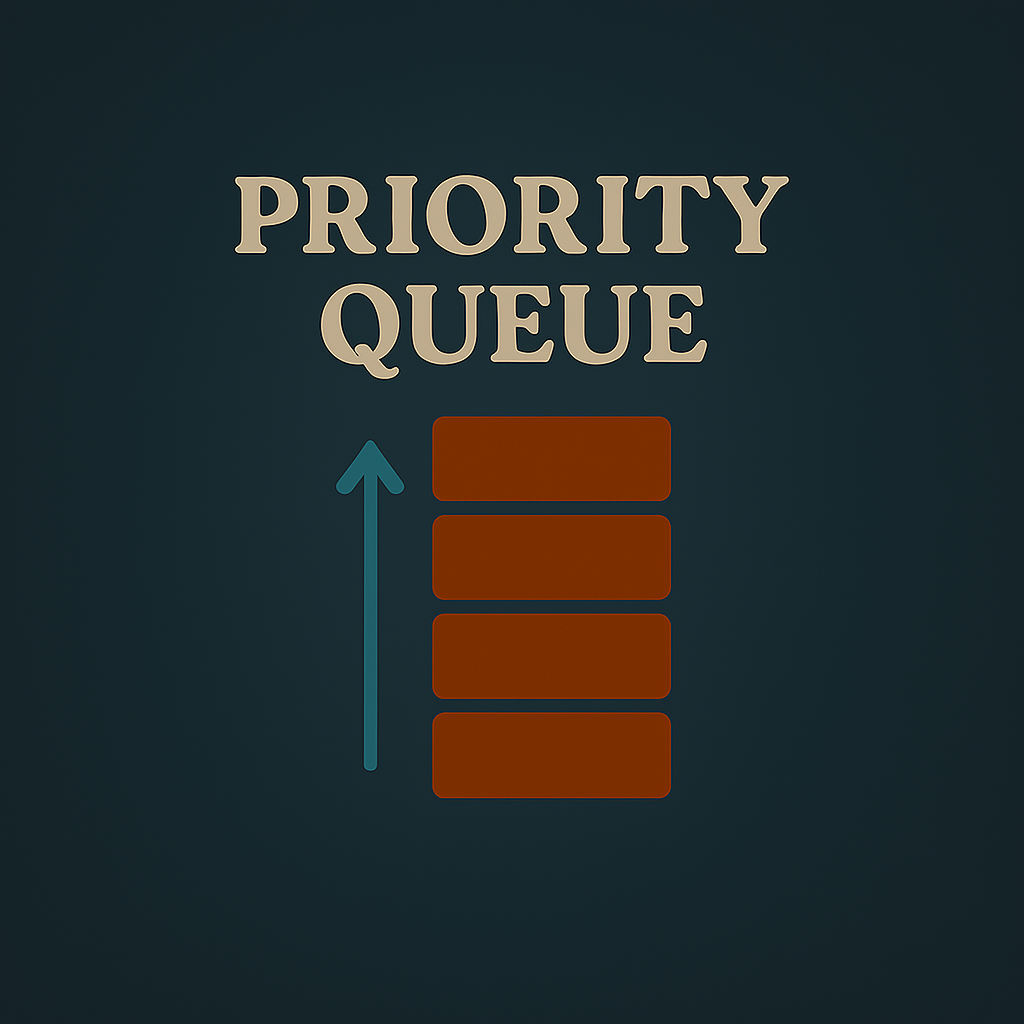
\includegraphics[height=13.88cm, width=17cm, keepaspectratio]{Pics/heap.png}
\end{center}

\chapter{Essential Heap Techniques }
\phantomsection                      % <-- creates a hyperlink anchor
\label{sec:heap}
\begin{itemize}
    \item \textbf{Heap Fundamentals:}
    \begin{itemize}
        \item Min-heap vs Max-heap:
        \begin{itemize}
            \item Min-heap: Root is smallest element (default in Python, Java)
            \item Max-heap: Root is largest element (implement with negative values)
        \end{itemize}
        \item Complexity:
        \begin{itemize}
            \item Insertion: $O(\log n)$
            \item Extraction: $O(\log n)$
            \item Peek: $O(1)$
            \item Heapify: $O(n)$
        \end{itemize}
        \item Implementation:
        \begin{itemize}
            \item Binary heap: Array representation with $i \rightarrow 2i+1, 2i+2$
            \item Language support: \texttt{heapq} (Python), \texttt{PriorityQueue} (Java), \texttt{priority\_queue} (C++)
        \end{itemize}
    \end{itemize}
    
    \item \textbf{Top-K Patterns:}
    \begin{itemize}
        \item Kth largest/smallest:
        \begin{itemize}
            \item Min-heap for Kth largest (keep heap size = k)
            \item Max-heap for Kth smallest
            \item Complexity: $O(n \log k)$ vs $O(n \log n)$ sorting
        \end{itemize}
        \item Top K frequent elements:
        \begin{itemize}
            \item Count frequencies + min-heap of size k
            \item Alternative: Bucket sort for $O(n)$ when frequencies bounded
        \end{itemize}
        \item K closest points:
        \begin{itemize}
            \item Max-heap based on distance (evict largest when size > k)
            \item Compare using squared distance to avoid sqrt
        \end{itemize}
    \end{itemize}
    
    \item \textbf{Stream Processing:}
    \begin{itemize}
        \item Median finder:
        \begin{itemize}
            \item Two heaps: Max-heap (left half), min-heap (right half)
            \item Balance: $|left| \leq |right| \leq |left| + 1$
            \item Median: Root of larger heap or average of roots
        \end{itemize}
        \item Sliding window median:
        \begin{itemize}
            \item Two heaps + lazy deletion hashmap
            \item Rebalance when heap tops are outside window
        \end{itemize}
    \end{itemize}
    
    \item \textbf{Scheduling \& Greedy:}
    \begin{itemize}
        \item Meeting rooms II:
        \begin{itemize}
            \item Min-heap of end times (track active meetings)
            \item Extract when $start \geq min(end)$
        \end{itemize}
        \item Task scheduler:
        \begin{itemize}
            \item Max-heap of frequencies + queue for cooldown
            \item Pattern: Execute highest frequency task, push to cooldown
        \end{itemize}
        \item Course schedule III:
        \begin{itemize}
            \item Max-heap of durations + greedy deadline management
            \item Replace longest task when new task can't fit
        \end{itemize}
    \end{itemize}
    
    \item \textbf{Pathfinding \& Graph Algorithms:}
    \begin{itemize}
        \item Dijkstra's algorithm:
        \begin{itemize}
            \item Min-heap of (distance, node)
            \item Decrease-key alternative: Multiple entries + visited set
        \end{itemize}
        \item Prim's MST:
        \begin{itemize}
            \item Min-heap of (edge-weight, node)
            \item Grow tree with cheapest edge
        \end{itemize}
        \item A* search:
        \begin{itemize}
            \item Min-heap of $f(n) = g(n) + h(n)$
            \item Heuristic must be admissible ($h(n) \leq$ actual cost)
        \end{itemize}
    \end{itemize}
    
    \item \textbf{Multiple Heap Techniques:}
    \begin{itemize}
        \item Min-max heap:
        \begin{itemize}
            \item Single DS supporting min and max in $O(1)$
            \item Alternative: Store two heaps with value mapping
        \end{itemize}
        \item K-way merge:
        \begin{itemize}
            \item Min-heap of (val, list-id, index)
            \item Extract min, push next from same list
        \end{itemize}
        \item Heap of heaps:
        \begin{itemize}
            \item Problems requiring partitioned heaps (e.g., multi-dimensional data)
        \end{itemize}
    \end{itemize}
    
    \item \textbf{Custom Heap Operations:}
    \begin{itemize}
        \item Heapify with custom comparator:
        \begin{itemize}
            \item Python: \texttt{heapq} with tuples \texttt{(priority, value)}
            \item C++: \texttt{priority\_queue<T, vector<T>, Compare>}
        \end{itemize}
        \item Decrease-key optimization:
        \begin{itemize}
            \item Without native support: Push duplicate entries + lazy deletion
            \item Track entry version for invalidation
        \end{itemize}
        \item Remove arbitrary element:
        \begin{itemize}
            \item Maintain auxiliary heap for deleted items
            \item Lazy cleanup when tops match
        \end{itemize}
    \end{itemize}
    
    \item \textbf{Edge Cases \& Pitfalls:}
    \begin{itemize}
        \item Empty heap: Check size before pop/top
        \item Duplicate values: Secondary comparator for stability
        \item Large heaps: Memory constraints with $O(n)$ space
        \item Floating points: Precision issues in distance calculations
        \item Stale entries: In lazy deletion schemes
        \item Concurrent access: Not thread-safe in most implementations
    \end{itemize}
    
    \item \textbf{Optimization Strategies:}
    \begin{itemize}
        \item Batch processing:
        \begin{itemize}
            \item Heapify entire collection instead of sequential inserts
            \item Reduces $O(n \log n)$ to $O(n)$
        \end{itemize}
        \item Size limitation:
        \begin{itemize}
            \item For top-k: Maintain heap size = k (save memory and time)
        \end{itemize}
        \item Precomputation:
        \begin{itemize}
            \item Compute distances/frequencies before heap operations
        \end{itemize}
    \end{itemize}
    
    \item \textbf{Hybrid Techniques:}
    \begin{itemize}
        \item Heap + Hashmap:
        \begin{itemize}
            \item LFU cache: Heap of (frequency, time, key) + key-value map
            \item Efficient updates with lazy deletion
        \end{itemize}
        \item Heap + Stack:
        \begin{itemize}
            \item Monotonic stack + heap for problems like largest rectangle
        \end{itemize}
        \item Heap + Union-Find:
        \begin{itemize}
            \item Kruskal's MST with heap for edges + UF for connectivity
        \end{itemize}
    \end{itemize}
    
    \item \textbf{Advanced Applications:}
    \begin{itemize}
        \item Huffman coding:
        \begin{itemize}
            \item Min-heap of frequencies, merge smallest two
        \end{itemize}
        \item External sorting:
        \begin{itemize}
            \item K-way merge of sorted chunks using heap
        \end{itemize}
        \item Skyline problem:
        \begin{itemize}
            \item Max-heap of heights with sweep line
            \item Remove heights when building exits view
        \end{itemize}
    \end{itemize}
    
    \item \textbf{Problem-Specific Patterns:}
    \begin{itemize}
        \item Kth largest in stream: Min-heap of size k
        \item Maximum performance team: Sort efficiency + min-heap for speed
        \item Reorganize string: Max-heap by frequency with cooldown
        \item Find median from data stream: Two-heap technique
        \label{itm:median}
        \item Minimum cost to connect sticks: Always merge smallest two
    \end{itemize}
    
    \item \textbf{Testing \& Debugging:}
    \begin{itemize}
        \item Validate heap properties: Parent $<$ children (min-heap)
        \item Check balance in two-heap structures
        \item Test with duplicate values
        \item Verify lazy deletion cleanup
        \item Small case verification: 0,1,2,3 elements
    \end{itemize}
    
    \item \textbf{Language-Specific Nuances:}
    \begin{itemize}
        \item Python:
        \begin{itemize}
            \item \texttt{heapq} is min-heap only
            \item Use \texttt{heapq.\_heapify\_max} for max-heap (limited operations)
        \end{itemize}
        \item Java:
        \begin{itemize}
            \item \texttt{PriorityQueue} min-heap default
            \item Max-heap: \texttt{new PriorityQueue<>(Collections.reverseOrder())}
        \end{itemize}
        \item C++:
        \begin{itemize}
            \item \texttt{priority\_queue<T>} is max-heap
            \item Min-heap: \texttt{priority\_queue<T, vector<T>, greater<T>>}
        \end{itemize}
    \end{itemize}
\end{itemize}
\section{Heap-Based DSA Problems Summary Table}
\begin{longtable}{|>{\raggedright\arraybackslash}p{3.2cm}|>{\columncolor{c2}\centering\arraybackslash}p{2.5cm}|>{\columncolor{c3}\raggedright\arraybackslash}p{4.3cm}|>{\columncolor{c4}\raggedright\arraybackslash}p{3.5cm}|>{\columncolor{c5}\color{white}\raggedright\arraybackslash}p{3.5cm}|}
\hline
\rowcolor{rclr}
\textbf{Problem Name} & \textbf{Time Complexity} & \textbf{Idea to Solve} & \textbf{Optimization Tip} & \textbf{Edge Cases} \\
\hline
\endfirsthead

\hline
\rowcolor{rclr}
\textbf{Problem Name} & \textbf{Time Complexity} & \textbf{Idea to Solve} & \textbf{Optimization Tip} & \textbf{Edge Cases} \\
\hline
\endhead
Heapify (min/max) & $\mathcal{O}(\log n)$ & Percolate down from given node to maintain heap property. & Start from last non-leaf node during build. & Node already satisfies heap \\
\hline
Build Heap & $\mathcal{O}(n)$ & Call heapify from last internal node to root. & Better than inserting one-by-one ($\mathcal{O}(n \log n)$). & Array already a heap \\
\hline
Insertion in Heap & $\mathcal{O}(\log n)$ & Insert at end, percolate up to fix violation. & Maintain array representation. & Duplicate or largest element \\
\hline
Decrease Key in Min Heap & $\mathcal{O}(\log n)$ & Update value and percolate up to restore heap. & Only decrease allowed in min-heap. & Key already smallest \\
\hline
Extract Min from Min Heap & $\mathcal{O}(\log n)$ & Replace root with last node, heapify down. & Efficient removal from top. & Heap has only one element \\
\hline
Heap Sort & $\mathcal{O}(n \log n)$ & Build max-heap, repeatedly extract max to end of array. & In-place, not stable. & Already sorted input \\
\hline
Sort K-Sorted Array & $\mathcal{O}(n \log k)$ & Use min-heap of size $k+1$ to get smallest available. & Maintain heap of current $k$ range. & k = 0 or very large \\
\hline
Buy Maximum Items with Given Sum & $\mathcal{O}(n + k \log n)$ & Sort or use min-heap, pick smallest until sum exhausted. & Use heap for faster access to smallest. & All items more than budget \\
\hline
K Largest Elements & $\mathcal{O}(n \log k)$ & Use min-heap of size k, keep top k largest. & Maintain heap of k elements. & k $>$ n \\
\hline
K Closest Elements & $\mathcal{O}(n \log k)$ & Use max-heap by distance from target. & Store elements as (diff, value). & Multiple same distance \\
\hline
Merge K Sorted Arrays (Similiar for K LL also) & $\mathcal{O}(n \log k)$ & Use min-heap to push smallest elements from each array. & Heap stores (value, array index, element index). & Varying lengths \\
\hline
Median of a Stream & $\mathcal{O}(\log n)$ & Use max-heap for left half and min-heap for right half. & Keep size difference $\leq 1$. & All elements same or increasing \\
\hline
\end{longtable}
\clearpage
\newgeometry{margin=1in}
% \documentclass[a4paper,10pt]{article}
% \usepackage[utf8]{inputenc}
% \usepackage{geometry}
% \usepackage[table]{xcolor}
% \usepackage{colortbl}
% \usepackage{color,soul}
% \geometry{margin=0.8in}
% \usepackage{xcolor}
% \usepackage{tikz}
% \usepackage{minted}
% \definecolor{bgcolor}{rgb}{0.8, 0.9, 0.5} % 
% \definecolor{bgcolor1}{rgb}{0.95, 0.95, 0.95} % Light Gray
% \definecolor{bgcolor2}{rgb}{0.85, 0.92, 1.0}  % Soft Blue
% \definecolor{bgcolor3}{rgb}{0.9, 0.85, 1.0}   % Light Purple
% \definecolor{bgcolor4}{rgb}{0.95, 0.88, 0.76} % Warm Beige
% \definecolor{bgcolor5}{rgb}{0.8, 0.95, 0.8}   % Gentle Green
% \definecolor{bgcolor6}{rgb}{1.0, 0.87, 0.87}  % Pastel Red
% \definecolor{bgcolor7}{rgb}{0.86, 0.93, 0.83} % Mint Green
% \definecolor{bgcolor8}{rgb}{0.98, 0.85, 0.94} % Soft Pink
% \definecolor{bgcolor9}{rgb}{0.87, 0.94, 0.98} % Sky Blue
% \definecolor{bgcolor10}{rgb}{0.96, 0.96, 0.82} % Pale Yellow
% 
% \begin{document}
% Heapify
\noindent\textbf{Problem: Heapify (min-heap)}
\begin{minted}[
bgcolor=bgcolor3,
frame=lines,
framesep=5mm,
rulecolor=\color{black},
linenos,
numbersep=5pt,
fontsize=\normalsize
]{python}
def min_heapify(arr, i, n):
    """
    Maintains min-heap property from index i downward.
    Time Complexity: O(log n), Space Complexity: O(1)
    """
    smallest = i
    left = 2 * i + 1
    right = 2 * i + 2
    
    if left < n and arr[left] < arr[smallest]:
        smallest = left
        
    if right < n and arr[right] < arr[smallest]:
        smallest = right
        
    if smallest != i:
        arr[i], arr[smallest] = arr[smallest], arr[i]
        min_heapify(arr, smallest, n)
\end{minted}

% Build Heap
\noindent\textbf{Problem: Build Heap}
\begin{minted}[
bgcolor=bgcolor7,
frame=lines,
framesep=5mm,
rulecolor=\color{black},
linenos,
numbersep=5pt,
fontsize=\normalsize
]{python}
def build_min_heap(arr):
    """
    Converts array into min-heap from bottom-up.
    Time Complexity: O(n), Space Complexity: O(1)
    """
    n = len(arr)
    for i in range(n // 2 - 1, -1, -1):
        min_heapify(arr, i, n)
\end{minted}

% Insertion in Heap
\noindent\textbf{Problem: Insertion in Heap}
\begin{minted}[
bgcolor=bgcolor5,
frame=lines,
framesep=5mm,
rulecolor=\color{black},
linenos,
numbersep=5pt,
fontsize=\normalsize
]{python}
def heap_insert(heap, value):
    """
    Inserts value into min-heap and maintains heap property.
    Time Complexity: O(log n), Space Complexity: O(1)
    """
    heap.append(value)
    i = len(heap) - 1
    # Bubble up
    while i > 0:
        parent = (i - 1) // 2
        if heap[parent] <= heap[i]:
            break
        heap[i], heap[parent] = heap[parent], heap[i]
        i = parent
\end{minted}

% Decrease Key in Min Heap
\noindent\textbf{Problem: Decrease Key in Min Heap}
\begin{minted}[
bgcolor=bgcolor8,
frame=lines,
framesep=5mm,
rulecolor=\color{black},
linenos,
numbersep=5pt,
fontsize=\normalsize
]{python}
def decrease_key(heap, i, new_val):
    """
    Decreases value at index i and maintains heap property.
    Time Complexity: O(log n), Space Complexity: O(1)
    """
    if new_val > heap[i]:
        raise ValueError("New value larger than current")
    
    heap[i] = new_val
    # Bubble up
    while i > 0:
        parent = (i - 1) // 2
        if heap[parent] <= heap[i]:
            break
        heap[i], heap[parent] = heap[parent], heap[i]
        i = parent
\end{minted}

% Extract Min from Min Heap
\noindent\textbf{Problem: Extract Min from Min Heap}
\begin{minted}[
bgcolor=bgcolor1,
frame=lines,
framesep=5mm,
rulecolor=\color{black},
linenos,
numbersep=5pt,
fontsize=\normalsize
]{python}
def extract_min(heap):
    """
    Extracts minimum element from min-heap.
    Time Complexity: O(log n), Space Complexity: O(1)
    """
    if not heap:
        return None
    
    min_val = heap[0]
    heap[0] = heap[-1]
    heap.pop()
    min_heapify(heap, 0, len(heap))
    return min_val
\end{minted}

% Heap Sort
\noindent\textbf{Problem: Heap Sort}
\begin{minted}[
bgcolor=bgcolor9,
frame=lines,
framesep=5mm,
rulecolor=\color{black},
linenos,
numbersep=5pt,
fontsize=\normalsize
]{python}
def heap_sort(arr):
    """
    Sorts array using heap sort algorithm.
    Time Complexity: O(n log n), Space Complexity: O(1)
    """
    n = len(arr)
    # Build max-heap (using min_heapify with sign flip)
    for i in range(n // 2 - 1, -1, -1):
        min_heapify(arr, i, n)
    
    # Extract elements one by one
    for i in range(n - 1, 0, -1):
        arr[0], arr[i] = arr[i], arr[0]
        min_heapify(arr, 0, i)
\end{minted}

% Sort K-Sorted Array
\noindent\textbf{Problem: Sort K-Sorted Array}
\begin{minted}[
bgcolor=bgcolor6,
frame=lines,
framesep=5mm,
rulecolor=\color{black},
linenos,
numbersep=5pt,
fontsize=\normalsize
]{python}
import heapq

def sort_k_sorted(arr, k):
    """
    Sorts array where each element is at most k positions away.
    Time Complexity: O(n log k), Space Complexity: O(k)
    """
    min_heap = []
    sorted_arr = []
    
    # Add first k+1 elements
    for i in range(min(k + 1, len(arr))):
        heapq.heappush(min_heap, arr[i])
    
    # Process remaining elements
    for i in range(k + 1, len(arr)):
        sorted_arr.append(heapq.heappop(min_heap))
        heapq.heappush(min_heap, arr[i])
    
    # Empty heap
    while min_heap:
        sorted_arr.append(heapq.heappop(min_heap))
    
    return sorted_arr
\end{minted}

% Buy Maximum Items
\noindent\textbf{Problem: Buy Maximum Items with Given Sum}
\begin{minted}[
bgcolor=bgcolor4,
frame=lines,
framesep=5mm,
rulecolor=\color{black},
linenos,
numbersep=5pt,
fontsize=\normalsize
]{python}
import heapq

def max_items(costs, budget):
    """
    Calculates maximum items that can be bought with given budget.
    Time Complexity: O(n log n), Space Complexity: O(1)
    """
    heapq.heapify(costs)
    count = 0
    
    while costs and budget >= costs[0]:
        budget -= heapq.heappop(costs)
        count += 1
    
    return count
\end{minted}

% K Largest Elements
\noindent\textbf{Problem: K Largest Elements}
\begin{minted}[
bgcolor=bgcolor10,
frame=lines,
framesep=5mm,
rulecolor=\color{black},
linenos,
numbersep=5pt,
fontsize=\normalsize
]{python}
import heapq

def k_largest(arr, k):
    """
    Finds k largest elements in array using min-heap.
    Time Complexity: O(n log k), Space Complexity: O(k)
    """
    min_heap = []
    for num in arr:
        heapq.heappush(min_heap, num)
        if len(min_heap) > k:
            heapq.heappop(min_heap)
    return min_heap
\end{minted}

% K Closest Elements
\noindent\textbf{Problem: K Closest Elements}
\begin{minted}[
bgcolor=bgcolor2,
frame=lines,
framesep=5mm,
rulecolor=\color{black},
linenos,
numbersep=5pt,
fontsize=\normalsize
]{python}
import heapq

def k_closest(points, k, origin=(0,0)):
    """
    Finds k closest points to origin using max-heap.
    Time Complexity: O(n log k), Space Complexity: O(k)
    """
    def distance(p):
        return (p[0]-origin[0])**2 + (p[1]-origin[1])**2
    
    max_heap = []
    for point in points:
        dist = -distance(point)  # Use negative for max-heap
        if len(max_heap) < k:
            heapq.heappush(max_heap, (dist, point))
        else:
            if dist > max_heap[0][0]:
                heapq.heapreplace(max_heap, (dist, point))
    
    return [point for (_, point) in max_heap]
\end{minted}

% Merge K Sorted Arrays
\noindent\textbf{Problem: Merge K Sorted Arrays}
\begin{minted}[
bgcolor=bgcolor7,
frame=lines,
framesep=5mm,
rulecolor=\color{black},
linenos,
numbersep=5pt,
fontsize=\normalsize
]{python}
import heapq

def merge_k_sorted(arrays):
    """
    Merges k sorted arrays into single sorted array.
    Time Complexity: O(n log k), Space Complexity: O(k)
    """
    min_heap = []
    result = []
    
    # Initialize heap with first element of each array
    for i, arr in enumerate(arrays):
        if arr:
            heapq.heappush(min_heap, (arr[0], i, 0))
    
    # Merge process
    while min_heap:
        val, arr_idx, idx = heapq.heappop(min_heap)
        result.append(val)
        if idx + 1 < len(arrays[arr_idx]):
            next_val = arrays[arr_idx][idx+1]
            heapq.heappush(min_heap, (next_val, arr_idx, idx+1))
    
    return result
\end{minted}

% Median of a Stream
\noindent\textbf{Problem: Median of a Stream}
\begin{minted}[
bgcolor=bgcolor5,
frame=lines,
framesep=5mm,
rulecolor=\color{black},
linenos,
numbersep=5pt,
fontsize=\normalsize
]{python}
import heapq

class MedianFinder:
    """
    Maintains median of streaming data using two heaps.
    Time Complexity: O(log n) per insertion, O(1) for median
    Space Complexity: O(n)
    """
    def __init__(self):
        self.small = []  # max-heap (store negative values)
        self.large = []  # min-heap

    def add_num(self, num: int) -> None:
        # Add to appropriate heap
        if not self.small or num <= -self.small[0]:
            heapq.heappush(self.small, -num)
        else:
            heapq.heappush(self.large, num)
        
        # Balance heaps
        if len(self.small) > len(self.large) + 1:
            heapq.heappush(self.large, -heapq.heappop(self.small))
        elif len(self.large) > len(self.small):
            heapq.heappush(self.small, -heapq.heappop(self.large))

    def find_median(self) -> float:
        if len(self.small) == len(self.large):
            return (-self.small[0] + self.large[0]) / 2
        return -self.small[0]
\end{minted}

% \end{document}

\newgeometry{margin=0.2in}
\vspace*{47mm}

\begin{center}

{\fontsize{55}{20}\selectfont \textcolor{headingcolor}{\bfseries GREEDY ALGO}}
\end{center}

\vspace{50mm}

\begin{center}

\includegraphics[height=13.88cm, width=17cm, keepaspectratio]{Pics/greedy.png}
\end{center}

\chapter{Essential Greedy Algorithm Techniques }
\phantomsection                      % <-- creates a hyperlink anchor
\label{sec:greedy}
\begin{itemize}
    \item \textbf{Core Greedy Principles:}
    \begin{itemize}
        \item Greedy choice property: Locally optimal choice leads to global optimum
        \item Optimal substructure: Solution to subproblems contributes to main solution
        \item Prove correctness: Use exchange argument or mathematical induction
    \end{itemize}
    
    \item \textbf{Interval Scheduling Patterns:}
    \begin{itemize}
        \item Activity selection:
        \begin{itemize}
            \item Sort by finish time, select earliest finishing
            \item Proof: Maximizes remaining time for more activities
        \end{itemize}
        \item Meeting rooms II:
        \begin{itemize}
            \item Track active meetings with min-heap (earliest end time)
            \item Complexity: $O(n \log n)$
        \end{itemize}
        \item Merge intervals:
        \begin{itemize}
            \item Sort by start time, merge overlapping intervals
            \item Edge: Adjacent intervals [1,3] and [3,5] → merge to [1,5]
        \end{itemize}
    \end{itemize}
    
    \item \textbf{Coin Change Variants:}
    \begin{itemize}
        \item Canonical systems: Greedy works (e.g., US coins: 1,5,10,25)
        \item Non-canonical systems: Requires DP (e.g., [1,3,4] for sum 6)
        \item Proof requirement: Must verify system is canonical
    \end{itemize}
    
    \item \textbf{Optimization Problems:}
    \begin{itemize}
        \item Fractional knapsack:
        \begin{itemize}
            \item Sort by value/weight ratio, take highest first
            \item Contrast: 0/1 knapsack requires DP
        \end{itemize}
        \item Job sequencing:
        \begin{itemize}
            \item Sort by profit, assign to latest possible slot
            \item Use disjoint-set for efficient slot finding
        \end{itemize}
        \item Huffman coding:
        \begin{itemize}
            \item Merge lowest frequency nodes with min-heap
            \item Complexity: $O(n \log n)$
        \end{itemize}
    \end{itemize}
    
    \item \textbf{Array Transformation Patterns:}
    \begin{itemize}
        \item Minimum increments:
        \begin{itemize}
            \item Make array strictly increasing: $arr[i] = \max(arr[i], arr[i-1]+1)$
            \item Total operations: $\sum \max(0, arr[i-1]+1 - arr[i])$
        \end{itemize}
        \item Gas station problems:
        \begin{itemize}
            \item Circular tour: Track deficit, reset when gas < 0
            \item Proof: If total gas $\geq$ total cost, solution exists
        \end{itemize}
    \end{itemize}
    
    \item \textbf{String Manipulation:}
    \begin{itemize}
        \item Lexicographical ordering:
        \begin{itemize}
            \item Remove k digits for smallest number: Use monotonic stack
            \item Edge: Leading zeros removal
        \end{itemize}
        \item Valid parentheses:
        \begin{itemize}
            \item Balance count: Increment for '(', decrement for ')'
            \item Greedy: Track current balance, fail if negative
        \end{itemize}
    \end{itemize}
    
    \item \textbf{Advanced Greedy Patterns:}
    \begin{itemize}
        \item K-way merging:
        \begin{itemize}
            \item Merge k sorted lists: Always pick smallest head using min-heap
            \item Extendible to external sorting
        \end{itemize}
        \item Egyptian fractions:
        \begin{itemize}
            \item Represent fraction as sum of unit fractions: $\frac{a}{b} = \frac{1}{\lceil b/a \rceil} + \cdots$
            \item Terminate when numerator becomes 1
        \end{itemize}
        \item Minimum spanning tree:
        \begin{itemize}
            \item Prim: Grow tree from vertex with min-heap
            \item Kruskal: Sort edges, add smallest that doesn't form cycle
        \end{itemize}
    \end{itemize}
    
    \item \textbf{Proof Techniques:}
    \begin{itemize}
        \item Greedy stays ahead: Show greedy is never worse than optimal
        \item Exchange argument: Transform optimal solution to greedy solution
        \item Mathematical induction: Base case and inductive step
        \item Counterexample search: Verify for small cases
    \end{itemize}
    
    \item \textbf{Edge Cases \& Pitfalls:}
    \begin{itemize}
        \item Empty input: Zero activities, empty array
        \item Single element: Trivial solutions
        \item Duplicate values: Stable sort to preserve order
        \item Negative values: Gas can be negative, values in knapsack
        \item Integer overflow: Large sums in operations count
        \item Ties in sorting: Secondary sort criteria matters
    \end{itemize}
    
    \item \textbf{Hybrid Approaches:}
    \begin{itemize}
        \item Greedy + Two pointers:
        \begin{itemize}
            \item Container with most water: Shorter line moves inward
        \end{itemize}
        \item Greedy + Binary search:
        \begin{itemize}
            \item Split array largest sum: Binary search on possible maximums
        \end{itemize}
        \item Greedy + DFS/BFS:
        \begin{itemize}
            \item Dijkstra: Greedy choice in priority queue
        \end{itemize}
    \end{itemize}
    
    \item \textbf{Common Problem Patterns:}
    \begin{itemize}
        \item Jump game I/II: Track maximum reachable index
        \item Candy distribution: Two-pass left-right then right-left
        \item Task scheduler: Schedule most frequent first with cooling
        \item Reorganize string: Place most frequent char first with heap
        \item Boats to save people: Sort and two pointers from ends
    \end{itemize}
    
    \item \textbf{Optimization Strategies:}
    \begin{itemize}
        \item Sorting optimization:
        \begin{itemize}
            \item Only sort necessary elements
            \item Use counting sort when possible
        \end{itemize}
        \item Early termination:
        \begin{itemize}
            \item Stop when solution becomes invalid
            \item Break when optimal solution found early
        \end{itemize}
        \item Space-time tradeoffs:
        \begin{itemize}
            \item Store additional state for O(1) decisions
            \item Precompute prefix/suffix arrays
        \end{itemize}
    \end{itemize}
    
    \item \textbf{When to Avoid Greedy:}
    \begin{itemize}
        \item When local optimum doesn't lead to global optimum
        \item When problem requires reconsidering earlier choices
        \item When constraints suggest DP $(n \leq 1000 \quad \text{vs} \quad n \leq 10^6)$

        \item When greedy choice isn't obvious or provable
    \end{itemize}
    
    \item \textbf{Testing \& Debugging:}
    \begin{itemize}
        \item Small test cases: Verify with hand-calculated results
        \item Property testing: Check invariants during execution
        \item Compare with brute force: For small n
        \item Corner cases: Max/min values, empty sets, duplicates
    \end{itemize}
\end{itemize}
\section{Greedy Algorithm-Based DSA Problems Summary Table}
\begin{longtable}{|>{\raggedright\arraybackslash}p{3.2cm}|>{\columncolor{c2}\centering\arraybackslash}p{2.5cm}|>{\columncolor{c3}\raggedright\arraybackslash}p{4.3cm}|>{\columncolor{c4}\raggedright\arraybackslash}p{3.5cm}|>{\columncolor{c5}\color{white}\raggedright\arraybackslash}p{3.5cm}|}
\hline
\rowcolor{rclr}
\textbf{Problem Name} & \textbf{Time Complexity} & \textbf{Idea to Solve} & \textbf{Optimization Tip} & \textbf{Edge Cases} \\
\hline
\endfirsthead

\hline
\textbf{Problem Name} & \textbf{Time Complexity} & \textbf{Idea to Solve} & \textbf{Optimization Tip} & \textbf{Edge Cases} \\
\hline
\endhead
Activity Selection Problem & $\mathcal{O}(n \log n)$ & Sort by finish time, select next non-overlapping activity. & Always pick earliest finishing activity. & All activities overlap or same finish time \\
\hline
Fractional Knapsack Problem & $\mathcal{O}(n \log n)$ & Sort items by value/weight ratio, take fraction if needed. & Use greedy for max value/unit weight. & All items too heavy or too light \\
\hline
Job Sequencing Problem & $\mathcal{O}(n \log n + n d)$ & Sort jobs by profit, assign to latest free slot before deadline. & Use disjoint set/array for free slot finding. & Jobs with same deadlines or 0 deadline \\
\hline
Huffman Coding & $\mathcal{O}(n \log n)$ & Build min-heap of frequencies, combine lowest two recursively. & Use priority queue for optimal code tree. & All frequencies same or 1 symbol only \\
\hline
\end{longtable}
\clearpage
\newgeometry{margin=1in}
% \documentclass[a4paper,10pt]{article}
% \usepackage[utf8]{inputenc}
% \usepackage{geometry}
% \usepackage[table]{xcolor}
% \usepackage{colortbl}
% \usepackage{color,soul}
% \geometry{margin=0.8in}
% \usepackage{xcolor}
% \usepackage{tikz}
% \usepackage{minted}
% \definecolor{bgcolor}{rgb}{0.8, 0.9, 0.5} % 
% \definecolor{bgcolor1}{rgb}{0.95, 0.95, 0.95} % Light Gray
% \definecolor{bgcolor2}{rgb}{0.85, 0.92, 1.0}  % Soft Blue
% \definecolor{bgcolor3}{rgb}{0.9, 0.85, 1.0}   % Light Purple
% \definecolor{bgcolor4}{rgb}{0.95, 0.88, 0.76} % Warm Beige
% \definecolor{bgcolor5}{rgb}{0.8, 0.95, 0.8}   % Gentle Green
% \definecolor{bgcolor6}{rgb}{1.0, 0.87, 0.87}  % Pastel Red
% \definecolor{bgcolor7}{rgb}{0.86, 0.93, 0.83} % Mint Green
% \definecolor{bgcolor8}{rgb}{0.98, 0.85, 0.94} % Soft Pink
% \definecolor{bgcolor9}{rgb}{0.87, 0.94, 0.98} % Sky Blue
% \definecolor{bgcolor10}{rgb}{0.96, 0.96, 0.82} % Pale Yellow
% 
% \begin{document}
% Activity Selection Problem
\noindent\textbf{Problem: Activity Selection Problem}
\begin{minted}[
bgcolor=bgcolor3,
frame=lines,
framesep=5mm,
rulecolor=\color{black},
linenos,
numbersep=5pt,
fontsize=\normalsize
]{python}
def activity_selection(start, finish):
    """
    Selects maximum number of non-overlapping activities.
    Time Complexity: O(n log n), Space Complexity: O(n)
    """
    # Sort activities by finish time
    activities = sorted(zip(start, finish), key=lambda x: x[1])
    count = 1
    last_finish = activities[0][1]
    
    # Select activities
    for i in range(1, len(activities)):
        s, f = activities[i]
        if s >= last_finish:
            count += 1
            last_finish = f
    
    return count
\end{minted}

% Fractional Knapsack Problem
\noindent\textbf{Problem: Fractional Knapsack Problem}
\begin{minted}[
bgcolor=bgcolor7,
frame=lines,
framesep=5mm,
rulecolor=\color{black},
linenos,
numbersep=5pt,
fontsize=\normalsize
]{python}
def fractional_knapsack(weights, values, capacity):
    """
    Maximizes value in knapsack using fractional items.
    Time Complexity: O(n log n), Space Complexity: O(n)
    """
    # Calculate value per unit weight
    items = [(v/w, w, v) for w, v in zip(weights, values)]
    items.sort(reverse=True)  # Sort by value/weight descending
    
    total_value = 0.0
    for ratio, weight, value in items:
        if capacity >= weight:
            # Take whole item
            total_value += value
            capacity -= weight
        else:
            # Take fraction
            total_value += ratio * capacity
            break
    
    return total_value
\end{minted}

% Job Sequencing Problem
\noindent\textbf{Problem: Job Sequencing Problem}
\begin{minted}[
bgcolor=bgcolor5,
frame=lines,
framesep=5mm,
rulecolor=\color{black},
linenos,
numbersep=5pt,
fontsize=\normalsize
]{python}
def job_sequencing(jobs):
    """
    Maximizes profit by scheduling jobs within deadlines.
    Time Complexity: O(n²), Space Complexity: O(n)
    """
    # Sort jobs by profit descending
    jobs.sort(key=lambda x: x[2], reverse=True)
    
    # Find maximum deadline
    max_deadline = max(job[1] for job in jobs)
    
    # Initialize result array
    result = [None] * (max_deadline + 1)
    total_profit = 0
    
    for job in jobs:
        # Find latest available slot before deadline
        for j in range(job[1], 0, -1):
            if j <= max_deadline and result[j] is None:
                result[j] = job[0]  # Job ID
                total_profit += job[2]  # Profit
                break
    
    # Return sequence and profit
    sequence = [job_id for job_id in result if job_id is not None]
    return sequence, total_profit
\end{minted}

% Huffman Coding
\noindent\textbf{Problem: Huffman Coding}
\begin{minted}[
bgcolor=bgcolor8,
frame=lines,
framesep=5mm,
rulecolor=\color{black},
linenos,
numbersep=5pt,
fontsize=\normalsize
]{python}
import heapq
from collections import defaultdict

class Node:
    def __init__(self, char=None, freq=0):
        self.char = char
        self.freq = freq
        self.left = None
        self.right = None
        
    # For heap comparison
    def __lt__(self, other):
        return self.freq < other.freq

def build_huffman_tree(text):
    """
    Builds Huffman tree from character frequencies.
    Time Complexity: O(n log n), Space Complexity: O(n)
    """
    # Count character frequencies
    freq = defaultdict(int)
    for char in text:
        freq[char] += 1
    
    # Create leaf nodes and push to min-heap
    min_heap = []
    for char, count in freq.items():
        heapq.heappush(min_heap, Node(char, count))
    
    # Build Huffman tree
    while len(min_heap) > 1:
        left = heapq.heappop(min_heap)
        right = heapq.heappop(min_heap)
        
        merged = Node(freq=left.freq + right.freq)
        merged.left = left
        merged.right = right
        heapq.heappush(min_heap, merged)
    
    return heapq.heappop(min_heap)

def generate_codes(root, prefix="", code_map=None):
    """
    Generates Huffman codes from tree traversal.
    Time Complexity: O(n), Space Complexity: O(n)
    """
    if code_map is None:
        code_map = {}
    
    if root.char is not None:
        code_map[root.char] = prefix
    else:
        generate_codes(root.left, prefix + "0", code_map)
        generate_codes(root.right, prefix + "1", code_map)
    
    return code_map

def huffman_encode(text):
    """
    Encodes text using Huffman coding.
    Returns encoded text and code mapping.
    """
    if not text:
        return "", {}
    
    root = build_huffman_tree(text)
    codes = generate_codes(root)
    encoded = "".join(codes[char] for char in text)
    return encoded, codes
\end{minted}

% \end{document}

\newgeometry{margin=0.2in}
\vspace*{47mm}

\begin{center}

{\fontsize{55}{20}\selectfont \textcolor{headingcolor}{\bfseries RECURSION}}
\end{center}

\vspace{50mm}

\begin{center}

\includegraphics[height=13.88cm, width=17cm, keepaspectratio]{Pics/recursion.png}
\end{center}

\chapter{Essential Techniques for Recursion }
\phantomsection                      % <-- creates a hyperlink anchor
\label{sec:recursion}
\begin{itemize}[leftmargin=*]
    \item \textbf{Core Concepts:}
    \begin{itemize}
        \item Base Case: The stopping condition that prevents infinite recursion
        \item Recursive Case: The part where function calls itself with modified parameters
        \item State Reduction: Each recursive call should move closer to base case
        \item Trust the Process: Assume recursive calls work correctly for smaller inputs
        \item Call Stack: Understanding how function calls are stored and managed
    \end{itemize}

    \item \textbf{Recursion Design Process:}
    \begin{itemize}
        \item Step 1: Identify the smallest possible input (base case)
        \item Step 2: Define what the function should return for base case
        \item Step 3: Assume function works for smaller inputs
        \item Step 4: Use smaller solutions to build current solution
        \item Step 5: Ensure each call moves toward base case
        \item Step 6: Verify termination condition is always reachable
    \end{itemize}
\end{itemize}

\begin{itemize}[leftmargin=*]
    \item \textbf{Linear Recursion:}
    \begin{itemize}
        \item Factorial Pattern: $f(n) = n \times f(n-1)$ with $f(0)=1$
        \item Fibonacci Pattern: $f(n)=f(n-1)+f(n-2)$ with base cases
        \item Sum Pattern: $sum(n)=n + sum(n-1)$ for arithmetic operations
        \item Countdown Pattern: Process element, recurse on remaining elements
        \item Build-up Pattern: Recurse first, then process current element
    \end{itemize}

    \item \textbf{Tree Recursion:}
    \begin{itemize}
        \item Binary Tree Traversal: Process root, recurse on left and right subtrees
        \item Path Sum Problems: Check if path exists with given sum
        \item Tree Height/Depth: $height=1+\max(leftHeight,\,rightHeight)$
        \item Diameter Problems: Maximum path length through any node
        \item Symmetric Tree: Check if tree is mirror of itself
    \end{itemize}

    \item \textbf{Divide and Conquer:}
    \begin{itemize}
        \item Merge Sort Pattern: Divide array, sort halves, merge results
        \item Quick Sort Pattern: Choose pivot, partition, recurse on subarrays
        \item Binary Search Pattern: Compare with middle, recurse on appropriate half
        \item Maximum Subarray: Divide array, find max in left, right, and crossing
        \item Closest Pair: Divide points, find closest in each half and across
    \end{itemize}
\end{itemize}

\begin{itemize}[leftmargin=*]
    \item \textbf{Backtracking:}
    \begin{itemize}
        \item Template Pattern: Choose → Explore → Unchoose (backtrack)
        \item Permutation Generation: Generate all arrangements of elements
        \item Combination Generation: Generate all subsets of given size
        \item N-Queens Problem: Place queens without attacking each other
        \item Sudoku Solver: Fill grid following Sudoku rules
        \item Maze Solving: Find path through maze using backtracking
        \item Graph Coloring: Assign colors to vertices without conflicts
    \end{itemize}

    \item \textbf{Memoization (Top-Down DP):}
    \begin{itemize}
        \item Overlapping Subproblems: Same inputs computed multiple times
        \item Cache Results: Store computed results to avoid recomputation
        \item Hash Map Cache: Use map/dictionary for flexible parameter caching
        \item Array Cache: Use arrays when parameters have fixed bounds
        \item Multi-dimensional Cache: For functions with multiple parameters
        \item Cache Key Design: How to map function parameters to cache keys
    \end{itemize}

    \item \textbf{Tail Recursion:}
    \begin{itemize}
        \item Tail Call Optimization: When recursive call is the last operation
        \item Accumulator Pattern: Pass accumulated result as parameter
        \item Iterative Conversion: Convert tail recursion to iteration
        \item Stack Space Optimization: Reduce stack usage through tail calls
        \item Continuation Passing: Alternative approach to tail recursion
    \end{itemize}
\end{itemize}

\begin{itemize}[leftmargin=*]
    \item \textbf{Array/List Recursion:}
    \begin{itemize}
        \item Head-Tail Pattern: Process first element, recurse on rest
        \item Two-Pointer Recursion: Recursively process from both ends
        \item Subarray Problems: Recurse on different subarrays
        \item Reverse Array: Swap elements recursively from ends
        \item Array Search: Binary search and linear search variations
        \item Merge Operations: Combine sorted arrays recursively
    \end{itemize}

    \item \textbf{String Recursion:}
    \begin{itemize}
        \item Palindrome Check: Compare first and last characters recursively
        \item String Reversal: Build reversed string character by character
        \item Substring Generation: Generate all possible substrings
        \item Pattern Matching: Recursive string matching algorithms
        \item Edit Distance: Minimum operations to transform strings
        \item Longest Common Subsequence: Find common subsequence recursively
    \end{itemize}

    \item \textbf{Tree and Graph Recursion:}
    \begin{itemize}
        \item DFS Implementation: Recursive depth-first search
        \item Path Finding: Find paths between nodes recursively
        \item Tree Construction: Build trees from traversal sequences
        \item Subtree Problems: Solve problems within subtrees
        \item Graph Cycle Detection: Detect cycles using recursive DFS
        \item Topological Sort: Recursive implementation using DFS
    \end{itemize}
\end{itemize}

\begin{itemize}[leftmargin=*]
    \item \textbf{Number Theory:}
    \begin{itemize}
        \item GCD/LCM: Euclidean algorithm using recursion
        \item Modular Exponentiation: $a^b \bmod m$ using fast exponentiation
        \item Prime Factorization: Recursive factorization algorithms
        \item Catalan Numbers: Recursive computation with applications
        \item Pascal's Triangle: Binomial coefficients using recursion
    \end{itemize}

    \item \textbf{Combinatorics:}
    \begin{itemize}
        \item Permutation Count: $P(n,r)=n\times P(n-1,r-1)$
        \item Combination Count: $C(n,r)=C(n-1,r-1)+C(n-1,r)$
        \item Subset Generation: Generate all $2^n$ subsets
        \item Partition Problems: Ways to partition numbers or sets
        \item Stirling Numbers: Recursive computation for set partitions
    \end{itemize}

    \item \textbf{Geometry:}
    \begin{itemize}
        \item Fractal Generation: Recursive geometric patterns
        \item Convex Hull: Divide and conquer approach
        \item Closest Pair: Recursive solution for closest point pair
        \item Area Calculation: Recursive polygon area computation
        \item Tree Structures: Recursive geometric tree problems
    \end{itemize}
\end{itemize}

\begin{itemize}[leftmargin=*]
    \item \textbf{Avoiding Stack Overflow:}
    \begin{itemize}
        \item Iterative Conversion: Convert recursion to iteration when possible
        \item Tail Recursion: Use tail calls to reduce stack usage
        \item Explicit Stack: Simulate recursion using explicit stack
        \item Increase Stack Limit: Platform-specific stack size increases
        \item Divide Problem Size: Reduce recursion depth by different partitioning
    \end{itemize}

    \item \textbf{Performance Optimization:}
    \begin{itemize}
        \item Memoization: Cache results to avoid redundant calculations
        \item Early Termination: Return immediately when answer is found
        \item Pruning: Skip branches that can't lead to optimal solution
        \item Parameter Optimization: Minimize number of parameters passed
        \item Reference Passing: Avoid copying large data structures
    \end{itemize}
\end{itemize}

\begin{itemize}[leftmargin=*]
    \item \textbf{When to Use Recursion:}
    \begin{itemize}
        \item Self-Similar Structure: Problem has similar subproblems
        \item Tree/Graph Problems: Natural recursive structure
        \item Divide and Conquer: Problem can be divided into similar subproblems
        \item Backtracking Needed: Need to explore all possibilities
        \item Mathematical Induction: Problem follows inductive structure
        \item Nested Structures: Data has recursive nesting
    \end{itemize}

    \item \textbf{When NOT to Use Recursion:}
    \begin{itemize}
        \item Simple Iteration: Linear problems better solved iteratively
        \item Stack Overflow Risk: Very deep recursion with large inputs
        \item No Overlapping Subproblems: Pure recursion without memoization inefficient
        \item Tail Recursion: Often better converted to iteration
        \item Memory Constraints: Limited stack space available
    \end{itemize}
\end{itemize}
\begin{itemize}[leftmargin=*]
    \item \textbf{Search Problems:}
    \begin{itemize}
        \item Binary Search: Recursive elimination of half search space
        \item Depth-First Search: Recursive graph/tree exploration
        \item Backtracking Search: Explore all paths with backtracking
        \item Branch and Bound: Recursive optimization with pruning
        \item Game Trees: Minimax algorithm for two-player games
    \end{itemize}

    \item \textbf{Generation Problems:}
    \begin{itemize}
        \item Permutation Generation: All arrangements of elements
        \item Combination Generation: All selections of elements
        \item Subset Generation: All possible subsets
        \item Parentheses Generation: All valid parentheses combinations
        \item Path Generation: All paths between points
    \end{itemize}

    \item \textbf{Optimization Problems:}
    \begin{itemize}
        \item Knapsack Problem: Recursive choice—include or exclude item
        \item Coin Change: Minimum coins for amount using recursion
        \item Edit Distance: Minimum operations to transform strings
        \item Longest Increasing Subsequence: Recursive DP approach
        \item Matrix Chain Multiplication: Optimal parenthesization
    \end{itemize}
\end{itemize}

\begin{itemize}[leftmargin=*]
    \item \textbf{Parameter Design:}
    \begin{itemize}
        \item Minimal Parameters: Pass only necessary information
        \item Index Parameters: Use indices instead of creating subarrays
        \item Accumulator Parameters: Build result as parameter
        \item State Parameters: Track current state of computation
        \item Boundary Parameters: Pass start/end indices for ranges
    \end{itemize}

    \item \textbf{Return Value Strategies:}
    \begin{itemize}
        \item Direct Return: Return computed value directly
        \item Boolean Return: Return success/failure status
        \item Multiple Returns: Return multiple values using pairs/tuples
        \item Reference Parameters: Modify parameters instead of returning
        \item Global Variables: Use global state for complex returns
    \end{itemize}

    \item \textbf{Base Case Design:}
    \begin{itemize}
        \item Empty Input: Handle empty arrays, strings, trees
        \item Single Element: Handle single element cases
        \item Boundary Values: Handle minimum/maximum input values
        \item Invalid Input: Handle invalid or edge case inputs
        \item Multiple Base Cases: Some problems need several base cases
    \end{itemize}
\end{itemize}

\begin{itemize}[leftmargin=*]
    \item \textbf{Common Mistakes:}
    \begin{itemize}
        \item Missing Base Case: Recursion never terminates
        \item Wrong Base Case: Incorrect return value for base case
        \item Infinite Recursion: Parameters don't move toward base case
        \item Stack Overflow: Recursion too deep for available stack
        \item Parameter Errors: Incorrect parameter passing in recursive calls
    \end{itemize}

    \item \textbf{Debugging Techniques:}
    \begin{itemize}
        \item Trace Execution: Manually trace through small examples
        \item Print Statements: Add debug prints to track recursive calls
        \item Call Stack Visualization: Draw call stack for understanding
        \item Base Case Testing: Test base cases independently
        \item Parameter Validation: Verify parameters are changing correctly
    \end{itemize}
\end{itemize}

\begin{itemize}[leftmargin=*]
    \item \textbf{Quick Implementation:}
    \begin{itemize}
        \item Template Patterns: Memorize common recursive templates
        \item Standard Algorithms: Know recursive implementations of standard algorithms
        \item Memoization Template: Have ready template for memoized recursion
        \item Backtracking Template: Standard backtracking structure
        \item Tree Traversal: Quick implementations of tree algorithms
    \end{itemize}

    \item \textbf{Problem Analysis:}
    \begin{itemize}
        \item Constraint Analysis: Check if recursion depth will be manageable
        \item Time Complexity: Analyze recursive time complexity using recurrence relations
        \item Space Complexity: Consider call stack space in addition to explicit space
        \item Subproblem Identification: Look for overlapping subproblems
        \item Pattern Matching: Recognize which recursive pattern applies
    \end{itemize}
\end{itemize}

\begin{itemize}[leftmargin=*]
    \item \textbf{Mutual Recursion:}
    \begin{itemize}
        \item Even-Odd Functions: Functions that call each other alternately
        \item State Machine: Recursive implementation of state machines
        \item Grammar Parsing: Recursive descent parsers
        \item Game Theory: Player alternation in game tree search
        \item Protocol Implementation: Network protocol state handling
    \end{itemize}

    \item \textbf{Higher-Order Recursion:}
    \begin{itemize}
        \item Functions as Parameters: Pass functions to recursive functions
        \item Currying: Transform multi-parameter recursion
        \item Continuation Passing: Advanced control flow techniques
        \item Lazy Evaluation: Delay computation in recursive structures
        \item Functional Programming: Pure functional recursive approaches
    \end{itemize}

    \item \textbf{Mathematical Analysis:}
    \begin{itemize}
        \item Recurrence Relations: $T(n)=aT(n/b)+f(n)$
        \item Master Theorem: Analyze divide-and-conquer recurrences
        \item Generating Functions: Convert recursions to algebraic form
        \item Asymptotic Analysis: Big-O analysis of recursive algorithms
        \item Recursion Trees: Visual method for analyzing complexity
    \end{itemize}
\end{itemize}

\begin{itemize}[leftmargin=*]
    \item \textbf{C++ Recursion:}
    \begin{itemize}
        \item Stack Size: Default stack size limitations
        \item Inline Functions: Compiler optimizations for simple recursions
        \item Template Recursion: Compile-time recursive computations
        \item Exception Handling: Stack unwinding in recursive functions
        \item Memory Management: Automatic vs manual memory management
    \end{itemize}

    \item \textbf{Python Recursion:}
    \begin{itemize}
        \item Recursion Limit: \texttt{sys.setrecursionlimit()} for deep recursion
        \item Function Decorators: \texttt{@lru\_cache} for automatic memoization
        \item Generator Functions: \texttt{yield} for memory-efficient recursion
        \item Tail Call: Python doesn't optimize tail calls
        \item Exception Handling: \texttt{RecursionError} for stack overflow
    \end{itemize}
\end{itemize}
\section{Recursion-Based DSA Problems Summary Table}
\begin{longtable}{|>{\raggedright\arraybackslash}p{3.2cm}|>{\columncolor{c2}\centering\arraybackslash}p{2.5cm}|>{\columncolor{c3}\raggedright\arraybackslash}p{4.3cm}|>{\columncolor{c4}\raggedright\arraybackslash}p{3.5cm}|>{\columncolor{c5}\color{white}\raggedright\arraybackslash}p{3.5cm}|}
\hline
\rowcolor{rclr}
\textbf{Problem Name} & \textbf{Time Complexity} & \textbf{Idea to Solve} & \textbf{Optimization Tip} & \textbf{Edge Cases} \\
\hline
\endfirsthead
\hline
\textbf{Problem Name} & \textbf{Time Complexity} & \textbf{Idea to Solve} & \textbf{Optimization Tip} & \textbf{Edge Cases} \\
\hline
\endhead
Palindrome Check (Recursion) & $\mathcal{O}(n)$ & Check first and last chars, recurse on substring. & Use 2-pointer recursive technique. & Empty or single char string \\
\hline
Count Set Bits from 1 to N & $\mathcal{O}(\log N)$ & Recursively count set bits using patterns in binary. & Use most significant bit position. & N = 0 or power of 2 \\
\hline
Rope Cutting Problem & $\mathcal{O}(3^n)$ & Try all 3 cuts recursively, take max of all valid. & Use memoization to avoid recomputation. & Cut lengths not possible \\
\hline
Generate Subsets & $\mathcal{O}(2^n)$ & For each element, include or exclude recursively. & Use backtracking to store current subset. & Empty set, duplicate elements \\
\hline
No. of Subsets with Given Sum (Recursive) & $\mathcal{O}(2^n)$  & Try including/excluding current element recursively. & Use DP or memoization. & Negative numbers, sum = 0 \\
\hline
Tower of Hanoi & $\mathcal{O}(2^n)$ & Move n-1 disks to aux, nth to target, then n-1 to target. & Direct formula: $2^n - 1$ moves. & n = 1, source = destination \\
\hline
Josephus Problem & $\mathcal{O}(n)$ & Use recursive relation $J(n, k) = (J(n-1, k) + k) \% n$. & Convert to 0-based index for clean recursion. & k = 1, n = 1 \\
\hline
Printing All Permutations & $\mathcal{O}(n!)$ & Swap elements recursively and backtrack. & Use visited[] or backtracking for non-repetition. & Duplicate elements \\
\hline
Permutations with Duplicates & $O(n!)$ & Sort input, use visited[] and skip same element at same level & Backtracking with used set check & All elements same \\
\hline
\end{longtable}
\clearpage
\newgeometry{margin=1in}
% \documentclass[a4paper,10pt]{article}
% \usepackage[utf8]{inputenc}
% \usepackage{geometry}
% \usepackage[table]{xcolor}
% \usepackage{colortbl}
% \usepackage{color,soul}
% \geometry{margin=0.8in}
% \usepackage{xcolor}
% \usepackage{tikz}
% \usepackage{minted}
% \definecolor{bgcolor}{rgb}{0.8, 0.9, 0.5} % 
% \definecolor{bgcolor1}{rgb}{0.95, 0.95, 0.95} % Light Gray
% \definecolor{bgcolor2}{rgb}{0.85, 0.92, 1.0}  % Soft Blue
% \definecolor{bgcolor3}{rgb}{0.9, 0.85, 1.0}   % Light Purple
% \definecolor{bgcolor4}{rgb}{0.95, 0.88, 0.76} % Warm Beige
% \definecolor{bgcolor5}{rgb}{0.8, 0.95, 0.8}   % Gentle Green
% \definecolor{bgcolor6}{rgb}{1.0, 0.87, 0.87}  % Pastel Red
% \definecolor{bgcolor7}{rgb}{0.86, 0.93, 0.83} % Mint Green
% \definecolor{bgcolor8}{rgb}{0.98, 0.85, 0.94} % Soft Pink
% \definecolor{bgcolor9}{rgb}{0.87, 0.94, 0.98} % Sky Blue
% \definecolor{bgcolor10}{rgb}{0.96, 0.96, 0.82} % Pale Yellow
% 
% \begin{document}
% Palindrome Check (Recursion)
\noindent\textbf{Problem: Palindrome Check (Recursion)}
\begin{minted}[
bgcolor=bgcolor3,
frame=lines,
framesep=5mm,
rulecolor=\color{black},
linenos,
numbersep=5pt,
fontsize=\normalsize
]{python}
def is_palindrome(s: str, start: int, end: int) -> bool:
    """
    Checks if substring s[start:end+1] is palindrome using recursion.
    Time Complexity: O(n), Space Complexity: O(n) for recursion stack.
    """
    if start >= end:
        return True
    if s[start] != s[end]:
        return False
    return is_palindrome(s, start+1, end-1)
\end{minted}

% Count Set Bits from 1 to N
\noindent\textbf{Problem: Count Set Bits from 1 to N}
\begin{minted}[
bgcolor=bgcolor7,
frame=lines,
framesep=5mm,
rulecolor=\color{black},
linenos,
numbersep=5pt,
fontsize=\normalsize
]{python}
def count_set_bits(n: int) -> int:
    """
    Counts total set bits in all numbers from 1 to n using bit patterns.
    Time Complexity: O(log n), Space Complexity: O(1)
    """
    if n <= 0:
        return 0
        
    # Find highest power of 2 <= n
    x = 0
    while (1 << x) <= n:
        x += 1
    x -= 1
    
    # Calculate total set bits
    bits_till_2x = x * (1 << (x-1))
    msb_after_2x = n - (1 << x) + 1
    rest = n - (1 << x)
    return bits_till_2x + msb_after_2x + count_set_bits(rest)
\end{minted}

% Rope Cutting Problem
\noindent\textbf{Problem: Rope Cutting Problem}
\begin{minted}[
bgcolor=bgcolor5,
frame=lines,
framesep=5mm,
rulecolor=\color{black},
linenos,
numbersep=5pt,
fontsize=\normalsize
]{python}
def max_rope_cuts(n: int, a: int, b: int, c: int) -> int:
    """
    Maximizes number of rope cuts of lengths a, b, c from rope of length n.
    Time Complexity: O(3^n), Space Complexity: O(n) for recursion stack.
    """
    if n == 0:
        return 0
    if n < 0:
        return -1
        
    res = max(
        max_rope_cuts(n-a, a, b, c),
        max_rope_cuts(n-b, a, b, c),
        max_rope_cuts(n-c, a, b, c)
    )
    
    return res + 1 if res >= 0 else -1
\end{minted}

% Generate Subsets
\noindent\textbf{Problem: Generate Subsets}
\begin{minted}[
bgcolor=bgcolor8,
frame=lines,
framesep=5mm,
rulecolor=\color{black},
linenos,
numbersep=5pt,
fontsize=\normalsize
]{python}
def generate_subsets(nums: List[int]) -> List[List[int]]:
    """
    Generates all subsets of given list using recursion.
    Time Complexity: O(2^n), Space Complexity: O(n) for recursion stack.
    """
    def backtrack(start, path):
        result.append(path[:])
        #   For each choice of next element…
        for i in range(start, len(nums)):
            #    a) INCLUDE nums[i]
            path.append(nums[i])
            backtrack(i+1, path)
            #    b) EXCLUDE nums[i] (undo include)
            path.pop()
    ##############################ALTERNATE###########################
    def backtrack(idx, path):
        if idx == len(nums):
            result.append(path[:])
            return
        # exclude nums[idx]
        helper(idx+1, path)
        # include nums[idx]
        path.append(nums[idx])
        helper(idx+1, path)
        path.pop()

            
    result = []
    backtrack(0, [])
    return result
\end{minted}

% Subset Sum (Recursive)
\noindent\textbf{Problem: Number of Subsets with Given Sum (Recursive)}
\begin{minted}[
bgcolor=bgcolor1,
frame=lines,
framesep=5mm,
rulecolor=\color{black},
linenos,
numbersep=5pt,
fontsize=\normalsize
]{python}
def subset_sum_count(nums: List[int], target: int) -> int:
    """
    Counts number of subsets that sum to target (recursive).
    Time Complexity: O(2^n), Space Complexity: O(n) for recursion stack.
    """
    def helper(i, current_sum):
        if current_sum == target:
            return 1
        if i == len(nums) or current_sum > target:
            return 0
        return helper(i+1, current_sum + nums[i]) + helper(i+1, current_sum)
        
    return helper(0, 0)
\end{minted}

% Tower of Hanoi
\noindent\textbf{Problem: Tower of Hanoi}
\begin{minted}[
bgcolor=bgcolor9,
frame=lines,
framesep=5mm,
rulecolor=\color{black},
linenos,
numbersep=5pt,
fontsize=\normalsize
]{python}
def tower_of_hanoi(n: int, source: str, auxiliary: str, destination: str) -> None:
    """
    Prints steps to solve Tower of Hanoi problem.
    Time Complexity: O(2^n), Space Complexity: O(n) for recursion stack.
    """
    if n == 1:
        print(f"Move disk 1 from {source} to {destination}")
        return
    tower_of_hanoi(n-1, source, destination, auxiliary)
    print(f"Move disk {n} from {source} to {destination}")
    tower_of_hanoi(n-1, auxiliary, source, destination)
\end{minted}

% Josephus Problem
\noindent\textbf{Problem: Josephus Problem}
\begin{minted}[
bgcolor=bgcolor6,
frame=lines,
framesep=5mm,
rulecolor=\color{black},
linenos,
numbersep=5pt,
fontsize=\normalsize
]{python}
def josephus(n: int, k: int) -> int:
    """
    Finds last remaining person in Josephus circle.
    Time Complexity: O(n), Space Complexity: O(n) for recursion stack.
    """
    if n == 1:
        return 1
    return (josephus(n-1, k) + k-1) % n + 1
\end{minted}

% Print All Permutations
\noindent\textbf{Problem: Printing All Permutations}
\begin{minted}[
bgcolor=bgcolor4,
frame=lines,
framesep=5mm,
rulecolor=\color{black},
linenos,
numbersep=5pt,
fontsize=\normalsize
]{python}
def permute(nums: List[int]) -> List[List[int]]:
    """
    Generates all permutations of given list.
    Time Complexity: O(n!), Space Complexity: O(n) for recursion stack.
    """
    def backtrack(start):
        if start == len(nums):
            result.append(nums[:])
            return
        for i in range(start, len(nums)):
            nums[start], nums[i] = nums[i], nums[start]
            backtrack(start+1)
            nums[start], nums[i] = nums[i], nums[start]
            
    result = []
    backtrack(0)
    return result
\end{minted}
% Print All Permutations
\noindent\textbf{Problem: Printing All Permutations with Duplicates}
\begin{minted}[
bgcolor=bgcolor8,
frame=lines,
framesep=5mm,
rulecolor=\color{black},
linenos,
numbersep=5pt,
fontsize=\normalsize
]{python}
def permute_unique(nums):
    """Generates all unique permutations of a list with possible duplicates.
    Time Complexity: O(n!), Space Complexity: O(n) for recursion stack."""
    def backtrack(path, used):
        if len(path) == len(nums):
            result.append(path[:])
            return
        for i in range(len(nums)):
            # Skip used elements
            if used[i]:
                continue
            # Skip duplicates: only use the first occurrence
            if i > 0 and nums[i] == nums[i - 1] and not used[i - 1]:
                continue
            used[i] = True
            path.append(nums[i])
            backtrack(path, used)
            path.pop()
            used[i] = False

    nums.sort()  # Sort to group duplicates
    result = []
    backtrack([], [False] * len(nums))
    return result
\end{minted}
% \end{document}

\newgeometry{margin=0.2in}
\clearpage
\section{BackTracking-Based DSA Problems Summary Table}
\begin{longtable}{|>{\raggedright\arraybackslash}p{3.2cm}|>{\columncolor{c2}\centering\arraybackslash}p{2.5cm}|>{\columncolor{c3}\raggedright\arraybackslash}p{4.3cm}|>{\columncolor{c4}\raggedright\arraybackslash}p{3.5cm}|>{\columncolor{c5}\color{white}\raggedright\arraybackslash}p{3.5cm}|}
\hline
\rowcolor{rclr}
\textbf{Problem Name} & \textbf{Time Complexity} & \textbf{Idea to Solve} & \textbf{Optimization Tip} & \textbf{Edge Cases} \\
\hline
\endfirsthead
\hline
\textbf{Problem Name} & \textbf{Time Complexity} & \textbf{Idea to Solve} & \textbf{Optimization Tip} & \textbf{Edge Cases} \\
\hline
\endhead
Rat in a Maze & $O(4^{n^2})$ & Move in 4 directions recursively, mark visited, backtrack. & Use visited matrix to avoid loops. & Blocked start/end, multiple paths \\
\hline
N-Queen Problem & $O(n!)$ & Try placing a queen in each row, backtrack if conflict. & Use hash arrays for column, diagonal tracking. & n = 2 or 3 (no solution) \\
\hline
Permutation without Forbidden Substring & $O(n!)$ & Generate all permutations, skip if forbidden substring found. & Prune permutations early during generation. & Forbidden string is entire string \\
\hline
Sudoku Solver & $O(9^{m})$ & Try placing digits 1-9 in empty cells, backtrack on conflict. & Track row, col, block constraints with sets. & Multiple solutions or unsolvable grid \\
\hline
Combination Sum & $O(2^n)$ & Include/exclude current element recursively, allow reuse. & Sort input, skip duplicates, prune large candidates. & target = 0, duplicates in array \\
\hline
Generate Parentheses & $O(2^n)$ & Backtrack with open $<=$ close, generate only valid & Prune invalid branches early & All open or close used early \\
\hline
Subset Sum = K (Print All Subsets) & $O(2^n)$ & Backtrack with sum tracker, include/exclude path & Prune if current sum > K & Zero or repeated numbers \\
\hline
Combination Sum II & $O(2^n)$ & Backtrack with sort & skip duplicates: if $i > start$ and $arr[i]==arr[i-1]$ → skip & Target < smallest \\
\hline
Subset Sum II (All Unique Subsets) & $O(2^n)$ & Similar to power set, use sorting to skip duplicates & Avoid repeated subsets using backtrack + set & Duplicates in input \\
\hline
Palindrome Partitioning & $O(2^n)$ & Backtrack with isPalindrome(i, j), explore all cuts & Memoize isPalindrome(i, j) to optimize & Whole string is palindrome \\
\hline
M-Coloring of Graph & $O(m^n)$ & Try all colors for each vertex with DFS/backtrack, check valid assignment & Use adjacency list for fast check & No color possible (backtrack fails) \\
\hline
\end{longtable}
\clearpage
\newgeometry{margin=1in}
% \documentclass[a4paper,10pt]{article}
% \usepackage[utf8]{inputenc}
% \usepackage{geometry}
% \usepackage[table]{xcolor}
% \usepackage{colortbl}
% \usepackage{color,soul}
% \geometry{margin=0.8in}
% \usepackage{xcolor}
% \usepackage{tikz}
% \usepackage{minted}
% \definecolor{bgcolor}{rgb}{0.8, 0.9, 0.5} % 
% \definecolor{bgcolor1}{rgb}{0.95, 0.95, 0.95} % Light Gray
% \definecolor{bgcolor2}{rgb}{0.85, 0.92, 1.0}  % Soft Blue
% \definecolor{bgcolor3}{rgb}{0.9, 0.85, 1.0}   % Light Purple
% \definecolor{bgcolor4}{rgb}{0.95, 0.88, 0.76} % Warm Beige
% \definecolor{bgcolor5}{rgb}{0.8, 0.95, 0.8}   % Gentle Green
% \definecolor{bgcolor6}{rgb}{1.0, 0.87, 0.87}  % Pastel Red
% \definecolor{bgcolor7}{rgb}{0.86, 0.93, 0.83} % Mint Green
% \definecolor{bgcolor8}{rgb}{0.98, 0.85, 0.94} % Soft Pink
% \definecolor{bgcolor9}{rgb}{0.87, 0.94, 0.98} % Sky Blue
% \definecolor{bgcolor10}{rgb}{0.96, 0.96, 0.82} % Pale Yellow
% 
% \begin{document}
% Rat in a Maze
\noindent\textbf{Problem: Rat in a Maze}
\begin{minted}[
bgcolor=bgcolor10,
frame=lines,
framesep=5mm,
rulecolor=\color{black},
linenos,
numbersep=5pt,
fontsize=\normalsize
]{python}
def rat_in_maze(maze: List[List[int]]) -> List[List[int]]:
    """
    Finds path for rat from (0,0) to (n-1,n-1) in maze.
    Time Complexity: O(4^(n^2)), Space Complexity: O(n^2)
    """
    n = len(maze)
    path = [[0]*n for _ in range(n)]
    
    def is_safe(x, y):
        return 0 <= x < n and 0 <= y < n and maze[x][y] == 1
    
    def backtrack(x, y):
        if x == n-1 and y == n-1:
            path[x][y] = 1
            return True
        if is_safe(x, y):
            path[x][y] = 1
            # Move right
            if backtrack(x, y+1):
                return True
            # Move down
            if backtrack(x+1, y):
                return True
            path[x][y] = 0  # Backtrack
        return False
        
    backtrack(0, 0)
    return path
\end{minted}

% N-Queen Problem
\noindent\textbf{Problem: N-Queen Problem}
\begin{minted}[
bgcolor=bgcolor2,
frame=lines,
framesep=5mm,
rulecolor=\color{black},
linenos,
numbersep=5pt,
fontsize=\normalsize
]{python}
def solve_n_queens(n: int) -> List[List[str]]:
    """
    Places n queens on nxn chessboard such that no two queens attack each other.
    Time Complexity: O(n!), Space Complexity: O(n^2)
    """
    def is_safe(row, col):
        # Check column
        for i in range(row):
            if board[i][col] == 'Q':
                return False
        # Check upper left diagonal
        for i, j in zip(range(row-1, -1, -1), range(col-1, -1, -1)):
            if board[i][j] == 'Q':
                return False
        # Check upper right diagonal
        for i, j in zip(range(row-1, -1, -1), range(col+1, n)):
            if board[i][j] == 'Q':
                return False
        return True
        
    def backtrack(row):
        if row == n:
            result.append(["".join(r) for r in board])
            return
        for col in range(n):
            if is_safe(row, col):
                board[row][col] = 'Q'
                backtrack(row+1)
                board[row][col] = '.'
                
    board = [['.']*n for _ in range(n)]
    result = []
    backtrack(0)
    return result
\end{minted}

% Permutation without Forbidden Substring
\noindent\textbf{Problem: Permutation without Forbidden Substring}
\begin{minted}[
bgcolor=bgcolor7,
frame=lines,
framesep=5mm,
rulecolor=\color{black},
linenos,
numbersep=5pt,
fontsize=\normalsize
]{python}
def valid_permutations(s: str, forbidden: str) -> List[str]:
    """
    Generates permutations of s that don't contain forbidden substring.
    Time Complexity: O(n! * n), Space Complexity: O(n)
    """
    def backtrack(start):
        if start == len(chars):
            perm = "".join(chars)
            if forbidden not in perm:
                result.append(perm)
            return
        for i in range(start, len(chars)):
            chars[start], chars[i] = chars[i], chars[start]
            backtrack(start+1)
            chars[start], chars[i] = chars[i], chars[start]
            
    result = []
    chars = list(s)
    backtrack(0)
    return result
\end{minted}

% Sudoku Solver
\noindent\textbf{Problem: Sudoku Solver}
\begin{minted}[
bgcolor=bgcolor5,
frame=lines,
framesep=5mm,
rulecolor=\color{black},
linenos,
numbersep=5pt,
fontsize=\normalsize
]{python}
def solve_sudoku(board: List[List[str]]) -> None:
    """
    Solves 9x9 Sudoku puzzle in-place using backtracking.
    Time Complexity: O(9^(n^2)), Space Complexity: O(1)
    """
    def is_valid(row, col, num):
        # Check row
        for i in range(9):
            if board[row][i] == num:
                return False
        # Check column
        for i in range(9):
            if board[i][col] == num:
                return False
        # Check 3x3 box
        start_row, start_col = 3 * (row // 3), 3 * (col // 3)
        for i in range(3):
            for j in range(3):
                if board[start_row+i][start_col+j] == num:
                    return False
        return True
        
    def backtrack():
        for i in range(9):
            for j in range(9):
                if board[i][j] == '.':
                    for num in map(str, range(1, 10)):
                        if is_valid(i, j, num):
                            board[i][j] = num
                            if backtrack():
                                return True
                            board[i][j] = '.'  # Backtrack
                    return False
        return True  # All cells filled
        
    backtrack()
\end{minted}

% Combination Sum
\noindent\textbf{Problem: Combination Sum}
\begin{minted}[
bgcolor=bgcolor8,
frame=lines,
framesep=5mm,
rulecolor=\color{black},
linenos,
numbersep=5pt,
fontsize=\normalsize
]{python}
def combination_sum(candidates: List[int], target: int) -> List[List[int]]:
    """
    Finds all combinations that sum to target (reuse allowed).
    Time Complexity: O(2^target), Space Complexity: O(target)
    """
    def backtrack(start, path, current_sum):
        if current_sum == target:
            result.append(path[:])
            return
        if current_sum > target:
            return
        for i in range(start, len(candidates)):
            path.append(candidates[i])
            backtrack(i, path, current_sum + candidates[i])
            path.pop()
            
    result = []
    backtrack(0, [], 0)
    return result
\end{minted}

% Generate Parentheses
\noindent\textbf{Problem: Generate Parentheses}
\begin{minted}[
bgcolor=bgcolor1,
frame=lines,
framesep=5mm,
rulecolor=\color{black},
linenos,
numbersep=5pt,
fontsize=\normalsize
]{python}
def generate_parenthesis(n: int) -> List[str]:
    """
    Generates all valid n pairs of parentheses.
    Time Complexity: O(4^n/root(N)), Space Complexity: O(n)
    """
    def backtrack(s, left, right):
        if len(s) == 2*n:
            result.append(s)
            return
        if left < n:
            backtrack(s+'(', left+1, right)
        if right < left:
            backtrack(s+')', left, right+1)
            
    result = []
    backtrack('', 0, 0)
    return result
\end{minted}

% Subset Sum = K (Print All Subsets)
\noindent\textbf{Problem: Subset Sum = K (Print All Subsets)}
\begin{minted}[
bgcolor=bgcolor9,
frame=lines,
framesep=5mm,
rulecolor=\color{black},
linenos,
numbersep=5pt,
fontsize=\normalsize
]{python}
def subset_sum(nums: List[int], target: int) -> List[List[int]]:
    """
    Finds all subsets that sum to target.
    Time Complexity: O(2^n), Space Complexity: O(n)
    """
    def backtrack(start, path, current_sum):
        if current_sum == target:
            result.append(path[:])
            return
        if start >= len(nums) or current_sum > target:
            return
        for i in range(start, len(nums)):
            path.append(nums[i])
            backtrack(i+1, path, current_sum + nums[i])
            path.pop()
            
    result = []
    nums.sort()
    backtrack(0, [], 0)
    return result
\end{minted}

% Combination Sum II
\noindent\textbf{Problem: Combination Sum II}
\begin{minted}[
bgcolor=bgcolor6,
frame=lines,
framesep=5mm,
rulecolor=\color{black},
linenos,
numbersep=5pt,
fontsize=\normalsize
]{python}
def combination_sum2(candidates: List[int], target: int) -> List[List[int]]:
    """
    Finds unique combinations that sum to target (each used once).
    Time Complexity: O(2^n), Space Complexity: O(n)
    """
    def backtrack(start, path, current_sum):
        if current_sum == target:
            result.append(path[:])
            return
        if current_sum > target:
            return
        for i in range(start, len(candidates)):
            # Skip duplicates
            if i > start and candidates[i] == candidates[i-1]:
                continue
            path.append(candidates[i])
            backtrack(i+1, path, current_sum + candidates[i])
            path.pop()
            
    result = []
    candidates.sort()
    backtrack(0, [], 0)
    return result
\end{minted}

% Subset Sum II (All Unique Subsets)
\noindent\textbf{Problem: Subset Sum II (All Unique Subsets)}
\begin{minted}[
bgcolor=bgcolor4,
frame=lines,
framesep=5mm,
rulecolor=\color{black},
linenos,
numbersep=5pt,
fontsize=\normalsize
]{python}
def subsets_with_dup(nums: List[int]) -> List[List[int]]:
    """
    Generates all unique subsets (with duplicates in input).
    Time Complexity: O(2^n), Space Complexity: O(n)
    """
    def backtrack(start, path):
        result.append(path[:])
        for i in range(start, len(nums)):
            # Skip duplicates
            if i > start and nums[i] == nums[i-1]:
                continue
            path.append(nums[i])
            backtrack(i+1, path)
            path.pop()
            
    nums.sort()
    result = []
    backtrack(0, [])
    return result
\end{minted}

% Palindrome Partitioning
\noindent\textbf{Problem: Palindrome Partitioning}
\begin{minted}[
bgcolor=bgcolor10,
frame=lines,
framesep=5mm,
rulecolor=\color{black},
linenos,
numbersep=5pt,
fontsize=\normalsize
]{python}
def partition_palindrome(s: str) -> List[List[str]]:
    """
    Partitions string such that every substring is palindrome.
    Time Complexity: O(n*2^n), Space Complexity: O(n^2)
    """
    def is_palindrome(sub):
        return sub == sub[::-1]
        
    def backtrack(start, path):
        if start == len(s):
            result.append(path[:])
            return
        for end in range(start+1, len(s)+1):
            substr = s[start:end]
            if is_palindrome(substr):
                path.append(substr)
                backtrack(end, path)
                path.pop()
                
    result = []
    backtrack(0, [])
    return result
\end{minted}

% M-Coloring of Graph
\noindent\textbf{Problem: M-Coloring of Graph}
\begin{minted}[
bgcolor=bgcolor2,
frame=lines,
framesep=5mm,
rulecolor=\color{black},
linenos,
numbersep=5pt,
fontsize=\normalsize
]{python}
def graph_coloring(graph: List[List[int]], m: int) -> bool:
    """
    Checks if graph can be colored with m colors (adjacent nodes different colors).
    Time Complexity: O(m^n), Space Complexity: O(n)
    """
    n = len(graph)
    colors = [-1] * n
    
    def is_safe(node, color):
        for neighbor in range(n):
            if graph[node][neighbor] == 1 and colors[neighbor] == color:
                return False
        return True
        
    def backtrack(node):
        if node == n:
            return True
        for color in range(m):
            if is_safe(node, color):
                colors[node] = color
                if backtrack(node+1):
                    return True
                colors[node] = -1  # Backtrack
        return False
        
    return backtrack(0)
\end{minted}

% \end{document}

\newgeometry{margin=0.2in}
\vspace*{47mm}

\begin{center}

{\fontsize{45}{20}\selectfont \textcolor{headingcolor}{\bfseries DYNAMIC PROGRAMMING}}
\end{center}

\vspace{50mm}

\begin{center}
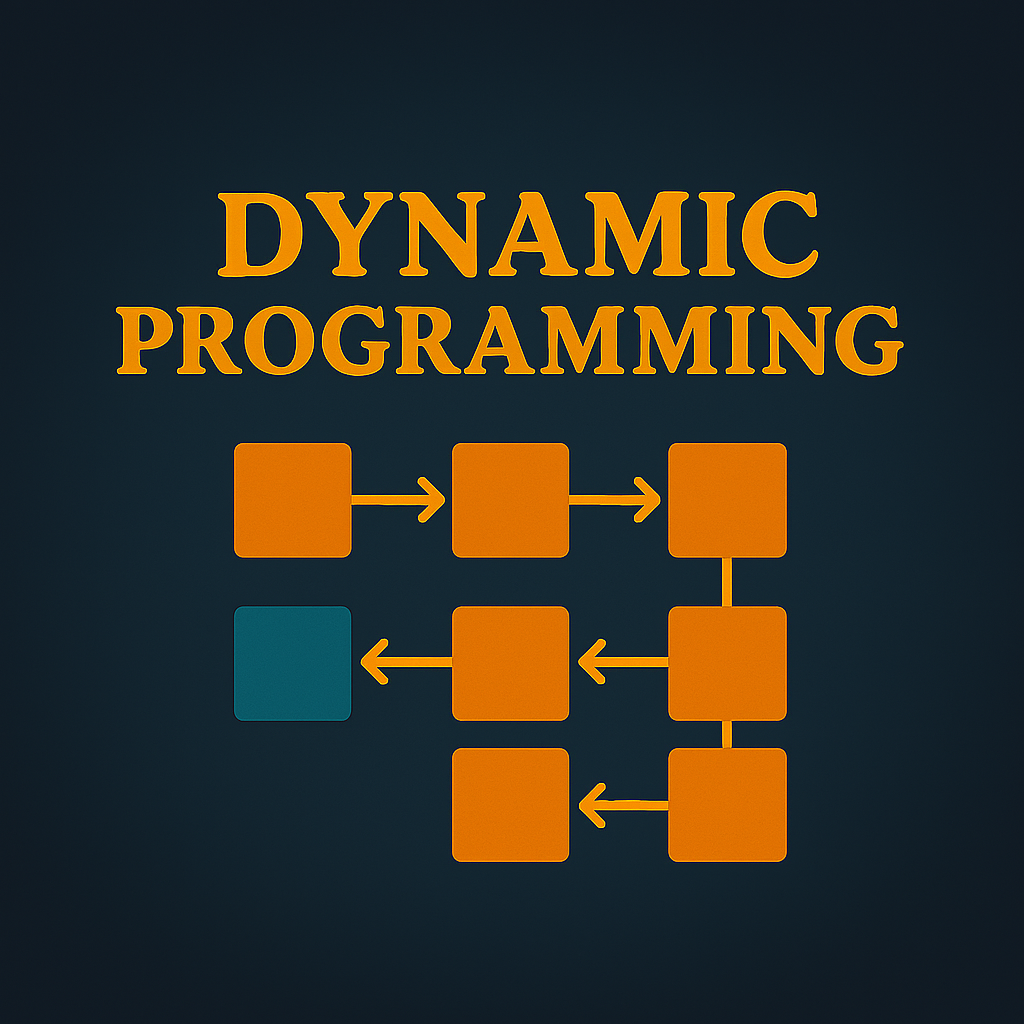
\includegraphics[height=13.88cm, width=17cm, keepaspectratio]{Pics/dp.png}
\end{center}

\chapter{Essential Dynamic Programming Techniques}
\phantomsection                      % <-- creates a hyperlink anchor
\label{sec:dp}
\begin{itemize}[leftmargin=*]
    \item \textbf{Core Principles:}
    \begin{itemize}
        \item Optimal Substructure: Solution to problem contains optimal solutions to subproblems
        \item Overlapping Subproblems: Same subproblems are solved multiple times in naive recursion
        \item Memoization vs Tabulation: Top-down (recursive + cache) vs Bottom-up (iterative)
        \item State Definition: Clearly define what each DP state represents
        \item Base Cases: Identify the simplest cases that don't require further recursion
    \end{itemize}

    \item \textbf{DP Design Process:}
    \begin{itemize}
        \item Step 1: Identify if problem has optimal substructure
        \item Step 2: Define state variables and their meaning
        \item Step 3: Write recurrence relation
        \item Step 4: Identify base cases
        \item Step 5: Determine order of computation (for tabulation)
        \item Step 6: Optimize space if possible
    \end{itemize}
\end{itemize}

\begin{itemize}[leftmargin=*]
    \item \textbf{Linear DP:}
    \begin{itemize}
        \item Fibonacci Pattern: $dp[i] = dp[i-1] + dp[i-2]$
        \item House Robber Pattern: $dp[i] = \max(dp[i-1], dp[i-2] + arr[i])$
        \item Climbing Stairs: Ways to reach position $i$ from previous positions
        \item Maximum Subarray: Kadane's algorithm as DP problem
        \item Coin Change: Minimum coins needed for amount $i$
    \end{itemize}

    \item \textbf{Grid DP:}
    \begin{itemize}
        \item Path Counting: $dp[i][j] = dp[i-1][j] + dp[i][j-1]$
        \item Minimum Path Sum: $dp[i][j] = \min(dp[i-1][j], dp[i][j-1]) + grid[i][j]$
        \item Unique Paths with Obstacles: Handle blocked cells in path counting
        \item Dungeon Game: Work backwards from bottom-right to top-left
        \item Cherry Pickup: Two paths simultaneously through grid
    \end{itemize}

    \item \textbf{String DP:}
    \begin{itemize}
        \item Longest Common Subsequence: $dp[i][j]$ for strings up to position $i,j$
        \item Edit Distance: Minimum operations to transform one string to another
        \item Palindrome Problems: Check/count palindromic subsequences
        \item String Matching: Pattern matching with wildcards
        \item Word Break: Check if string can be segmented using dictionary
    \end{itemize}
\end{itemize}

\begin{itemize}[leftmargin=*]
    \item \textbf{Knapsack Variations:}
    \begin{itemize}
        \item 0/1 Knapsack: Each item can be taken at most once
        \item Unbounded Knapsack: Unlimited quantity of each item
        \item Bounded Knapsack: Limited quantity of each item
        \item Multiple Knapsack: Multiple knapsacks with different capacities
        \item Subset Sum: Special case where values equal weights
    \end{itemize}

    \item \textbf{Interval DP:}
    \begin{itemize}
        \item Matrix Chain Multiplication: Optimal parenthesization
        \item Palindrome Partitioning: Minimum cuts to make all palindromes
        \item Burst Balloons: Optimal order to burst balloons
        \item Optimal BST: Minimize search cost in binary search tree
        \item State: $dp[i][j]$ represents optimal solution for interval $[i,j]$
    \end{itemize}

    \item \textbf{Tree DP:}
    \begin{itemize}
        \item Subtree Problems: Each node's answer depends on its children
        \item Binary Tree Maximum Path Sum: Path can start/end at any node
        \item House Robber III: Rob houses arranged in binary tree
        \item Tree Diameter: Longest path between any two nodes
        \item Rerooting Technique: Compute answer for each node as root
    \end{itemize}

    \item \textbf{Digit DP:}
    \begin{itemize}
        \item Count Numbers with Property: Count numbers in range with specific digits
        \item State Parameters: Position, tight constraint, started flag
        \item Tight Constraint: Whether current prefix forces us to stay within bounds
        \item Leading Zeros: Handle numbers with different digit counts
        \item Sum of Digits: Problems involving digit sum constraints
    \end{itemize}

    \item \textbf{Bitmask DP:}
    \begin{itemize}
        \item Traveling Salesman: Visit all cities with minimum cost
        \item Assignment Problems: Assign tasks to workers optimally
        \item State Representation: Use bitmask to represent subset of items
        \item SOS DP: Sum over subsets dynamic programming
        \item Hamiltonian Path: Find path visiting all vertices exactly once
    \end{itemize}
\end{itemize}

\begin{itemize}[leftmargin=*]
    \item \textbf{Space Optimization:}
    \begin{itemize}
        \item Rolling Array: When current state depends only on previous row/column
        \item 1D to 2D Reduction: Reduce 2D DP to 1D when possible
        \item Coordinate Compression: When state space is sparse but large
        \item Memory Efficient: Process states in specific order to reuse memory
        \item Backwards Iteration: Sometimes needed to avoid overwriting needed values
    \end{itemize}

    \item \textbf{Time Optimization:}
    \begin{itemize}
        \item Matrix Exponentiation: For linear recurrences with large $n$
        \item Convex Hull Trick: Optimize DP with linear functions
        \item Divide and Conquer DP: When recurrence has specific monotonicity
        \item Knuth-Yao Optimization: For quadrilateral inequality problems
        \item Slope Trick: Represent DP function as piecewise linear
    \end{itemize}
\end{itemize}

\begin{itemize}[leftmargin=*]
    \item \textbf{DP Indicators:}
    \begin{itemize}
        \item Optimization Problems: Find minimum/maximum value
        \item Counting Problems: Count number of ways to do something
        \item Decision Problems: Yes/No questions with subproblem structure
        \item Recursive Structure: Problem can be broken into similar subproblems
        \item Choices at Each Step: At each step, you make a choice affecting future
    \end{itemize}

    \item \textbf{When NOT to Use DP:}
    \begin{itemize}
        \item Greedy Suffices: When greedy choice leads to optimal solution
        \item No Overlapping Subproblems: If subproblems don't repeat
        \item Exponential State Space: When memoization table becomes too large
        \item Simple Math Formula: When closed-form solution exists
        \item Graph Problems: When BFS/DFS is more appropriate
    \end{itemize}
\end{itemize}

\begin{itemize}[leftmargin=*]
    \item \textbf{State Variable Selection:}
    \begin{itemize}
        \item Position-based: Current position in array/string/grid
        \item Value-based: Current sum, product, or accumulated value
        \item Choice-based: What was the last choice made
        \item Constraint-based: Remaining capacity, budget, or limit
        \item Flag-based: Boolean flags for special conditions
    \end{itemize}

    \item \textbf{Multi-dimensional States:}
    \begin{itemize}
        \item 2D DP: Two changing parameters (position, remaining capacity)
        \item 3D DP: Three parameters (two strings + operation count)
        \item Bitmask States: When subset of items needs to be tracked
        \item State Compression: Combine multiple variables into single state
    \end{itemize}
\end{itemize}

\begin{itemize}[leftmargin=*]
    \item \textbf{Common Recurrence Types:}
    \begin{itemize}
        \item Addition: $dp[i] = dp[i-1] + dp[i-2]$ (Fibonacci-like)
        \item Minimum/Maximum: $dp[i] = \min/\max(dp[i-1] + cost, dp[i-2] + cost)$
        \item Multiplication: $dp[i] = dp[i-1] \times dp[i-2]$ (rare but exists)
        \item Conditional: Different recurrence based on current element
        \item Range-based: $dp[i] = \min_{j < i}(dp[j] + cost(j,i))$
    \end{itemize}

    \item \textbf{Boundary Conditions:}
    \begin{itemize}
        \item Base Cases: Define values for smallest valid inputs
        \item Invalid States: Handle states that shouldn't be reached
        \item Edge Cases: First/last elements often need special handling
        \item Initialization: Some states need non-zero initial values
        \item Sentinels: Use dummy values to simplify boundary checking
    \end{itemize}
\end{itemize}

\begin{itemize}[leftmargin=*]
    \item \textbf{Implementation Strategie Top-Down (Memoization):}
    \begin{itemize}
        \item Recursive Function: Write natural recursive solution first
        \item Memoization Table: Cache results to avoid recomputation
        \item Parameter Mapping: Map function parameters to array indices
        \item Return vs Reference: Decide whether to return value or modify reference
        \item Stack Overflow: Watch out for deep recursion limits
    \end{itemize}

    \item \textbf{Bottom-Up (Tabulation):}
    \begin{itemize}
        \item Iteration Order: Ensure dependencies are computed before use
        \item Array Initialization: Initialize DP table with appropriate values (Generally reverse of recursive calls)
        \item Loop Structure: Nested loops for multi-dimensional DP (bottom-up)
        \item State Transitions: Implement recurrence relation in loops(usually same as recursive version)
        \item Final Answer: Extract answer from appropriate DP state(by which recursion was called)
    \end{itemize}
\end{itemize}
\begin{itemize}[leftmargin=*]
    \item \textbf{DP-Specific Debugging:}
    \begin{itemize}
        \item Small Test Cases: Start with minimal input size
        \item Base Case Verification: Ensure base cases are correct
        \item State Printing: Print DP table to visualize computation
        \item Recurrence Checking: Manually verify few state transitions
        \item Boundary Testing: Test edge cases thoroughly
    \end{itemize}

    \item \textbf{Common DP Mistakes:}
    \begin{itemize}
        \item Wrong State Definition: State doesn't capture all necessary information
        \item Incorrect Base Cases: Base cases don't match problem requirements
        \item Order Dependency: Computing states before their dependencies
        \item Index Errors: Off-by-one errors in array indexing
        \item Overflow Issues: Integer overflow in intermediate calculations
    \end{itemize}
\end{itemize}
\begin{itemize}[leftmargin=*]
    \item \textbf{Problem Analysis:}
    \begin{itemize}
        \item Constraint Analysis: Use constraints to estimate DP table size
        \item Pattern Recognition: Quickly identify known DP patterns
        \item Brute Force First: Start with recursive solution, then optimize
        \item State Space Estimation: Calculate memory requirements early
        \item Time Complexity: Estimate time complexity from state count
    \end{itemize}

    \item \textbf{Implementation Speed:}
    \begin{itemize}
        \item Template Preparation: Have templates for common DP patterns
        \item Macro Usage: Define macros for loop structures and common operations
        \item Fast I/O: Use fast input/output for large datasets
        \item Memory Declaration: Declare DP arrays globally to avoid stack overflow
        \item Code Reuse: Adapt similar problem solutions when possible
    \end{itemize}

    \item \textbf{Problem Variants:}
    \begin{itemize}
        \item Path Reconstruction: Sometimes you need to find actual solution, not just value
        \item Multiple Queries: Precompute DP table for answering multiple queries
        \item Online DP: Handle dynamic updates to input
        \item Probability DP: Expected value calculations using DP
        \item Game Theory DP: Minimax problems with optimal play
    \end{itemize}
\end{itemize}

\begin{itemize}[leftmargin=*]
    \item \textbf{Mathematical Optimization:}
    \begin{itemize}
        \item Lagrange Multipliers: For constrained optimization problems
        \item Generating Functions: Convert DP recurrence to algebraic form
        \item Linear Programming: When DP can be formulated as LP
        \item Probability Theory: For expected value DP problems
        \item Combinatorics: For counting problems with DP
    \end{itemize}

    \item \textbf{Data Structure Integration:}
    \begin{itemize}
        \item Segment Trees: For range query DP optimizations
        \item Binary Indexed Trees: For efficient range sum updates
        \item Priority Queues: For maintaining optimal choices
        \item Deque Optimization: For sliding window DP problems
        \item Hash Tables: For state compression and memoization
    \end{itemize}
\end{itemize}


\section{Dynamic Programming-Based DSA Problems Summary Table}
\begin{longtable}{|>{\raggedright\arraybackslash}p{3.2cm}|>{\columncolor{c2}\centering\arraybackslash}p{2.5cm}|>{\columncolor{c3}\raggedright\arraybackslash}p{4.3cm}|>{\columncolor{c4}\raggedright\arraybackslash}p{3.5cm}|>{\columncolor{c5}\color{white}\raggedright\arraybackslash}p{3.5cm}|}
\hline
\rowcolor{rclr}
\textbf{Problem Name} & \textbf{Time Complexity} & \textbf{Idea to Solve} & \textbf{Optimization Tip} & \textbf{Edge Cases} \\
\hline
\endfirsthead
\hline
\rowcolor{rclr}
\textbf{Problem Name} & \textbf{Time Complexity} & \textbf{Idea to Solve} & \textbf{Optimization Tip} & \textbf{Edge Cases} \\
\hline
\endhead
Binomial Coefficient & $O(nk)$ & $C(n, k) = C(n-1, k-1) + C(n-1, k)$ & Use 1D array for space optimization. & k = 0 or k = n \\
\hline
Minimum Jumps to Reach End & $O(n^2)$ & $dp[i] = \min(dp[j] + 1)$ for all $j$ where $j + arr[j] \geq i$ & Greedy + DP for faster solution. & 0 at start, unreachable end \\
\hline
Longest Increasing Subsequence & $O(n^2)$ or $O(n \log n)$ & $dp[i] = \max(dp[j] + 1)$ for all $j < i$ and $arr[j] < arr[i]$ & Use Binary Search for $O(n \log n)$ & Strict vs non-strict LIS \\
\hline
Longest Increasing Subsequence (LIS) in $O(n \log n)$ & $O(n \log n)$ & Maintain tail array, use binary search to find correct position of current element & Patience sorting idea; track indices for printing LIS & All decreasing or equal elements \\
\hline
Number of Longest Increasing Subseq. & $O(n^2)$ & Track length and count arrays; update both while scanning & Count ways for each LIS length & All elements same \\
\hline
Print All LIS & $O(n^2)$ & DP for LIS + backtrack all paths matching LIS length & Use memoized backtracking tree & Multiple LIS of same length \\
\hline
Longest Divisible Subset & $O(n^2)$ & Sort + apply DP if $a \% b == 0$ or $b \% a == 0$ & Maintain prev index for reconstruction & All primes or no pair \\
\hline
Minimum Deletions to Make Array Sorted & $O(n^2)$ & $n - \text{LIS}(arr)$ is answer & Use LIS DP for longest sorted subarray & Already sorted or all same \\
\hline
Maximum Sum Increasing Subsequence & $O(n^2)$ & Replace LIS length DP with sum DP & Track current sum, not length & All elements negative \\
\hline
Maximum Length Bitonic Subsequence & $O(n^2)$ & Compute LIS from left, LDS from right; combine & $bitonic[i] = LIS[i] + LDS[i] - 1$ & All increasing or decreasing \\
\hline
Building Bridges (Max Bridges without Crossing) & $O(n \log n)$ & Sort by one coordinate, apply LIS on other & Classic LIS in disguise & Same x or y coordinate \\
\hline
Stack of Boxes (W, H, D) & $O(n^2)$ & Sort boxes by dimension; LIS on valid stackable boxes & Memoize max height for each box as base & Boxes with same dimensions \\
\hline
0-1 Knapsack & $O(nW)$ & $dp[i][w] = \max(dp[i-1][w], val[i] + dp[i-1][w-wt[i]])$ & Use 1D DP with reverse loop. & Zero capacity or no items \\
\hline
Subset Sum & $O(n \cdot sum)$ & $dp[i][j] = dp[i-1][j]$ or $dp[i-1][j - arr[i]]$ & Use 1D boolean DP array in reverse loop (s to a[i]) & sum = 0 or negative numbers \\
\hline
Equal Sum Partition & $O(n \cdot sum)$ & Reduce to Subset Sum with $sum/2$ & Return false if total sum is odd & Odd total sum \\
\hline
Count of Subsets with Given Sum & $O(n \cdot sum)$ & $dp[i][j] = dp[i-1][j] + dp[i-1][j - arr[i]]$ & Use 1D array for space, modulo if needed & sum = 0 or duplicates \\
\hline
Minimum Subset Sum Difference & $O(n \cdot sum)$ & Subset Sum variation: find closest sum $\leq \text{total}/2$ & Track all reachable subset sums & All elements equal or one element \\
\hline
Target Sum(Number of subset with given difference) & $O(n \cdot sum)$ & Count subsets with sum = $(S + total)/2$ & Convert to subset sum count problem & S > total sum or not integer \\
\hline

Longest Common Subsequence & $O(nm)$ & $dp[i][j] = dp[i-1][j-1]+1$ if match else $\max(dp[i-1][j], dp[i][j-1])$ & Use only two rows for space. & One string empty \\
\hline
Printing LCS & $O(nm)$ & Backtrack from $dp[n][m]$ while building string from bottom right move diagonally if matches if not max of top or left & Use reverse of backtracking path & Multiple LCS of same length \\
\hline
Difference Utility (Min Insert + Delete) & $O(nm)$ & LCS-based: Insertions = $m - \text{LCS}$, Deletions = $n - \text{LCS}$ & Use 1D DP if only lengths needed. & One string empty \\
\hline
Minimum Insertions and Deletions to Convert & $O(nm)$ & Same as above: Use LCS of $s1$, $s2$ & Optimize insert/delete count together & Identical strings \\
\hline
Shortest Common Supersequence & $O(nm)$ & $len(SCS) = n + m - \text{LCS}$ & Use LCS table to reconstruct SCS. & One string empty \\
\hline
Print SCS & $O(n \cdot m)$ & Use LCS to reconstruct: if same take once, else take from where max(dp) & Backtrack from LCS table & Empty strings \\
\hline
Longest Repeating Subsequence & $O(n^2)$ & LCS of string with itself, but $i \neq j$ & Modify LCS DP to skip same index match & All characters same or none repeated \\
\hline
Longest Repeating Substring (DP) & $O(n^2)$ & LCS with same string, but $i \neq j$: \newline $dp[i][j] = dp[i-1][j-1]+1$ if $s[i]=s[j]$ & Track max length only & All distinct characters \\
\hline
Longest Palindromic Subsequence & $O(n^2)$ & LCS of string with its reverse & Use standard LCS on $s$ and $rev(s)$ & Palindromic or single character string \\
\hline

Length of Largest Subsequence of A which is Substring in B & $O(n \cdot m)$ & DP where $dp[i][j] = dp[i-1][j-1]+1$ if $a[i]=b[j]$ else 0, track max & Reset if mismatch & Subsequence order mismatch \\
\hline
Subsequence Pattern Matching(if a is present in b) & $O(n \cdot m)$ & Count ways $dp[i][j] = dp[i-1][j-1] + dp[i][j-1]$ if match else $dp[i][j-1]$ & 1D array if needed (len(LPS)==len(a) is sufficient)& a empty, multiple matches \\
\hline
Count of Subsequences of a in b & $O(n \cdot m)$ & Same as above; treat a as pattern and b as text & Initialize first row with 1s (can be done using just 1 1D array) & a longer than b \\
\hline
Longest Palindromic Substring & $O(n^2)$ & $dp[i][j] = true$ if $s[i] = s[j]$ and $dp[i+1][j-1]$ is true & Expand from center for $O(n^2)$ & All same char, length = 1 \\
\hline
Count of Palindromic Substrings & $O(n^2)$ & Count all $(i,j)$ where $s[i..j]$ is palindrome via DP or expand method & Expand around center is simpler & Single chars count too \\
\hline
Minimum Insertions to Make Palindrome & $O(n^2)$ & $dp[i][j] = dp[i+1][j-1]$ if match else $1 + \min(dp[i+1][j], dp[i][j-1])$ & Convert to LPS: $n - LPS$ & Already a palindrome \\
\hline
Minimum Deletions to Make Palindrome & $O(n^2)$ & $n - \text{LPS}(s)$ where LPS = LCS(s, rev(s)) & Use LCS with reverse string & All characters distinct \\
\hline
Edit Distance & $O(nm)$ & $dp[i][j] = 1 + \min(\text{insert, remove, replace})$ & 2 rows only needed. & One string empty \\
\hline
Optimal Strategy for Game (Choose boundary) & $O(n^2)$ & $dp[i][j] = \max(\text{val}_i + \min(dp[i+2][j], dp[i+1][j-1]),\; \text{val}_j + \min(dp[i][j-2], dp[i+1][j-1]))$ & Fill diagonally using gap method & One or two elements only \\
\hline
Count BSTs with $n$ Keys (Catalan Number) & $O(n^2)$ & $dp[n] = \sum_{i=0}^{n-1} dp[i] \cdot dp[n-1-i]$ & Use closed-form: $C_n = \frac{1}{n+1} \binom{2n}{n}$ for large $n$ & $n = 0$ or $n = 1$ \\
\hline
Max Sum with No Two Consecutive & $O(n)$ & $dp[i] = \max(dp[i-1], arr[i] + dp[i-2])$ & 2 variables (prev, prev2) instead of array & Negative numbers \\
\hline
Allocate Minimum Pages & $O(n \cdot k \cdot \log(sum(pages[])$ & Binary search on answer + greedy check if allocation is feasible with mid pages & Minimize max load among partitions & Pages $>$ total or students $>$ books \\
\hline
Unbounded Knapsack & $O(n \cdot W)$ & $dp[i][j] = \max(dp[i-1][j], val[i] + dp[i][j - wt[i]])$ & Use 1D array (forward loop on $j$) & All weights $>$ capacity \\
\hline
Rod Cutting Problem & $O(n \cdot n)$ & $dp[i][j] = \max(dp[i-1][j], price[i-1] + dp[i][j-i])$ & Identical to unbounded knapsack & Length not divisible \\
\hline
Coin Change (Total Ways) & $O(n \cdot sum)$ & $dp[i][j] = dp[i-1][j] + dp[i][j - coin]$ & 1D array suffices using forward loop & No solution or coin = 1 only \\
\hline
Maximum Cuts & $O(n)$ & $dp[i] = \max(dp[i-x], dp[i-y], dp[i-z]) + 1$ if valid & Initialize with -1 to track impossible. & No valid cuts \\
\hline
Minimum Coins to Make Value & $O(n \cdot sum)$ & $dp[i] = \min(dp[i], dp[i-coin] + 1)$ & Use INT\_MAX-1 to avoid overflow. & Value can’t be made \\
Matrix Chain Multiplication (MCM) & $O(n^3)$ & $dp[i][j] = \min_{k=i}^{j-1}(dp[i][k] + dp[k+1][j] + cost)$ & Use gap-based diagonal filling & No matrix to multiply or one matrix \\
\hline
Printing MCM & $O(n^3)$ & Same as MCM, maintain a `bracket[][]` matrix to track $k$ & Recursively print brackets from matrix & Optimal split at multiple $k$ \\
\hline
Boolean Parenthesization (Evaluate to True) & $O(n^3)$ & $T[i][j] = \sum_k$ ways with op, combine true/false & Memoize $(i,j,True/False)$ state & All True or all False cases \\
\hline
Min/Max Value of Expression & $O(n^3)$ & $dp[i][j] = \min/\max$ over all $k$: combine left and right based on operator & Maintain min/max matrices separately & Operator only one type \\
\hline
Palindrome Partitioning (Min Cuts) & $O(n^3)$ & $dp[i][j] = 0$ if palindrome, else $\min_{k=i}^{j-1}(dp[i][k] + dp[k+1][j] + 1)$ & Precompute isPalindrome table & Already palindrome string \\
\hline
Palindrome Partitioning (Min Cuts) & $O(n^2)$ & Instead of calculating dp[i] separately we can do it with the $P[j][i]$ itself & Precompute isPalindrome table & Already palindrome string \\
\hline
Egg Dropping Puzzle & $O(n \cdot k^2)$ & $dp[e][f] = \min_{x=1}^{f} (1 + \max(dp[e-1][x-1], dp[e][f-x]))$ & Use binary search on floor for $O(n \cdot k \log k)$ & 1 egg or 1 floor \\
\hline
Buy \& Sell Stock II (Infinite Tx) & $O(n)$ & Greedy: sum of all positive differences & Track only increasing slopes & Always decreasing prices \\
\hline
Buy \& Sell Stock IV (At most K Tx) & $O(k \cdot n)$ & $dp[i][j] = \max(dp[i][j-1], prices[j] - min)$ & Use 1D DP if optimizing space & k > n/2 acts as infinite tx \\
\hline
Buy \& Sell with Cool Down & $O(n)$ & 3 states: hold, sold, cooldown; recurrence from prev day & Use rolling vars instead of arrays & Cooldown on 1st day \\
\hline
Buy \& Sell with Transaction Fee & $O(n)$ & State: hold or cash; use recurrence on transition with fee & Linear scan with 2 variables & Fee > all profit \\
\hline

Min Cost to Cut Stick & $O(n^3)$ & Add 0 and len, sort cuts → DP: \newline $dp[i][j] = \min(dp[i][j], dp[i][k] + dp[k][j] + cost)$ & Memoize overlapping intervals & No cuts or cuts at ends \\
\hline
isPalindrome(i,j) Preprocessing & $O(n^2)$ & $dp[i][j] = s[i] == s[j] \land dp[i+1][j-1]$ & Precompute and use in partitioning & Single character or empty \\
\hline
Palindrome Partitioning II & $O(n^2)$ & DP + isPalindrome table: \newline $dp[i] = \min(dp[j-1]+1)$ if $s[j..i]$ palindrome & Precompute isPalindrome(i,j) & Already a full palindrome \\
\hline
Count Squares in Binary Matrix & $O(nm)$ & $dp[i][j] = 1 + \min(top, left, diag)$ if cell = 1 & Add all dp[i][j] for total count & Isolated 1s \\
\hline
Balloon Burst (Min/Max Coins) & $O(n^3)$ & DP on interval: \newline $dp[i][j] = \max(dp[i][k] + nums[i]*nums[k]*nums[j] + dp[k][j])$ & Add dummy 1s at ends & Only 1 balloon \\
\hline
Book Allocation Problem (DP) & $O(n^2 \cdot k)$ & $dp[i][j] = \min_{p<i}(\max(dp[p][j-1], sum(p+1..i)))$ & Use prefix sums, try binary search on answer for greedy version & Books > students or large books first \\
\hline
\end{longtable}
\clearpage
\newgeometry{margin=1in}
% \documentclass[a4paper,10pt]{article}
% \usepackage[utf8]{inputenc}
% \usepackage{geometry}
% \usepackage{amsmath}
% \usepackage[table]{xcolor}
% \usepackage{colortbl}
% \usepackage{color,soul}
% \geometry{margin=0.8in}
% \usepackage{xcolor}
% \usepackage{tikz}
% \usetikzlibrary{matrix,fit,backgrounds}
% \usepackage{minted}
% \definecolor{bgcolor}{rgb}{0.8, 0.9, 0.5} % 
% \definecolor{bgcolor1}{rgb}{0.95, 0.95, 0.95} % Light Gray
% \definecolor{bgcolor2}{rgb}{0.85, 0.92, 1.0}  % Soft Blue
% \definecolor{bgcolor3}{rgb}{0.9, 0.85, 1.0}   % Light Purple
% \definecolor{bgcolor4}{rgb}{0.95, 0.88, 0.76} % Warm Beige
% \definecolor{bgcolor5}{rgb}{0.8, 0.95, 0.8}   % Gentle Green
% \definecolor{bgcolor6}{rgb}{1.0, 0.87, 0.87}  % Pastel Red
% \definecolor{bgcolor7}{rgb}{0.86, 0.93, 0.83} % Mint Green
% \definecolor{bgcolor8}{rgb}{0.98, 0.85, 0.94} % Soft Pink
% \definecolor{bgcolor9}{rgb}{0.87, 0.94, 0.98} % Sky Blue
% \definecolor{bgcolor10}{rgb}{0.96, 0.96, 0.82} % Pale Yellow
% 
% \begin{document}
\section*{Dynamic Programming Problem Codes}
% 1. Memoization
\subsection*{\textcolor{green}{\textbf{1. Memoization (Top-Down DP)}}}
\rule{\linewidth}{0.5mm}

We start with a recursive solution and use a 2D array \texttt{dp[i][j]} to store intermediate results to avoid recomputation.

\textbf{Recurrence:}
\[
dp[i][j] = \text{some function of }( dp[i-1][j], dp[i-1][j-1], \ldots)
\]
\begin{Verbatim}[fontsize=\small]
int dp[n][m];
int solve(int i, int j)
    if (base case) return value;
    if (dp[i][j] != -1) return dp[i][j];
    return dp[i][j] = f(solve(i-1, j), solve(i-1, j-1), ...);

\end{Verbatim}

% 2. Tabulation
\subsection*{\textcolor{red}{\textbf{2. Tabulation (Bottom-Up 2D DP)}}}
\rule{\linewidth}{0.5mm}

We convert the recursive structure into an iterative one by filling the \texttt{dp} table in a specific order.

\begin{Verbatim}[fontsize=\small]
for (int i = 0; i <= n; ++i) 
    for (int j = 0; j <= m; ++j) 
        if (base case) dp[i][j] = value;
        else dp[i][j] = f(dp[i-1][j], dp[i-1][j-1], ...);
\end{Verbatim}

% 3. 2-Row Optimization
\subsection*{\textcolor{orange}{\textbf{3. Space Optimization to 2 Rows}}}
\rule{\linewidth}{0.5mm}

Since each row only depends on the previous row, we can reduce space from \texttt{O(n*m)} to \texttt{O(2*m)}.

\begin{Verbatim}[fontsize=\small]
int prev[m+1], curr[m+1];
for (int i = 0; i <= n; ++i) 
    for (int j = 0; j <= m; ++j) 
        if (base case) curr[j] = value;
        else curr[j] = f(prev[j], prev[j-1], ...);
    
    swap(prev, curr);
\end{Verbatim}

% 4. 1-Row Optimization
\subsection*{\textcolor{yellow}{\textbf{4. Space Optimization to 1 Row}}}
\rule{\linewidth}{0.5mm}

If updates are done in reverse (right to left), we can reuse a single array.

\begin{Verbatim}[fontsize=\small]
int dp[m+1];
for (int i = 0; i <= n; ++i)
    for (int j = m; j >= 0; --j)
        if (base case) dp[j] = value;
        else dp[j] = f(dp[j], dp[j-1], ...);
    
\end{Verbatim}

% 5. Diagram
\subsection*{\textcolor{blue}{\textbf{5. Transition Diagram}}}
\rule{\linewidth}{0.5mm}

\begin{center}
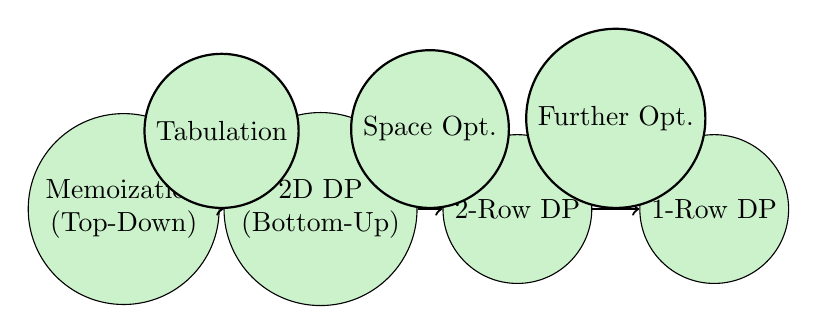
\begin{tikzpicture}[node distance=2.5cm, every node/.style={draw, circle, fill=bgcolor5}, align=center]
\node (A) {Memoization\\(Top-Down)};
\node (B) [right of=A] {2D DP\\(Bottom-Up)};
\node (C) [right of=B] {2-Row DP};
\node (D) [right of=C] {1-Row DP};

\draw[->, thick] (A) -- (B) node[midway, above] {Tabulation};
\draw[->, thick] (B) -- (C) node[midway, above] {Space Opt.};
\draw[->, thick] (C) -- (D) node[midway, above] {Further Opt.};
\end{tikzpicture}
\end{center}

\noindent\textbf{Problem: Binomial Coefficient Pascal's Triangle C(n,k) = C(n−1, k−1) + C(n−1 , k)}
\begin{minted}[
bgcolor=bgcolor2,
frame=lines,
framesep=5mm,
rulecolor=\color{black},
linenos,
numbersep=5pt,
fontsize=\normalsize
]{python}
""" MEMOIZATION : easy to implement using @lru_cache (from functools) or a manual dict"""
from functools import lru_cache

def binomial_coeff(n: int, k: int) -> int:
   
    @lru_cache(maxsize=None)  # Python built-in memoization
    def helper(n, k):
        # Base cases
        if k == 0 or k == n:
            return 1
        if k < 0 or k > n:
            return 0
        # Recursive case
        return helper(n - 1, k - 1) + helper(n - 1, k)
        
    return helper(n, k)
"""" MEMOIZATION : Manual dictionary Space Complexity (Same as above) : O(n * k) """
def binomial_coeff(n: int, k: int) -> int:
    memo = {}

    def helper(n, k):
        if k == 0 or k == n:
            return 1
        if k < 0 or k > n:
            return 0
        if (n, k) in memo:
            return memo[(n, k)]
        memo[(n, k)] = helper(n - 1, k - 1) + helper(n - 1, k)
        return memo[(n, k)]
    
    return helper(n, k)
"""Computes C(n, k) using bottom-up DP(tabulation).Space Complexity: O(n * k)"""
def binomial_coeff(n: int, k: int) -> int:
    # Initialize a (n+1) x (k+1) 2D table with zeros
    dp = [[0] * (k + 1) for _ in range(n + 1)]

    # Fill the table using base cases and recurrence
    for i in range(n + 1):
        for j in range(min(i, k) + 1):  # C(i, j) is 0 when j > i
            if j == 0 or j == i:
                dp[i][j] = 1  # Base cases
            else:
                dp[i][j] = dp[i - 1][j - 1] + dp[i - 1][j]

    return dp[n][k]
""" Computes C(n, k) using bottom-up DP with two rows.Space Complexity: O(2 * k)=O(k)"""
def binomial_coeff(n: int, k: int) -> int:
    prev = [0] * (k + 1)
    curr = [0] * (k + 1)
    
    prev[0] = 1  # Base case: C(0, 0) = 1

    for i in range(1, n + 1):
        curr[0] = 1  # C(i, 0) = 1 for all i
        for j in range(1, min(i, k) + 1):
            curr[j] = prev[j - 1] + prev[j]
        # Swap rows for the next iteration  (no need to copy)
        prev, curr = curr, prev
    
    return prev[k]
""" Computes C(n, k) using most efficient 1 row Tabulation DP Space Complexity: O(k)   """
def binomial_coeff(n: int, k: int) -> int:
    dp = [0] * (k + 1)
    dp[0] = 1  # Base case: C(0,0)=1
    
    # Build the Pascal's Triangle row-by-row
    for i in range(1, n + 1):
        # Update from right to left to avoid overwriting values we still need
        for j in range(min(i, k), 0, -1):
            dp[j] = dp[j] + dp[j - 1]
            # Equivalent to C(i, j) = C(i-1, j) + C(i-1, j-1)
    
    return dp[k]
\end{minted}

\noindent\textbf{Problem: Minimum Jumps to Reach End}
\begin{minted}[
bgcolor=bgcolor5,
frame=lines,
framesep=5mm,
rulecolor=\color{black},
linenos,
numbersep=5pt,
fontsize=\normalsize
]{python}
def min_jumps(arr: List[int]) -> int:
    """
    Finds minimum jumps to reach end of array.
    Time Complexity: O(n^2)       Space Complexity: O(n)
    """
    n = len(arr)
    if n <= 1:
        return 0
    jumps = [float('inf')] * n
    jumps[0] = 0
    
    for i in range(1, n):
        for j in range(i):
            if j + arr[j] >= i and jumps[j] != float('inf'):
                jumps[i] = min(jumps[i], jumps[j] + 1)
    
    return jumps[-1] if jumps[-1] != float('inf') else -1
\end{minted}
\begin{center}
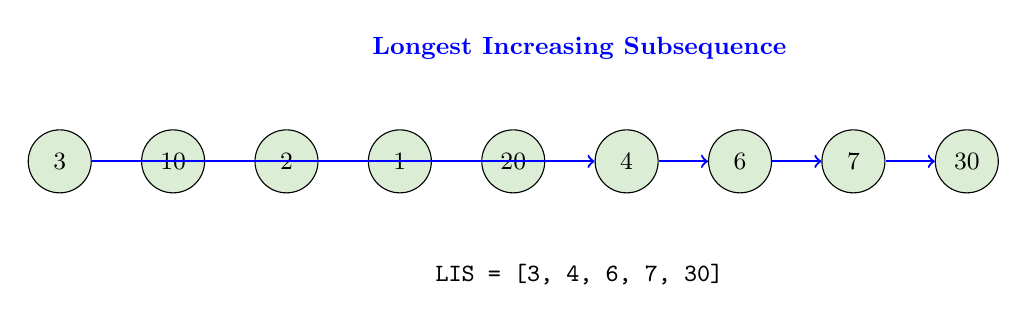
\begin{tikzpicture}[scale=1.2, every node/.style={font=\small}]
    % Sequence of numbers
    \foreach \val/\x in {3/0, 10/1, 2/2, 1/3, 20/4, 4/5, 6/6, 7/7, 30/8} {
        \node[circle, draw=black, fill=bgcolor7, minimum size=8mm] (N\x) at (\x*1.2,0) {\val};
    }

    % Highlighted LIS: 3 → 4 → 6 → 7 → 30
    \foreach \from/\to in {0/5, 5/6, 6/7, 7/8} {
        \draw[->, thick, blue] (N\from) -- (N\to);
    }

    % Labels
    \node at (5.5, 1.2) {\textcolor{blue}{\textbf{Longest Increasing Subsequence}}};
    \node at (5.5, -1.2) {\texttt{LIS = [3, 4, 6, 7, 30]}};

\end{tikzpicture}
\end{center}

\noindent\textbf{Problem: Longest Increasing Subsequence (O(n²))}
\begin{minted}[
bgcolor=bgcolor4,
frame=lines,
framesep=5mm,
rulecolor=\color{black},
linenos,
numbersep=5pt,
fontsize=\normalsize
]{python}
def lis(nums: List[int]) -> int:
    """
    Finds length of longest increasing subsequence (O(n²)).
    Time Complexity: O(n^2)       Space Complexity: O(n)
    """
    n = len(nums)
    dp = [1] * n
    for i in range(1, n):
        for j in range(i):
            if nums[i] > nums[j]:
                dp[i] = max(dp[i], dp[j] + 1)
    return max(dp) if dp else 0
\end{minted}

\noindent\textbf{Problem: Longest Increasing Subsequence (O(n log n))}
\begin{minted}[
bgcolor=bgcolor7,
frame=lines,
framesep=5mm,
rulecolor=\color{black},
linenos,
numbersep=5pt,
fontsize=\normalsize
]{python}
import bisect

def lis_fast(nums: List[int]) -> int:
    """
    Finds length of longest increasing subsequence (O(n log n)).
    Time Complexity: O(n log n)       Space Complexity: O(n)
    """
    tails = []
    for num in nums:
        # Find position to maintain sorted order
        idx = bisect.bisect_left(tails, num)
        if idx == len(tails):
            tails.append(num)
        else:
            tails[idx] = num
    return len(tails)
\end{minted}

\noindent\textbf{Problem: Number of Longest Increasing Subsequences}
\begin{minted}[
bgcolor=bgcolor3,
frame=lines,
framesep=5mm,
rulecolor=\color{black},
linenos,
numbersep=5pt,
fontsize=\normalsize
]{python}
def find_number_of_lis(nums: List[int]) -> int:
    """
    Counts number of longest increasing subsequences.
    Time Complexity: O(n^2)       Space Complexity: O(n)
    """
    n = len(nums)
    if n <= 1: return n
    lengths = [1] * n  # Length of LIS ending at i
    counts = [1] * n   # Count of LIS ending at i
    
    for i in range(n):
        for j in range(i):
            if nums[i] > nums[j]:
                if lengths[j] + 1 > lengths[i]:
                    lengths[i] = lengths[j] + 1
                    counts[i] = counts[j]
                elif lengths[j] + 1 == lengths[i]:
                    counts[i] += counts[j]
    
    max_len = max(lengths)
    return sum(counts[i] for i in range(n) if lengths[i] == max_len)
\end{minted}
\noindent\textbf{Problem: Print All the  Longest Increasing Subsequences}
\begin{minted}[
bgcolor=bgcolor3,
frame=lines,
framesep=5mm,
rulecolor=\color{black},
linenos,
numbersep=5pt,
fontsize=\normalsize
]{python}
def print_all_lis(nums: List[int]) -> List[List[int]]:
"""     Time Complexity: O(n^2 + k*L) k: no of LIS       
        Space Complexity: O(n^2) + recursion stack
"""
    n = len(nums)
    if n == 0:
        return []

    # Phase 1: Compute LIS lengths
    dp = [1] * n
    prev = [[] for _ in range(n)]  # To store predecessors

    for i in range(n):
        for j in range(i):
            if nums[j] < nums[i]:
                if dp[j] + 1 > dp[i]:
                    dp[i] = dp[j] + 1
                    prev[i] = [j]
                elif dp[j] + 1 == dp[i]:
                    prev[i].append(j)

    max_len = max(dp)
    results = []

    # Phase 2: Backtrack to collect all sequences
    def dfs(i, path):
        if not prev[i]:
            if len(path) == max_len - 1:
                results.append([nums[i]] + path)
            return
        for j in prev[i]:
            dfs(j, [nums[i]] + path)

    for i in range(n):
        if dp[i] == max_len:
            dfs(i, [])

    return results
\end{minted}
\noindent\textbf{Problem: Maximum Number of Bridges without crossing}
\\
\begin{figure}[h!]
\centering
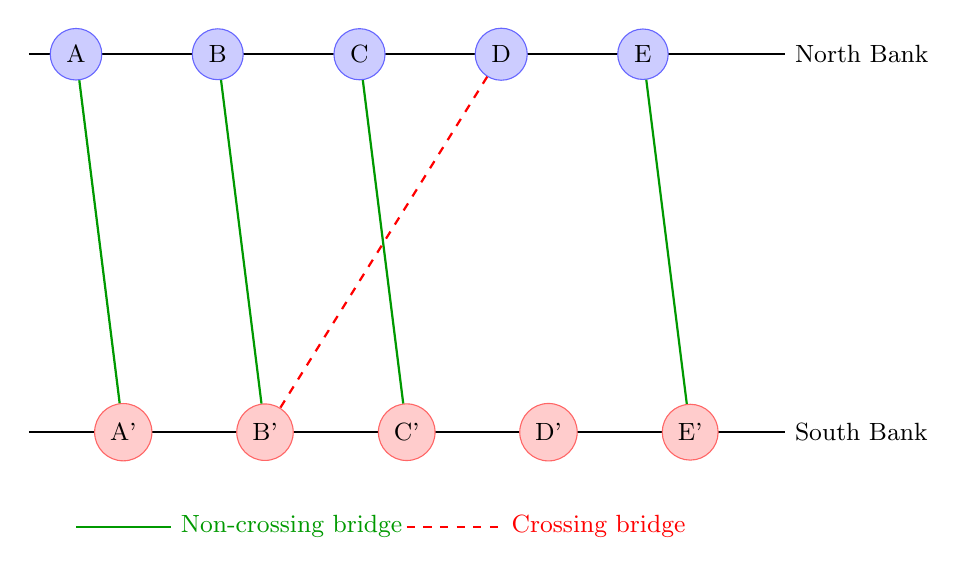
\begin{tikzpicture}[scale=1.2, every node/.style={font=\small}]
    % Draw banks
    \draw[thick] (0,0) -- (8,0) node[right] {South Bank};
    \draw[thick] (0,4) -- (8,4) node[right] {North Bank};

    % North bank cities
    \foreach \x/\name in {0.5/A, 2/B, 3.5/C, 5/D, 6.5/E} {
        \node[circle, draw=blue!60, fill=blue!20, minimum size=6mm] (N\name) at (\x,4) {\name};
    }

    % South bank cities
    \foreach \x/\name in {1/A', 2.5/B', 4/C', 5.5/D', 7/E'} {
        \node[circle, draw=red!60, fill=red!20, minimum size=6mm] (S\name) at (\x,0) {\name};
    }

    % Bridges (some crossing, some non-crossing)
    \draw[thick, green!60!black] (NA) -- (SA');
    \draw[thick, green!60!black] (NB) -- (SB');
    \draw[thick, green!60!black] (NC) -- (SC');
    \draw[thick, red, dashed] (ND) -- (SB'); % crossing
    \draw[thick, green!60!black] (NE) -- (SE');

    % Legend
    \draw[thick, green!60!black] (0.5,-1) -- (1.5,-1) node[right] {Non-crossing bridge};
    \draw[thick, red, dashed] (4,-1) -- (5,-1) node[right] {Crossing bridge};

\end{tikzpicture}
\caption{After sorting by north: [(1,2), (2,4), (3,3), (4,1)] - 
Now find LIS on south: [2, 4, 3, 1] - LIS is [2, 3] - answer is 2}
\end{figure}
\begin{minted}[
bgcolor=bgcolor1,
frame=lines,
framesep=5mm,
rulecolor=\color{black},
linenos,
numbersep=5pt,
fontsize=\normalsize
]{python}
def max_bridges(north: List[int], south: List[int]) -> int:
    """
    Finds the max number of non-crossing bridges.
    Time Complexity: O(n log n)
    """
    pairs = sorted(zip(north, south), key=lambda x: (x[0], x[1]))
    south_sorted = [s for _, s in pairs]

    # Find LIS on south_sorted
    import bisect
    lis = []
    for val in south_sorted:
        idx = bisect.bisect_left(lis, val)
        if idx == len(lis):
            lis.append(val)
        else:
            lis[idx] = val
    return len(lis)
\end{minted}
\noindent\textbf{Problem: 0-1 Knapsack}
\begin{minted}[
bgcolor=bgcolor,
frame=lines,
framesep=5mm,
rulecolor=\color{black},
linenos,
numbersep=5pt,
fontsize=\normalsize
]{python}
def knapSack(W: int, wt: List[int], val: List[int], n: int) -> int:
    """
    Solves 0-1 knapsack problem.
    Time Complexity: O(n*W)       Space Complexity: O(W)
    """
    dp = [0] * (W + 1)
    for i in range(1, n + 1):
        for w in range(W, 0, -1):
            if wt[i - 1] <= w:
                dp[w] = max(dp[w], dp[w - wt[i - 1]] + val[i - 1])
    return dp[W]
\end{minted}

\noindent\textbf{Problem: Subset Sum}
\begin{minted}[
bgcolor=bgcolor7,
frame=lines,
framesep=5mm,
rulecolor=\color{black},
linenos,
numbersep=5pt,
fontsize=\normalsize
]{python}
def subset_sum(nums, target):
    n = len(nums)
    dp = [[False] * (target + 1) for _ in range(n + 1)]
    
    # Base case: zero sum is always possible (empty subset)
    for i in range(n + 1):
        dp[i][0] = True

    for i in range(1, n + 1):
        for j in range(target + 1):
            if j < nums[i - 1]:
                dp[i][j] = dp[i - 1][j]
            else:
                dp[i][j] = dp[i - 1][j] or dp[i - 1][j - nums[i - 1]]

    return dp[n][target]

def subset_sum(nums: List[int], target: int) -> bool:
    """
    Checks if subset exists with given sum.
    Time Complexity: O(n*target)       Space Complexity: O(target)
    """
    dp = [False] * (target + 1)
    dp[0] = True
    for num in nums:
        for j in range(target, num - 1, -1):  # Update backwards
            dp[j] = dp[j] or dp[j - num]
    return dp[target]
\end{minted}

\noindent\textbf{Problem: Count of Subsets with Given Sum}
\begin{minted}[
bgcolor=bgcolor1,
frame=lines,
framesep=5mm,
rulecolor=\color{black},
linenos,
numbersep=5pt,
fontsize=\normalsize
]{python}
def count_subsets(nums: List[int], target: int) -> int:
    """
    Counts subsets with given sum.
    Time Complexity: O(n*target)       Space Complexity: O(target)
    """
    dp = [0] * (target + 1)
    dp[0] = 1
    for num in nums:
        for j in range(target, num - 1, -1):
            dp[j] += dp[j - num]
    return dp[target]
\end{minted}

\noindent\textbf{Problem: Minimum Subset Sum Difference}
\begin{minted}[
bgcolor=bgcolor9,
frame=lines,
framesep=5mm,
rulecolor=\color{black},
linenos,
numbersep=5pt,
fontsize=\normalsize
]{python}
def min_subset_diff(nums: List[int]) -> int:
    """
    Finds minimum difference between two subset sums.
    Time Complexity: O(n*sum)       Space Complexity: O(sum)
    """
    total = sum(nums)
    n = len(nums)
    dp = [False] * (total // 2 + 1)
    dp[0] = True
    
    for num in nums:
        # Update from right to left to avoid reuse of the same number
        for j in range(total // 2, num - 1, -1):
            if dp[j - num]:
                dp[j] = True

    # Find the largest j <= total//2 such that dp[j] is True
    for j in range(total // 2, -1, -1):
        if dp[j]:
            # Total - 2*j gives the minimum difference
            return total - 2 * j
    return float('inf')
\end{minted}

\noindent\textbf{Problem: Longest Common Subsequence}
\begin{center}
\begin{tikzpicture}[every node/.style={anchor=center, minimum size=8mm, font=\bfseries\large}]
    % Define the matrix
    \matrix (m) [matrix of nodes, nodes in empty cells,
        row sep=5mm, column sep=5mm,
        cells={draw, minimum width=6mm, minimum height=6mm}] {
        &   & A & B & C & D & E & F & G \\
        & 0 & 0 & 0 & 0 & 0 & 0 & 0 & 0 \\
      A & 0 & 1 & 1 & 1 & 1 & 1 & 1 & 1 \\
      E & 0 & 1 & 1 & 1 & 1 & 2 & 2 & 2 \\
      C & 0 & 1 & 1 & 2 & 2 & 2 & 2 & 2 \\
      F & 0 & 1 & 1 & 2 & 2 & 2 & 3 & 3 \\
      G & 0 & 1 & 1 & 2 & 2 & 2 & 3 & 4 \\
    };

    % Highlight LCS path: A → C → F → G
    \draw[very thick, green!70!black] (m-2-2.north west) -- (m-3-3.north west) -- (m-4-6.north west)
        -- (m-5-7.north west) -- (m-6-8.north west);

    % Label
    \node[below=1.5cm , text=green!50!black, font=\Huge\bfseries] {LCS = A, C, F, G};

\end{tikzpicture}
\end{center}
\begin{minted}[
bgcolor=bgcolor10,
frame=lines,
framesep=5mm,
rulecolor=\color{black},
linenos,
numbersep=5pt,
fontsize=\normalsize
]{python}
def lcs_length(text1: str, text2: str) -> int:
    m, n = len(text1), len(text2)
    dp = [[0] * (n + 1) for _ in range(m + 1)]

    for i in range(1, m + 1):
        for j in range(1, n + 1):
            if text1[i - 1] == text2[j - 1]:
                dp[i][j] = 1 + dp[i - 1][j - 1]
            else:
                dp[i][j] = max(dp[i - 1][j], dp[i][j - 1])

    return dp[m][n]

def lcs(X: str, Y: str) -> int:
    """
    Finds length of longest common subsequence.
    Time Complexity: O(m*n)       Space Complexity: O(min(m,n))
    """
    m, n = len(X), len(Y)
    if m < n:
        return lcs(Y, X)
    dp = [0] * (n + 1)
    for i in range(1, m + 1):
        prev = 0  # prev keeps track of dp[j-1] from the previous row (dp[i-1][j-1])
        for j in range(1, n + 1):
            temp = dp[j] # temp saves current dp[j] before it gets overwritten.
            if X[i - 1] == Y[j - 1]:
                dp[j] = prev + 1 # LCS between X[0..i-1] and Y[0..j-1]
            else:
                dp[j] = max(dp[j], dp[j - 1]) #dp[j] → value from the previous row (same j) 
                # and dp[j-1] → value to the left in current row
            prev = temp
    return dp[n]
\end{minted}

\noindent\textbf{Problem: Printing LCS}
\begin{minted}[
bgcolor=bgcolor5,
frame=lines,
framesep=5mm,
rulecolor=\color{black},
linenos,
numbersep=5pt,
fontsize=\normalsize
]{python}
def print_lcs(X: str, Y: str) -> str:
    """
    Prints longest common subsequence.
    Time Complexity: O(m*n)       Space Complexity: O(m*n)
    """
    m, n = len(X), len(Y)
    dp = [[0] * (n + 1) for _ in range(m + 1)]
    
    # Build DP table
    for i in range(1, m + 1):
        for j in range(1, n + 1):
            if X[i - 1] == Y[j - 1]:
                dp[i][j] = dp[i - 1][j - 1] + 1
            else:
                dp[i][j] = max(dp[i - 1][j], dp[i][j - 1])
    
    # Backtrack to find LCS
    res = []
    i, j = m, n
    while i > 0 and j > 0:
        if X[i - 1] == Y[j - 1]:
            res.append(X[i - 1])
            i -= 1
            j -= 1
        elif dp[i - 1][j] > dp[i][j - 1]:
            i -= 1
        else:
            j -= 1
    return ''.join(reversed(res))
\end{minted}
\noindent\textbf{Problem: Print SCS (Shortest Common Supersequence)}
\begin{minted}[
bgcolor=bgcolor4,
frame=lines,
framesep=5mm,
rulecolor=\color{black},
linenos,
numbersep=5pt,
fontsize=\normalsize
]{python}
def print_scs(X: str, Y: str) -> str:
    """
    Prints shortest common supersequence of two strings.
    Time Complexity: O(m*n)       Space Complexity: O(m*n)
    """
    m, n = len(X), len(Y)
    dp = [[0]*(n+1) for _ in range(m+1)]
    
    # Build LCS table
    for i in range(1, m+1):
        for j in range(1, n+1):
            if X[i-1] == Y[j-1]:
                dp[i][j] = 1 + dp[i-1][j-1]
            else:
                dp[i][j] = max(dp[i-1][j], dp[i][j-1])
    
    # Backtrack to construct SCS
    res = []
    i, j = m, n
    while i > 0 and j > 0:
        if X[i-1] == Y[j-1]:
            res.append(X[i-1])
            i -= 1
            j -= 1
        elif dp[i-1][j] > dp[i][j-1]:
            res.append(X[i-1])
            i -= 1
        else:
            res.append(Y[j-1])
            j -= 1
    
    # Add remaining characters
    while i > 0:
        res.append(X[i-1])
        i -= 1
    while j > 0:
        res.append(Y[j-1])
        j -= 1
        
    return ''.join(reversed(res))
\end{minted}

\noindent\textbf{Problem: Longest Repeating Subsequence}
\begin{minted}[
bgcolor=bgcolor9,
frame=lines,
framesep=5mm,
rulecolor=\color{black},
linenos,
numbersep=5pt,
fontsize=\normalsize
]{python}
def lrs(s: str) -> int:
    """
    Finds length of longest repeating subsequence.
    Time Complexity: O(n^2)       Space Complexity: O(n^2)
    """
    n = len(s)
    dp = [[0]*(n+1) for _ in range(n+1)]
    
    for i in range(1, n+1):
        for j in range(1, n+1):
            if s[i-1] == s[j-1] and i != j:
                dp[i][j] = 1 + dp[i-1][j-1]
            else:
                dp[i][j] = max(dp[i-1][j], dp[i][j-1])
    return dp[n][n]
\end{minted}

\noindent\textbf{Problem: Longest Repeating Substring (DP) (Also in Binary Search)}
\begin{minted}[
bgcolor=bgcolor8,
frame=lines,
framesep=5mm,
rulecolor=\color{black},
linenos,
numbersep=5pt,
fontsize=\normalsize
]{python}
def lrs_substring(s: str) -> int:
    """
    Finds length of longest repeating substring using DP.
    Time Complexity: O(n^2)       Space Complexity: O(n^2)
    """
    n = len(s)
    dp = [[0]*(n+1) for _ in range(n+1)]
    max_len = 0
    
    for i in range(1, n+1):
        for j in range(1, n+1):
            if s[i-1] == s[j-1] and i != j:
                dp[i][j] = 1 + dp[i-1][j-1]
                max_len = max(max_len, dp[i][j])
            else:
                dp[i][j] = 0
    return max_len
\end{minted}

\noindent\textbf{Problem: Length of Largest Subsequence of A which is Substring in B}
\begin{minted}[
bgcolor=bgcolor3,
frame=lines,
framesep=5mm,
rulecolor=\color{black},
linenos,
numbersep=5pt,
fontsize=\normalsize
]{python}
def max_common_subsequence_substring(A: str, B: str) -> int:
    """
    Finds largest subsequence of A that is substring in B.
    Time Complexity: O(m*n)       Space Complexity: O(n)
    """
    m, n = len(A), len(B)
    max_len = 0
    # dp[j] stores max length ending at j in B
    dp = [0] * (n+1)
    
    for i in range(1, m+1):
        # Traverse backwards to avoid overwriting
        for j in range(n, 0, -1):
            if A[i-1] == B[j-1]:
                dp[j] = 1 + dp[j-1]
                max_len = max(max_len, dp[j])
            else:
                dp[j] = 0  # Reset since it must be substring
    return max_len
\end{minted}

\noindent\textbf{Problem: Subsequence Pattern Matching}
\begin{minted}[
bgcolor=bgcolor,
frame=lines,
framesep=5mm,
rulecolor=\color{black},
linenos,
numbersep=5pt,
fontsize=\normalsize
]{python}
def is_subsequence(a: str, b: str) -> bool:
    """
    Checks if a is subsequence of b.
    Time Complexity: O(n)       Space Complexity: O(1)
    """
    i, j = 0, 0
    while i < len(a) and j < len(b):
        if a[i] == b[j]:
            i += 1
        j += 1
    return i == len(a)
\end{minted}

\noindent\textbf{Problem: Count of Subsequences of a in b}
\begin{minted}[
bgcolor=bgcolor8,
frame=lines,
framesep=5mm,
rulecolor=\color{black},
linenos,
numbersep=5pt,
fontsize=\normalsize
]{python}
def count_subsequences_recursive(a: str, b: str, m: int, n: int) -> int:

    # Base Case: If a is fully traversed, we found a subsequence match
    if m == 0:
        return 1

    # Base Case: If b is fully traversed but a is not, no more matches are possible
    if n == 0:
        return 0

    # If last characters match, we can either include it or skip it
    if a[m - 1] == b[n - 1]:
        # Include the matching character + skip the character
        return (count_subsequences_recursive(a, b, m - 1, n - 1) +
                count_subsequences_recursive(a, b, m, n - 1))
    else:
        # If characters don’t match, skip current character of b
        return count_subsequences_recursive(a, b, m, n - 1)
        
def count_subsequences(a: str, b: str) -> int:
    """
    Counts occurrences of a as subsequence in b.
    Time Complexity: O(m*n)       Space Complexity: O(m)
    """
    m, n = len(a), len(b)
    dp = [0] * (m+1)
    dp[0] = 1  # Empty string has 1 match
    
    for j in range(1, n+1):
        # Traverse backwards to avoid overwriting
        for i in range(m, 0, -1):
            if a[i-1] == b[j-1]:
                dp[i] += dp[i-1]
    return dp[m]
\end{minted}

\noindent\textbf{Problem: Longest Palindromic Substring}
\begin{minted}[
bgcolor=bgcolor7,
frame=lines,
framesep=5mm,
rulecolor=\color{black},
linenos,
numbersep=5pt,
fontsize=\normalsize
]{python}
def longest_palindromic_substring(s: str) -> str:
    """
    Finds longest palindromic substring using DP.
    Time Complexity: O(n^2)       Space Complexity: O(n^2)
    """
    n = len(s)
    dp = [[False]*n for _ in range(n)]
    start, max_len = 0, 1
    
    # All substrings of length 1 are palindromes
    for i in range(n):
        dp[i][i] = True
    
    # Check for length 2
    for i in range(n-1):
        if s[i] == s[i+1]:
            dp[i][i+1] = True
            start = i
            max_len = 2
    
    # Check lengths > 2
    for length in range(3, n+1):
        for i in range(n-length+1):
            j = i+length-1
            if s[i] == s[j] and dp[i+1][j-1]:
                dp[i][j] = True
                if length > max_len:
                    start = i
                    max_len = length
    return s[start:start+max_len]
\end{minted}

\noindent\textbf{Problem: Count of Palindromic Substrings}
\begin{minted}[
bgcolor=bgcolor4,
frame=lines,
framesep=5mm,
rulecolor=\color{black},
linenos,
numbersep=5pt,
fontsize=\normalsize
]{python}
def count_palindromic_substrings(s: str) -> int:
    """
    Counts all palindromic substrings in a string.
    Time Complexity: O(n^2)       Space Complexity: O(n^2)
    """
    n = len(s)
    dp = [[False]*n for _ in range(n)]
    count = 0
    
    for i in range(n):
        dp[i][i] = True
        count += 1
    
    for i in range(n-1):
        if s[i] == s[i+1]:
            dp[i][i+1] = True
            count += 1
    
    for length in range(3, n+1):
        for i in range(n-length+1):
            j = i+length-1
            if s[i] == s[j] and dp[i+1][j-1]:
                dp[i][j] = True
                count += 1
    return count
\end{minted}

\noindent\textbf{Problem: Minimum Insertions to Make Palindrome}
\begin{minted}[
bgcolor=bgcolor3,
frame=lines,
framesep=5mm,
rulecolor=\color{black},
linenos,
numbersep=5pt,
fontsize=\normalsize
]{python}
def min_insertions_recursive(s: str, i: int, j: int) -> int:
    # Base Case: If the substring has 0 or 1 character, it's already a palindrome
    if i >= j:
        return 0

    # If characters match, we can skip both ends
    if s[i] == s[j]:
        return min_insertions_recursive(s, i + 1, j - 1)
    else:
        # If they don't match, insert a character at either end
        # and solve the smaller subproblems, taking the minimal path
        insert_left = min_insertions_recursive(s, i + 1, j)
        insert_right = min_insertions_recursive(s, i, j - 1)
        return 1 + min(insert_left, insert_right)
def min_insertions_palindrome(s: str) -> int:
    """
    Finds minimum insertions to make string palindrome.
    Time Complexity: O(n^2)       Space Complexity: O(n^2)
    """
    n = len(s)
    dp = [[0]*n for _ in range(n)]
    
    for length in range(2, n+1):
        for i in range(n-length+1):
            j = i+length-1
            if s[i] == s[j]:
                dp[i][j] = dp[i+1][j-1]
            else: # characters don't match, insert on either side
                dp[i][j] = 1 + min(dp[i+1][j], dp[i][j-1])
    return dp[0][n-1]
\end{minted}

\noindent\textbf{Problem: Edit Distance}
\begin{minted}[
bgcolor=bgcolor2,
frame=lines,
framesep=5mm,
rulecolor=\color{black},
linenos,
numbersep=5pt,
fontsize=\normalsize
]{python}
def edit_distance(word1: str, word2: str) -> int:
    """
    Computes minimum edit operations (insert, delete, replace) to convert word1 to word2.
    Time Complexity: O(m*n)       Space Complexity: O(min(m,n))
    """
    m, n = len(word1), len(word2)
    if m < n:
        return edit_distance(word2, word1)
    
    dp = [0] * (n+1)
    # Initialize first row
    for j in range(n+1):
        dp[j] = j
    
    for i in range(1, m+1):
        prev = dp[0]
        dp[0] = i
        for j in range(1, n+1):
            temp = dp[j]
            if word1[i-1] == word2[j-1]:
                dp[j] = prev
            else:
                dp[j] = 1 + min(prev, dp[j], dp[j-1])
            prev = temp
    return dp[n]
\end{minted}
\noindent\textbf{Problem: Optimal Strategy for Game}
\begin{minted}[
bgcolor=bgcolor1,
frame=lines,
framesep=5mm,
rulecolor=\color{black},
linenos,
numbersep=5pt,
fontsize=\normalsize
]{python}
def optimal_strategy(arr: List[int]) -> int:
    """
    Maximizes value by choosing ends optimally (picking game).
    Time Complexity: O(n^2)       Space Complexity: O(n^2)
    """
    n = len(arr)
    dp = [[0]*n for _ in range(n)]
    
    for gap in range(n):
        for i in range(n - gap):
            j = i + gap
            x = dp[i+2][j] if i+2 <= j else 0
            y = dp[i+1][j-1] if i+1 <= j-1 else 0
            z = dp[i][j-2] if i <= j-2 else 0
            dp[i][j] = max(arr[i] + min(x, y), arr[j] + min(y, z))
    
    return dp[0][n-1]
\end{minted}

\noindent\textbf{Problem: Count BSTs with n Keys (Catalan Number)}
\begin{minted}[
bgcolor=bgcolor8,
frame=lines,
framesep=5mm,
rulecolor=\color{black},
linenos,
numbersep=5pt,
fontsize=\normalsize
]{python}
def count_bsts(n: int) -> int:
    """
    Counts structurally unique BSTs with n keys (Catalan number).
    Time Complexity: O(n^2)       Space Complexity: O(n)
    """
    dp = [0]*(n+1)
    dp[0] = 1
    for i in range(1, n+1):
        for j in range(i):
            dp[i] += dp[j] * dp[i-j-1]
    return dp[n]
\end{minted}

\noindent\textbf{Problem: Max Sum with No Adjacent Elements}
\begin{minted}[
bgcolor=bgcolor5,
frame=lines,
framesep=5mm,
rulecolor=\color{black},
linenos,
numbersep=5pt,
fontsize=\normalsize
]{python}
def max_sum_non_adjacent(arr: List[int]) -> int:
    """
    Finds maximum sum of non-adjacent elements.
    Time Complexity: O(n)       Space Complexity: O(1)
    """
    incl = 0
    excl = 0
    for num in arr:
        new_incl = excl + num
        excl = max(incl, excl)
        incl = new_incl
    return max(incl, excl)
\end{minted}
\noindent\textbf{Problem: Unbounded Knapsack}
\begin{minted}[
bgcolor=bgcolor10,
frame=lines,
framesep=5mm,
rulecolor=\color{black},
linenos,
numbersep=5pt,
fontsize=\normalsize
]{python}
def unbounded_knapsack_recursive(wt: list, val: list, W: int, n: int) -> int:
    # Base Case: No capacity or no items left
    if W == 0 or n == 0:
        return 0

    # If item can be included
    if wt[n - 1] <= W:
        # Include item (stay at same index to allow repetition)
        include = val[n - 1] + unbounded_knapsack_recursive(wt, val, W - wt[n - 1], n)
        # Exclude item (move to next index)
        exclude = unbounded_knapsack_recursive(wt, val, W, n - 1)
        return max(include, exclude)
    else:
        # Skip item if it can't fit
        return unbounded_knapsack_recursive(wt, val, W, n - 1)
def unbounded_knapsack_by_loop(wt: list, val: list, W: int) -> int:
    # Base case: no capacity left
    if W == 0:
        return 0

    max_val = 0
    # Try every item that fits in the current capacity
    for i in range(len(wt)):
        if wt[i] <= W:
            # Include item i and recur for reduced capacity W - wt[i]
            current = val[i] + unbounded_knapsack_by_loop(wt, val, W - wt[i])
            max_val = max(max_val, current)

    return max_val
def unbounded_knapsack(wt: list, val: list, W: int) -> int:
    n = len(wt)
    # Initialize DP table: dp[i][j] = max value using first i items for capacity j
    dp = [[0] * (W + 1) for _ in range(n + 1)]

    for i in range(1, n + 1):
        for j in range(W + 1):
            if wt[i - 1] <= j:
                # Include or exclude current item (can reuse)
                dp[i][j] = max(dp[i - 1][j], val[i - 1] + dp[i][j - wt[i - 1]])
            else:
                dp[i][j] = dp[i - 1][j]

    return dp[n][W]
def unbounded_knapsack(W: int, wt: List[int], val: List[int]) -> int:
    """
    Solves unbounded knapsack (multiple copies allowed).
    Time Complexity: O(n*W)       Space Complexity: O(W)
    """
    dp = [0]*(W+1)
    for w in range(1, W+1):
        for i in range(len(wt)):
            if wt[i] <= w:
                dp[w] = max(dp[w], dp[w - wt[i]] + val[i])
    return dp[W]
\end{minted}

\noindent\textbf{Problem: Rod Cutting Problem}
\begin{minted}[
bgcolor=bgcolor2,
frame=lines,
framesep=5mm,
rulecolor=\color{black},
linenos,
numbersep=5pt,
fontsize=\normalsize
]{python}
def rod_cutting_recursive(prices: list, n: int) -> int:
    # Base case: no length means no profit
    if n == 0:
        return 0

    max_profit = float('-inf')

    # Try every possible first cut from 1 to n
    for i in range(1, n + 1):
        # prices[i-1] is the price for rod length i
        profit = prices[i - 1] + rod_cutting_recursive(prices, n - i)
        max_profit = max(max_profit, profit)

    return max_profit

def rod_cutting(prices: List[int], n: int) -> int:
    """
    Maximizes profit by cutting rod optimally.
    Time Complexity: O(n^2)       Space Complexity: O(n)
    """
    dp = [0]*(n+1)
    for i in range(1, n+1):
        max_val = float('-inf')
        for j in range(i):
            max_val = max(max_val, prices[j] + dp[i-j-1])
        dp[i] = max_val
    return dp[n]
\end{minted}

\noindent\textbf{Problem: Coin Change (Total Ways)}
\begin{minted}[
bgcolor=bgcolor9,
frame=lines,
framesep=5mm,
rulecolor=\color{black},
linenos,
numbersep=5pt,
fontsize=\normalsize
]{python}
def coin_change_ways(coins: list, n: int, amount: int) -> int:
    # Base Case: If amount is 0, there's one valid way (choose nothing)
    if amount == 0:
        return 1

    # Base Case: If no coins left and amount not 0, no valid way
    if n == 0 and amount > 0:
        return 0

    # If current coin can be used
    if coins[n - 1] <= amount:
        # 1. Include coin[n-1] and stay at same index (unbounded)
        # 2. Exclude coin[n-1] and move to next
        return (coin_change_ways(coins, n, amount - coins[n - 1]) +
                coin_change_ways(coins, n - 1, amount))
    else:
        # Only option: exclude coin[n-1]
        return coin_change_ways(coins, n - 1, amount)
def coin_change_ways(coins: List[int],amount: int) ->int:
    n = len(coins)

    # dp[i][j] = ways to make amount j using first i coins
    dp = [[0] * (amount + 1) for _ in range(n + 1)]

    # Base case: 1 way to form amount 0 (choose nothing)
    for i in range(n + 1):
        dp[i][0] = 1

    # Fill the table row by row
    for i in range(1, n + 1):
        for j in range(amount + 1):
            # Exclude coin[i-1]
            dp[i][j] = dp[i - 1][j]
            # Include coin[i-1] if it fits
            if coins[i - 1] <= j:
                dp[i][j] += dp[i][j - coins[i - 1]]

    return dp[n][amount]
def coin_change_ways(coins: List[int], amount: int) -> int:
    """
    Counts ways to make amount using coins (order matters).
    Time Complexity: O(amount*n)       Space Complexity: O(amount)
    """
    dp = [0]*(amount+1)
    dp[0] = 1
    for coin in coins:
        for j in range(coin, amount+1):
            dp[j] += dp[j - coin] # same as above in consize way
    return dp[amount]
\end{minted}

\noindent\textbf{Problem: Maximum Cuts}
\begin{minted}[
bgcolor=bgcolor3,
frame=lines,
framesep=5mm,
rulecolor=\color{black},
linenos,
numbersep=5pt,
fontsize=\normalsize
]{python}
def max_cuts(n: int, a: int, b: int, c: int) -> int:
    """
    Maximizes cuts of length a, b, c in rod of length n.
    Time Complexity: O(n)       Space Complexity: O(n)
    """
    dp = [-10**9]*(n+1)
    dp[0] = 0
    for i in range(1, n+1):
        if i >= a: dp[i] = max(dp[i], dp[i-a] + 1)
        if i >= b: dp[i] = max(dp[i], dp[i-b] + 1)
        if i >= c: dp[i] = max(dp[i], dp[i-c] + 1)
    return dp[n] if dp[n] >= 0 else -1
\end{minted}

\noindent\textbf{Problem: Minimum Coins to Make Value}
\begin{minted}[
bgcolor=bgcolor4,
frame=lines,
framesep=5mm,
rulecolor=\color{black},
linenos,
numbersep=5pt,
fontsize=\normalsize
]{python}
def min_coins(coins: List[int], amount: int) -> int:
    """
    Finds minimum coins to make amount (inf supply).
    Time Complexity: O(amount*n)       Space Complexity: O(amount)
    """
    dp = [10**9]*(amount+1)
    dp[0] = 0
    for coin in coins:
        for j in range(coin, amount+1):
            dp[j] = min(dp[j], dp[j-coin] + 1)
    return dp[amount] if dp[amount] != 10**9 else -1
\end{minted}

\noindent\textbf{Problem: Buy \& Sell Stock II (Infinite Tx)}
\begin{minted}[
bgcolor=bgcolor7,
frame=lines,
framesep=5mm,
rulecolor=\color{black},
linenos,
numbersep=5pt,
fontsize=\normalsize
]{python}
def get_maximum_profit(prices: List[int]) -> int:
    n = len(prices)
    # dp[ind][buy] = max profit starting at day ind with buy-flag buy
    dp: List[List[int]] = [[-1, -1] for _ in range(n)]
    
    def get_ans(ind: int, buy: int) -> int:
        # Base case: no more days left
        if ind == n:
            return 0
        
        # Return cached result if available
        if dp[ind][buy] != -1:
            return dp[ind][buy]
        
        if buy == 0:
            # Option 1: skip buying today
            skip = get_ans(ind + 1, 0)
            # Option 2: buy today (subtract price), switch to sell-mode
            buy_stock = -prices[ind] + get_ans(ind + 1, 1)
            profit = max(skip, buy_stock)
        else:
            # Option 1: skip selling today
            skip = get_ans(ind + 1, 1)
            # Option 2: sell today (add price), switch to buy-mode
            sell_stock = prices[ind] + get_ans(ind + 1, 0)
            profit = max(skip, sell_stock)
        
        dp[ind][buy] = profit
        return profit
    
    # Start at day 0 with ability to buy
    return get_ans(0, 0)
from typing import List

def max_profit_tabulation(prices: List[int]) -> int:
    """
    Bottom-up 2D DP for unlimited transactions.
    
    dp[ind][0] = max profit from day ind if we can BUY
    dp[ind][1] = max profit from day ind if we can SELL
    """
    n = len(prices)
    # Create dp table with one extra row for the base case (ind == n)
    dp = [[0, 0] for _ in range(n + 1)]

    # Base case: at ind == n (no days left), profit = 0 for both states
    dp[n][0] = dp[n][1] = 0

    # Fill the table backwards from day n-1 down to 0
    for ind in range(n - 1, -1, -1):
        # When we can buy, choose to skip or buy today
        dp[ind][0] = max(
            dp[ind + 1][0],                    # skip buying today
            -prices[ind] + dp[ind + 1][1]      # buy today, then sell-mode
        )
        # When we can sell, choose to skip or sell today
        dp[ind][1] = max(
            dp[ind + 1][1],                    # skip selling today
            prices[ind] + dp[ind + 1][0]       # sell today, then buy-mode
        )

    # Answer: at day 0 with the ability to buy
    return dp[0][0]

def max_profit_infinite(prices: List[int]) -> int:
    """
    Maximizes profit with infinite transactions.
    Time Complexity: O(n)       Space Complexity: O(1)
    """
    profit = 0
    for i in range(1, len(prices)):
        if prices[i] > prices[i-1]:
            profit += prices[i] - prices[i-1]
    return profit
\end{minted}

\noindent\textbf{Problem: Buy \& Sell Stock IV (At most K Tx)}
\begin{minted}[
bgcolor=bgcolor1,
frame=lines,
framesep=5mm,
rulecolor=\color{black},
linenos,
numbersep=5pt,
fontsize=\normalsize
]{python}
def max_profit_recursive(prices: List[int], K: int) -> int:
    n = len(prices)

    @lru_cache(None)
    def dfs(ind: int, buy: int, cap: int) -> int:
        # Base case: no days left or no transactions left
        if ind == n or cap == 0:
            return 0

        # Option 1: skip today
        profit = dfs(ind + 1, buy, cap)

        if buy == 0:
            # Option 2: buy today, switch to sell-state
            profit = max(profit,
                         -prices[ind] + dfs(ind + 1, 1, cap))
        else:
            # Option 2: sell today, consume one transaction
            profit = max(profit,
                         prices[ind] + dfs(ind + 1, 0, cap - 1))

        return profit

    return dfs(0, 0, K) 

def max_profit_dp(prices: List[int], K: int) -> int:
    n = len(prices)
    # dp table: days 0..n, buy=0/1, cap=0..K
    dp = [[[0] * (K + 1) for _ in range(2)] for _ in range(n + 1)]

    # Build backwards from day n-1 to 0
    for ind in range(n - 1, -1, -1):
        for buy in (0, 1):
            for cap in range(1, K + 1):
                # Skip today
                skip = dp[ind + 1][buy][cap]

                if buy == 0:
                    # Buy today
                    take = -prices[ind] + dp[ind + 1][1][cap]
                else:
                    # Sell today
                    take = prices[ind] + dp[ind + 1][0][cap - 1]

                dp[ind][buy][cap] = max(skip, take)

    return dp[0][0][K]

def max_profit_k(k: int, prices: List[int]) -> int:
    """
    Maximizes profit with at most k transactions.
    Time Complexity: O(n*k)       Space Complexity: O(k)
    """
    if not prices or k == 0:
        return 0
    n = len(prices)
    if k >= n//2:
        # Unlimited transactions
        return sum(max(0, prices[i]-prices[i-1]) for i in range(1, n))
    
    # buy[j]: Minimum “net cost” to have executed up to j buys so far
    # profit[j]: Maximum profit after up to j transactions (buy+sell pairs)
    buy = [float('inf')] * (k + 1)
    profit = [0] * (k + 1)

    for price in prices:
        # j = 1..k: progress through transaction counts
        for j in range(1, k + 1):
            # 1) Minimize the effective cost of buying the j-th share
            buy[j] = min(buy[j], price - profit[j - 1])
            # 2) Maximize profit by potentially selling that j-th share today
            profit[j] = max(profit[j], price - buy[j])

    return profit[k]
\end{minted}

\noindent\textbf{Problem: Buy \& Sell with Cool Down}
\begin{minted}[
bgcolor=bgcolor5,
frame=lines,
framesep=5mm,
rulecolor=\color{black},
linenos,
numbersep=5pt,
fontsize=\normalsize
]{python}
def max_profit_cooldown(prices: List[int]) -> int:
    """
    can be simply implemented in dp by changing i+1 to i+2 on selling
    Maximizes profit with 1-day cooldown after sell.
    Time Complexity: O(n)       Space Complexity: O(1)
    """
    n = len(prices)
    if n <= 1:
        return 0
    buy = -prices[0]
    sell = 0
    cooldown = 0
    
    for i in range(1, n):
        prev_buy = buy
        buy = max(buy, cooldown - prices[i])
        cooldown = sell
        sell = max(sell, prev_buy + prices[i])
    return sell
\end{minted}

\noindent\textbf{Problem: Buy \& Sell with Transaction Fee}
\begin{minted}[
bgcolor=bgcolor10,
frame=lines,
framesep=5mm,
rulecolor=\color{black},
linenos,
numbersep=5pt,
fontsize=\normalsize
]{python}
def max_profit_fee(prices: List[int], fee: int) -> int:
    """
    Maximizes profit with transaction fee per trade.
    Can also be simply done using tabulation just -fee on sell.
    Time Complexity: O(n)       Space Complexity: O(1)
    """
    buy = -prices[0]
    sell = 0
    for i in range(1, len(prices)):
        buy = max(buy, sell - prices[i])
        sell = max(sell, buy + prices[i] - fee)
    return sell
\end{minted}
\noindent\textbf{Problem: Matrix Chain Multiplication (MCM)}
\begin{minted}[
bgcolor=bgcolor1,
frame=lines,
framesep=5mm,
rulecolor=\color{black},
linenos,
numbersep=5pt,
fontsize=\normalsize
]{python}
def matrix_chain_mul(dims: List[int]) -> int:
    """
    Calculates minimum scalar multiplications for matrix chain.
    Time Complexity: O(n^3)       Space Complexity: O(n^2)
    """
    n = len(dims) - 1
    dp = [[0]*n for _ in range(n)]
    
    for length in range(2, n+1):
        for i in range(n - length + 1):
            j = i + length - 1
            dp[i][j] = float('inf')
            for k in range(i, j):
                cost = dp[i][k] + dp[k+1][j] + dims[i]*dims[k+1]*dims[j+1]
                if cost < dp[i][j]:
                    dp[i][j] = cost
    return dp[0][n-1]
\end{minted}

\noindent\textbf{Problem: Printing MCM}
\begin{minted}[
bgcolor=bgcolor5,
frame=lines,
framesep=5mm,
rulecolor=\color{black},
linenos,
numbersep=5pt,
fontsize=\normalsize
]{python}
def print_mcm(dims: List[int]) -> str:
    """
    Prints optimal matrix chain multiplication parenthesization.
    Time Complexity: O(n^3)       Space Complexity: O(n^2)
    """
    n = len(dims) - 1
    dp = [[0]*n for _ in range(n)]
    bracket = [[0]*n for _ in range(n)]
    
    for length in range(2, n+1):
        for i in range(n - length + 1):
            j = i + length - 1
            dp[i][j] = float('inf')
            for k in range(i, j):
                cost = dp[i][k] + dp[k+1][j] + dims[i]*dims[k+1]*dims[j+1]
                if cost < dp[i][j]:
                    dp[i][j] = cost
                    bracket[i][j] = k
    
    def build_str(i, j):
        if i == j:
            return f'M{i+1}'
        return f"({build_str(i, bracket[i][j])} × {build_str(bracket[i][j]+1, j)})"
    
    return build_str(0, n-1)
\end{minted}

\noindent\textbf{Problem: Boolean Parenthesization (Evaluate to True)}
\begin{minted}[
bgcolor=bgcolor7,
frame=lines,
framesep=5mm,
rulecolor=\color{black},
linenos,
numbersep=5pt,
fontsize=\normalsize
]{python}
def boolean_parenthesization(symb: List[str], oper: List[str]) -> int:
    """
    Counts ways to parenthesize boolean expression to evaluate True.
    Time Complexity: O(n^3)       Space Complexity: O(n^2)
    """
    n = len(symb)
    T = [[0]*n for _ in range(n)]
    F = [[0]*n for _ in range(n)]
    
    for i in range(n):
        T[i][i] = 1 if symb[i] == 'T' else 0
        F[i][i] = 1 if symb[i] == 'F' else 0
    
    for gap in range(1, n):
        for i in range(n - gap):
            j = i + gap
            T[i][j] = F[i][j] = 0
            for k in range(i, j):
                tik = T[i][k] + F[i][k]      # total ways left subexpr can evaluate
                tkj = T[k+1][j] + F[k+1][j]  # total ways right subexpr can evaluate
                if oper[k] == '&':
                    T[i][j] += T[i][k] * T[k+1][j]   # both sides True
                    F[i][j] += tik * tkj - T[i][k] * T[k+1][j] # all other combinations false
                elif oper[k] == '|':
                    T[i][j] += tik * tkj - F[i][k] * F[k+1][j]
                    F[i][j] += F[i][k] * F[k+1][j]
                elif oper[k] == '^':
                    T[i][j] += T[i][k]*F[k+1][j] + F[i][k]*T[k+1][j]
                    F[i][j] += T[i][k]*T[k+1][j] + F[i][k]*F[k+1][j]
    return T[0][n-1]


def count_ways(i, j, is_true, expr, dp):
    # Base case: invalid range
    if i > j:
        return 0

    # Base case: single character
    if i == j:
        if is_true:
            return 1 if expr[i] == 'T' else 0
        else:
            return 1 if expr[i] == 'F' else 0

    # Memoization check
    if dp[i][j][is_true] != -1:
        return dp[i][j][is_true]

    ways = 0

    # Try all partitions at operator positions (odd indices)
    for ind in range(i + 1, j, 2):
        op = expr[ind]

        # Recursively calculate left and right parts
        lT = count_ways(i, ind - 1, 1, expr, dp)
        lF = count_ways(i, ind - 1, 0, expr, dp)
        rT = count_ways(ind + 1, j, 1, expr, dp)
        rF = count_ways(ind + 1, j, 0, expr, dp)

        if op == '&':
            if is_true:
                ways += (lT * rT) % MOD
            else:
                ways += (lF * rT + lT * rF + lF * rF) % MOD

        elif op == '|':
            if is_true:
                ways += (lT * rT + lT * rF + lF * rT) % MOD
            else:
                ways += (lF * rF) % MOD

        elif op == '^':
            if is_true:
                ways += (lT * rF + lF * rT) % MOD
            else:
                ways += (lT * rT + lF * rF) % MOD

        ways %= MOD  # take modulo at every step

    dp[i][j][is_true] = ways
    return ways

\end{minted}

\noindent\textbf{Problem: Min/Max Value of Expression}
\begin{minted}[
bgcolor=bgcolor4,
frame=lines,
framesep=5mm,
rulecolor=\color{black},
linenos,
numbersep=5pt,
fontsize=\normalsize
]{python}
def min_max_expression(expr: List[str]) -> tuple:
    """
    Finds min and max value of arithmetic expression.
    Time Complexity: O(n^3)       Space Complexity: O(n^2)
    """
    nums = [int(expr[i]) for i in range(0, len(expr), 2)]  # Separate numbers
    ops = [expr[i] for i in range(1, len(expr), 2)]        # Separate operators 
    n = len(nums)
    min_dp = [[float('inf')]*n for _ in range(n)]
    max_dp = [[float('-inf')]*n for _ in range(n)]
    
    for i in range(n):
        min_dp[i][i] = max_dp[i][i] = nums[i]
    
    for gap in range(1, n):
        for i in range(n - gap):
            j = i + gap
            for k in range(i, j):
                a = eval(f"{max_dp[i][k]} {ops[k]} {max_dp[k+1][j]}")
                b = eval(f"{max_dp[i][k]} {ops[k]} {min_dp[k+1][j]}")
                c = eval(f"{min_dp[i][k]} {ops[k]} {max_dp[k+1][j]}")
                d = eval(f"{min_dp[i][k]} {ops[k]} {min_dp[k+1][j]}")
                min_dp[i][j] = min(min_dp[i][j], a, b, c, d)
                max_dp[i][j] = max(max_dp[i][j], a, b, c, d)
    return min_dp[0][n-1], max_dp[0][n-1]
\end{minted}
\noindent\textbf{Problem: isPalindrome(i,j) Preprocessing}
\begin{minted}[
bgcolor=bgcolor2,
frame=lines,
framesep=5mm,
rulecolor=\color{black},
linenos,
numbersep=5pt,
fontsize=\normalsize
]{python}
def preprocess_palindrome(s: str) -> List[List[bool]]:
    """
    Precomputes palindrome substrings for O(1) queries.
    Time Complexity: O(n^2)       Space Complexity: O(n^2)
    """
    n = len(s)
    dp = [[False]*n for _ in range(n)]
    
    for i in range(n):
        dp[i][i] = True
    
    for i in range(n-1):
        dp[i][i+1] = s[i] == s[i+1]
    
    for length in range(3, n+1):
        for i in range(n-length+1):
            j = i+length-1
            dp[i][j] = dp[i+1][j-1] and s[i] == s[j]
    
    return dp
\end{minted}
\noindent\textbf{Problem: Palindrome Partitioning (Min Cuts)}
\begin{minted}[
bgcolor=bgcolor6,
frame=lines,
framesep=5mm,
rulecolor=\color{black},
linenos,
numbersep=5pt,
fontsize=\normalsize
]{python}
def min_cuts_recursive(i, j, s, memo):
    # Base cases
    if i >= j or is_Pal[i][j]:
        return 0

    if memo[i][j] != -1:
        return memo[i][j]

    min_cut = float('inf')

    for k in range(i, j):
        # Only proceed if left part is palindrome (prune unnecessary recursions)
        if is_Pal[i][k]:
            # Recurse for right part s[k+1..j]
            right = min_cuts_recursive(k + 1, j, s, memo)
            min_cut = min(min_cut, 1 + right)

    memo[i][j] = min_cut
    return min_cut
    
def min_cut_palindrome(s: str) -> int:
    """ It is calculating the is_palindrom on the fly very efficient
    Finds minimum cuts for palindrome partitioning.
    Time Complexity: O(n^2)       Space Complexity: O(n^2)
    """
    n = len(s)
    is_pal = [[False] * n for _ in range(n)]
    
    # dp[i] will store the minimum cuts needed for the substring s[0..i]
    dp = [0] * n
    for i in range(n):
        min_cut = i  # maximum cuts needed if no palins found (cut b/w every character)
        # Try all substrings ending at index i and starting at index j (from 0 to i)
        for j in range(i + 1):
            if s[j] == s[i] and (i - j < 2 or is_pal[j + 1][i - 1]):
                is_pal[j][i] = True  # mark substring s[j..i] as palindrome
                if j == 0:   # s[0..i] is palindrome
                    min_cut = 0
                else:
                    # Otherwise, we add 1 cut to the minimum cuts needed for s[0..j-1]
                    min_cut = min(min_cut, dp[j - 1] + 1)
        # Store the minimum cut count for s[0..i]
        dp[i] = min_cut
    return dp[n-1]
    
\end{minted}

\noindent\textbf{Problem: Egg Dropping Puzzle}
\begin{minted}[
bgcolor=bgcolor9,
frame=lines,
framesep=5mm,
rulecolor=\color{black},
linenos,
numbersep=5pt,
fontsize=\normalsize
]{python}
def egg_drop(eggs: int, floors: int) -> int:
    """
    Finds minimum drops to determine critical floor.
    Time Complexity: O(e*f)       Space Complexity: O(e*f)
    """
    dp = [[0]*(floors+1) for _ in range(eggs+1)]
    
    for e in range(1, eggs+1):
        for f in range(1, floors+1):
            if e == 1:
                dp[e][f] = f
            elif f == 1:
                dp[e][f] = 1
            else:
                dp[e][f] = float('inf')
                for k in range(1, f+1):
                    res = 1 + max(dp[e-1][k-1], dp[e][f-k])
                    dp[e][f] = min(dp[e][f], res)
    return dp[eggs][floors]
\end{minted}

\noindent\textbf{Problem: Min Cost to Cut Stick}
\begin{minted}[
bgcolor=bgcolor5,
frame=lines,
framesep=5mm,
rulecolor=\color{black},
linenos,
numbersep=5pt,
fontsize=\normalsize
]{python}
from functools import lru_cache

def minCost(n: int, cuts: list[int]) -> int:
    # Include the endpoints 0 and n in the cuts list
    cuts = [0] + sorted(cuts) + [n]
    m = len(cuts)

    @lru_cache(maxsize=None)
    def dp(i, j):
        # No cuts to be made in this segment
        if i + 1 >= j:
            return 0

        min_cost = float('inf')
        for k in range(i + 1, j):
            cost = cuts[j] - cuts[i]  # Cost of current cut
            left = dp(i, k)           # Cost to cut the left segment
            right = dp(k, j)          # Cost to cut the right segment
            total = cost + left + right
            min_cost = min(min_cost, total)

        return min_cost

    return dp(0, m - 1)

def minCost(n: int, cuts: list[int]) -> int:
""" Tabulated DP Matching Recursive Structure (Reverse i Loop)"""
    # Step 1: Prepare cuts list with endpoints and sort it
    cuts = [0] + sorted(cuts) + [n]
    m = len(cuts)

    # Step 2: Initialize 2D DP table with 0
    dp = [[0] * m for _ in range(m)]

    # Step 3: Fill dp[i][j] where i < j and j - i >= 2
    for i in range(m - 1, -1, -1):         # i goes backwards
        for j in range(i + 2, m):          # j must be at least i + 2
            dp[i][j] = float('inf')
            for k in range(i + 1, j):      # k is the cut position
                cost = cuts[j] - cuts[i]   # current stick length
                dp[i][j] = min(dp[i][j], cost + dp[i][k] + dp[k][j])

    return dp[0][m - 1]

def min_cut_stick(n: int, cuts: List[int]) -> int:
    """
    Calculates minimum cost to cut stick at given positions.
    Time Complexity: O(m^3)       Space Complexity: O(m^2)
    """
    cuts.sort()
    m = len(cuts)
    cuts = [0] + cuts + [n]
    dp = [[0]*(m+2) for _ in range(m+2)]
    
    for length in range(2, m+2):
        for i in range(0, m+2 - length):
            j = i + length
            dp[i][j] = float('inf')
            for k in range(i+1, j):
                cost = (cuts[j] - cuts[i]) + dp[i][k] + dp[k][j]
                dp[i][j] = min(dp[i][j], cost)
    return dp[0][m+1]
\end{minted}

\noindent\textbf{Problem: Count Squares in Binary Matrix}
\begin{minted}[
bgcolor=bgcolor10,
frame=lines,
framesep=5mm,
rulecolor=\color{black},
linenos,
numbersep=5pt,
fontsize=\normalsize
]{python}
def count_squares(matrix: List[List[int]]) -> int:
    """
    Counts all square submatrices with all ones.
    Time Complexity: O(m*n)       Space Complexity: O(1) - in-place modification
    """
    m, n = len(matrix), len(matrix[0])
    count = 0
    
    for i in range(m):
        for j in range(n):
            if matrix[i][j] == 1:
                if i == 0 or j == 0:
                    count += 1
                else:
                    matrix[i][j] = 1 + min(matrix[i-1][j], 
                                          matrix[i][j-1],
                                          matrix[i-1][j-1])
                    count += matrix[i][j]
    return count
\end{minted}

\noindent\textbf{Problem: Balloon Burst (Min/Max Coins)}
\begin{minted}[
bgcolor=bgcolor,
frame=lines,
framesep=5mm,
rulecolor=\color{black},
linenos,
numbersep=5pt,
fontsize=\normalsize
]{python}
def max_coins_balloons(nums: List[int] ) ->int:
"""RECURSIVE """
    nums =[1] + nums + [1]
    n = len(nums)
    @lru_cache(maxsize=None)
    def solve(i,j):
        if i > j : return 0
        ans = 0
        for k in range(i,j+1):
            coins = nums[i-1] * nums[k] * nums[j+1]
            # we have burst all balloons from i to k-1 and from
            # k+1 to j so are left with only these 3 adjacent
            coins += solve(i,k-1)
            coins += solve(k+1,j)
            ans = max(ans,coins)

        return ans


def max_coins_balloons(nums: List[int]) -> int:
    """
    Maximizes coins from bursting balloons.
    Time Complexity: O(n^3)       Space Complexity: O(n^2)
    """
    # Add 1 before and after the original list to simplify edge cases
    # This is because the balloons at the ends are considered as 1 (virtual balloons)
    nums = [1] + nums + [1]
    n = len(nums)
    dp = [[0]*n for _ in range(n)]
    
    # length is the size of the current interval we're solving for
    # start from length 2 because intervals of length 1 can't have any balloons between them
    for length in range(2, n):
        # Move the sliding window of size length across the nums array
        for left in range(0, n - length):
            right = left + length              
            # Try bursting each balloon 'i' between left and right last, and
            # calculate coins gained from this burst plus coins from subproblems
            for i in range(left + 1, right):
                # left and right are the adjacent balloons after bursting all in between
                coins = nums[left] * nums[i] * nums[right]
                # add coins from bursting balloons in the left and right sub-intervals
                coins += dp[left][i] + dp[i][right]
                dp[left][right] = max(dp[left][right], coins)
    
    return dp[0][n - 1]

\end{minted}

\noindent\textbf{Problem: Book Allocation Problem (DP)}
\begin{minted}[
bgcolor=bgcolor5,
frame=lines,
framesep=5mm,
rulecolor=\color{black},
linenos,
numbersep=5pt,
fontsize=\normalsize
]{python}
def book_allocation_dp(books: List[int], m: int) -> int:
    """
    Allocates books using DP (less efficient than binary search).
    Time Complexity: O(m*n^2)       Space Complexity: O(m*n)
    """
    n = len(books)
    if m > n: return -1
    
    dp = [[10**9]*(n+1) for _ in range(m+1)]
    prefix = [0]*(n+1)
    for i in range(1, n+1):
        prefix[i] = prefix[i-1] + books[i-1]
    
    for i in range(1, n+1):
        dp[1][i] = prefix[i]
    
  for k in range(2, m + 1):           # For each number of students from 2 to m
    for i in range(k, n + 1):         # i books(at least k books,each gets atleast one)
        for j in range(k - 1, i):      
# possible partition points, where the previous k-1 students take first j books, j+1 to i to kth student
            dp[k][i] = min(dp[k][i], max(dp[k-1][j], prefix[i] - prefix[j]))
# dp[k-1][j] is minimum possible "maximum pages assigned" when first j books among k-1 students
# prefix[i] - prefix[j] is the total pages in books from j+1 to i, assigned to the kth student
# max(...) represents the worst load (maximum pages) bw previous k-1  and kth student
# We want to minimize this maximum load across all partitions
    return dp[m][n]
\end{minted}
% \end{document}

\newgeometry{margin=0.2in}
\vspace*{47mm}

\begin{center}

{\fontsize{55}{20}\selectfont \textcolor{headingcolor}{\bfseries GRAPHS}}
\end{center}

\vspace{50mm}

\begin{center}

\includegraphics[height=13.88cm, width=17cm, keepaspectratio]{Pics/graph.png}
\end{center}

\chapter{Essential Graph Techniques}
\phantomsection                      % <-- creates a hyperlink anchor
\label{sec:graph}
\begin{itemize}[leftmargin=*]
    \item \textbf{Graph Representation:}
    \begin{itemize}
        \item Adjacency List: Best for sparse graphs, $O(V + E)$ space, efficient iteration
        \item Adjacency Matrix: Best for dense graphs, $O(V^2)$ space, $O(1)$ edge lookup
        \item Edge List: Simple representation, good for sorting edges by weight
        \item Implicit Graphs: Grid problems, state-space graphs, tree-like structures
        \item Weighted vs Unweighted: Choose appropriate algorithms based on edge weights
    \end{itemize}

    \item \textbf{Graph Types Recognition:}
    \begin{itemize}
        \item Directed vs Undirected: Affects algorithm choice and implementation
        \item Cyclic vs Acyclic: DAGs enable topological sorting and DP
        \item Connected vs Disconnected: May need to handle multiple components
        \item Bipartite Graphs: Special properties for matching and coloring
        \item Trees: $V-1$ edges, no cycles, special algorithms available
    \end{itemize}
\end{itemize}

\begin{itemize}[leftmargin=*]
    \item \textbf{Core Traversal Algorithms : Depth-First Search (DFS):}
    \begin{itemize}
        \item Connected Components: Count and identify connected regions
        \item Cycle Detection: In both directed and undirected graphs
        \item Topological Sorting: For DAGs using DFS finishing times
        \item Bridge Finding: Critical edges whose removal disconnects graph
        \item Articulation Points: Critical vertices whose removal disconnects graph
        \item Path Finding: Find any path between two vertices
        \item Tree Traversal: Preorder, inorder, postorder patterns
    \end{itemize}

    \item \textbf{Breadth-First Search (BFS):}
    \begin{itemize}
        \item Shortest Path: In unweighted graphs, guarantees minimum hops
        \item Level-Order Traversal: Process nodes level by level
        \item Bipartite Check: Color graph with two colors using BFS
        \item Multi-Source BFS: Start from multiple sources simultaneously
        \item 0-1 BFS: For graphs with 0 and 1 weight edges using deque
        \item Grid Problems: Flood fill, shortest path in maze
    \end{itemize}

    \item \textbf{Advanced Traversal Techniques:}
    \begin{itemize}
        \item Bidirectional BFS: Meet-in-the-middle for shortest path
        \item Iterative Deepening: DFS with increasing depth limits
        \item A* Search: Heuristic-guided search for shortest path
        \item Dijkstra's Algorithm: Shortest path in weighted graphs
        \item Bellman-Ford: Handle negative weights, detect negative cycles
    \end{itemize}
\end{itemize}

\begin{itemize}[leftmargin=*]
    \item \textbf{Single Source Shortest Path:}
    \begin{itemize}
        \item BFS: Unweighted graphs, $O(V + E)$ time complexity
        \item Dijkstra: Non-negative weights, $O((V + E) \log V)$ with priority queue
        \item Bellman-Ford: Handles negative weights, $O(VE)$ time, detects negative cycles
        \item SPFA: Optimized Bellman-Ford using queue, average case faster
        \item 0-1 BFS: Only 0 and 1 weights, $O(V + E)$ using deque
    \end{itemize}

    \item \textbf{All Pairs Shortest Path:}
    \begin{itemize}
        \item Floyd-Warshall: $O(V^3)$ DP algorithm, handles negative weights
        \item Johnson's Algorithm: $O(V^2 \log V + VE)$ for sparse graphs
        \item Matrix Exponentiation: For unweighted graphs with large path lengths
        \item Repeated Dijkstra: Run from each vertex for non-negative weights
    \end{itemize}

    \item \textbf{Shortest Path Variants:}
    \begin{itemize}
        \item K-Shortest Paths: Find multiple shortest paths between vertices
        \item Constrained Shortest Path: With additional constraints (time, capacity)
        \item Shortest Path Tree: Tree of shortest paths from source to all vertices
        \item Path Reconstruction: Backtrack to find actual shortest path
        \item Dynamic Shortest Path: Handle edge weight updates efficiently
    \end{itemize}
\end{itemize}

\begin{itemize}[leftmargin=*]
    \item \textbf{MST Algorithms:}
    \begin{itemize}
        \item Kruskal's Algorithm: Sort edges, use Union-Find, $O(E \log E)$
        \item Prim's Algorithm: Grow tree from vertex, $O(E \log V)$ with priority queue
        \item Borůvka's Algorithm: Parallel MST construction, good for dense graphs
        \item Algorithm Selection: Kruskal for sparse, Prim for dense graphs
    \end{itemize}

    \item \textbf{MST Applications:}
    \begin{itemize}
        \item Network Design: Minimum cost to connect all nodes
        \item Clustering: Remove heaviest edges to create clusters
        \item Approximation Algorithms: TSP approximation using MST
        \item Bottleneck MST: Minimize maximum edge weight in spanning tree
    \end{itemize}
\end{itemize}

\begin{itemize}[leftmargin=*]
    \item \textbf{Strongly Connected Components:}
    \begin{itemize}
        \item Kosaraju's Algorithm: Two DFS passes, $O(V + E)$ time
        \item Tarjan's Algorithm: Single DFS with low-link values
        \item SCC Condensation: Create DAG from SCCs for further processing
        \item 2-SAT Problem: Reduce to SCC finding in implication graph
    \end{itemize}

    \item \textbf{Topological Sorting:}
    \begin{itemize}
        \item Kahn's Algorithm: BFS-based using in-degree counting
        \item DFS-Based: Use finishing times from DFS traversal
        \item Cycle Detection: No topological order exists if cycle present
        \item Applications: Task scheduling, dependency resolution, course prerequisites
        \item Lexicographic Order: Smallest lexicographic topological order
    \end{itemize}

    \item \textbf{Network Flow:}
    \begin{itemize}
        \item Ford-Fulkerson: Basic max flow using DFS path finding
        \item Edmonds-Karp: BFS-based, $O(VE^2)$ time complexity
        \item Dinic's Algorithm: Efficient max flow, $O(V^2E)$ general, $O(E^{1.5})$ for unit capacity
        \item Min-Cut Max-Flow: Duality between maximum flow and minimum cut
        \item Bipartite Matching: Reduce to max flow problem
    \end{itemize}
\end{itemize}

\begin{itemize}[leftmargin=*]
    \item \textbf{Tree Traversal and Properties:}
    \begin{itemize}
        \item Tree Diameter: Longest path between any two nodes
        \item Tree Center: Node(s) that minimize maximum distance to all other nodes
        \item Lowest Common Ancestor: LCA using binary lifting or RMQ
        \item Tree Isomorphism: Check if two trees have same structure
        \item Heavy-Light Decomposition: Decompose tree into heavy and light edges
    \end{itemize}

    \begin{itemize}
        \item Subtree DP: Each node's value depends on its subtree
        \item Rerooting DP: Compute answer for each node as root
        \item Path Queries: Answer queries about paths in tree
        
    \end{itemize}
\end{itemize}

\begin{itemize}[leftmargin=*]
    \item \textbf{Bipartite Graphs:}
    \begin{itemize}
        \item Bipartite Matching: Maximum matching using augmenting paths
        
        \item Bipartite Coloring: 2-coloring using BFS/DFS
        \item Stable Marriage: Assign pairs with stable preferences
    \end{itemize}

    \item \textbf{Planar Graphs:}
    \begin{itemize}
        \item Euler's Formula: $V - E + F = 2$ for connected planar graphs
        \item Planarity Testing: Check if graph can be drawn without edge crossings
        \item Face Traversal: Navigate faces in planar graph embedding
        \item Dual Graph: Construct dual of planar graph
    \end{itemize}
\end{itemize}
\begin{itemize}[leftmargin=*]
    \item \textbf{Grid Graph Problems:}
    \begin{itemize}
        \item Flood Fill: Connected component finding in grid
        \item Island Counting: Count connected regions of same type
        \item Shortest Path in Grid: BFS for unweighted, Dijkstra for weighted
        \item Grid Coloring: Ensure adjacent cells have different colors
        \item Multi-dimensional Grids: Extend algorithms to 3D+ grids
    \end{itemize}
\end{itemize}

\begin{itemize}[leftmargin=*]
    \item \textbf{Graph Coloring:}
    \begin{itemize}
        \item Bipartite Coloring: 2-coloring for bipartite graphs
        \item Greedy Coloring: Simple heuristic for general graphs
        \item Welsh-Powell Algorithm: Order vertices by degree for coloring
        \item Chromatic Number: Minimum colors needed (NP-hard in general)
        \item Edge Coloring: Color edges so adjacent edges have different colors
    \end{itemize}

    \item \textbf{Independent Sets and Cliques:}
    \begin{itemize}
        \item Maximum Independent Set: Largest set of non-adjacent vertices
        \item Maximum Clique: Largest complete subgraph
        \item Vertex Cover: Minimum set of vertices covering all edges
        \item Complement Relationship: Independent set in G = clique in complement
        \item Tree Independent Set: DP solution for trees
    \end{itemize}
\end{itemize}
\begin{itemize}[leftmargin=*]
    \item \textbf{When to Use Different Algorithms:}
    \begin{itemize}
        \item BFS: Shortest path in unweighted graphs, level-order problems
        \item DFS: Connectivity, cycle detection, topological sort
        \item Dijkstra: Shortest path with non-negative weights
        \item Bellman-Ford: Negative weights possible, detect negative cycles
        \item Floyd-Warshall: All-pairs shortest path, small graphs
        \item Union-Find: Dynamic connectivity, MST algorithms
    \end{itemize}

    \item \textbf{Problem Type Identification:}
    \begin{itemize}
        \item Pathfinding: Shortest/longest path between vertices
        \item Connectivity: Check if vertices are connected, count components
        \item Ordering: Topological sort, scheduling problems
        \item Optimization: MST, maximum flow, minimum cut
        \item Matching: Bipartite matching, assignment problems
        \item Coloring: Resource allocation, conflict resolution
    \end{itemize}
\end{itemize}

\begin{itemize}[leftmargin=*]
    \item \textbf{Data Structure Choices:}
    \begin{itemize}
        \item Vector of Vectors: Most common for adjacency lists
        \item Array of Vectors: When vertex count is known and reasonable
        \item HashMap: When vertices are not consecutive integers
        \item Priority Queue: For Dijkstra, Prim’s algorithm
        \item Deque: For 0-1 BFS optimization
        \item Union-Find: For connectivity and MST problems
    \end{itemize}

    \item \textbf{State Management:}
    \begin{itemize}
        \item Visited Arrays: Track visited vertices in traversal
        \item Distance Arrays: Store shortest distances from source
        \item Parent Arrays: Reconstruct paths after algorithms
        \item Color Arrays: For bipartite checking and graph coloring
        \item Time Stamps: DFS start/finish times for advanced algorithms
    \end{itemize}
\end{itemize}

\begin{itemize}[leftmargin=*]
    \item \textbf{Time Complexity Improvements:}
    \begin{itemize}
        \item Early Termination: Stop when target found or condition met
        \item Bidirectional Search: Meet-in-the-middle for shortest path
        \item Heuristic Search: A* with good heuristic function
        \item Preprocessing: Precompute information for multiple queries
        \item Data Structure Optimization: Use appropriate data structures
    \end{itemize}

    \item \textbf{Space Optimization:}
    \begin{itemize}
        \item Implicit Graph Representation: Generate edges on-the-fly
        \item Coordinate Compression: Map large coordinate space to smaller one
        \item Bit Manipulation: Use bits for boolean arrays when appropriate
        \item In-place Algorithms: Modify input graph instead of creating new structures
        \item Streaming Algorithms: Process large graphs with limited memory
    \end{itemize}
\end{itemize}

\begin{itemize}[leftmargin=*]
    \item \textbf{Implementation Mistakes:}
    \begin{itemize}
        \item Off-by-One Errors: Incorrect indexing in adjacency lists/matrices
        \item Uninitialized Arrays: Forgetting to initialize visited/distance arrays
        \item Integer Overflow: Large distance calculations in shortest path
        \item Stack Overflow: Deep recursion in DFS for large graphs
        \item Memory Limit: Large adjacency matrices for dense graphs
    \end{itemize}

    \item \textbf{Edge Cases to Consider:}
    \begin{itemize}
        \item Empty Graph: No vertices or edges
        \item Single Vertex: Graph with only one vertex
        \item Disconnected Graph: Multiple connected components
        \item Self Loops: Edges from vertex to itself
        \item Multiple Edges: More than one edge between same pair of vertices
        \item Negative Weights: Special handling required
    \end{itemize}
\end{itemize}

\begin{itemize}[leftmargin=*]
    \item \textbf{Problem Analysis:}
    \begin{itemize}
        \item Constraint Analysis: Use constraints to choose appropriate algorithm
        \item Graph Size: $|V|$ and $|E|$ determine feasible time complexity
        \item Weight Ranges: Affect choice between different shortest-path algorithms
        \item Query Types: Multiple queries may need preprocessing
        \item Memory Limits: Consider space complexity of chosen approach
    \end{itemize}

    \item \textbf{Implementation Speed:}
    \begin{itemize}
        \item Template Library: Prepare templates for common algorithms
        \item Macro Definitions: Define macros for frequently used constructs
        \item Fast I/O: Use fast input/output for large graphs
        \item Standard Library: Leverage STL containers and algorithms
        \item Code Reuse: Adapt solutions from similar problems
    \end{itemize}

    \item \textbf{Testing Strategies:}
    \begin{itemize}
        \item Small Examples: Test with hand-traced small graphs
        \item Edge Cases: Test disconnected graphs, single vertices
        \item Large Inputs: Stress test with maximum constraints
        \item Visual Debugging: Draw small graphs to verify correctness
        \item Known Algorithms: Compare with standard library implementations
    \end{itemize}
\end{itemize}

\begin{itemize}[leftmargin=*]
    \item \textbf{Approximation Algorithms:}
    \begin{itemize}
        \item TSP Approximation: 2-approximation using MST
        \item Vertex Cover Approximation: 2-approximation using maximal matching
        \item Set Cover: Greedy approximation for covering problems
        \item Graph Partitioning: Approximate solutions for NP-hard partitioning
    \end{itemize}

    \item \textbf{Randomized Algorithms:}
    \begin{itemize}
        \item Random Walk: Explore graph using random decisions
        \item Monte Carlo Methods: Random sampling for graph properties
        \item Randomized Connectivity: Efficient connectivity testing
    \end{itemize}
\end{itemize}
\section{Graph-Based DSA Problems Summary Table}
\begin{longtable}{|>{\raggedright\arraybackslash}p{3.2cm}|>{\columncolor{c2}\centering\arraybackslash}p{2.5cm}|>{\columncolor{c3}\raggedright\arraybackslash}p{4.3cm}|>{\columncolor{c4}\raggedright\arraybackslash}p{3.5cm}|>{\columncolor{c5}\color{white}\raggedright\arraybackslash}p{3.5cm}|}
\hline
\rowcolor{rclr}
\textbf{Problem Name} & \textbf{Time Complexity} & \textbf{Idea to Solve} & \textbf{Optimization Tip} & \textbf{Edge Cases} \\
\hline
\endfirsthead
\hline
\rowcolor{rclr}
\textbf{Problem Name} & \textbf{Time Complexity} & \textbf{Idea to Solve} & \textbf{Optimization Tip} & \textbf{Edge Cases} \\
\hline
\endhead
Breadth First Traversal (BFS) & $O(V + E)$ & Use queue, mark visited, explore neighbors level-wise & Use visited[] to avoid revisits & Disconnected graph \\
\hline
Depth First Traversal (DFS) & $O(V + E)$ & Recursively visit unvisited neighbors via stack or call stack & Track visited[] carefully & Cycles or multiple components \\
\hline
Shortest Path in Unweighted Graph & $O(V + E)$ & BFS from source, maintain distance[] & Use simple queue (not priority) & Disconnected nodes \\
\hline
Shortest Path in DAG (Topo Sort) & $O(V + E)$ & Topo sort, then relax edges in order of topological sort & Initialize distance[src] = 0 & Negative weights allowed (but no cycles) \\
\hline

Detect Cycle in Undirected Graph & $O(V + E)$ & DFS with parent tracking; if visited \& not parent, cycle exists & Use union-find for optimization & Multiple components \\
\hline
Detect Cycle in Directed Graph (DFS) & $O(V + E)$ & DFS with recursion stack[] to detect back edge & Maintain visited[] and recStack[] & Self-loops, multiple paths \\
\hline
Cycle Detection (Directed, BFS - Kahn’s Algo) & $O(V + E)$ & If topological sort includes fewer than $V$ nodes → cycle exists & Count in-degree processed & No zero in-degree node initially \\
\hline
Cycle Detection (Undirected, BFS) & $O(V + E)$ & BFS with parent tracking; same as DFS logic in BFS form & Use queue to traverse components & Self-loop \\
\hline
Topological Sorting (Kahn's Algo) & $O(V + E)$ & Use in-degree[] array and queue, remove 0-in-degree nodes iteratively & Detect cycle if count != V & Cycle (no topo sort) \\
\hline
Dijkstra’s Algorithm (Min Path in Weighted Graph) & $O((V + E) \log V)$ & Priority queue + distance[], greedy approach & Use set or min-heap & Negative weights not allowed \\
\hline
Prim’s Algorithm (MST) & $O((V + E) \log V)$ & Similar to Dijkstra; choose edge with min cost connecting tree & Use min-heap for edges & Disconnected graph \\
\hline
Kosaraju’s Algorithm (SCC - Directed) & $O(V + E)$ & 2 DFS passes: finish stack, then reverse graph & Use stack to record finish order & No strongly connected pairs \\
\hline
SCC Count in Undirected Graph & $O(V + E)$ & Use DFS/BFS; each traversal = new component & Track visited[] carefully & Fully connected = 1 component \\
\hline
Bellman-Ford (Min Path with Neg Weights) & $O(V \cdot E)$ & Relax all edges V-1 times, check for -ve cycles in Vth pass & Detect negative cycle separately & -ve weight cycle reachable \\
\hline
Floyd-Warshall (All Pair Shortest Paths) & $O(V^3)$ & $dist[i][j] = \min(dist[i][j], dist[i][k] + dist[k][j])$ for all $k$ & Update in-place if needed, handle self-loops carefully & Negative cycles \\
\hline
Articulation Points (Cut Vertices) & $O(V + E)$ & DFS + low[] and disc[] tracking; check if subtree can't reach ancestor & Root special case (multiple children) & Tree edges vs back edges \\
\hline
Bridges in Graph & $O(V + E)$ & DFS with discovery \& low[]; if low[v] $>$ disc[u], (u,v) is bridge & Track visited \& parent correctly & Multiple components \\
\hline
Disjoint Set - Find & $O(\alpha(n))$ & Recursively find parent of a node & Use path compression for efficiency & Initially each node is its own parent \\
\hline
Disjoint Set - Union by Rank & $O(\alpha(n))$ & Attach smaller rank tree under root of higher rank tree & Maintain rank[] or size[] & Equal ranks → increment rank \\
\hline
Path Compression in Find & Amortized $O(1)$ & Make every node on path point directly to root & Use in every find() for optimal performance & Deep trees become flat \\
\hline
Cycle Detection in Undirected Graph (DSU) & $O(E \cdot \alpha(n))$ & For every edge (u,v), check if find(u) == find(v); if yes → cycle & Apply union only when roots differ & Parallel edges, self-loops \\
\hline
Kruskal’s MST Algorithm & $O(E \log E + E \cdot \alpha(n))$ & Sort edges by weight, add to MST if it connects disjoint components & Use union-find to avoid cycles & Disconnected graph → no MST \\
\hline
Word Ladder I (BFS on String) & $O(N \cdot L^2)$ & BFS level by level, generate all one-letter transformations & Use set for fast lookup and removal & Start = end or word not present \\
\hline
Word Ladder II (All Paths) & $O(n^2 \cdot L)$ & BFS to build parent graph + backtrack all shortest paths & Level-order BFS with visited set & No path from start to end \\
\hline
0/1 Matrix (Multi-source BFS) & $O(nm)$ & Start BFS from all 0s; update distance as you expand & Initialize queue with all 0s at once & No 0s in matrix \\
\hline
Surrounded Regions (DFS) & $O(nm)$ & Mark ‘O’ connected to border first (safe), flip others to ‘X’ & Run DFS from border 'O's only & Entire board filled with ‘O’ \\
\hline
Is Graph Bipartite & $O(V + E)$ & BFS/DFS coloring: assign alternate colors; if conflict → false & Use visited and color[] arrays & Disconnected components \\
\hline
Find Eventual Safe States & $O(V + E)$ & Reverse graph + topo sort or use DFS cycle detection & Mark safe nodes via backtracking & Nodes part of cycles \\
\hline
Alien Dictionary (Topo Sort) & $O(V + E)$ & Build char graph from word pairs; Kahn's/topo sort gives order & Use visited + in-degree[] & Invalid input with cycles \\
\hline
Minimum Effort Path (BFS + Binary Search) & $O(nm \log W)$ & Binary search on max effort, check feasibility with BFS/DFS & Use priority queue for Dijkstra variant & Grid size 1x1 \\
\hline
Make a Large Island & $O(nm)$ & Label each island with ID, then try flipping 0 and count union size & Store sizes of islands in map & All 1s or all 0s grid \\
\hline
Cheapest Flight Within K Stops & $O(E \cdot K)$ & Modified BFS/queue: (node, cost, stops), prune if stops $>$ k & Use minCost[] for pruning better paths & K = 0, cycles \\
\hline
Number of Ways to Arrive at Destination & $O(E + V \log V)$ & Dijkstra + path counting (track ways[] along with dist[]) & Use mod at each addition to avoid overflow & Multiple paths with same min cost \\
\hline
\end{longtable}
\clearpage
\newgeometry{margin=1in}
% \documentclass[a4paper,10pt]{article}
% \usepackage[utf8]{inputenc}
% \usepackage{geometry}
% \usepackage[table]{xcolor}
% \usepackage{colortbl}
% \usepackage{color,soul}
% \geometry{margin=0.8in}
% \usepackage{xcolor}
% \usepackage{tikz}
% \usepackage{minted}
% \definecolor{bgcolor}{rgb}{0.8, 0.9, 0.5} % 
% \definecolor{bgcolor1}{rgb}{0.95, 0.95, 0.95} % Light Gray
% \definecolor{bgcolor2}{rgb}{0.85, 0.92, 1.0}  % Soft Blue
% \definecolor{bgcolor3}{rgb}{0.9, 0.85, 1.0}   % Light Purple
% \definecolor{bgcolor4}{rgb}{0.95, 0.88, 0.76} % Warm Beige
% \definecolor{bgcolor5}{rgb}{0.8, 0.95, 0.8}   % Gentle Green
% \definecolor{bgcolor6}{rgb}{1.0, 0.87, 0.87}  % Pastel Red
% \definecolor{bgcolor7}{rgb}{0.86, 0.93, 0.83} % Mint Green
% \definecolor{bgcolor8}{rgb}{0.98, 0.85, 0.94} % Soft Pink
% \definecolor{bgcolor9}{rgb}{0.87, 0.94, 0.98} % Sky Blue
% \definecolor{bgcolor10}{rgb}{0.96, 0.96, 0.82} % Pale Yellow
% 
% \begin{document}
\section*{Graphs Problem Solutions}
\noindent\textbf{Problem: Breadth First Traversal (BFS)}
\begin{minted}[
bgcolor=bgcolor4,
frame=lines,
framesep=5mm,
rulecolor=\color{black},
linenos,
numbersep=5pt,
fontsize=\normalsize
]{python}
from collections import deque
def bfs(graph: dict, start: int) -> List[int]:
    """
    Performs BFS traversal starting from given node.
    Time Complexity: O(V+E)    Space Complexity: O(V)
    """
    visited = set([start])
    queue = deque([start])
    result = []
    
    while queue:
        node = queue.popleft()
        result.append(node)
        for neighbor in graph[node]:
            if neighbor not in visited:
                visited.add(neighbor)
                queue.append(neighbor)
    return result
\end{minted}

\noindent\textbf{Problem: Depth First Traversal (DFS)}
\begin{minted}[
bgcolor=bgcolor2,
frame=lines,
framesep=5mm,
rulecolor=\color{black},
linenos,
numbersep=5pt,
fontsize=\normalsize
]{python}
def dfs(graph: dict, start: int) -> List[int]:
    """
    Performs DFS traversal (recursive) from given node.
    Time Complexity: O(V+E)    Space Complexity: O(V)
    """
    visited = set()
    result = []
    
    def dfs_util(node):
        visited.add(node)
        result.append(node)
        for neighbor in graph[node]:
            if neighbor not in visited:
                dfs_util(neighbor)
    
    dfs_util(start)
    return result
\end{minted}

\noindent\textbf{Problem: Shortest Path in Unweighted Graph}
\begin{minted}[
bgcolor=bgcolor5,
frame=lines,
framesep=5mm,
rulecolor=\color{black},
linenos,
numbersep=5pt,
fontsize=\normalsize
]{python}
from collections import deque
def shortest_path_unweighted(graph: dict, start: int, end: int) -> List[int]:
    """
    Finds shortest path in unweighted graph using BFS.
    Time Complexity: O(V+E)    Space Complexity: O(V)
    """
    queue = deque([start])
    visited = {start: None}  # Store parent pointers
    
    while queue:
        node = queue.popleft()
        if node == end:
            break
        for neighbor in graph[node]:
            if neighbor not in visited:
                visited[neighbor] = node
                queue.append(neighbor)
    
    # Reconstruct path
    path = []
    if end not in visited:
        return path
    while end is not None:
        path.append(end)
        end = visited[end]
    return path[::-1]
\end{minted}

\noindent\textbf{Problem: Shortest Path in DAG (Topo Sort)}
\begin{minted}[
bgcolor=bgcolor7,
frame=lines,
framesep=5mm,
rulecolor=\color{black},
linenos,
numbersep=5pt,
fontsize=\normalsize
]{python}
def shortest_path_dag(graph: dict, n: int, start: int) -> List[int]:
    """
    Finds shortest paths from start node in DAG using topological sort.
    Time Complexity: O(V+E)    Space Complexity: O(V)
    """
    # Topological sorting using Kahn's algorithm
    indegree = [0] * n
    for node in graph:
        for neighbor in graph[node]:
            indegree[neighbor] += 1
    
    queue = deque()
    for i in range(n):
        if indegree[i] == 0:
            queue.append(i)
    
    topo = []
    while queue:
        node = queue.popleft()
        topo.append(node)
        for neighbor in graph.get(node, []):
            indegree[neighbor] -= 1
            if indegree[neighbor] == 0:
                queue.append(neighbor)
    
    # Initialize distances
    dist = [float('inf')] * n
    dist[start] = 0
    
    # Process nodes in topological order
    for node in topo:
        for neighbor, weight in graph.get(node, []):
            if dist[node] + weight < dist[neighbor]:
                dist[neighbor] = dist[node] + weight
    return dist
\end{minted}

\noindent\textbf{Problem: Detect Cycle in Undirected Graph (DFS)}
\begin{minted}[
bgcolor=bgcolor3,
frame=lines,
framesep=5mm,
rulecolor=\color{black},
linenos,
numbersep=5pt,
fontsize=\normalsize
]{python}
def has_cycle_undirected(graph: dict) -> bool:
    """
    Detects cycle in undirected graph using DFS.
    Time Complexity: O(V+E)    Space Complexity: O(V)
    """
    visited = set()
    
    def dfs(node, parent):
        visited.add(node)
        for neighbor in graph[node]:
            if neighbor not in visited:
                if dfs(neighbor, node):
                    return True
            elif neighbor != parent:
                return True
        return False
    
    for node in graph:
        if node not in visited:
            if dfs(node, -1):
                return True
    return False
\end{minted}

\noindent\textbf{Problem: Detect Cycle in Directed Graph (DFS)}
\begin{minted}[
bgcolor=bgcolor8,
frame=lines,
framesep=5mm,
rulecolor=\color{black},
linenos,
numbersep=5pt,
fontsize=\normalsize
]{python}
def has_cycle_directed(graph: dict) -> bool:
    """
    Detects cycle in directed graph using DFS with recursion stack.
    Time Complexity: O(V+E)    Space Complexity: O(V)
    """
    visited = set()
    rec_stack = set()    
    def dfs(node):
        visited.add(node)
        rec_stack.add(node)
        for neighbor in graph.get(node, []):
            if neighbor not in visited:
                if dfs(neighbor):
                    return True
            elif neighbor in rec_stack:
                return True
        rec_stack.remove(node)
        return False
    
    for node in graph:
        if node not in visited:
            if dfs(node):
                return True
    return False
    """For finding the cycle 
     # Cycle detected, reconstruct path
                path = [neighbor]
                current = node
                while current != neighbor:
                    path.append(current)
                    current = parent[current]
                path.append(neighbor)
                path.reverse()
                return path
    """
\end{minted}

\noindent\textbf{Problem: Cycle Detection (Directed, BFS - Kahn's Algo)}
\begin{minted}[
bgcolor=bgcolor,
frame=lines,
framesep=5mm,
rulecolor=\color{black},
linenos,
numbersep=5pt,
fontsize=\normalsize
]{python}
from collections import deque

def has_cycle_kahn(graph: dict, n: int) -> bool:
    """
    Detects cycle in directed graph using Kahn's algorithm (BFS).
    Time Complexity: O(V+E)    Space Complexity: O(V)
    """
    indegree = [0] * n
    for node in graph:
        for neighbor in graph[node]:
            indegree[neighbor] += 1
    
    queue = deque()
    for i in range(n):
        if indegree[i] == 0:
            queue.append(i)
    
    count = 0
    while queue:
        node = queue.popleft()
        count += 1
        for neighbor in graph.get(node, []):
            indegree[neighbor] -= 1
            if indegree[neighbor] == 0:
                queue.append(neighbor)
    
    return count != n  # If count < n -> cycle exists
\end{minted}
\noindent\textbf{Problem: Cycle Detection (Undirected, BFS )}
\begin{minted}[
bgcolor=bgcolor6,
frame=lines,
framesep=5mm,
rulecolor=\color{black},
linenos,
numbersep=5pt,
fontsize=\normalsize
]{python}
from collections import deque
def has_cycle_undirected_bfs(graph: dict[str, list[str]]) -> bool:
    visited = set()

    for start in graph:
        if start not in visited:
            queue = deque([(start, None)])  # (current_node, parent)

            while queue:
                node, parent = queue.popleft()
                visited.add(node)

                for neighbor in graph.get(node, []):
                    if neighbor not in visited:
                        queue.append((neighbor, node))
                    elif neighbor != parent:
                        # Visited neighbor that's not the parent → cycle
                        return True

    return False
\end{minted}
\noindent\textbf{Problem: Topological Sorting (Kahn's Algo)}
\begin{minted}[
bgcolor=bgcolor10,
frame=lines,
framesep=5mm,
rulecolor=\color{black},
linenos,
numbersep=5pt,
fontsize=\normalsize
]{python}
from collections import deque
def topological_sort(graph: dict, n: int) -> List[int]:
    """
    Performs topological sort using Kahn's algorithm.
    Time Complexity: O(V+E)    Space Complexity: O(V)
    """
    indegree = [0] * n
    for node in graph:
        for neighbor in graph[node]:
            indegree[neighbor] += 1
    
    queue = deque()
    for i in range(n):
        if indegree[i] == 0:
            queue.append(i)
    
    topo = []
    while queue:
        node = queue.popleft()
        topo.append(node)
        for neighbor in graph.get(node, []):
            indegree[neighbor] -= 1
            if indegree[neighbor] == 0:
                queue.append(neighbor)
    
    return topo if len(topo) == n else []  # Return empty list if cycle
\end{minted}

\noindent\textbf{Problem: Dijkstra's Algorithm}
\begin{minted}[
bgcolor=bgcolor9,
frame=lines,
framesep=5mm,
rulecolor=\color{black},
linenos,
numbersep=5pt,
fontsize=\normalsize
]{python}

def dijkstra(graph: dict, start: int, n: int) -> List[int]:
    """
    Finds shortest paths from start node in weighted graph.
    Time Complexity: O(E log V)    Space Complexity: O(V)
    """
    dist = [float('inf')] * n
    dist[start] = 0
    heap = [(0, start)]
    
    while heap:
        d, node = heapq.heappop(heap)
        if d != dist[node]:
            continue
        for neighbor, weight in graph.get(node, []):
            new_dist = d + weight
            if new_dist < dist[neighbor]:
                dist[neighbor] = new_dist
                heapq.heappush(heap, (new_dist, neighbor))
    return dist
\end{minted}

\noindent\textbf{Problem: Prim's Algorithm (MST)}
\begin{minted}[
bgcolor=bgcolor7,
frame=lines,
framesep=5mm,
rulecolor=\color{black},
linenos,
numbersep=5pt,
fontsize=\normalsize
]{python}
def prim_mst(graph: dict, n: int) -> int:
    """
    Finds Minimum Spanning Tree weight using Prim's algorithm.
    Time Complexity: O(E log V)    Space Complexity: O(V)
    """
    visited = [False] * n
    heap = [(0, 0)]  # (weight, node)
    mst_weight = 0
    
    while heap:
        weight, node = heapq.heappop(heap)
        if visited[node]:
            continue
        visited[node] = True
        mst_weight += weight
        for neighbor, edge_weight in graph.get(node, []):
            if not visited[neighbor]:
                heapq.heappush(heap, (edge_weight, neighbor))
    return mst_weight
\end{minted}

\noindent\textbf{Problem: Kosaraju's Algorithm (SCC)}
\begin{minted}[
bgcolor=bgcolor2,
frame=lines,
framesep=5mm,
rulecolor=\color{black},
linenos,
numbersep=5pt,
fontsize=\normalsize
]{python}
def kosaraju(graph: dict, n: int) -> List[List[int]]:
    """
    Finds strongly connected components in directed graph.
    Time Complexity: O(V+E)    Space Complexity: O(V+E)
    """
    # Step 1: First DFS for finish times
    visited = [False] * n
    stack = []
    
    def dfs1(node):
        visited[node] = True
        for neighbor in graph.get(node, []):
            if not visited[neighbor]:
                dfs1(neighbor)
        stack.append(node)
    
    for i in range(n):
        if not visited[i]:
            dfs1(i)
    
    # Step 2: Transpose graph
    transpose = {i: [] for i in range(n)}
    for node in graph:
        for neighbor in graph[node]:
            transpose[neighbor].append(node)
    
    # Step 3: Second DFS on transpose
    visited = [False] * n
    scc_list = []
    
    def dfs2(node, component):
        visited[node] = True
        component.append(node)
        for neighbor in transpose.get(node, []):
            if not visited[neighbor]:
                dfs2(neighbor, component)
    
    while stack:
        node = stack.pop()
        if not visited[node]:
            component = []
            dfs2(node, component)
            scc_list.append(component)
    return scc_list
\end{minted}

\noindent\textbf{Problem: Bellman-Ford Algorithm}
\begin{minted}[
bgcolor=bgcolor9,
frame=lines,
framesep=5mm,
rulecolor=\color{black},
linenos,
numbersep=5pt,
fontsize=\normalsize
]{python}
def bellman_ford(edges: List[tuple], n: int, start: int) -> List[int]:
    """
    Finds shortest paths with negative weights (detects negative cycles).
    Time Complexity: O(V*E)    Space Complexity: O(V)
    """
    dist = [float('inf')] * n
    dist[start] = 0
    
    # Relax edges V-1 times
    for _ in range(n-1):
        for u, v, w in edges:
            if dist[u] != float('inf') and dist[u] + w < dist[v]:
                dist[v] = dist[u] + w
    
    # Check for negative cycles
    for u, v, w in edges:
        if dist[u] != float('inf') and dist[u] + w < dist[v]:
            return []  # Negative cycle detected
    
    return dist
\end{minted}

\noindent\textbf{Problem: Floyd-Warshall Algorithm}
\begin{minted}[
bgcolor=bgcolor4,
frame=lines,
framesep=5mm,
rulecolor=\color{black},
linenos,
numbersep=5pt,
fontsize=\normalsize
]{python}
def floyd_warshall(graph: List[List[int]], n: int) -> List[List[int]]:
    """
    Finds all-pairs shortest paths in a weighted graph.
    Time Complexity: O(V^3)    Space Complexity: O(V^2)
    """
    dist = [row[:] for row in graph]  # Copy input graph
    
    for k in range(n):
        for i in range(n):
            for j in range(n):
                if dist[i][k] != float('inf') and dist[k][j] != float('inf'):
                    if dist[i][k] + dist[k][j] < dist[i][j]:
                        dist[i][j] = dist[i][k] + dist[k][j]
    return dist
\end{minted}

\noindent\textbf{Problem: Articulation Points (Cut Vertices)}
\begin{center}
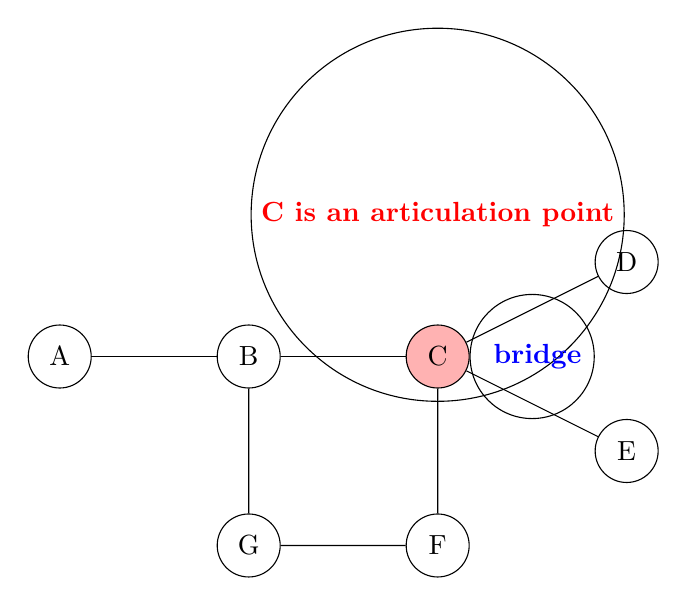
\begin{tikzpicture}[scale=1.2, every node/.style={circle, draw, minimum size=8mm}]
    % Nodes
    \node (A) at (0,0) {A};
    \node (B) at (2,0) {B};
    \node[fill=red!30] (C) at (4,0) {C}; % articulation point
    \node (D) at (6,1) {D};
    \node (E) at (6,-1) {E};
    \node (F) at (4,-2) {F};
    \node (G) at (2,-2) {G};

    % Edges
    \draw (A) -- (B);
    \draw (B) -- (C);
    \draw (C) -- (D);
    \draw (C) -- (E);
    \draw (C) -- (F);
    \draw (F) -- (G);
    \draw (G) -- (B);

    % Label
    \node at (4,1.5) {\textcolor{red}{\textbf{C is an articulation point}}};
    \node at (5,0) {\textcolor{blue}{\textbf{ bridge}}};
\end{tikzpicture}
\end{center}
\begin{minted}[
bgcolor=bgcolor1,
frame=lines,
framesep=5mm,
rulecolor=\color{black},
linenos,
numbersep=5pt,
fontsize=\normalsize
]{python}
from typing import List

def find_articulation_points(graph: dict, n: int) -> List[int]:
    """
    Finds articulation points in an undirected graph using DFS.
     Time Complexity: O(V+E)    Space Complexity: O(V)
    """
    
    ids = [-1] * n      # Discovery times of nodes
    low = [-1] * n      # Lowest ids reachable from a node
    visited = [False] * n
    is_articulation = [False] * n
    id_counter = 0      # Global id counter for assigning discovery times

    def dfs(node, parent, root):
        nonlocal id_counter
        visited[node] = True
        # Set the discovery time and low-link value
        ids[node] = low[node] = id_counter
        id_counter += 1
        children = 0  # Count of children in DFS tree

        for neighbor in graph.get(node, []):
            if neighbor == parent:
               continue   # Skip the edge back to the parent
            if not visited[neighbor]:
                children += 1
                dfs(neighbor, node, root)
                # Update low-link value based on child
                low[node] = min(low[node], low[neighbor])
                # If condition is met, node is an articulation point (not root)
                if ids[node] <= low[neighbor] and node != root:
                    is_articulation[node] = True

                # Special rule for root: it's an articulation point if it has >1 child
                if node == root and children > 1:
                    is_articulation[node] = True
            else:
                # Update low-link value due to back edge
                low[node] = min(low[node], ids[neighbor])

    for i in range(n):
        if not visited[i]:
            dfs(i, -1, i)
    return [i for i in range(n) if is_articulation[i]]
\end{minted} 

\noindent\textbf{Problem: Bridges in Graph (Tarjan's Algorithm)}
\begin{minted}[
bgcolor=bgcolor,
frame=lines,
framesep=5mm,
rulecolor=\color{black},
linenos,
numbersep=5pt,
fontsize=\normalsize
]{python}
def find_bridges(graph: dict, n: int) -> List[List[int]]:
    """
    Finds all bridges in undirected graph using DFS.
    Time Complexity: O(V+E)    Space Complexity: O(V)
    """
    ids = [-1] * n
    low = [-1] * n
    visited = [False] * n
    bridges = []
    id_counter = 0
    def dfs(node: int, parent: int):
        nonlocal id_counter
        visited[node] = True
        # Assign discovery time and low-link value
        ids[node] = low[node] = id_counter
        id_counter += 1

        # Explore neighbors
        for neighbor in graph.get(node, []):
            if neighbor == parent:
                # Don't revisit the edge we came from
                continue
            if not visited[neighbor]:
                # Recurse on unvisited neighbor
                dfs(neighbor, node)
                # Update low-link value
                low[node] = min(low[node], low[neighbor])

                # Bridge condition: no back-edge from neighbor or its subtree
                if ids[node] < low[neighbor]:
                    bridges.append([node, neighbor])
            else:
                # Update low-link value for back-edge
                low[node] = min(low[node], ids[neighbor])
    
    for i in range(n):
        if not visited[i]:
            dfs(i, -1)
    return bridges
\end{minted}

\noindent\textbf{Problem: Disjoint Set Union (DSU) with Path Compression}
\begin{minted}[
bgcolor=bgcolor10,
frame=lines,
framesep=5mm,
rulecolor=\color{black},
linenos,
numbersep=5pt,
fontsize=\normalsize
]{python}
class DSU:
    def __init__(self, n: int):
        self.parent = list(range(n))
        self.rank = [0] * n
        self.size = [1] * n  # Each node is its own set of size 1
    def find(self, x: int) -> int:
        """Finds root with path compression"""
        if self.parent[x] != x:
            self.parent[x] = self.find(self.parent[x])
        return self.parent[x]
    
    def union(self, x: int, y: int) -> bool:
        """Unions two sets, returns True if successful"""
        root_x = self.find(x)
        root_y = self.find(y)
        if root_x == root_y:
            return False  # Already connected
            
        # Union by rank
        if self.rank[root_x] < self.rank[root_y]:
            self.parent[root_x] = root_y
        elif self.rank[root_x] > self.rank[root_y]:
            self.parent[root_y] = root_x
        else:
            self.parent[root_y] = root_x
            self.rank[root_x] += 1
        return True
        
        def unionbysize(self, x, y):
        rootX = self.find(x)
        rootY = self.find(y)
        if rootX == rootY:
            return False  # Already in the same set
        # Union by size: attach smaller set under larger set
        if self.size[rootX] < self.size[rootY]:
            self.parent[rootX] = rootY
            self.size[rootY] += self.size[rootX]
        else:
            self.parent[rootY] = rootX
            self.size[rootX] += self.size[rootY]
        return True
\end{minted}

\noindent\textbf{Problem: Cycle Detection in Undirected Graph (DSU)}
\begin{minted}[
bgcolor=bgcolor5,
frame=lines,
framesep=5mm,
rulecolor=\color{black},
linenos,
numbersep=5pt,
fontsize=\normalsize
]{python}
def has_cycle_dsu(edges: List[tuple], n: int) -> bool:
    """
    Detects cycle in undirected graph using DSU.
    Time Complexity: O(E * Alpha(V)) Approx. O(E)    Space Complexity: O(V)
    """
    dsu = DSU(n)
    for u, v in edges:
        if not dsu.union(u, v):
            return True
    return False
\end{minted}

\noindent\textbf{Problem: Kruskal's MST Algorithm}
\begin{minted}[
bgcolor=bgcolor6,
frame=lines,
framesep=5mm,
rulecolor=\color{black},
linenos,
numbersep=5pt,
fontsize=\normalsize
]{python}
def kruskal_mst(edges: List[tuple], n: int) -> int:
    """
    Finds MST weight using Kruskal's algorithm with DSU.
    Time Complexity: O(E log E)    Space Complexity: O(V)
    """
    edges.sort(key=lambda x: x[2])  # Sort by weight
    dsu = DSU(n)
    mst_weight = 0
    
    for u, v, w in edges:
        if dsu.union(u, v):
            mst_weight += w
    return mst_weight
\end{minted}

\noindent\textbf{Problem: Word Ladder I (BFS)}
\begin{minted}[
bgcolor=bgcolor3,
frame=lines,
framesep=5mm,
rulecolor=\color{black},
linenos,
numbersep=5pt,
fontsize=\normalsize
]{python}
from collections import deque

def word_ladder(begin: str, end: str, word_list: List[str]) -> int:
    """
    Finds shortest transformation sequence length.
    Time Complexity: O(M^2 * N) where M=word length, N=word count
    Space Complexity: O(N)
    """
    word_set = set(word_list)
    if end not in word_set:
        return 0
        
    queue = deque([(begin, 1)])
    visited = set([begin])
    
    while queue:
        word, steps = queue.popleft()
        if word == end:
            return steps
            
        for i in range(len(word)):
            for c in 'abcdefghijklmnopqrstuvwxyz':
                next_word = word[:i] + c + word[i+1:]
                if next_word in word_set and next_word not in visited:
                    visited.add(next_word)
                    queue.append((next_word, steps + 1))
    return 0
\end{minted}

\noindent\textbf{Problem: 0/1 Matrix (Multi-source BFS)}
\begin{minted}[
bgcolor=bgcolor8,
frame=lines,
framesep=5mm,
rulecolor=\color{black},
linenos,
numbersep=5pt,
fontsize=\normalsize
]{python}
from collections import deque

def update_matrix(matrix: List[List[int]]) -> List[List[int]]:
    """
    Calculates distance to nearest 0 for each cell.
    Time Complexity: O(m*n)    Space Complexity: O(m*n)
    """
    m, n = len(matrix), len(matrix[0])
    dist = [[-1] * n for _ in range(m)]
    queue = deque()
    
    # Initialize queue with all 0s
    for i in range(m):
        for j in range(n):
            if matrix[i][j] == 0:
                dist[i][j] = 0
                queue.append((i, j))
    
    directions = [(1,0), (-1,0), (0,1), (0,-1)]
    while queue:
        x, y = queue.popleft()
        for dx, dy in directions:
            nx, ny = x + dx, y + dy
            if 0 <= nx < m and 0 <= ny < n and dist[nx][ny] == -1:
                dist[nx][ny] = dist[x][y] + 1
                queue.append((nx, ny))
    return dist
\end{minted}

\noindent\textbf{Problem: Surrounded Regions (DFS)}
\begin{minted}[
bgcolor=bgcolor5,
frame=lines,
framesep=5mm,
rulecolor=\color{black},
linenos,
numbersep=5pt,
fontsize=\normalsize
]{python}
def solve(board: List[List[str]]) -> None:
    """
    Flips surrounded 'O' to 'X' (in-place).
    Time Complexity: O(m*n)    Space Complexity: O(m*n)
    """
    if not board: return
    m, n = len(board), len(board[0])
    
    def dfs(i, j):
        if 0 <= i < m and 0 <= j < n and board[i][j] == 'O':
            board[i][j] = 'T'  # Temporary mark
            for dx, dy in [(1,0), (-1,0), (0,1), (0,-1)]:
                dfs(i+dx, j+dy)
    
    # Mark border-connected 'O's
    for i in range(m):
        dfs(i, 0)
        dfs(i, n-1)
    for j in range(n):
        dfs(0, j)
        dfs(m-1, j)
    
    # Flip inner 'O' to 'X' and restore border 'O's
    for i in range(m):
        for j in range(n):
            if board[i][j] == 'O':
                board[i][j] = 'X'
            elif board[i][j] == 'T':
                board[i][j] = 'O'
\end{minted}

\noindent\textbf{Problem: Is Graph Bipartite?}
\begin{minted}[
bgcolor=bgcolor2,
frame=lines,
framesep=5mm,
rulecolor=\color{black},
linenos,
numbersep=5pt,
fontsize=\normalsize
]{python}
def is_bipartite(graph: List[List[int]]) -> bool:
    """
    Checks if graph is bipartite using BFS coloring.
    Time Complexity: O(V+E)    Space Complexity: O(V)
    """
    n = len(graph)
    colors = [-1] * n  # -1: uncolored, 0/1: colors
    
    for i in range(n):
        if colors[i] == -1:
            queue = deque([i])
            colors[i] = 0
            while queue:
                node = queue.popleft()
                for neighbor in graph[node]:
                    if colors[neighbor] == -1:
                        colors[neighbor] = 1 - colors[node]
                        queue.append(neighbor)
                    elif colors[neighbor] == colors[node]:
                        return False
    return True
\end{minted}

\noindent\textbf{Problem: Find Eventual Safe States}
\begin{minted}[
bgcolor=bgcolor10,
frame=lines,
framesep=5mm,
rulecolor=\color{black},
linenos,
numbersep=5pt,
fontsize=\normalsize
]{python}
def eventual_safe_nodes(graph: List[List[int]]) -> List[int]:
    """
    Finds nodes that can reach terminal nodes (no cycles).
    Time Complexity: O(V+E)    Space Complexity: O(V)
    """
    n = len(graph)
    state = [0] * n  # 0: unvisited, 1: visiting, 2: safe
    
    def is_safe(node):
        if state[node] > 0:
            return state[node] == 2
        state[node] = 1  # mark as visiting
        for neighbor in graph[node]:
            if not is_safe(neighbor):  # if any neighbor leads to a cycle
                return False
        state[node] = 2  # mark as safe after exploring all neighbors
        return True
    return [i for i in range(n) if is_safe(i)]
    ###################################KAHN'S#########################################
def eventual_safe_nodes(graph: List[List[int]]) -> List[int]:
    """
    Finds eventual safe nodes using Kahn’s Algorithm (BFS + Topological Sort).
    Time Complexity: O(V + E)    Space Complexity: O(V + E)
    """
    n = len(graph)
    # Step 1: Reverse the graph
    reverse_graph = defaultdict(list)
    indegree = [0] * n
    for u in range(n):
        for v in graph[u]:
            reverse_graph[v].append(u)
            indegree[u] += 1  # original node u had an outgoing edge

    # Step 2: Start with terminal nodes (nodes with no outgoing edges originally)
    queue = deque([i for i in range(n) if indegree[i] == 0])
    safe = [False] * n  # Mark nodes proven to be safe
    while queue:
        node = queue.popleft()
        safe[node] = True
        for neighbor in reverse_graph[node]:  # Go in reversed direction
            indegree[neighbor] -= 1
            if indegree[neighbor] == 0:
                queue.append(neighbor)

    # Return sorted list of safe nodes
    return sorted([i for i, val in enumerate(safe) if val])

\end{minted}

\noindent\textbf{Problem: Alien Dictionary (Topo Sort)}
\begin{minted}[
bgcolor=bgcolor4,
frame=lines,
framesep=5mm,
rulecolor=\color{black},
linenos,
numbersep=5pt,
fontsize=\normalsize
]{python}
from collections import defaultdict, deque

def alien_order(words: List[str]) -> str:
    """
    Determines alien language order from sorted dictionary.
    Time Complexity: O(C) where C = total characters
    Space Complexity: O(1) fixed 26 letters
    """
    graph = defaultdict(set)
    indegree = defaultdict(int)
    all_chars = set(''.join(words))
    
    # Build graph and indegree
    for i in range(1, len(words)):
        a, b = words[i-1], words[i]
        min_len = min(len(a), len(b))
        for j in range(min_len):
            if a[j] != b[j]:
                if b[j] not in graph[a[j]]:
                    graph[a[j]].add(b[j])
                    indegree[b[j]] += 1
                break
        else:
            if len(a) > len(b):
                return ""  # Invalid
    
    # Kahn's algorithm
    queue = deque([c for c in all_chars if indegree.get(c, 0) == 0])
    order = []
    
    while queue:
        c = queue.popleft()
        order.append(c)
        for neighbor in graph[c]:
            indegree[neighbor] -= 1
            if indegree[neighbor] == 0:
                queue.append(neighbor)
    
    return ''.join(order) if len(order) == len(all_chars) else ""
\end{minted}

\noindent\textbf{Problem: Minimum Effort Path (BFS + Binary Search) And (Dijkstra)}
\begin{minted}[
bgcolor=bgcolor5,
frame=lines,
framesep=5mm,
rulecolor=\color{black},
linenos,
numbersep=5pt,
fontsize=\normalsize
]{python}
def minimum_effort_path(heights: List[List[int]]) -> int:
    """
    Finds min effort path (max abs diff) from top-left to bottom-right.
    Time Complexity: O(m*n*log(max_height))    Space Complexity: O(m*n)
    """
    m, n = len(heights), len(heights[0])
    low, high = 0, max(max(row) for row in heights)
    
    def can_reach(effort):
        visited = [[False] * n for _ in range(m)]
        queue = deque([(0,0)])
        visited[0][0] = True
        directions = [(1,0), (-1,0), (0,1), (0,-1)]
        
        while queue:
            x, y = queue.popleft()
            if x == m-1 and y == n-1:
                return True
            for dx, dy in directions:
                nx, ny = x+dx, y+dy
                if 0 <= nx < m and 0 <= ny < n and not visited[nx][ny]:
                    diff = abs(heights[x][y] - heights[nx][ny])
                    if diff <= effort:
                        visited[nx][ny] = True
                        queue.append((nx, ny))
        return False
    
    while low < high:
        mid = (low + high) // 2
        if can_reach(mid):
            high = mid
        else:
            low = mid + 1
    return low
                     #########################################

def minimum_effort_path(heights: List[List[int]]) -> int:
    """
    Dijkstra-based solution for minimum effort path.
    Each move has an 'effort' = abs height difference.
    We seek the path with minimum *maximum* effort along the path.
    """
    m, n = len(heights), len(heights[0])
    # Min-heap priority queue: (effort_so_far, x, y)
    heap = [(0, 0, 0)]    
    # Tracks minimum effort to reach each cell
    effort_to = [[float('inf')] * n for _ in range(m)]
    effort_to[0][0] = 0
    directions = [(-1, 0), (1, 0), (0, -1), (0, 1)]
    while heap:
        effort, x, y = heapq.heappop(heap)

        # If we reached bottom-right cell, return the effort
        if x == m - 1 and y == n - 1:
            return effort
        
        for dx, dy in directions:
            nx, ny = x + dx, y + dy
            if 0 <= nx < m and 0 <= ny < n:
                # Calculate effort to move to neighbor
                current_diff = abs(heights[nx][ny] - heights[x][y])
                max_effort = max(effort, current_diff)
                
                # If this path is better, update and add to heap
                if effort_to[nx][ny] > max_effort:
                    effort_to[nx][ny] = max_effort
                    heapq.heappush(heap, (max_effort, nx, ny))
    return -1  

\end{minted}

\noindent\textbf{Problem: Make a Large Island}
\begin{minted}[
bgcolor=bgcolor6,
frame=lines,
framesep=5mm,
rulecolor=\color{black},
linenos,
numbersep=5pt,
fontsize=\normalsize
]{python}
def largest_island(grid: List[List[int]]) -> int:
    """
    Finds largest island after changing at most one 0 to 1.
    Time Complexity: O(m*n)    Space Complexity: O(m*n)
    """
    m, n = len(grid), len(grid[0])
    island_id = 2  # Start from 2 (0/1 are used)
    area = defaultdict(int)
    directions = [(1,0), (-1,0), (0,1), (0,-1)]
    
    # DFS to mark islands and record areas
    def dfs(i, j, id):
        if 0 <= i < m and 0 <= j < n and grid[i][j] == 1:
            grid[i][j] = id
            count = 1
            for dx, dy in directions:
                count += dfs(i+dx, j+dy, id)
            return count
        return 0
    
    # Mark all islands and store their sizes
    for i in range(m):
        for j in range(n):
            if grid[i][j] == 1:
                area[island_id] = dfs(i, j, island_id)
                island_id += 1
    
    max_area = max(area.values()) if area else 0
    for i in range(m):
        for j in range(n):
            if grid[i][j] == 0:
                seen_ids = set()
                for dx, dy in directions:
                    ni, nj = i+dx, j+dy
                    if 0 <= ni < m and 0 <= nj < n and grid[ni][nj] > 1:
                        seen_ids.add(grid[ni][nj])
                total = 1 + sum(area[id] for id in seen_ids)
                max_area = max(max_area, total)
    return max_area
\end{minted}

\noindent\textbf{Problem: Cheapest Flights Within K Stops}
\begin{minted}[
bgcolor=bgcolor3,
frame=lines,
framesep=5mm,
rulecolor=\color{black},
linenos,
numbersep=5pt,
fontsize=\normalsize
]{python}
def find_cheapest_price(n: int, flights: List[List[int]], src: int, dst: int, k: int) -> int:
    """
    Finds cheapest flight with at most k stops using Bellman-Ford.
    Time Complexity: O(K * E)    Space Complexity: O(n)
    """
    prices = [float('inf')] * n
    prices[src] = 0
    
    # Relax edges k+1 times
    for _ in range(k+1):
        temp = prices[:]  # Copy current state
        for u, v, w in flights:
            if prices[u] != float('inf'):
                temp[v] = min(temp[v], prices[u] + w)
        prices = temp
    
    return prices[dst] if prices[dst] != float('inf') else -1
                     #########################################
def find_cheapest_price(n: int, flights: List[List[int]],src: int,dst: int,K: int) -> int:
    """
    Modified Dijkstra to find the cheapest flight with at most K stops.
    Uses (cost, node, stops) in the min-heap.
    """
    # Build adjacency list: u -> [(v, price)]
    graph = defaultdict(list)
    for u, v, price in flights:
        graph[u].append((v, price))
    
    # Min-heap: (total_cost, current_city, stops_so_far)
    heap = [(0, src, 0)]
    
    # Use a dict to track best cost at (city, stops)
    visited = dict()

    while heap:
        cost, city, stops = heapq.heappop(heap)
        # If destination reached within allowed stops, return the cost
        if city == dst:
            return cost
        # If already visited with fewer stops, skip (to avoid cycles and inefficiency)
        if (city, stops) in visited and visited[(city, stops)] <= cost:
            continue
        visited[(city, stops)] = cost

        # Only proceed if stops are within limit
        if stops <= K:
            for neighbor, price in graph[city]:
                new_cost = cost + price
                heapq.heappush(heap, (new_cost, neighbor, stops + 1))
    return -1
\end{minted}

\noindent\textbf{Problem: Number of Ways to Arrive at Destination}
\begin{minted}[
bgcolor=bgcolor,
frame=lines,
framesep=5mm,
rulecolor=\color{black},
linenos,
numbersep=5pt,
fontsize=\normalsize
]{python}
def count_paths(n: int, roads: List[List[int]]) -> int:
    """
    Counts number of shortest paths from 0 to n-1.
    Time Complexity: O(E log V)    Space Complexity: O(V)
    """
    MOD = 10**9 + 7
    graph = defaultdict(list)
    for u, v, time in roads:
        graph[u].append((v, time))
        graph[v].append((u, time))
    
    dist = [float('inf')] * n
    ways = [0] * n
    dist[0] = 0
    ways[0] = 1
    heap = [(0, 0)]
    
    while heap:
        d, node = heapq.heappop(heap)
        if d != dist[node]:
            continue
        for neighbor, time in graph[node]:
            new_dist = d + time
            if new_dist < dist[neighbor]:
                dist[neighbor] = new_dist
                ways[neighbor] = ways[node]
                heapq.heappush(heap, (new_dist, neighbor))
            elif new_dist == dist[neighbor]:
                ways[neighbor] = (ways[neighbor] + ways[node]) % MOD
    return ways[n-1] % MOD
\end{minted}
% \end{document}

\newgeometry{margin=0.2in}
\clearpage
\section{Trie,Segment and Binary Indexed Tree-Based DSA Problems Summary Table}
\begin{longtable}{|>{\raggedright\arraybackslash}p{3.2cm}|>{\columncolor{c2}\centering\arraybackslash}p{2.5cm}|>{\columncolor{c3}\raggedright\arraybackslash}p{4.3cm}|>{\columncolor{c4}\raggedright\arraybackslash}p{3.5cm}|>{\columncolor{c5}\color{white}\raggedright\arraybackslash}p{3.5cm}|}
\hline
\rowcolor{rclr}
\textbf{Problem Name} & \textbf{Time Complexity} & \textbf{Idea to Solve} & \textbf{Optimization Tip} & \textbf{Edge Cases} \\
\hline
\endfirsthead
\hline
\textbf{Problem Name} & \textbf{Time Complexity} & \textbf{Idea to Solve} & \textbf{Optimization Tip} & \textbf{Edge Cases} \\
\hline
\endhead
Insert a Word in Trie & $O(L)$ & Traverse from root, create nodes for each char if absent & Use array/map for children & Empty word, existing prefix \\
\hline
Search a Word in Trie & $O(L)$ & Traverse char by char, return false if node missing, else check end flag & Store end-of-word boolean & Word exists as prefix but not complete \\
\hline
Delete a Word in Trie & $O(L)$ & Recursively delete only if no children and not end of another word & Track if node can be deleted during backtracking & Deleting prefix of other word \\
\hline
Autocomplete Suggestions & $O(L + k)$ & Traverse to prefix node, do DFS/BFS to collect $k$ words & Add lexicographical ordering for sorted output & Prefix not found or no suggestions \\
\hline
Count Distinct Rows in Binary Matrix & $O(n \cdot m)$ & Insert each row into a Trie (0/1 as path), count unique terminations & Use Trie instead of set for space efficiency & Duplicate rows \\
\hline
Max XOR of 2 Elements & $O(n \cdot \log M)$ & Insert bits into Trie; for each, find best XOR & Use 31-bit mask for int range & All numbers same \\
\hline
Max XOR with Given Query & $O(n \cdot \log M)$ & For each query, insert eligible elements to Trie & Sort queries + elements & No valid element for query \\
\hline
Count Different Substrings & $O(n^2)$ & Use Suffix Trie/Automaton or HashSet of substrings & Use rolling hash for faster check & All characters same \\
\hline
\end{longtable}
\clearpage
\newgeometry{margin=1in}
% \documentclass[a4paper,10pt]{article}
% \usepackage[utf8]{inputenc}
% \usepackage{geometry}
% \usepackage[table]{xcolor}
% \usepackage{colortbl}
% \usepackage{color,soul}
% \geometry{margin=0.8in}
% \usepackage{xcolor}
% \usepackage{tikz}
% \usepackage{minted}
% \definecolor{bgcolor}{rgb}{0.8, 0.9, 0.5} % 
% \definecolor{bgcolor1}{rgb}{0.95, 0.95, 0.95} % Light Gray
% \definecolor{bgcolor2}{rgb}{0.85, 0.92, 1.0}  % Soft Blue
% \definecolor{bgcolor3}{rgb}{0.9, 0.85, 1.0}   % Light Purple
% \definecolor{bgcolor4}{rgb}{0.95, 0.88, 0.76} % Warm Beige
% \definecolor{bgcolor5}{rgb}{0.8, 0.95, 0.8}   % Gentle Green
% \definecolor{bgcolor6}{rgb}{1.0, 0.87, 0.87}  % Pastel Red
% \definecolor{bgcolor7}{rgb}{0.86, 0.93, 0.83} % Mint Green
% \definecolor{bgcolor8}{rgb}{0.98, 0.85, 0.94} % Soft Pink
% \definecolor{bgcolor9}{rgb}{0.87, 0.94, 0.98} % Sky Blue
% \definecolor{bgcolor10}{rgb}{0.96, 0.96, 0.82} % Pale Yellow
% 
% \begin{document}
\section*{Tries and Binary Index Tree Problem Solutions}


\noindent\textbf{Problem: Tries Operation}
\begin{minted}[
bgcolor=bgcolor3,
frame=lines,
framesep=5mm,
rulecolor=\color{black},
linenos,
numbersep=5pt,
fontsize=\normalsize
]{python}  
class TrieNode:
    def __init__(self):
        self.children = {}
        self.is_end_of_word = False

class Trie:
    def __init__(self):
        self.root = TrieNode()

     def insert(self, word):
        node = self.root
        for char in word:
            if char not in node.children:
                node.children[char] = TrieNode()
            node = node.children[char]
        node.is_end_of_word = True

    def search(self, word):
        node = self.root
        for char in word:
            if char not in node.children:
                return False
            node = node.children[char]
        return node.is_end_of_word

    def delete(self, word):
        def _delete(node, word, depth):
            if depth == len(word):
                if not node.is_end_of_word:
                    return False
                node.is_end_of_word = False
                return len(node.children) == 0
            char = word[depth]
            if char not in node.children:
                return False
            should_delete = _delete(node.children[char], word, depth + 1)
            if should_delete:
                del node.children[char]
                return not node.is_end_of_word and len(node.children) == 0
            return False

        _delete(self.root, word, 0)
\end{minted}
\noindent\textbf{Auto Complete Suggestions}
\begin{minted}[
bgcolor=bgcolor1,
frame=lines,
framesep=5mm,
rulecolor=\color{black},
linenos,
numbersep=5pt,
fontsize=\normalsize
]{python}
# Method to search the Trie for a prefix and return the node where prefix ends
    def _search_prefix_node(self, prefix):
        node = self.root
        for char in prefix:
            if char in node.children:
                node = node.children[char]
            else:
                # If prefix is not in trie, return None
                return None
        return node

    # Recursive helper to collect all words starting from a given node
    def _collect_all_words(self, node, prefix, results):
        if node.is_end_of_word:
            results.append(prefix)
        for char, next_node in node.children.items():
            # Continue the search with extended prefix
            self._collect_all_words(next_node, prefix + char, results)

    # Public method to get autocomplete suggestions for a prefix
    def autocomplete(self, prefix):
        results = []
        # Find the node where the prefix ends
        prefix_node = self._search_prefix_node(prefix)
        if not prefix_node:
            return []  # No suggestions if prefix doesn't exist
        # Collect all words from that node
        self._collect_all_words(prefix_node, prefix, results)
        return results
\end{minted}
\noindent\textbf{Problem: Count Distinct Rows in Binary Matrix}
\begin{minted}[
bgcolor=bgcolor5,
frame=lines,
framesep=5mm,
rulecolor=\color{black},
linenos,
numbersep=5pt,
fontsize=\normalsize
]{python}
class Trie:
    def __init__(self):
        self.root = TrieNode()

    # Insert a row into the Trie
    # Returns True if it's a new row, False if duplicate
    def insert(self, row):
        node = self.root
        is_new = False  # Flag to track if row is unique

        for bit in row:
            # If the child node for current bit doesn't exist, create it
            if node.children[bit] is None:
                node.children[bit] = TrieNode()
                is_new = True  # Since a new node was created, it's a new path
            node = node.children[bit]

        # If end-of-row flag is not yet set, it's a new row
        if not node.is_end_of_row:
            node.is_end_of_row = True
            is_new = True

        return is_new

# Function to count distinct rows using Trie
def count_distinct_rows(matrix):
    trie = Trie()
    count = 0

    for row in matrix:
        if trie.insert(row):
            count += 1  # Row is distinct

    return count
\end{minted}

\noindent\textbf{Problem: Maximum Xor of 2 Elements in Array}
\begin{minted}[
bgcolor=bgcolor6,
frame=lines,
framesep=5mm,
rulecolor=\color{black},
linenos,
numbersep=5pt,
fontsize=\normalsize
]{python}
# Define the number of bits (32 for standard int)
INT_SIZE = 32

# Trie Node for storing binary digits
class TrieNode:
    def __init__(self):
        self.children = [None, None]  # 0 and 1

# Trie structure for inserting and querying
class Trie:
    def __init__(self):
        self.root = TrieNode()

    # Insert number into the Trie
    def insert(self, num):
        node = self.root
        for i in reversed(range(INT_SIZE)):  # From MSB to LSB
            bit = (num >> i) & 1
            if node.children[bit] is None:
                node.children[bit] = TrieNode()
            node = node.children[bit]

    # Find max XOR of num with elements already in Trie
    def max_xor(self, num):
        node = self.root
        max_xor = 0
        for i in reversed(range(INT_SIZE)):
            bit = (num >> i) & 1
            # Prefer opposite bit to maximize XOR
            toggled_bit = 1 - bit
            if node.children[toggled_bit]:
                max_xor |= (1 << i)  # Add this bit to result
                node = node.children[toggled_bit]
            else:
                node = node.children[bit]
        return max_xor

# Main function to find max XOR of any two numbers
def find_max_xor(arr):
    trie = Trie()
    max_result = 0

    # Insert the first number before comparisons
    trie.insert(arr[0])

    for num in arr[1:]:
        # Check current max XOR
        current_xor = trie.max_xor(num)
        max_result = max(max_result, current_xor)
        # Insert current number into Trie
        trie.insert(num)

    return max_result
\end{minted}

\noindent\textbf{Problem: Distinct Substring in a String}\\
Every substring of a string is a prefix of some suffix — but not every substring is a prefix of the original string.
\begin{minted}[
bgcolor=bgcolor10,
frame=lines,
framesep=5mm,
rulecolor=\color{black},
linenos,
numbersep=5pt,
fontsize=\normalsize
]{python}
# Trie Node class
class TrieNode:
    def __init__(self):
        self.children = {}  # Dictionary for character links

# Trie class to insert and count distinct substrings
class Trie:
    def __init__(self):
        self.root = TrieNode()
        self.count = 0  # To count new nodes (distinct substrings)

    # Insert a suffix into the Trie and count new substrings
    def insert_suffix(self, suffix):
        node = self.root
        for char in suffix:
            # If char is not present, it's a new substring
            if char not in node.children:
                node.children[char] = TrieNode()
                self.count += 1  # New substring added
            node = node.children[char]

# Function to count all distinct substrings of a string
def count_distinct_substrings(s):
    trie = Trie()

    # Insert all suffixes into the Trie
    for i in range(len(s)):
        suffix = s[i:]
        trie.insert_suffix(suffix)

    # Total distinct substrings = total nodes created in Trie
    return trie.count
\end{minted}
\noindent\textbf{Problem: Binary Index Tree(tushar)}
\begin{minted}[
bgcolor=bgcolor5,
frame=lines,
framesep=5mm,
rulecolor=\color{black},
linenos,
numbersep=5pt,
fontsize=\normalsize
]{python}

\end{minted}
% \end{document}

\newgeometry{margin=0.2in}
\clearpage
\end{document}
